\documentclass[a4paper,10pt]{article}
\usepackage[utf8]{inputenc}
\usepackage{graphicx}
\usepackage[thinlines]{easytable}
\usepackage{enumitem}
\usepackage{amsmath}
\usepackage{amsfonts}
\usepackage{graphicx}
\usepackage{bbm}
\usepackage{textcomp}
\usepackage{relsize}
\usepackage{listings}
\usepackage[usenames,dvipsnames]{color}
\usepackage{mathtools}
\usepackage{multicol}
\setcounter{MaxMatrixCols}{20}
\allowdisplaybreaks
%%%%%%%%%%%%%%%%%%%%%%%%%%%%%%%%%%%%%%%%%%%%%%%%%%%%%%%%%%%%%%%%%%%%%%%%%%%%%%%%%%%%%%%%%%%
% MATLAB code listing
%
% This is the color used for MATLAB comments below
\definecolor{MyDarkGreen}{rgb}{0.0,0.4,0.0}
 
% For faster processing, load Matlab syntax for listings
\lstloadlanguages{Matlab}%
\lstset{language=Matlab, % Use MATLAB
frame=single, % Single frame around code
basicstyle=\tiny\ttfamily, % Use small true type font
keywordstyle=[1]\color{Blue}\bfseries, % MATLAB functions bold and blue
keywordstyle=[2]\color{Purple}, % MATLAB function arguments purple
keywordstyle=[3]\color{Blue}\underbar, % User functions underlined and blue
identifierstyle=, % Nothing special about identifiers
% Comments small dark green courier
commentstyle=\usefont{T1}{pcr}{m}{sl}\color{MyDarkGreen}\tiny,
stringstyle=\color{Purple}, % Strings are purple
showstringspaces=false, % Don't put marks in string spaces
tabsize=5, % 5 spaces per tab
%
%%% Put standard MATLAB functions not included in the default
%%% language here
morekeywords={xlim,ylim,var,alpha,factorial,poissrnd,normpdf,normcdf},
%
%%% Put MATLAB function parameters here
morekeywords=[2]{on, off, interp},
%
%%% Put user defined functions here
morekeywords=[3]{FindESS, homework_example},
%
morecomment=[l][\color{Blue}]{...}, % Line continuation (...) like blue comment
numbers=left, % Line numbers on left
firstnumber=1, % Line numbers start with line 1
numberstyle=\tiny\color{Blue}, % Line numbers are blue
stepnumber=5 % Line numbers go in steps of 5
}
%%%%%%%%%%%%%%%%%%%%%%%%%%%%%%%%%%%%%%%%%%%%%%%%%%%%%%%%%%%%%%%5


\newcommand\scalemath[2]{\scalebox{#1}{\mbox{\ensuremath{\displaystyle #2}}}}
% \scalemath{1.0}

%opening
\title{Equations Of Motion of Krang}
\author{Munzir Zafar}

\begin{document}

\maketitle

In this report we attempt to find the dynamic model of Golem Krang. It is a serial robot with a tree-structure (due to two arms branching out) that is balanced on two wheels as an inverted pendulum. So it is a humanoid insofar as it is bimanual and dynamically stable (i.e. an inverted pendulum). But it has two wheels instead of two legs. Figure \ref{fig:frames} shows the frames of references we will be using to determine the transforms and the coordinates on the robot. Also $\dot{x}$ is the heading speed of the robot and $\dot\psi$ is the spin speed of the robot. We denote these frames using symbol $R_i$ where $i \in \mathbb{F} = \lbrace 0$, $1$, $2$, $3$, $4l$, $5l$, $6l$, $7l$, $8l$, $9l$, $10l$, $4r$, $5r$, $6r$, $7r$, $8r$, $9r$, $10r \rbrace$. $R_0$ is the world frame fixed in the middle of the two wheels. $R_1, R_2, R_3$ are fixed on the base, spine and torso with their rotations represented by $q_{imu}$, $q_w$ and $q_{torso}$ respectively. Frames $R_{4l}, ... R_{10l}$ are frames fixed on the links 
left 7-DOF arm with their motion represented by $q_{1l}, ... q_{7l}$. Similarly, frames $R_{4r}, ... R_{10r}$ are frames fixed on the links right 7-DOF arm with their motion represented by $q_{1r}, ... q_{7r}$.  All equations in the 
following text that do not show $r$ or $l$ in the subscript where they are supposed to, will mean that the respective equations are valid for both subscripts.

\begin{figure}
 \centering
 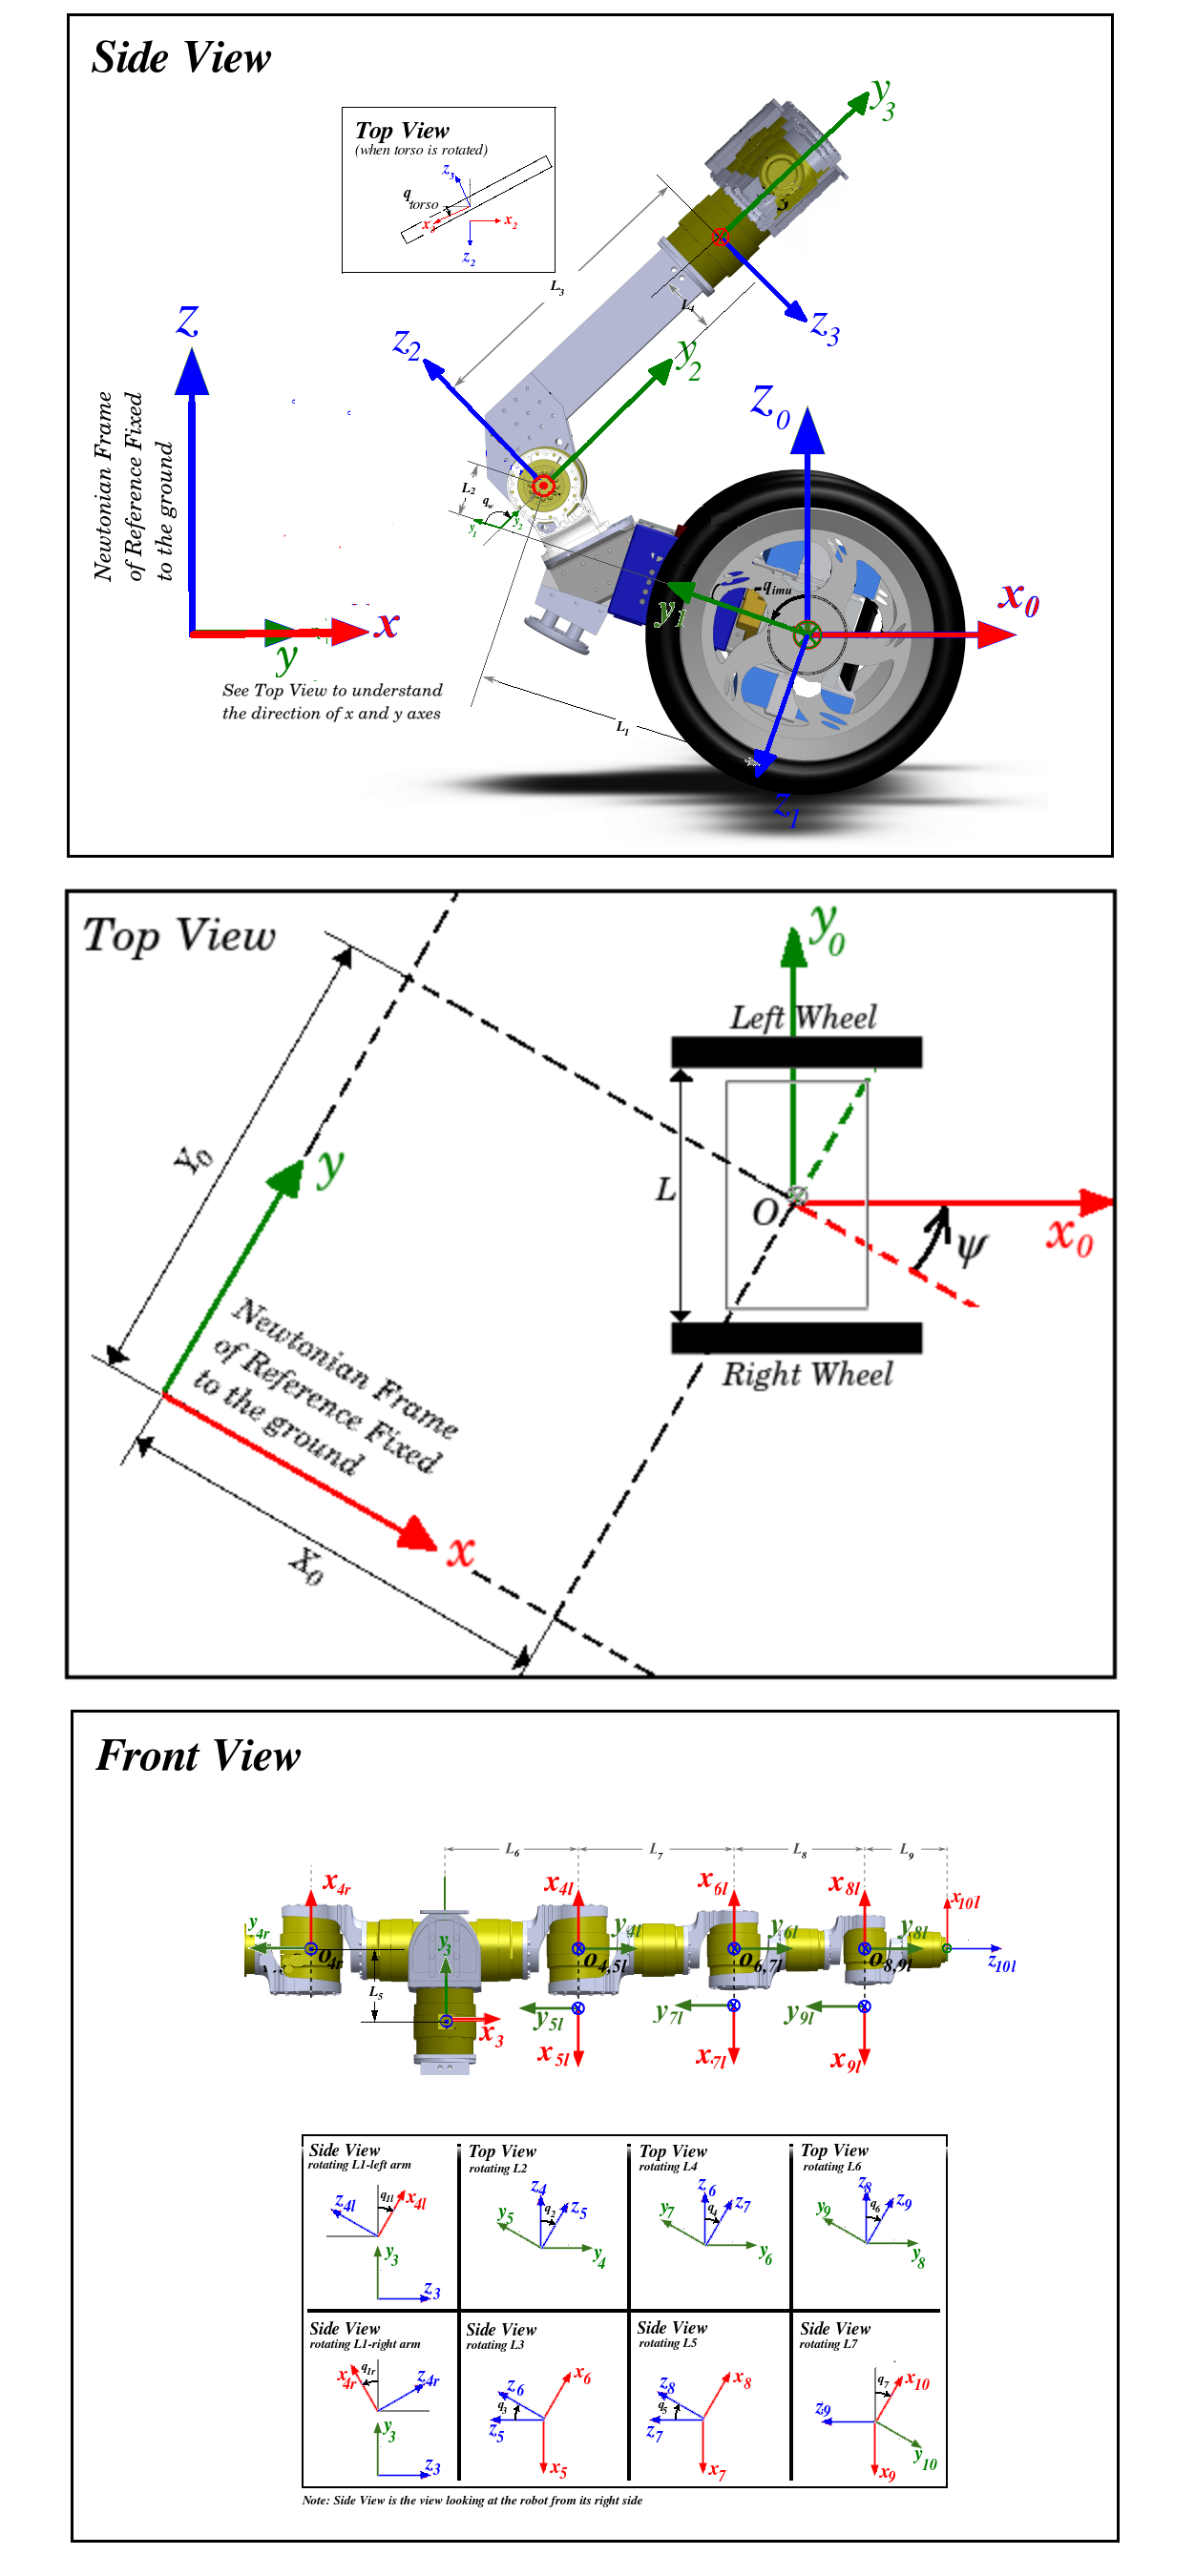
\includegraphics[width=0.8\textwidth]{Figures/frames.png}
 \caption{Frames of references on the robot}
 \label{fig:frames}
\end{figure}

\section{Generalized Coordinates}

We select twenty-one generalized co-ordinates: $\{q\} = \{$ $X_0$, $Y_0$, $\theta_L$, $\theta_R$, $q_{imu}$, $q_{w}$, $q_{torso}$, $q_{1l}$, $...$, $q_{7l}$, $q_{1r}$, $...$, $q_{7r} \}$. Where:
\begin{itemize}[label={}]
 \item[$X_0, Y_0$] are the position coordintes of $O$ wrt a Newtonian reference frame $xyz$ fixed on ground
 \item[$\theta_L, \theta_R$] are the rotation angles of the left and right wheels respectively
\end{itemize}

Given this Newtonian frame of reference we can define $\psi$ as the heading direction ($x_0$) measured as
an angle from the $x$-axis of the Newtonian frame.

\section{Constraint Equations}
Let $\bar{i}_0$, $\bar{j}_0$ and $\bar{k}_0$ be the unit vectors in frame $x_0y_0z_0$ and $\bar{I}$, $\bar{J}$ and 
$\bar{K}$ be the unit vectors in frame $xyz$.

Under the assumption of no slipping/skidding, we have two constraint equations:

\begin{align} 
 \bar{v}_L &= R\dot\theta_L\bar{i}_0 \label{constraintOne}\\
 \bar{v}_R &= R\dot\theta_R\bar{i}_0 \label{constraintTwo}
\end{align}

Since
\begin{align}
 \bar{v}_L &= \bar{v}_0 + \bar\omega_0 \times \bar{r}_{L/O} \nonumber \\
 &= \dot{X}_0 \bar{I} + \dot{Y}_0 \bar{J} + \dot{\psi} \bar{K} \times (\frac{L}{2}\bar{j}_0) \nonumber \\
 &= \dot{X}_0 (cos\psi\bar{i}_0 - sin\psi\bar{j}_0) + \dot{Y}_0 (sin\psi\bar{i}_0+cos\psi\bar{k}_0) - \frac{L}{2}\dot{\psi} \bar{i}_0 \nonumber \\
 &= (\dot{X}_0 cos\psi + \dot{Y}_0 sin\psi - \frac{L}{2}\dot{\psi}) \bar{i}_0 - (\dot{X}_0 sin\psi - \dot{Y}_0 cos\psi)\bar{j}_0 \nonumber 
\end{align}

And similarly,
\begin{align}
 \bar{v}_R  &= (\dot{X}_0 cos\psi + \dot{Y}_0 sin\psi + \frac{L}{2}\dot{\psi}) \bar{i}_0 - (\dot{X}_0 sin\psi - \dot{Y}_0 cos\psi)\bar{j}_0 \nonumber 
\end{align}

Comparing the coefficients of $\bar{i}_0$ in eqs. \ref{constraintOne}-\ref{constraintTwo} gives:
\begin{align}
 \dot{X}_0 cos\psi + \dot{Y}_0 sin\psi - \frac{L}{2}\dot{\psi} &= R\dot\theta_L \label{thetaL} \\
 \dot{X}_0 cos\psi + \dot{Y}_0 sin\psi + \frac{L}{2}\dot{\psi} &= R\dot\theta_R \label{thetaR} 
\end{align}
Subtraction and addition of the two equations gives us:
\begin{align}
 \dot{\psi} &= \frac{R}{L}(\dot\theta_R - \dot\theta_L) \label{psiThetaRelationship} \\
 \dot{X}_0 cos\psi + \dot{Y}_0 sin\psi &= \frac{R}{2}(\dot\theta_L + \dot\theta_R) \label{constraint1} 
\end{align}
Eq. \ref{psiThetaRelationship} can be integrated to give $\psi = \frac{R}{L}(\theta_R - \theta_L)$ which can be substituted in
eq. \ref{constraint1} to give our first constraint equation relating the first four generalized co-ordinates.

Comparing the coefficients of $\bar{j}_0$ in eqs. \ref{constraintOne}-\ref{constraintTwo} gives us our second constraint equation:
\begin{align}
 \dot{X}_0 sin\psi - \dot{Y}_0 cos\psi &= 0 \label{constraint2}
\end{align}

Eqs. \ref{constraint1}-\ref{constraint2} give the two constraint equations relating our generalized velocities as a 
result of the nonholonomic constrainsts. Twenty-one generalized coordinates with two constraint equations leads
to nineteen degrees of freedom.

\section{Defining Generalized Velocities}
It is easier to derive the dynamic model of the system in terms of the generalized velocities:
$\{\dot{q}\} = \{$ $\dot{x}$, $\dot{\psi}$, $\dot{q}_{imu}$, $\dot{q}_{w}$, $\dot{q}_{torso}$, $\dot{q}_{1l}$, $...$, $\dot{q}_{7l}$, $\dot{q}_{1r}$, $...$, $\dot{q}_{7r} \}$. 
These nineteen velocities can take
arbitrary values all of whom will be kinematically admissible. In other words, they represent
our nineteen degrees of freedom. Here $\dot{x}$ should be refered
to as a quasi-velocity as this velocity has meaning only as a velocity but its corresponding
position variable $x$ does not give any physical meaning. Although, the infinitesimal change of
position $\delta x = \dot{x} dt$ (sometimes refered to as virtual displacement) has physical
meaning.

The older generalized velocities can be calculated from the new ones as follows:
\begin{align}
 \dot{X}_0 &= \dot{x}cos\psi \label{relStart}\\
 \dot{Y}_0 &= \dot{x}sin\psi \\
 \dot\theta_L &= \frac{1}{R}\dot{x} - \frac{L}{2R}\dot{\psi} \\
 \dot\theta_R &= \frac{1}{R}\dot{x} + \frac{L}{2R}\dot{\psi} \label{relEnd}
\end{align}
Where the first two relationships are derived by comparing the coefficients in 
$\dot{X}_0\bar{I}+\dot{Y}_0\bar{J} = \bar{v}_0 = \dot{x}\bar{i}_0 = \dot{x}(cos\psi\bar{I}+sin\psi\bar{J})$.
And the next
two relationships are derived by substituting the the first two relationships in eqs. \ref{thetaL}-\ref{thetaR}.
When these relationships (\ref{relStart}-\ref{relEnd}) are substituted in our constraint equations \ref{constraint1}-\ref{constraint2}, both
sides of the equations vanish. Indicating that these twenty degrees of freedom are not bound by any constraint.
We will now derive nineteen dynamic equations in terms of our new generalized velocities. Those equations in
conjunction with these relationships can solve for all twenty-two generalized coordinates.

We will be using the Kane's formulation. This is done because the presence of quasi-velocity prohibits us from using Lagrange method for dynamic modeling.

\section{Introduction to Kane's Formulation}
\begin{align}
 \sum_{\substack{k}} \left[ m_k \bar{a}_{Gk} \cdot \left(\bar{v}_{Gk}\right)_j + \left( \frac{d\bar{H}_{Gk}}{dt} 
 \right) \cdot \left( \bar\omega_k \right)_j \right] = \sum_{\substack{n}}  \bar{F}_n \cdot \left( \bar{v}_n \right)_j 
 + \sum_{\substack{n}}  \bar{M}_m \cdot \left( \bar{\omega}_m \right)_j \;\; j=1 ... K \label{kanes}
\end{align}
where 
\begin{itemize}[label={}]
\item[$j$] is the unique number identifying each generalized co-ordinate in the system
\item[$k$] is the unique number identifying each rigid body in the system
\item[$n$] is the unique number identifying each external force acting on the system
\item[$m$] is the unique number identifying each external torque acting on the system
\item[$m_k$] is the mass of the $k$th body
\item[$\bar{a}_{Gk}$] is the acceleration of the center of mass of $k$th body
\item[$\bar{v}_{Gk}$] is the velocity of the center of mass of the $k$th body
\item[$\bar{H}_{Gk}$] is the angular momentum of body $k$ about its center of mass
\item[$\bar{\omega}_{k}$] is the angular velocity of the body $k$
\item[$F_n$] is the $n$th external force
\item[$M_m$] is the $m$th external moment
\item[$\bar{v}_{n}$] is the velocity of the point at which external Force $F_n$ is acting
\item[$\bar{\omega}_{m}$] is the angular velocity of the body on which torque is acting relative to the actuator applying the torque
\item[$()_j$] $=\frac{\partial ()}{\partial \dot{q}_j}$ the partial derivative of the quantity in brackets $()$ with respect to the generalized
velocity $\dot{q}_j$
\end{itemize}


\section{Kane's Left Hand Side}

The left hand side of the Kane's equation containes a sum whose range is equal to the number of bodies in the system. We have nineteen bodies: Left-wheel ($L$), right wheel ($R$) and the seventeen links in the tree structure of robot each having a frame $R_i$ fixed on it where $i \in \{ 1, 2, 3, 4l, ... 10l, 4r, ... 10r \}$. Each term in the sum consists of the acceleration ($\bar{a}_{Gk}$), velocity ($\bar{v}_{Gk}$), angular momentum ($\bar{H}_{Gk}$) of the center of mass and the body's angular velocity ($\bar{\omega}_k$). And then some partial derivatives wrt to the generalized velocities ($(\bar{\omega}_k)_j=\frac{\partial \bar{\omega}_k}{\partial \dot{q}_j}$ and $(\bar{v}_{Gk})_j=\frac{\partial \bar{v}_{Gk}}{\partial \dot{q}_j}$). We will have nineteen equations corresponding to each generalized coordinate $\{\dot{q}\} = \{$ $\dot{x}$, $\dot{\phi}$, $\dot{\psi}$, $\dot{q}_{imu}$, $\dot{q}_{w}$, $\dot{q}_{torso}$, $\dot{q}_{1l}$, $...$, $\dot{q}_{7l}$, $\dot{q}_{1r}$, $...$, $\dot{q}_{7r} \}$.

\subsection{Frame $x_0y_0z_0$} \label{frame0}

The velocities and accelerations of the frame $x_0y_0z_0$ are needed to evaluate the afore-mentioned quantities related to each body. These velocities are as follows:

\begin{align}
 \bar\omega_0 &= \dot\psi\bar{k}_0 \\
 \bar{v}_0 &= \dot{x}\bar{i}_0 \\
 \bar\alpha_0 &= \ddot\psi\bar{k}_0 \\
 \bar{a}_0 &= \ddot{x}\bar{i}_0 + \dot{x}\left( \dot\psi\bar{k}_0 \times \bar{i}_0 \right) \nonumber \\
 &= \ddot{x}\bar{i}_0 + \dot{x}\dot\psi\bar{j}_0
\end{align}

\subsection{Wheels}

\subsubsection{Left Wheel}
This evaluation takes place in the $x_Ly_Lz_L$ frame fixed to the left wheel such that it is parallel to 
frame $x_0y_0z_0$ when $\theta_L = 0$. So $\bar{i}_0 = cos\theta_L\bar{i}_L+sin\theta_L\bar{k}_L$, 
$\bar{j}_0 = \bar{j}_L$ and $\bar{k}_0 = -sin\theta_L\bar{i}_L+cos\theta_L\bar{k}_L$.
Angular velocity:
\begin{align}
 \bar{\omega}_L &= \dot\psi\bar{k}_0 + \dot\theta_L\bar{j_0} \nonumber \\
 &= \dot\psi\bar{k}_0 + \left(\frac{1}{R}\dot{x}-\frac{L}{2R}\dot\psi\right)\bar{j}_0 \nonumber \\
 &= -\dot\psi sin\theta_L\bar{i}_L + \left(\frac{1}{R}\dot{x}-\frac{L}{2R}\dot\psi\right)\bar{j}_L + \dot\psi cos\theta_L\bar{k}_L \label{kanesLHSVariableStart}
\end{align}
The terms that follow are also similarly to be expressed in frame $x_Ly_Lz_L$ but that step is skipped for brevity.
Velocity:
\begin{align}
  \bar{v}_{GL} &= \bar{v}_0 + \bar{\omega}_0 \times \bar{r}_{L/O} \nonumber \\
 &= \dot{x}\bar{i}_0 + \dot\psi\bar{k}_0 \times \frac{L}{2}\bar{j}_0 \nonumber \\
 &= \left(\dot{x}-\frac{L}{2}\dot\psi\right)\bar{i}_0  
\end{align}
Linear acceleration:
\begin{align}
 \bar{a}_{GL} &= \bar{a}_0 + \bar\alpha_0 \times \bar{r}_{L/O} + \bar\omega_0 \times \left( \omega_0 \times \bar{r}_{L/O}\right) \nonumber \\
 &= \ddot{x}\bar{i}_0 + \dot{x}\left(\dot\psi\bar{k}_0 \times \bar{i}_0\right)+ \ddot\psi\bar{k}_0 \times \frac{L}{2}\bar{j}_0 + \dot\psi\bar{k}_0 \times \left( \dot\psi\bar{k}_0 \times \frac{L}{2}\bar{j}_0\right) \nonumber \\
 &= \left(\ddot{x}-\frac{L}{2}\ddot\psi\right)\bar{i}_0 + \left(\dot{x}\dot\psi- \frac{L}{2}\dot\psi^2\right)\bar{j}_0  
\end{align}
Angular momentum and its derivative:
\begin{align}
 \bar{H}_{GL} &= I_w\bar{\omega}_L \nonumber \\
 \frac{d\bar{H}_{GL}}{dt} &= \frac{\partial \bar{H}_{GL}}{\partial t} + \bar\omega_L \times \bar{H}_{GL} \nonumber \\
\end{align}
where $I_w = \scalemath{0.75}{\left[\begin{matrix} \mathbf{ZZ}_w & 0 & 0 \\  0 & \mathbf{YY}_w & 0 \\ 0 & 0 & \mathbf{ZZ}_w \end{matrix}\right]}$. Due to symmetry the off-diogonal terms in the inertia matrix vanish, and the 
inertia about $x_L$-axis and $z_L$-axis are both equal (signified by $\mathbf{ZZ}_w$).

\subsubsection{Right Wheel}
This evaluation takes place in the $x_Ry_Rz_R$ frame fixed to the right wheel such that it is parallel to 
frame $x_0y_0z_0$ when $\theta_R = 0$. So $\bar{i}_0 = cos\theta_R\bar{i}_R+sin\theta_R\bar{k}_R$, 
$\bar{j}_0 = \bar{j}_R$ and $\bar{k}_0 = -sin\theta_R\bar{i}_R+cos\theta_R\bar{k}_R$.
Angular velocity:
\begin{align}
 \bar{\omega}_R &= \dot\psi\bar{k}_0 + \dot\theta_R\bar{j_0} \nonumber \\
 &= \dot\psi\bar{k}_0 + \left(\frac{1}{R}\dot{x}+\frac{L}{2R}\dot\psi\right)\bar{j}_0 \nonumber \\
 &= -\dot\psi sin\theta_L\bar{i}_R + \left(\frac{1}{R}\dot{x}+\frac{L}{2R}\dot\psi\right)\bar{j}_R + \dot\psi cos\theta_L\bar{k}_R 
\end{align}
The terms that follow are also similarly to be expressed in frame $x_Ry_Rz_R$ but that step is skipped for brevity.
Velocity:
\begin{align}
  \bar{v}_{GR} &= \bar{v}_0 + \bar{\omega}_0 \times \bar{r}_{R/O} \nonumber \\
 &= \dot{x}\bar{i}_0 + \dot\psi\bar{k}_0 \times \left(-\frac{L}{2}\bar{j}_0\right) \nonumber \\
 &= \left(\dot{x}+\frac{L}{2}\dot\psi\right)\bar{i}_0  
\end{align}
Linear acceleration:
\begin{align}
 \bar{a}_{GR} &= \bar{a}_0 + \bar\alpha_0 \times \bar{r}_{R/O} + \bar\omega_0 \times \left( \omega_0 \times \bar{r}_{R/O}\right) \nonumber \\
 &= \ddot{x}\bar{i}_0 + \dot{x}\left(\dot\psi\bar{k}_0 \times \bar{i}_0\right)+ \ddot\psi\bar{k}_0 \times \left(-\frac{L}{2}\bar{j}_0\right) + \dot\psi\bar{k}_0 \times \left( \dot\psi\bar{k}_0 \times \left(-\frac{L}{2}\bar{j}_0\right)\right) \nonumber \\
 &= \left(\ddot{x}+\frac{L}{2}\ddot\psi\right)\bar{i}_0 + \left(\dot{x}\dot\psi + \frac{L}{2}\dot\psi^2\right)\bar{j}_0  
\end{align}
Angular momentum and its derivative:
\begin{align}
 \bar{H}_{GR} &= I_w\bar{\omega}_R \nonumber \\
 \frac{d\bar{H}_{GR}}{dt} &= \frac{\partial \bar{H}_{GR}}{\partial t} + \bar\omega_R \times \bar{H}_{GR} \nonumber \\
\end{align}

\subsubsection{Wheel Contribution to Kane's LHS}
The contribution of wheels to LHS of the equation corresponding to generalized speed $\dot{q}_j$ is:
\begin{align}
\scalemath{0.75}{
   \left( m_w \bar{a}_{GL} \cdot \frac{\partial \bar{v}_{GL}}{\partial \dot{q}_j} + \left( \frac{d\bar{H}_{GL}}{dt} \right) \cdot \frac{\partial \bar\omega_L}{\partial \dot{q}_j} \right)
 + \left( m_w \bar{a}_{GR} \cdot \frac{\partial \bar{v}_{GR}}{\partial \dot{q}_j} + \left( \frac{d\bar{H}_{GR}}{dt} \right) \cdot \frac{\partial \bar\omega_R}{\partial \dot{q}_j} \right)} \label{kanesWheels1}
\end{align}
Since:
\begin{align}
 \scalemath{0.75}{\frac{\partial \bar{v}_{GL}}{\partial \dot{q}_j}} &= 
 \scalemath{0.75}{\begin{cases}
  cos\theta_L\bar{i}_L+sin\theta_L\bar{k}_L \\ -\frac{L}{2}\left(cos\theta_L\bar{i}_L+sin\theta_L\bar{k}_L\right)\\ 0
 \end{cases}}
 &&\scalemath{0.75}{\frac{\partial \bar{v}_{GR}}{\partial \dot{q}_j} =  
 \begin{cases}
  cos\theta_R\bar{i}_R+sin\theta_R\bar{k}_R \\ \frac{L}{2}\left(cos\theta_R\bar{i}_R+sin\theta_R\bar{k}_R\right) \\ 0
 \end{cases}} &
 \scalemath{0.75}{\begin{matrix}
  \mbox{for } \dot{q}_j = \dot{x} \\
  \mbox{for } \dot{q}_j = \dot\psi \\
  \mbox{Otherwise}
 \end{matrix}} \\
 \scalemath{0.75}{\frac{\partial \bar\omega_L}{\partial \dot{q}_j}} &= 
 \scalemath{0.75}{\begin{cases}
  \frac{1}{R}\bar{j}_L \\ -sin\theta_L\bar{i}_L-\frac{L}{2R}\bar{j}_L+cos\theta_L\bar{k}_L \\ 0
 \end{cases}} 
 &&\scalemath{0.75}{\frac{\partial \bar\omega_R}{\partial \dot{q}_j} =  
 \begin{cases}
  \frac{1}{R}\bar{j}_R \\ -sin\theta_R\bar{i}_R+\frac{L}{2R}\bar{j}_R+cos\theta_R\bar{k}_R \\ 0
 \end{cases}} &
 \scalemath{0.75}{\begin{matrix}
  \mbox{for } \dot{q}_j = \dot{x} \\
  \mbox{for } \dot{q}_j = \dot\psi \\
  \mbox{Otherwise}
 \end{matrix}}
\end{align}
Therefore the contribution is only there for the first two equations (i.e. for $\dot{q}_j \in \{ \dot{x}, \dot\psi \}$) and is zero for all other equations.
The final expressions are:
\begin{align}
 \begin{matrix*}[r]
  \dot{x}: & \left(2m_w+\frac{2\mathbf{YY}_w}{R^2}\right)\ddot{x}  \\ 
  \dot\psi: & \left(\frac{m_wL^2}{2} + \frac{\mathbf{YY}_wL^2}{2R^2} + 2\mathbf{ZZ}_w\right) \ddot\psi 
 \end{matrix*} \label{kanesWheels2}
\end{align}

\subsection{Serial Tree-Structure}

\subsubsection{Recusrive Formulae}

The angular and linear velocities of the frames on the rest of the robot can be calculated using the recursive formulation because it is a serial chain of links:

\begin{align}
 &{}^j\omega_j={}^jA_i{}^i\omega_i+\dot{q}_j\;{}^je_j \label{recursiveAngVel}\\
 &{}^j\alpha_j={}^jA_i{}^i\alpha_i+\ddot{q}_j\;{}^je_j+\dot{q}_j\;({}^j\omega_j \times {}^je_j) \label{recursiveAngAcc}\\
 &{}^jV_j={}^jA_i\left({}^iV_i+{}^i\omega_i \times {}^iP_j\right) \label{recursiveLinVel}\\
 &{}^ja_j={}^jA_i\left({}^ia_i+{}^i\alpha_i \times {}^iP_j + {}^i\omega_i \times ({}^i\omega_i \times {}^iP_j)\right) \label{recursiveLinAcc}
\end{align} where ${}^i\omega_j$, ${}^i\alpha_j$, ${}^ia_j$ and ${}^iV_j$ denote the angular velocity, linear velocity, 
angular acceleration and linear acceleration repectively of frame $j$ measured with respect to the 
world frame and represented in frame $i$. ${}^je_j$ denotes the direction of local angular velocity of frame $j$ represented in frame $j$. 
$i, j \in \mathbb{F}$ identify the frames and $i$ identifies the antecedent frame of $j$. In order to successfully evaluate the expressions for each body we need the following terms:
\begin{itemize}[label={}]
 \item[$\bar\omega_0$] The angular velocity of frame $x_0y_0z_0$ (section \ref{frame0})
 \item[$\bar{v}_0$] The linear velocity of frame $x_0y_0z_0$ (section \ref{frame0})
 \item[$\bar\alpha_0$] The angular acceleration of frame $x_0y_0z_0$ (section \ref{frame0})
 \item[$\bar{a}_0$] The linear acceleration of frame $x_0y_0z_0$ (section \ref{frame0})
 \item[${}^jA_i$] The rotation transform of antecent frame $i$ in the current frame $j$ for all frames in the tree structure (section \ref{tf})
 \item[${}^iP_j$] The position of the current frame $j$ for all frames in the tree structure wrt the antecedent frame $i$ of each frame (section \ref{tf})
 \item[${}^je_j$] The direction of local angular velocity of frame $j$ represented in frame $j$ for all frames of  the tree structure (section \ref{localAngVelDir})
\end{itemize}

\subsubsection{Transformations} \label{tf}

The transformation of frame $R_i$ into frame $R_j$ is represented by the homogeneous transformation matrix
${}^{i}T_j$ such that.
\begin{align}
 {}^{i}T_j = \left[\begin{matrix}{}^{i}s_j & {}^{i}n_j & {}^{i}a_j & {}^{i}P_j \end{matrix} \right] 
  = \left[\begin{matrix} & {}^iA_j & & {}^iP_j \\ 0 & 0 & 0 & 1 \end{matrix}\right]
  = \left[\begin{matrix}s_x & n_x & a_x & P_x  \\ s_y & n_y & a_y & P_y 
  \\ s_z & n_z & a_z & P_z \\ 0 & 0 & 0 & 1 \end{matrix} \right]
\end{align}
where ${}^is_j$, ${}^in_j$ and ${}^ia_j$ contain the components of the unit vectors along the $x_j$, 
$y_j$ and $z_j$ axes respectively expressed in frame $R_i$, and where ${}^iP_j$ is the vector representing
the coordinates of the origin of frame $R_j$ expressed in frame $R_i$.

The transformation matrix ${}^iT_j$ can be interpreted as: (a) the transformation from frame $R_i$ to frame $R_j$
and (b) the representation of frame $R_j$ with respect to frame $R_i$. Using figure \ref{fig:frames}, we can
write down these transformation matrices for our system as follows:

\[
 \scalemath{0.75}{{}^0T_1 = \left[\begin{matrix} 0 & sq_{imu} & -cq_{imu} & 0 \\ -1 & 0 & 0 & 0 \\ 0 & cq_{imu} & sq_{imu} & 0 \\ 0 & 0 & 0 & 1 \end{matrix}\right],
 {}^1T_2 = \left[\begin{matrix} 1 & 0 & 0 & 0 \\ 0 & cq_w & sq_w & L_1 \\ 0 & -sq_w & cq_w & -L_2 \\ 0 & 0 & 0 & 1 \end{matrix}\right], 
 {}^2T_3 = \left[\begin{matrix} -cq_{torso} & 0 & sq_{torso} & 0 \\ 0 & 1 & 0 & L_3 \\ -sq_{torso} & 0 & -cq_{torso} & L_4 \\ 0 & 0 & 0 & 1 \end{matrix}\right],}
\]

\[
 \scalemath{0.75}{{}^3T_{4l} = \left[\begin{matrix} 0 & 1 & 0 & L_6 \\ cq_{1l} & 0 & -sq_{1l} & L_5 \\ -sq_{1l} & 0 & -cq_{1l} & 0 \\ 0 & 0 & 0 & 1 \end{matrix}\right], 
 {}^3T_{4r} = \left[\begin{matrix} 0 & -1 & 0 & -L_6 \\ cq_{1r} & 0 & -sq_{1r} & L_5 \\ sq_{1r} & 0 & cq_{1r} & 0 \\ 0 & 0 & 0 & 1 \end{matrix}\right], 
 {}^4T_5 = \left[\begin{matrix} -1 & 0 & 0 & 0 \\ 0 & -cq_2 & -sq_2 & 0 \\ 0 & -sq_2 & cq_2 & 0 \\ 0 & 0 & 0 & 1 \end{matrix}\right], }
\]
 
\[
 \scalemath{0.75}{ {}^5T_6 = \left[\begin{matrix} -cq_3 & 0 & sq_3 & 0 \\ 0 & -1 & 0 & -L_7 \\ sq_3 & 0 & cq_3 & 0 \\ 0 & 0 & 0 & 1 \end{matrix}\right], 
 {}^6T_7 = \left[\begin{matrix} -1 & 0 & 0 & 0 \\ 0 & -cq_4 & -sq_4 & 0 \\ 0 & -sq_4 & cq_4 & 0 \\ 0 & 0 & 0 & 1 \end{matrix}\right], 
 {}^7T_8 = \left[\begin{matrix} -cq_5 & 0 & sq_5 & 0 \\ 0 & -1 & 0 & -L_8 \\ sq_5 & 0 & cq_5 & 0 \\ 0 & 0 & 0 & 1 \end{matrix}\right], }
\]
 
\[
 \scalemath{0.75}{{}^8T_9 = \left[\begin{matrix} -1 & 0 & 0 & 0 \\ 0 & -cq_6 & -sq_6 & 0 \\ 0 & -sq_6 & cq_6 & 0 \\ 0 & 0 & 0 & 1 \end{matrix}\right], 
 {}^9T_{10} = \left[\begin{matrix} -cq_7 & -sq_7 & 0 & 0 \\ 0 & 0 & -1 & -L_9 \\ sq_7 & -cq_7 & 0 & 0 \\ 0 & 0 & 0 & 1 \end{matrix}\right] }
\]

The rotation ${}^jA_i$ and the translation ${}^jP_i$ that appear in eqs. \ref{recursiveAngVel}-\ref{recursiveLinAcc} can not be directly deduced from the transformations listed above, as the they all represent ${}^iT_j$ (note the position of $i$ and $j$). Rather, we need to use following expressions to deduce our required transformations:
\begin{align}
 &{}^jA_i = {}^iA_j^T \nonumber \\ 
 &{}^jP_i = -{}^iA_j^T\,{}^iP_j \nonumber
\end{align}

\subsubsection{Local Angular Velocity Directions} \label{localAngVelDir}

The unit vectors along the direction of angular velocities of the frames in the tree-structure each represented in its local frame are as follows  (using figure \ref{fig:frames}).

\[
\scalemath{0.75}{{}^0e_0 = \left[\begin{matrix}0 & 0 & 1\end{matrix}\right]^T,
{}^1e_1 = \left[\begin{matrix}-1 & 0 & 0\end{matrix}\right]^T, 
{}^2e_2 = \left[\begin{matrix}-1 & 0 & 0\end{matrix}\right]^T, 
{}^3e_3 = \left[\begin{matrix}0 & -1 & 0\end{matrix}\right]^T,}
\]
\[
\scalemath{0.75}{{}^4e_4 = \left[\begin{matrix}0 & -1 & 0\end{matrix}\right]^T,
{}^5e_5 = \left[\begin{matrix}-1 & 0 & 0\end{matrix}\right]^T, 
{}^6e_6 = \left[\begin{matrix}0 & -1 & 0\end{matrix}\right]^T, 
{}^7e_7 = \left[\begin{matrix}-1 & 0 & 0\end{matrix}\right]^T,}
\]
\[
\scalemath{0.75}{{}^8e_8 = \left[\begin{matrix}0 & -1 & 0\end{matrix}\right]^T,
{}^9e_9 = \left[\begin{matrix}-1 & 0 & 0\end{matrix}\right]^T, 
{}^{10}e_{10} = \left[\begin{matrix}0 & 0 & -1\end{matrix}\right]^T}
\]

This information can now be used to derive expressions for the velocities and accelerations of the frames.

\subsubsection{Simplified Kane's Left-Hand Side Term for each body in the Tree-Structure}
The inertial forces i.e. the term inside the brackets on the LHS in Kane's formulation can be simplified by expansion
and manipulation that results in cancelation of terms leading to a simplified expression. We show the details of this
manipulation here. The final expression is the outcome in the end which we will use in our code to find the
dynamic model.

\begin{align}
 \scalemath{0.775}{\bar{v}_{Gk}}&\scalemath{0.775}{=\bar{v}_k+\bar{\omega}_k \times \bar{S}_k} \\
 \scalemath{0.775}{\bar{a}_{Gk}}&\scalemath{0.775}{=\bar{a}_k+\bar{\alpha}_k \times \bar{S}_k + \bar{\omega}_k \times (\bar{\omega}_k \times \bar{S}_k)} \label{aGk} \\
 \scalemath{0.775}{\bar{H}_{Gk}}&\scalemath{0.775}{=\mathbf{J}_{Gk} \bar{\omega}_k} \\ 
 \scalemath{0.775}{\frac{d\bar{H}_{Gk}}{dt}}&\scalemath{0.775}{=\mathbf{J}_{Gk} \bar{\alpha}_k + \bar{\omega}_k \times \mathbf{J}_{Gk} \bar{\omega}_k} \nonumber \\
 &\scalemath{0.775}{=(\mathbf{J}_{k}+m_k\mathbf{S}^{\times}_k\mathbf{S}^{\times}_k) \bar{\alpha}_k + \bar{\omega}_k \times (\mathbf{J}_{k}+m_k\mathbf{S}^{\times}_k\mathbf{S}^{\times}_k) \bar{\omega}_k} \nonumber \\
 &\scalemath{0.775}{=\mathbf{J}_{k} \bar{\alpha}_k + \bar{\omega}_k \times \mathbf{J}_{k} \bar{\omega}_k + m_k\mathbf{S}^{\times}_k\mathbf{S}^{\times}_k\bar{\alpha}_k + \bar{\omega}_k \times (m_k\mathbf{S}^{\times}_k\mathbf{S}^{\times}_k \bar{\omega}_k)} \\
 \scalemath{0.775}{m_k \bar{a}_{Gk} \cdot \left(\bar{v}_{Gk}\right)_j} &\scalemath{0.775}{=  m_k \bar{a}_{Gk} \cdot \left(\bar{v}_k+\bar{\omega}_k \times \bar{S}_k\right)_j} \nonumber \\
 &\scalemath{0.775}{=  m_k \bar{a}_{Gk} \cdot \left(\bar{v}_k\right)_j + m_k \bar{a}_{Gk} \cdot \left(\bar{\omega}_k \times \bar{S}_k\right)_j} \nonumber \\
 &\scalemath{0.775}{=  m_k \bar{a}_{Gk} \cdot \left(\bar{v}_k\right)_j - m_k \left( \bar{a}_k+\bar{\alpha}_k \times \bar{S}_k + \bar{\omega}_k \times (\bar{\omega}_k \times \bar{S}_k) \right) \cdot \left(\bar{S}_k \times \bar{\omega}_k\right)_j} \nonumber \\
 &\scalemath{0.775}{=  m_k \bar{a}_{Gk} \cdot \left(\bar{v}_k\right)_j - m_k \left( \bar{a}_k-\bar{S}_k \times \bar{\alpha}_k - \bar{\omega}_k \times (\bar{S}_k \times \bar{\omega}_k) \right) \cdot \left(\bar{S}_k \times \left(\bar{\omega}_k\right)_j\right)} \nonumber \\
 &\scalemath{0.775}{=  m_k \bar{a}_{Gk} \cdot \left(\bar{v}_k\right)_j - m_k \left( \bar{a}_k-\mathbf{S}^{\times}_k \bar{\alpha}_k - \mathbf{\omega}^{\times}_k \mathbf{S}^{\times}_k \bar{\omega}_k \right)^T  \mathbf{S}^{\times}_k \left(\bar{\omega}_k\right)_j} \nonumber \\
 &\scalemath{0.775}{=  m_k \bar{a}_{Gk} \cdot \left(\bar{v}_k\right)_j - m_k \left( \mathbf{S}^{\times T}_k \bar{a}_k -  \mathbf{S}^{\times T}_k \mathbf{S}^{\times}_k \bar{\alpha}_k - \mathbf{S}^{\times T}_k \mathbf{\omega}^{\times}_k \mathbf{S}^{\times}_k \bar{\omega}_k \right)^T  \left(\bar{\omega}_k\right)_j} \nonumber \\
 &\scalemath{0.775}{=  m_k \bar{a}_{Gk} \cdot \left(\bar{v}_k\right)_j + m_k \left( \mathbf{S}^{\times}_k \bar{a}_k -  \mathbf{S}^{\times}_k \mathbf{S}^{\times}_k \bar{\alpha}_k - \mathbf{S}^{\times}_k \mathbf{\omega}^{\times}_k \mathbf{S}^{\times}_k \bar{\omega}_k \right)^T  \left(\bar{\omega}_k\right)_j} \nonumber \\
 &\scalemath{0.775}{=  m_k \bar{a}_{Gk} \cdot \left(\bar{v}_k\right)_j + m_k \left( \bar{S}_k \times \bar{a}_k -  \bar{S}_k \times \bar{S}_k \times \bar{\alpha}_k - \bar{S}_k \times ( \bar{\omega}_k \times ( \bar{S}_k \times \bar{\omega}_k ) ) \right) \cdot  \left(\bar{\omega}_k\right)_j} \nonumber \\
 &\scalemath{0.775}{=  m_k \bar{a}_{Gk} \cdot \left(\bar{v}_k\right)_j + m_k \left( \bar{S}_k \times \bar{a}_k -  \bar{S}_k \times \bar{S}_k \times \bar{\alpha}_k + \bar{\omega}_k \times ( ( \bar{S}_k \times \bar{\omega}_k ) \times  \bar{S}_k ) + ( \bar{S}_k \times \bar{\omega}_k ) \times ( \bar{S}_k \times \bar{\omega}_k )  \right) \cdot  \left(\bar{\omega}_k\right)_j} \nonumber \\
 &\scalemath{0.775}{=  m_k \bar{a}_{Gk} \cdot \left(\bar{v}_k\right)_j + m_k \left( \bar{S}_k \times \bar{a}_k -  \bar{S}_k \times \bar{S}_k \times \bar{\alpha}_k - \bar{\omega}_k \times ( \bar{S}_k \times ( \bar{S}_k \times \bar{\omega}_k ) ) + 0  \right) \cdot  \left(\bar{\omega}_k\right)_j} \nonumber \\
 &\scalemath{0.775}{=  m_k \bar{a}_{Gk} \cdot \left(\bar{v}_k\right)_j + \left( m_k \bar{S}_k \times \bar{a}_k -  m_k \mathbf{S}^{\times}_k \mathbf{S}^{\times}_k \bar{\alpha}_k - \bar{\omega}_k \times (m_k \mathbf{S}^{\times}_k \mathbf{S}^{\times}_k \bar{\omega}_k) \right) \cdot  \left(\bar{\omega}_k\right)_j} \\
 \scalemath{0.775}{m_k \bar{a}_{Gk} \cdot \left(\bar{v}_{Gk}\right)_j} &\scalemath{0.775}{ + \left( \frac{d\bar{H}_{Gk}}{dt} \right) \cdot \left( \bar\omega_k \right)_j} \nonumber \\
 &\scalemath{0.775}{=  m_k \bar{a}_{Gk} \cdot \left(\bar{v}_k\right)_j + \left( m_k \bar{S}_k \times \bar{a}_k -  m_k \mathbf{S}^{\times}_k \mathbf{S}^{\times}_k \bar{\alpha}_k - \bar{\omega}_k \times (m_k \mathbf{S}^{\times}_k \mathbf{S}^{\times}_k \bar{\omega}_k) \right) \cdot  \left(\bar{\omega}_k\right)_j} \nonumber \\
 &\scalemath{0.775}{\hspace{40pt}+\left(\mathbf{J}_{k} \bar{\alpha}_k + \bar{\omega}_k \times \mathbf{J}_{k} \bar{\omega}_k + m_k\mathbf{S}^{\times}_k\mathbf{S}^{\times}_k\bar{\alpha}_k + \bar{\omega}_k \times (m_k\mathbf{S}^{\times}_k\mathbf{S}^{\times}_k \bar{\omega}_k)\right) \cdot \left( \bar\omega_k \right)_j} \nonumber \\
 &\scalemath{0.775}{=  m_k \bar{a}_{Gk} \cdot \left(\bar{v}_k\right)_j + \left( m_k \bar{S}_k \times \bar{a}_k + \mathbf{J}_{k} \bar{\alpha}_k + \bar{\omega}_k \times \mathbf{J}_{k} \bar{\omega}_k\right) \cdot  \left(\bar{\omega}_k\right)_j} \label{kanesTree1}
\end{align}

The terms $\bar\omega_k$, $\bar\alpha_k$, $\bar{v}_k$, $\bar{a}_k$ will be found using the recursive formulations in eqs. \ref{recursiveAngVel}-\ref{recursiveLinAcc}. And the 
term $\bar{a}_{Gk}$ will be found using eq.\ref{aGk}. $\scalemath{0.75}{\bar{S}_k=\left[\begin{matrix} \mathbf{X}_k & \mathbf{Y}_k & \mathbf{Z}_k \end{matrix}\right]^T}$ 
is the center of mass of the joint represented in the local frame. We will use the symbol $\mathbf{MS}_k$ to represent mass times center of mass ($m_k\mathbf{S}_k$) which is
the vector the components of which are $\scalemath{0.75}{\mathbf{MS}=\left[\begin{matrix} \mathbf{MX} & \mathbf{MY} & \mathbf{MZ} \end{matrix}\right]^T}$. 
Finally, $\scalemath{0.75}{\mathbf{J}_k=\left[\begin{matrix} \mathbf{XX}_k & \mathbf{XY}_k & \mathbf{XZ}_k \\ \mathbf{XY}_k & \mathbf{YY}_k & \mathbf{YZ}_k \\ \mathbf{XZ}_k & \mathbf{YZ}_k & \mathbf{ZZ}_k \end{matrix}\right]}$ is the inertia matrix of the joint represented in the local frame.

The terms $\left(\bar{v}_k\right)_j = \frac{\partial \bar{v}_k }{\partial \dot{q}_j}$ and $\left( \bar\omega_k \right)_j = \frac{\partial \bar\omega_k}{\partial \dot{q}_j}$ can also be evaluated as follows. If it was a single serial chain:
\begin{align}
 \bar\omega_k &= \dot{q}_0\bar{e}_0 + \dot{q}_1\bar{e}_1 + \dot{q}_2\bar{e}_2 + ... + \dot{q}_k\bar{e}_k \nonumber \\
 \frac{\partial \bar\omega_k}{\partial \dot{q}_j} &= \begin{cases}
                                                      0         & \mbox{if } k < j \\
                                                      \bar{e}_j & \mbox{if } k \geq j 
                                                     \end{cases} \label{diffOmega}
\end{align}
Applying this result to our tree-structure we will have $\frac{\partial \bar\omega_k}{\partial \dot{x}} = 0$ as none of the angular velocities of the joints $\bar\omega_k$ depend on $\dot{x}$. As for $\dot{q}_j \neq \dot{x}$ the result will be $\bar{e}_j$ whenever $\bar\omega_k$ refers to speed of the link which is ahead of, or same as, the link whose speed is represented by $\dot{q}_j$ and $0$ otherwise.
For $\left(\bar{v}_k\right)_j = \frac{\partial \bar{v}_k }{\partial \dot{q}_j}$ in case of a single serial chain we get:
\begin{align}
 \bar{v}_k &=  \bar{v}_{k-1} + \bar\omega_{k-1} \times \bar{r}_{O_{k}/O_{k-1}} \nonumber \\
 &...  \nonumber \\
 &= \bar{v}_0 + \bar\omega_0 \times \bar{r}_{O_1/O_0} + \bar\omega_1 \times \bar{r}_{O_2/O_1} + \bar\omega_2 \times \bar{r}_{O_3/O_2} + ... + \bar\omega_{k-1} \times \bar{r}_{O_{k}/O_{k-1}} \nonumber \\
 &= \bar{v}_0 + \sum\limits_{\kappa=1}^k \left( \bar\omega_{\kappa-1} \times \bar{r}_{O_\kappa/O_{\kappa-1}} \right)
\end{align} 
When partially differentiated wrt $\dot{q}_j$ ($\neq \dot{x}$) we can use eq. \ref{diffOmega} to get:
\begin{align}
 \frac{\partial \bar{v}_k}{\partial \dot{q}_j} &= \frac{\partial \bar{v}_0}{\partial \dot{q}_j} + \sum\limits_{\kappa=1}^k \left( \frac{\partial \bar\omega_{\kappa-1}}{\partial \dot{q}_j} \times \bar{r}_{O_\kappa/O_{\kappa-1}} \right) \nonumber \\
 &= 0 + \sum\limits_{\kappa=1}^{j} \left( \frac{\partial \bar\omega_{\kappa-1}}{\partial \dot{q}_j} \times \bar{r}_{O_\kappa/O_{\kappa-1}} \right) 
       + \sum\limits_{\kappa=j+1}^k \left( \frac{\partial \bar\omega_{\kappa-1}}{\partial \dot{q}_j} \times \bar{r}_{O_\kappa/O_{\kappa-1}} \right) \nonumber \\
 &= \sum\limits_{\kappa=1}^{j} \left( 0 \times \bar{r}_{O_\kappa/O_{\kappa-1}} \right) + \sum\limits_{\kappa=j+1}^k \left( \bar{e}_j \times \bar{r}_{O_\kappa/O_{\kappa-1}} \right) \nonumber \\
 &= \bar{e}_j \times \sum\limits_{\kappa=j+1}^k \bar{r}_{O_\kappa/O_{\kappa-1}} \nonumber \\
 &= \bar{e}_j \times \left( \bar{r}_{O_{j+1}/O_j} + \bar{r}_{O_{j+2}/O_{j+1}} + \bar{r}_{O_{j+3}/O_{j+2}} + ... + \bar{r}_{O_k/O_{k-1}}\right) \nonumber \\
 &= \begin{cases}
     0  & \mbox{for } k \leq j \\
     \bar{e}_j \times \bar{r}_{O_k/O_j} & \mbox{for } k > j
    \end{cases}
\end{align}
In eq. \ref{kanesTree1}, the term $\frac{\partial \bar{v}_k}{\partial \dot{q}_j}$ is operated by dot-product with $m_k\bar{a}_{Gk}$. Using the result above and then applying a triple-product identity, we will get:
\[
 m_k\bar{a}_{Gk} \cdot \frac{\partial \bar{v}_k}{\partial \dot{q}_j} = m_k\bar{a}_{Gk} \cdot \left( \bar{e}_j \times \bar{r}_{O_k/O_j} \right) 
 = \left(\bar{r}_{O_k/O_j} \times m_k\bar{a}_{Gk} \right) \cdot \bar{e}_j \hskip 15pt \mbox{for } k > j
\]

For $\dot{q}_j = \dot{x}$ we have:
\begin{align}
 \frac{\partial \bar{v}_k}{\partial \dot{q}_j} &= \frac{\partial \bar{v}_k}{\partial \dot{q}_j} + \sum\limits_{\kappa=1}^k \left( \frac{\partial \bar\omega_\kappa}{\partial \dot{q}_j} \times \bar{r}_{O_\kappa/O_{\kappa-1}} \right) \nonumber \\
 &=  \frac{\partial \bar{v}_0}{\partial \dot{x}} + 0 \nonumber \\
 &=  \bar{i}_0 
\end{align}
So the sum of the contributions of all joints of the tree-structure for the LHS of Kane's equations are as follows:
\begin{align}\scalemath{0.6}{
 \begin{matrix*}[r] 
  \dot{x}: & \sum\limits_{k \in \{ imu,w,torso \} \cup \{ 4l,...,10l \} \cup \{ 4r,...,10r \}} \left(m_k \bar{a}_{Gk}\right) \cdot \bar{i}_0 & + & 0 \\ \\
  \dot{\psi}: & \sum\limits_{k \in \{ imu,w,torso \} \cup \{ 4l,...,10l \} \cup \{ 4r,...,10r \}} \left(\bar{r}_{O_k/O_0} \times m_k \bar{a}_{Gk}\right) \cdot \bar{e}_0 & + & 
  \sum\limits_{k \in \{ imu,w,torso \} \cup \{ 4l,...,10l \} \cup \{ 4r,...,10r \}} \left( m_k \bar{S}_k \times \bar{a}_k + \mathbf{J}_{k} \bar{\alpha}_k + \bar{\omega}_k \times \mathbf{J}_{k} \bar{\omega}_k\right) \cdot  \bar{e}_0\\ \\
  \dot{q}_{imu}: & \sum\limits_{k \in \{ w,torso \} \cup \{ 4l,...,10l \} \cup \{ 4r,...,10r \}} \left(\bar{r}_{O_k/O_1} \times m_k \bar{a}_{Gk}\right) \cdot \bar{e}_1 & + & 
  \sum\limits_{k \in \{ imu,w,torso \} \cup \{ 4l,...,10l \} \cup \{ 4r,...,10r \}} \left( m_k \bar{S}_k \times \bar{a}_k + \mathbf{J}_{k} \bar{\alpha}_k + \bar{\omega}_k \times \mathbf{J}_{k} \bar{\omega}_k\right) \cdot  \bar{e}_1\\ \\
  \dot{q}_{w}: & \sum\limits_{k \in \{ torso \} \cup \{ 4l,...,10l \} \cup \{ 4r,...,10r \}} \left(\bar{r}_{O_k/O_2} \times m_k \bar{a}_{Gk}\right) \cdot \bar{e}_2 & + & 
  \sum\limits_{k \in \{ w,torso \} \cup \{ 4l,...,10l \} \cup \{ 4r,...,10r \}} \left( m_k \bar{S}_k \times \bar{a}_k + \mathbf{J}_{k} \bar{\alpha}_k + \bar{\omega}_k \times \mathbf{J}_{k} \bar{\omega}_k\right) \cdot  \bar{e}_2\\ \\
  \dot{q}_{torso}: & \sum\limits_{k \in \{ 4l,...,10l \} \cup \{ 4r,...,10r \}} \left(\bar{r}_{O_k/O_3} \times m_k \bar{a}_{Gk}\right) \cdot \bar{e}_3 & + & 
  \sum\limits_{k \in \{ torso \} \cup \{ 4l,...,10l \} \cup \{ 4r,...,10r \}} \left( m_k \bar{S}_k \times \bar{a}_k + \mathbf{J}_{k} \bar{\alpha}_k + \bar{\omega}_k \times \mathbf{J}_{k} \bar{\omega}_k\right) \cdot  \bar{e}_3\\ \\
  \dot{q}_{1l}: & \sum\limits_{k \in \{ 5l,...,10l \}} \left(\bar{r}_{O_k/O_{4l}} \times m_k \bar{a}_{Gk}\right) \cdot \bar{e}_{4l} & + & 
  \sum\limits_{k \in \{ 4l,...,10l \}} \left( m_k \bar{S}_k \times \bar{a}_k + \mathbf{J}_{k} \bar{\alpha}_k + \bar{\omega}_k \times \mathbf{J}_{k} \bar{\omega}_k\right) \cdot  \bar{e}_{4l}\\ \\
  \dot{q}_{2l}: & \sum\limits_{k \in \{ 6l,...,10l \}} \left(\bar{r}_{O_k/O_{5l}} \times m_k \bar{a}_{Gk}\right) \cdot \bar{e}_{5l} & + & 
  \sum\limits_{k \in \{ 5l,...,10l \}} \left( m_k \bar{S}_k \times \bar{a}_k + \mathbf{J}_{k} \bar{\alpha}_k + \bar{\omega}_k \times \mathbf{J}_{k} \bar{\omega}_k\right) \cdot  \bar{e}_{5l}\\ \\
  \dot{q}_{3l}: & \sum\limits_{k \in \{ 7l,...,10l \}} \left(\bar{r}_{O_k/O_{6l}} \times m_k \bar{a}_{Gk}\right) \cdot \bar{e}_{6l} & + & 
  \sum\limits_{k \in \{ 6l,...,10l \}} \left( m_k \bar{S}_k \times \bar{a}_k + \mathbf{J}_{k} \bar{\alpha}_k + \bar{\omega}_k \times \mathbf{J}_{k} \bar{\omega}_k\right) \cdot  \bar{e}_{6l}\\ \\
  \dot{q}_{4l}: & \sum\limits_{k \in \{ 8l,9l,10l \}} \left(\bar{r}_{O_k/O_{7l}} \times m_k \bar{a}_{Gk}\right) \cdot \bar{e}_{7l} & + & 
  \sum\limits_{k \in \{ 7l,...,10l \}} \left( m_k \bar{S}_k \times \bar{a}_k + \mathbf{J}_{k} \bar{\alpha}_k + \bar{\omega}_k \times \mathbf{J}_{k} \bar{\omega}_k\right) \cdot  \bar{e}_{7l}\\ \\
  \dot{q}_{5l}: & \sum\limits_{k \in \{ 9l,10l \}} \left(\bar{r}_{O_k/O_{8l}} \times m_k \bar{a}_{Gk}\right) \cdot \bar{e}_{8l} & + & 
  \sum\limits_{k \in \{ 8l,9l,10l \}} \left( m_k \bar{S}_k \times \bar{a}_k + \mathbf{J}_{k} \bar{\alpha}_k + \bar{\omega}_k \times \mathbf{J}_{k} \bar{\omega}_k\right) \cdot  \bar{e}_{8l}\\ \\
  \dot{q}_{6l}: & \left(\bar{r}_{O_{10l}/O_{9l}} \times m_{10l} \bar{a}_{G\;{10l}}\right) \cdot \bar{e}_{9l} & + & 
  \sum\limits_{k \in \{ 9l,10l \}} \left( m_k \bar{S}_k \times \bar{a}_k + \mathbf{J}_{k} \bar{\alpha}_k + \bar{\omega}_k \times \mathbf{J}_{k} \bar{\omega}_k\right) \cdot  \bar{e}_{9l}\\ \\
  \dot{q}_{7l}: & 0 & + & 
  \left( m_{10l} \bar{S}_{10l} \times \bar{a}_{10l} + \mathbf{J}_{10l} \bar{\alpha}_{10l} + \bar{\omega}_{10l} \times \mathbf{J}_{10l} \bar{\omega}_{10l}\right) \cdot  \bar{e}_{10l}\\ \\
  \dot{q}_{1r}: & \sum\limits_{k \in \{ 5r,...,10r \}} \left(\bar{r}_{O_k/O_{4r}} \times m_k \bar{a}_{Gk}\right) \cdot \bar{e}_{4r} & + & 
  \sum\limits_{k \in \{ 4r,...,10r \}} \left( m_k \bar{S}_k \times \bar{a}_k + \mathbf{J}_{k} \bar{\alpha}_k + \bar{\omega}_k \times \mathbf{J}_{k} \bar{\omega}_k\right) \cdot  \bar{e}_{4r}\\ \\
  \dot{q}_{2r}: & \sum\limits_{k \in \{ 6r,...,10r \}} \left(\bar{r}_{O_k/O_{5r}} \times m_k \bar{a}_{Gk}\right) \cdot \bar{e}_{5r} & + & 
  \sum\limits_{k \in \{ 5r,...,10r \}} \left( m_k \bar{S}_k \times \bar{a}_k + \mathbf{J}_{k} \bar{\alpha}_k + \bar{\omega}_k \times \mathbf{J}_{k} \bar{\omega}_k\right) \cdot  \bar{e}_{5r}\\ \\
  \dot{q}_{3r}: & \sum\limits_{k \in \{ 7r,...,10r \}} \left(\bar{r}_{O_k/O_{6r}} \times m_k \bar{a}_{Gk}\right) \cdot \bar{e}_{6r} & + & 
  \sum\limits_{k \in \{ 6r,...,10r \}} \left( m_k \bar{S}_k \times \bar{a}_k + \mathbf{J}_{k} \bar{\alpha}_k + \bar{\omega}_k \times \mathbf{J}_{k} \bar{\omega}_k\right) \cdot  \bar{e}_{6r}\\ \\
  \dot{q}_{4r}: & \sum\limits_{k \in \{ 8r,9r,10r \}} \left(\bar{r}_{O_k/O_{7r}} \times m_k \bar{a}_{Gk}\right) \cdot \bar{e}_{7r} & + & 
  \sum\limits_{k \in \{ 7r,...,10r \}} \left( m_k \bar{S}_k \times \bar{a}_k + \mathbf{J}_{k} \bar{\alpha}_k + \bar{\omega}_k \times \mathbf{J}_{k} \bar{\omega}_k\right) \cdot  \bar{e}_{7r}\\ \\
  \dot{q}_{5r}: & \sum\limits_{k \in \{ 9r,10r \}} \left(\bar{r}_{O_k/O_{8r}} \times m_k \bar{a}_{Gk}\right) \cdot \bar{e}_{8r} & + & 
  \sum\limits_{k \in \{ 8r,9r,10r \}} \left( m_k \bar{S}_k \times \bar{a}_k + \mathbf{J}_{k} \bar{\alpha}_k + \bar{\omega}_k \times \mathbf{J}_{k} \bar{\omega}_k\right) \cdot  \bar{e}_{8r}\\ \\
  \dot{q}_{6r}: & \left(\bar{r}_{O_{10r}/O_{9r}} \times m_{10r} \bar{a}_{G\;{10r}}\right) \cdot \bar{e}_{9r} & + & 
  \sum\limits_{k \in \{ 9r,10r \}} \left( m_k \bar{S}_k \times \bar{a}_k + \mathbf{J}_{k} \bar{\alpha}_k + \bar{\omega}_k \times \mathbf{J}_{k} \bar{\omega}_k\right) \cdot  \bar{e}_{9r}\\ \\
  \dot{q}_{7r}: & 0 & + & 
  \left( m_{10r} \bar{S}_{10r} \times \bar{a}_{10r} + \mathbf{J}_{10r} \bar{\alpha}_{10r} + \bar{\omega}_{10r} \times \mathbf{J}_{10r} \bar{\omega}_{10r}\right) \cdot \bar{e}_{10r}\\ \\
 \end{matrix*}} \label{kanesTree2}
\end{align}

\section{Kane's Right-Hand Side}
The right hand side of the Kane's forumulation \ref{kanes} is the sum of some dot product terms. Each term is either the
dot product of:
\begin{itemize}
 \item force applied on the system $\bar{F}_n$
 \item the linear velocity $\bar{v}_n$ of the point differentiated partially wrt the the unique gerneralized speed 
 $\dot{q}_j$ corresponding to each equation i.e. $\frac{\partial \bar{v}_n}{\partial \dot{q}_j}$\\
\end{itemize}
or the dot product of:
\begin{itemize}
 \item torque applied on the system $\bar{\tau}_n$
 \item the angular velocity $\bar{\omega}_n$ of the body differentiated partially wrt the the unique gerneralized speed 
 $\dot{q}_j$ corresponding to each equation i.e. $\frac{\partial \bar{\omega}_n}{\partial \dot{q}_j}$
\end{itemize}

So, in order to analyse the right-hand side of the equation, we need to list down all the forces and torques applied
to the system and the points at which they are being applied. They are as follows. 
\begin{itemize}[label={}]
 \item[$\bar\tau_L, \bar\tau_R $] Torques applied by wheel motors (in the body) on the right wheel and left wheel at points 
 $R$ and $L$ on the wheels
 \item[$\bar\tau_j$] $=\tau_j\bar{e}_j$ The torque applied by each joint motor fixed on the antecedent joint moving the current joint. There
 are 17 such torques as \[ \bar\tau_j \in \{ \bar\tau_{imu}, \bar\tau_{w}, \bar\tau_{torso}, \bar\tau_{1l}, ... , \bar\tau_{7l}, \bar\tau_{1r}, ... , \bar\tau_{7r} \} \]
 Note that $\bar\tau_{imu} = -\bar\tau_R-\bar\tau_L$ is the sum of reactions torques experienced by the base in response to the wheel torques $\bar\tau_L$ and $\bar\tau_R $.
 \item[$-\bar\tau_j$] $=-\tau_j\bar{e}_j$ The reaction torque experienced by each antecedent joint. Note that we do not consider 
 $\tau_{imu}$ in this set of reaction torques as those are already covered in the first item in this list i.e. $\bar\tau_L, \bar\tau_R $.
 So in this set of reaction torques we consider only 16 torques $\in \{ -\bar\tau_{w}$, $ -\bar\tau_{torso}$, $ -\bar\tau_{1l}$, $ ... $, $ -\bar\tau_{7l}$, $ -\bar\tau_{1r}$, $ ... $, $ -\bar\tau_{7r} \}$
 \item[$\bar{F}_{gk}$] $=m_k\bar{g}$ is the weight of each joint $k$
 \item[$\bar{F}_{el}, \bar{\tau}_{el}$] Force and torque applied by the e\mbox{for } k > jnvironment on the left hand end-effector at point $E_l$
 \item[$\bar{F}_{er}, \bar{\tau}_{er}$] Force and torque applied by the environment on the right hand end-effector at point $E_r$
\end{itemize}
\subsection{Wheel Torques}
The contribution of wheel motor torques on the right-hand side of Kane's equation corresponding to generalized speed $\dot{q}_j$ is:
\begin{align}
 &\bar\tau_L \cdot \frac{\partial \bar\omega_L}{\partial \dot{q}_j} + \bar\tau_R \cdot \frac{\partial \bar\omega_R}{\partial \dot{q}_j} \label{wheelTorque1}
\end{align}
where,
\begin{itemize}[label={}]
 \item[$\bar\tau_L$] $=\tau_L\bar{j}_0$
 \item[$\bar\tau_R$] $=\tau_R\bar{j}_0$
 \item[$\bar\omega_L$] $=\dot\psi\bar{k}_0 + \left(\frac{1}{R}\dot{x}-\frac{L}{2R}\dot\psi\right)\bar{j}_0$
 \item[$\bar\omega_R$] $=\dot\psi\bar{k}_0 + \left(\frac{1}{R}\dot{x}+\frac{L}{2R}\dot\psi\right)\bar{j}_0$
\end{itemize}
Also,
\begin{align}
 \frac{\partial \bar\omega_L}{\partial \dot{q}_j} &= \begin{cases}
							\frac{1}{R}\bar{j}_0 \\
							-\frac{L}{2R}\bar{j}_0+\bar{k}_0  \\
							0 
						       \end{cases} &
  \frac{\partial \bar\omega_R}{\partial \dot{q}_j} = \begin{cases}
							\frac{1}{R}\bar{j}_0  \\
							\frac{L}{2R}\bar{j}_0+\bar{k}_0 \\
							0 
						       \end{cases} &
  \begin{matrix} \mbox{for } \dot{q}_j = \dot{x} \\ \mbox{for } \dot{q}_j = \dot\psi \\ \mbox{Otherwise} \end{matrix}
\end{align}
So
\begin{align}
 &\bar\tau_L \cdot \frac{\partial \bar\omega_L}{\partial \dot{q}_j} + \bar\tau_R \cdot \frac{\partial \bar\omega_R}{\partial \dot{q}_j} \nonumber \\
 &= \begin{cases}
     \frac{1}{R}\left( \tau_L + \tau_R \right) & \mbox{for } \dot{q}_j = \dot{x} \\
     \frac{L}{2R}\left( \tau_R - \tau_L \right)& \mbox{for } \dot{q}_j = \dot\psi \\
     0 & \mbox{Otherwise}
    \end{cases} \label{wheelTorque2}
\end{align}

The contribution of the reaction torque $\bar\tau_{imu}$ experienced by the base, in reaction to the wheel torques ($\bar\tau_L, \bar\tau_R$, to Kane's RHS for generalized speed $\dot{q}_j$ will be:
\begin{align}
 &\bar\tau_{imu} \cdot \frac{\partial \bar\omega_1 }{\partial \dot{q}_j} \label{tauImu1} \\
 &= -\left(\tau_L+\tau_R\right)\bar{j}_0 \cdot \frac{\partial \left( \dot\psi\bar{k}_0 + \dot{q}_{imu}\bar{j}_0  \right) }{\partial \dot{q}_j}  \nonumber \\
 &= \begin{cases}
     -\left(\tau_L+\tau_R\right) & \mbox{for } \dot{q}_j = \dot{q}_{imu} \\
     0 & \mbox{Otherwise}
    \end{cases} \label{tauImu2}
\end{align}


\subsection{Joint Torques}
We will be discussing the effect of 16 joint torques $\in \{ \bar\tau_{w}$, $ \bar\tau_{torso}$, $ \bar\tau_{1l}$, $ ... $, $ \bar\tau_{7l}$, $ \bar\tau_{1r}$, $ ... $, $ \bar\tau_{7r} \}$ and their reactions.
The contribution of motor torque on joint $k$ and its reaction, on the right-hand side of Kane's equation corresponding to generalized speed $\dot{q}_j$ is: 
\begin{align}
 &\tau_k\bar{e}_k \cdot \frac{\partial \bar\omega_k}{\partial \dot{q}_j} - \tau_k\bar{e}_k \cdot \frac{\partial \bar\omega_{a(k)}}{\partial \dot{q}_j} \label{jointTorque1}
\end{align}
where $a(k) =$ antecedent frame of $k$. The first term is the contribution of action torques and the second term is the contribution
of the reaction torques.
If we take the summation of all joint torque contibutions each described by expression \ref{jointTorque1} i.e. for $k=1...K$, 
to get get the right-hand side contribution by all joint torques in the kane's equaiton corresponding to a generalized speed $j$, 
we will get a very simplified solution
\begin{align}
  \sum\limits_{k=1}^K &\left( \tau_k\bar{e}_k \cdot \frac{\partial \bar\omega_k}{\partial \dot{q}_j} - \tau_k\bar{e}_k \cdot \frac{\partial \bar\omega_{k-1}}{\partial \dot{q}_j} \right) \nonumber \\   
 &= \sum\limits_{k=1}^{j-1} \left(          \tau_k\bar{e}_k \cdot \frac{\partial \bar\omega_k}{\partial \dot{q}_j} - \tau_k\bar{e}_k \cdot \frac{\partial \bar\omega_{k-1}}{\partial \dot{q}_j}\right) \nonumber \\
      &\;\;\;+                              \tau_j\bar{e}_j \cdot \frac{\partial \bar\omega_j}{\partial \dot{q}_j} - \tau_j\bar{e}_j \cdot \frac{\partial \bar\omega_{j-1}}{\partial \dot{q}_j} \nonumber \\
      &\;\;\;+ \sum\limits_{k=j+1}^K \left( \tau_k\bar{e}_k \cdot \frac{\partial \bar\omega_k}{\partial \dot{q}_j} - \tau_k\bar{e}_k \cdot \frac{\partial \bar\omega_{k-1}}{\partial \dot{q}_j} \right) \nonumber \\
 &= \sum\limits_{k=1}^{j-1} \left(   0 - 0 \right) + \tau_j\bar{e}_j \cdot \bar{e}_j - 0 + \sum\limits_{k=j+1}^K \left( \tau_k\bar{e}_k \cdot \bar{e}_j - \tau_k\bar{e}_k \cdot \bar{e}_j \right) \nonumber \\
 &= \tau_j \label{jointTorque2}
\end{align}

So the total joint torques contributions on the RHS of each Kane's equation is just the joint torque actuating the generalized speed wrt which the equaiton is being evaluated. This analysis applies directly to the  equations corresponding to generalized speeds $\in \{$ $\dot{q}_w$, $\dot{q}_{torso}$, $\dot{q}_{1l}$, $...$, $\dot{q}_{7l}$, $\dot{q}_{1r}$, $...$, $\dot{q}_{7r} \}$. So we know the RHS contributions of the 16 torques to the last 16 of the total of nineteen equations. For the first three equations corresponding to the speeds $\{ \dot{x}$, $\dot\psi$, $\dot{q}_{imu} \}$ we can prove that the contribution of all torques amounts to zero. For $\dot{x}$ it is easy to see that none of the angular velocities $\bar\omega_k$ depend on $\dot{x}$ hence the partial derivative vanishes. As for the case of $\dot\psi$ the contribution (expn. \ref{jointTorque1}) of each torques is $\tau_k\bar{e}_k\cdot\bar{k}_0-\tau_k\bar{e}_k\cdot\bar{k}_0 = 0$ and for $\dot{q}_{imu}$ it is equal to $\tau_k\bar{e}_k\cdot\bar{j}_
0-\tau_k\bar{e}_k\cdot\bar{j}_0 = 0$.

\subsection{End-effector Forces and Torques}
Let $\bar{F}_{e}$ and $\bar\tau_{e}$ be the force and torque being applied by the environment on the end-effector. The contribution on the 
RHS of Kane's equaiton corresponding to generalized speed $\dot{q}_j$ will be as follows assuming a single serial chain of links:
\begin{align}
 \bar{F}_{e} \cdot \frac{\partial \bar{v}_e}{\partial \dot{q}_j} + \bar\tau_{e} \cdot \frac{\partial \bar\omega_K}{\partial \dot{q}_j} \label{endEff1}
\end{align}
where $\bar{v}_e$ is the linear velocity of the point $E$ on the end-effector on which the force is being applied. And $\bar\omega_K$ is the angular velocity
of the last joint on which the end-effector is mounted.
\begin{align}
 \bar{v}_e &= \bar{v}_K + \bar\omega_K \times \bar{r}_{e/O_{K}} \nonumber \\
 &= \bar{v}_{K-1} + \bar\omega_{K-1} \times \bar{r}_{O_{K}/O_{K-1}} + \bar\omega_K \times \bar{r}_{E/O_{K}} \nonumber \\
 &...  \nonumber \\
 &= \bar{v}_0 + \bar\omega_0 \times \bar{r}_{O_1/O_0} + \bar\omega_1 \times \bar{r}_{O_2/O_1} + \bar\omega_2 \times \bar{r}_{O_3/O_2} + ... + \bar\omega_{K-1} \times \bar{r}_{O_{K}/O_{K-1}} + \bar\omega_K \times \bar{r}_{O_{K+1}/O_{K}} \nonumber \\
 &= \bar{v}_0 + \sum\limits_{k=0}^K \left( \bar\omega_k \times \bar{r}_{O_{k+1}/O_k} \right)
\end{align}
where we have replace $E$ with $O_{K+1}$ for the convenience of writing the closed-form expression. When partially differentiated wrt $\dot{q}_j$ ($\neq \dot{x}$)
we can use eq. \ref{diffOmega} to get:
\begin{align}
 \frac{\partial \bar{v}_e}{\partial \dot{q}_j} &= \frac{\partial \bar{v}_0}{\partial \dot{q}_j} + \sum\limits_{k=0}^K \left( \frac{\partial \bar\omega_k}{\partial \dot{q}_j} \times \bar{r}_{O_{k+1}/O_k} \right) \nonumber \\
 &= 0 + \sum\limits_{k=0}^{j-1} \left( \frac{\partial \bar\omega_k}{\partial \dot{q}_j} \times \bar{r}_{O_{k+1}/O_k} \right) 
       + \sum\limits_{k=j}^K \left( \frac{\partial \bar\omega_k}{\partial \dot{q}_j} \times \bar{r}_{O_{k+1}/O_k} \right) \nonumber \\
 &= \sum\limits_{k=0}^{j-1} \left( 0 \times \bar{r}_{O_{k+1}/O_k} \right) + \sum\limits_{k=j}^K \left( \bar{e}_j \times \bar{r}_{O_{k+1}/O_k} \right) \nonumber \\
 &= \bar{e}_j \times \sum\limits_{k=j}^K \bar{r}_{O_{k+1}/O_k} \nonumber \\
 &= \bar{e}_j \times \left( \bar{r}_{O_{j+1}/O_j} + \bar{r}_{O_{j+2}/O_{j+1}} + \bar{r}_{O_{j+3}/O_{j+2}} + ... + \bar{r}_{O_{K+1}/O_K}\right) \nonumber \\
 &= \bar{e}_j \times \bar{r}_{O_{K+1}/O_j} \nonumber \\
 &= \bar{e}_j \times \bar{r}_{E/O_j} \nonumber 
\end{align}
For $\dot{q}_j = \dot{x}$ we have:
\begin{align}
 \frac{\partial \bar{v}_e}{\partial \dot{q}_j} &= \frac{\partial \bar{v}_0}{\partial \dot{q}_j} + \sum\limits_{k=0}^K \left( \frac{\partial \bar\omega_k}{\partial \dot{q}_j} \times \bar{r}_{O_{k+1}/O_k} \right) \nonumber \\
 &=  \frac{\partial \bar{v}_0}{\partial \dot{x}} + 0 \nonumber \\
 &=  \bar{i}_0 \nonumber 
\end{align}
So
\begin{align}
 \frac{\partial \bar{v}_e}{\partial \dot{q}_j} &= \begin{cases}
                                                   \bar{i}_0 & \mbox{for } \dot{q}_j = \dot{x} \\
                                                   \bar{e}_j \times \bar{r}_{E/O_j} & \mbox{Otherwise} 
                                                  \end{cases} \label{diffVe}
\end{align}
Substituting eqs. \ref{diffVe} and \ref{diffOmega} in expression \ref{endEff1}, we get
\begin{align}
 \bar{F}_{e} \cdot \frac{\partial \bar{v}_e}{\partial \dot{q}_j} + \bar\tau_{e} \cdot \frac{\partial \bar\omega_K}{\partial \dot{q}_j} 
 &= \begin{cases}
      \bar{F}_{e} \cdot \bar{i}_0 + \bar\tau_{e} \cdot 0 & \mbox{for } \dot{q}_j = \dot{x} \\
      \bar{F}_{e} \cdot \left(\bar{e}_j \times \bar{r}_{E/O_j}\right) + \bar\tau_{e} \cdot \bar{e}_j & \mbox{Otherwise}
    \end{cases} \nonumber \\     
 &= \begin{cases}
     \left[\begin{matrix} \bar{i}_0^T & O_{1\times3} \end{matrix} \right]\left[\begin{matrix} \bar{F}_e \\ \bar{\tau}_e \end{matrix} \right] & \mbox{for } \dot{q}_j = \dot{x} \\
     \left[\begin{matrix} \left[\bar{e}_j \times \bar{r}_{E/O_j}\right]^T & \bar{e}_j^T \end{matrix} \right]\left[\begin{matrix} \bar{F}_e \\ \bar{\tau}_e \end{matrix} \right] & \mbox{Otherwise}
    \end{cases} \nonumber 
\end{align}
If we write all kane's equations in the form of a vector then the right hand side contribution of end-effector force and torque will become,
\begin{align}
 &\left[\begin{matrix}
 \bar{i}_0^T & O_{1\times3}  \\
 \left[\bar{e}_0 \times \bar{r}_{E/O_0}\right]^T & \bar{e}_1^T  \\
 \left[\bar{e}_1 \times \bar{r}_{E/O_1}\right]^T & \bar{e}_2^T  \\
 \left[\bar{e}_2 \times \bar{r}_{E/O_2}\right]^T & \bar{e}_3^T  \\
 ... & \\
 \left[\bar{e}_K \times \bar{r}_{E/O_K}\right]^T & \bar{e}_K^T  \\ 
 \end{matrix} \right]
 \left[\begin{matrix} \bar{F}_e \\ \bar{\tau}_e \end{matrix} \right] \nonumber \\ 
 &= \mathbb{J}^T\mathbbm{f}_e \label{endEff2}
\end{align}
where
\begin{align}
 \mathbb{J} &= \left[\begin{matrix} \bar{i}_0 & \bar{e}_0 \times \bar{r}_{E/O_0} & ... & \bar{e}_K \times \bar{r}_{E/O_K} \\ O_{3\times1} & \bar{e}_1 & ... & \bar{e}_K\end{matrix} \right] \nonumber \\
 \mathbbm{f} &= \left[\begin{matrix} \bar{F}_e \\ \bar{\tau}_e \end{matrix} \right] \nonumber
\end{align}

The matrix $\mathbb{J}$ is refered to as the Jacobian. And $\mathbbm{f}$ is the wrench (formal term to
refer to a force/torque couple). This whole theory was assuming a single serial chain of the robot with a single
end-effector. For the case of krang, we will have two wrenches $\mathbbm{f}_{el}$ and $\mathbbm{f}_{er}$ applied at 
two end-effectors on the right and the left arms respectively. The points on which this wrench is being sensed
on the two end-effectors is $E_L$ and $E_R$. So the contribution becomes:
\begin{align}
 \mathbb{J}_{L}^T\mathbbm{f}_{el} + \mathbb{J}_{R}^T\mathbbm{f}_{er}
\end{align} where
\begin{itemize}
 \item $\scalemath{0.65}{\mathbb{J}_{L} = \left[ \begin{matrix} \bar{i}_0 & \bar{e}_0 \times \bar{r}_{E_L/O_0} & \bar{e}_1\times \bar{r}_{E_L/O_1} & \bar{e}_2\times \bar{r}_{E_L/O_2} 
 & \bar{e}_3\times \bar{r}_{E_L/O_3} & \bar{e}_{4l}\times \bar{r}_{E_L/O_{4l}} & ... & \bar{e}_{10l}\times \bar{r}_{E_L/O_{10l}} & O_{3\times 7} \\ 
 O_{3\times1} & \bar{e}_0 & \bar{e}_1 & \bar{e}_2 & \bar{e}_3 & \bar{e}_{4l} & ... & \bar{e}_{10l} & O_{3\times 7} \end{matrix} \right]}$
 \item $\scalemath{0.64}{\mathbb{J}_{R} = \left[ \begin{matrix} \bar{i}_0 & \bar{e}_0 \times \bar{r}_{E_R/O_0} & \bar{e}_1\times \bar{r}_{E_R/O_1} & \bar{e}_2\times \bar{r}_{E_R/O_2} 
 & \bar{e}_3\times \bar{r}_{E_R/O_3} & O_{3\times 7} & \bar{e}_{4r}\times \bar{r}_{E_R/O_{4r}} & ... & \bar{e}_{10r}\times \bar{r}_{E_R/O_{10r}} \\ 
 O_{3\times1} & \bar{e}_0 & \bar{e}_1 & \bar{e}_2 & \bar{e}_3 & O_{3\times 7} & \bar{e}_{4r} & ... & \bar{e}_{10r}  \end{matrix} \right]}$
\end{itemize}

\subsection{Gravitational Forces}
The contribution of the weight of a joint $k$ to the right-hand side of the equation corresponding to generalized speed
$\dot{q}_j$ is
\begin{align}
 &m_k\bar{g} \cdot \frac{\partial \bar{v}_{Gk}}{\partial \dot{q}_j} \label{gravity1}
\end{align}
Now
\begin{align}
 \bar{v}_{Gk} &= \bar{v}_k + \bar\omega_k \times \bar{r}_{Gk/O_k} \nonumber \\
 &= \bar{v}_{k-1} + \bar\omega_{k-1} \times r_{O_{k}/O_{k-1}} + \bar\omega_k \times \bar{r}_{Gk/O_k} \nonumber \\
 &= \bar{v}_0 + \sum\limits_{i=1}^{k} \left( \bar\omega_{i-1} \times r_{O_{i}/O_{i-1}} \right) + \bar\omega_k \times \bar{r}_{Gk/O_k}  \nonumber 
\end{align}
For $\dot{q}_j = \dot{x}$ we have:
\begin{align}
 \frac{\partial \bar{v}_{Gk}}{\partial \dot{x}} &= \frac{\partial \bar{v}_0}{\partial \dot{x}} + \sum\limits_{i=1}^{k} \left( \frac{\partial \bar\omega_{i-1}}{\partial \dot{x}} \times r_{O_{i}/O_{i-1}} \right) \nonumber \\
  &= \frac{\partial \dot{x}\bar{i}_0}{\partial \dot{x}} + \sum\limits_{i=1}^{k} \left( 0 \times r_{O_{i}/O_{i-1}} \right) \nonumber \\
  &= \bar{i}_0
\end{align}
Now since $\bar{g} = -g\bar{k}_0$, we will have $m_k\bar{g} \cdot \frac{\partial \bar{v}_{Gk}}{\partial \dot{x}} = m_kg\bar{k}_0 \cdot \bar{i}_0 = 0$. So for $\dot{q}_j = \dot{x}$ the total contribution of all joint weights will be zero. 

For $\dot{q}_j \neq \dot{x}$ we will have:
\begin{align}
 \frac{\partial \bar{v}_{Gk}}{\partial \dot{q}_j} &= \frac{\partial \bar{v}_0}{\partial \dot{q}_j} + \sum\limits_{i=1}^{k} \left( \frac{\partial \bar\omega_{i-1}}{\partial \dot{q}_j} \times r_{O_{i}/O_{i-1}} \right) + \frac{\partial \bar\omega_k}{\partial \dot{q}_j} \times \bar{r}_{Gk/O_k}  \nonumber \\ 
 &= 0 + \sum\limits_{i=1}^{k} \left( \frac{\partial \bar\omega_{i-1}}{\partial \dot{q}_j} \times r_{O_{i}/O_{i-1}} \right) + \frac{\partial \bar\omega_k}{\partial \dot{q}_j} \times \bar{r}_{Gk/O_k}  \nonumber \\
 &= \begin{cases}
     0 & \mbox{if } k < j \\
     \sum\limits_{i=j+1}^{k} \left( \bar{e}_j \times r_{O_{i}/O_{i-1}} \right) + \bar{e}_j \times \bar{r}_{Gk/O_k} & \mbox{if } k \geq j
    \end{cases} \nonumber \\
 &= \begin{cases}
     0 & \mbox{if } k < j \\
     \bar{e}_j \times \left( \sum\limits_{i=j+1}^{k} \bar{r}_{O_{i}/O_{i-1}} + \bar{r}_{Gk/O_k}\right) & \mbox{if } k \geq j
    \end{cases} \nonumber \\
 &= \begin{cases}
     0 & \mbox{if } k < j \\
     \bar{e}_j \times \bar{r}_{Gk/O_j} & \mbox{if } k \geq j
    \end{cases} 
\end{align}
The total contributions of all joints (for $\dot{q}_j \neq \dot{x}$) will therefore be:
\begin{align}
 &\sum\limits_{k=1}^K \left( m_k\bar{g} \cdot \frac{\partial \bar{v}_{Gk}}{\partial \dot{q}_j} \right) \nonumber \\
 &= \bar{g} \cdot \left( \sum\limits_{k=1}^{j-1} m_k\frac{\partial \bar{v}_{Gk}}{\partial \dot{q}_j} + \sum\limits_{k=j}^{K} m_k\frac{\partial \bar{v}_{Gk}}{\partial \dot{q}_j} \right) \nonumber \\ 
 &= \bar{g} \cdot \left( \sum\limits_{k=1}^{j-1} 0 + \sum\limits_{k=j}^{K} m_k\left({e}_j \times \bar{r}_{Gk/O_j} \right) \right) \nonumber \\
 &= \bar{g} \cdot \left( {e}_j \times \sum\limits_{k=j}^{K} m_k\bar{r}_{Gk/O_j} \right) \nonumber \\
 &= \left( \sum\limits_{k=j}^{K} m_k\bar{r}_{Gk/O_j} \times \bar{g} \right) \cdot {e}_j \nonumber \\
 &= \sum\limits_{k=j}^{K} \left( \bar{r}_{Gk/O_j} \times m_k\bar{g} \right) \cdot {e}_j \label{gravity2}
\end{align}
Note that this derivation is assuming a single serial chain. In the case of Krang however, if $j$ corresponds to a 
speed of joint before the branching takes place i.e. if $j \in \{ imu, w, torso \}$ the range of summation will include
all joints in the tree above the current joint. If $j$ corresponds to the speed of joint in one of the branches
i.e. if $j \in \{ 1l, ... , 7l \}$ or $j \in \{ 1r, ... , 7r \}$ then the range of summation will only be consisting
of joints following the current joint in the specific branch.

\subsection{RHS Final Expressions}
If we combine the contributions of all forces to the right hand side of the Kane's equation, this is what we will get:
\begin{align}
 \scalemath{0.5}{
 \begin{matrix*}[r] 
  & \mbox{Wheel/Joint} & & \mbox{Left EE} & & \mbox{Left EE} & & \mbox{Right EE} & & \mbox{Right EE} & & \mbox{Gravitational} \\
  & \mbox{Torques}     & & \mbox{Force}   & & \mbox{Torque}  & & \mbox{Force}    & & \mbox{Torque}   & & \mbox{Forces} \\ \\
  \dot{x}: & \frac{1}{R}\left(\tau_L+\tau_R\right) & + & \bar{F}_{el} \cdot \bar{i}_0  & + & 0 & + & \bar{F}_{er} \cdot \bar{i}_0 & + & 0 & + & 0 \\
  \dot{\psi}: & \frac{L}{2R}\left(\tau_L-\tau_R\right) & + & \left(\bar{r}_{E_L/O_0} \times \bar{F}_{el} \right) \cdot \bar{e}_{0} & + & \bar\tau_{el} \cdot \bar{e}_0 & + &  \left(\bar{r}_{E_R/O_0} \times \bar{F}_{er} \right) \cdot \bar{e}_{0} & + & \bar\tau_{er} \cdot \bar{e}_0 & + & \sum\limits_{k \in \{imu,w,torso\} \cup \{ 4l, ... , 10l \} \cup \{ 4r, ... , 10r \}} \left( \bar{r}_{Gk/O_0} \times m_k\bar{g} \right) \cdot \bar{e}_{0} \\
  \dot{q}_{imu}:& -\left(\tau_L+\tau_R\right) & + & \left(\bar{r}_{E_L/O_1} \times \bar{F}_{er} \right) \cdot \bar{e}_{1} & + & \bar\tau_{el} \cdot \bar{e}_1 & + &  \left(\bar{r}_{E_R/O_1} \times \bar{F}_{er} \right) \cdot \bar{e}_{1} & + & \bar\tau_{er} \cdot \bar{e}_1 & + & \sum\limits_{k \in \{imu,w,torso\} \cup \{ 4l, ... , 10l \} \cup \{ 4r, ... , 10r \}} \left( \bar{r}_{Gk/O_1} \times m_k\bar{g} \right) \cdot \bar{e}_{1} \\
  \dot{q}_w:& \tau_w & + & \left(\bar{r}_{E_R/O_2} \times \bar{F}_{er} \right) \cdot \bar{e}_{2} & + & \bar\tau_{el} \cdot \bar{e}_2 & + &  \left(\bar{r}_{E_R/O_2} \times \bar{F}_{er} \right) \cdot \bar{e}_{2} & + & \bar\tau_{er} \cdot \bar{e}_2 & + & \sum\limits_{k \in \{w,torso\} \cup \{ 4l, ... , 10l \} \cup \{ 4r, ... , 10r \}} \left( \bar{r}_{Gk/O_2} \times m_k\bar{g} \right) \cdot \bar{e}_{2} \\
  \dot{q}_{torso}:& \tau_{torso} & + & \left(\bar{r}_{E_L/O_3} \times \bar{F}_{el} \right) \cdot \bar{e}_{3} & + & \bar\tau_{er} \cdot \bar{e}_3 & + & \left(\bar{r}_{E_R/O_3} \times \bar{F}_{er} \right) \cdot \bar{e}_{3} & + & \bar\tau_{el} \cdot \bar{e}_3 & + & \sum\limits_{k \in \{torso\} \cup \{ 4l, ... , 10l \} \cup \{ 4r, ... , 10r \}} \left( \bar{r}_{Gk/O_3} \times m_k\bar{g} \right) \cdot \bar{e}_{3} \\
  \dot{q}_{1l}: & \tau_{1l} & + & \left(\bar{r}_{E_L/O_{4l}} \times \bar{F}_{el} \right) \cdot \bar{e}_{4l} & + & \bar\tau_{el} \cdot \bar{e}_{4l} & + &  0 & + & 0 & + & \sum\limits_{k \in \{ 4l, ... , 10l \}} \left( \bar{r}_{Gk/O_{4l}} \times m_k\bar{g} \right) \cdot \bar{e}_{4l} \\
  \dot{q}_{2l}: & \tau_{2l} & + & \left(\bar{r}_{E_L/O_{5l}} \times \bar{F}_{el} \right) \cdot \bar{e}_{5l} & + & \bar\tau_{el} \cdot \bar{e}_{5l} & + &  0 & + & 0 & + & \sum\limits_{k \in \{ 5l, ... , 10l \}} \left( \bar{r}_{Gk/O_{5l}} \times m_k\bar{g} \right) \cdot \bar{e}_{5l} \\
  \dot{q}_{3l}: & \tau_{3l} & + & \left(\bar{r}_{E_L/O_{6l}} \times \bar{F}_{el} \right) \cdot \bar{e}_{6l} & + & \bar\tau_{el} \cdot \bar{e}_{6l} & + &  0 & + & 0 & + &  \sum\limits_{k \in \{ 6l, ... , 10l \}} \left( \bar{r}_{Gk/O_{6l}} \times m_k\bar{g} \right) \cdot \bar{e}_{6l} \\
  \dot{q}_{4l}: & \tau_{4l} & + & \left(\bar{r}_{E_L/O_{7l}} \times \bar{F}_{el} \right) \cdot \bar{e}_{7l} & + & \bar\tau_{el} \cdot \bar{e}_{7l} & + &  0 & + & 0 & + & \sum\limits_{k \in \{ 7l, ... , 10l \}} \left( \bar{r}_{Gk/O_{7l}} \times m_k\bar{g} \right) \cdot \bar{e}_{7l} \\
  \dot{q}_{5l}: & \tau_{5l} & + & \left(\bar{r}_{E_L/O_{8l}} \times \bar{F}_{el} \right) \cdot \bar{e}_{8l} & + & \bar\tau_{el} \cdot \bar{e}_{8l} & + &  0 & + & 0 & + & \sum\limits_{k \in \{ 8l, 9l, 10l \}} \left( \bar{r}_{Gk/O_{8l}} \times m_k\bar{g} \right) \cdot \bar{e}_{8l} \\
  \dot{q}_{6l}: & \tau_{6l} & + & \left(\bar{r}_{E_L/O_{9l}} \times \bar{F}_{el} \right) \cdot \bar{e}_{9l} & + & \bar\tau_{el} \cdot \bar{e}_{9l} & + &  0 & + & 0 & + & \sum\limits_{k \in \{ 9l, 10l \}} \left( \bar{r}_{Gk/O_{9l}} \times m_k\bar{g} \right) \cdot \bar{e}_{9l} \\
  \dot{q}_{7l}: & \tau_{7l} & + & \left(\bar{r}_{E_L/O_{10l}} \times \bar{F}_{el} \right) \cdot \bar{e}_{10l} & + & \bar\tau_{el} \cdot \bar{e}_{10l} & + &  0 & + & 0 & + & \left(\bar{r}_{G\;10l/O_{10l}} \times m_{10l}\bar{g} \right) \cdot \bar{e}_{10l} \\
  \dot{q}_{1r}: & \tau_{1r} & + & 0 & + & 0 & + & \left(\bar{r}_{E_R/O_{4r}} \times \bar{F}_{er} \right) \cdot \bar{e}_{4r} & + & \bar\tau_{er} \cdot \bar{e}_{4r} & + &  \sum\limits_{k \in \{ 4r, ... , 10r \}} \left( \bar{r}_{Gk/O_{4l}} \times m_k\bar{g} \right) \cdot \bar{e}_{4r} \\
  \dot{q}_{2r}: & \tau_{2r} & + & 0 & + & 0 & + & \left(\bar{r}_{E_R/O_{5r}} \times \bar{F}_{er} \right) \cdot \bar{e}_{5r} & + & \bar\tau_{er} \cdot \bar{e}_{5r} & + &  \sum\limits_{k \in \{ 5r, ... , 10r \}} \left( \bar{r}_{Gk/O_{5r}} \times m_k\bar{g} \right) \cdot \bar{e}_{5r} \\
  \dot{q}_{3r}: & \tau_{3r} & + & 0 & + & 0 & + & \left(\bar{r}_{E_R/O_{6r}} \times \bar{F}_{er} \right) \cdot \bar{e}_{6r} & + & \bar\tau_{er} \cdot \bar{e}_{6r} & + & \sum\limits_{k \in \{ 6r, ... , 10r \}} \left( \bar{r}_{Gk/O_{6r}} \times m_k\bar{g} \right) \cdot \bar{e}_{6r} \\
  \dot{q}_{4r}: & \tau_{4r} & + & 0 & + & 0 & + & \left(\bar{r}_{E_R/O_{7r}} \times \bar{F}_{er} \right) \cdot \bar{e}_{7r} & + & \bar\tau_{er} \cdot \bar{e}_{7r} & + & \sum\limits_{k \in \{ 7r, ... , 10r \}} \left( \bar{r}_{Gk/O_{7r}} \times m_k\bar{g} \right) \cdot \bar{e}_{7r} \\
  \dot{q}_{5r}: & \tau_{5r} & + & 0 & + & 0 & + & \left(\bar{r}_{E_R/O_{8r}} \times \bar{F}_{er} \right) \cdot \bar{e}_{8r} & + & \bar\tau_{er} \cdot \bar{e}_{8r} & + &  \sum\limits_{k \in \{ 8r, 9r, 10r \}} \left( \bar{r}_{Gk/O_{8r}} \times m_k\bar{g} \right) \cdot \bar{e}_{8r} \\
  \dot{q}_{6r}: & \tau_{6r} & + & 0 & + & 0 & + & \left(\bar{r}_{E_R/O_{9r}} \times \bar{F}_{er} \right) \cdot \bar{e}_{9r} & + & \bar\tau_{er} \cdot \bar{e}_{9r} & + & \sum\limits_{k \in \{ 9r, 10r \}} \left( \bar{r}_{Gk/O_{9r}} \times m_k\bar{g} \right) \cdot \bar{e}_{9r} \\
  \dot{q}_{7r}: & \tau_{7r} & + & 0 & + & 0 & + & \left(\bar{r}_{E_R/O_{10r}} \times \bar{F}_{er} \right) \cdot \bar{e}_{10r} & + & \bar\tau_{er} \cdot \bar{e}_{10r} & + & \left(\bar{r}_{G\;10r/O_{10r}} \times m_{10r}\bar{g} \right) \cdot \bar{e}_{10r} 
 \end{matrix*}}
\end{align}


\section{MATLAB code For Finding the Dynamic Model}

The dynamic model is generated using a script \texttt{dynamicModel.m} found in the folder 
\textit{\relsize{-1} stableForceInteraction/Implementation/1-ForceControlWhileBalancing/1-ControlProblem1/1-DynamicModeling/2-DynamicModelOfFullRobot/2-matlab/Kanes}.
The script populates the frame information in a map container using \texttt{getKrangFrames()}. Then it
calculates Kane's left-hand side contribution of the wheels using the function \texttt{kanesLHSWheels()}. This function uses eq.\ref{kanesWheels1} to calculate the expressions for LHS contributions of the wheels. The result of these contributions is stored in the vector \texttt{KKw}, a $19 \times 1$ vector of symbolic objects representing the contribution to the LHS of each of the nineteen equations by the two wheels. The LHS contribution by the tree-structure is then evaluated using the funciton \texttt{kanesLHSTree()}. This funciton uses eq.\ref{kanesTree1} to evaluate its expression. The result is stored in vector \texttt{KKTree}, a $19 \times 1$ vector of symbolic objects representing the contribution to the LHS of each of the nineteen equations by the 17 bodies in the tree structure. The contribution of each body is also stored separately in the second output \texttt{KHist}, a $19 \times 17$ matrix with each row corresponding to each equation and each column to each body in tree structure. The sum of vectors \texttt{KKw} and \texttt{KKTree} represents the final expression for Kane's LHS. This is fed as an input argument to function \texttt{getAC()} that generates the matrices $\mathbf{A}$ and $\mathbf{C}$ stored in \texttt{AA} and \texttt{CC} respectively. The variables \texttt{f}, \texttt{KKw}, \texttt{KKTree}, \texttt{KHist}, \texttt{AA} and \texttt{CC} are stored in the MAT file \texttt{LHS.mat}. Finally the function \texttt{KanesRHS()} generates the right-hand side expressions for Kane's eqautions using eq. \ref{wheelTorque1}, \ref{jointTorque1}, \ref{endEff1} and \ref{gravity1}. The result is stored in the $19 \times 1$ vector \texttt{K}. Other outputs of this function include: I) \texttt{KK}: A $19 \times 4$ matrix with each column containing contributions from wheel torques (column 1), joint torques (column 2), end effector forces/torques (column 3) and gravitational forces (column 4) respectively. Sum across all columns is stored in \texttt{K}. II) \texttt{KK2}: A $19 \times 16$ matrix with each column containing contribution from each of the 16 motors in the tree structure. Sum across all these columns is stored in \texttt{KK}'s second column. III) \texttt{KK3}: A $19 \times 4$ matrix with each column containing contributions from $\bar{F}_{el}$, $\bar{\tau}_{el}$, $\bar{F}_{er}$ and $\bar{\tau}_{er}$ respectively. The sum across all these columns is stored in \texttt{KK}'s third column. IV) \texttt{KK4}: A $19 \times 17$ matrix with each column containing the contribution by the weight of each body of the (17-link-long) tree structure. The sum across its columns is stored in the \texttt{KK}'s fourth column. The MAT-file \texttt{RHS.mat} contains the results of evaluation of the variables \texttt{K}, \texttt{KK}, \texttt{KK2}, \texttt{KK3} and \texttt{KK4}.

Another script \texttt{dynamicModel2.m} found in the same folder uses the explicit forms we evaluated in this report to calculate the same dynamic model. It has the same function and output variables as described above with an underscore added to each (e.g. \texttt{kanesLHSWheels\_} and \texttt{KKw\_}) to differentiate from those defined in the last paragraph. The equations used by the functions in this file are eq. \ref{kanesWheels2} and \ref{kanesTree2} for the evaluation of LHS contributions from wheels and tree-structure respectively, and eq. \ref{wheelTorque2}, \ref{jointTorque2}, \ref{endEff2} and \ref{gravity2} for the evaluation of RHS contributions from wheel torques, joint torques, end-effector forces/torques and gravitational forces respectively.

When the results of the outputs of the two scripts was compared, everything matched exactly, giving some form of certainty regarding the correctness of the work.


\subsection{Map Container for all the Frame Information}

The function \texttt{getKrangFrames()} populates the information in a map container \texttt{f}. A map container is a data structure
in MATLAB that stores a list of data that is retrievable using a key. We store a \texttt{frame} structure in each
cell of the map and use strings $s \in \mathbf{S} = \lbrace$ \texttt{\textquotesingle 0\textquotesingle }, \texttt{\textquotesingle 1\textquotesingle }, 
\texttt{\textquotesingle 2\textquotesingle }, \texttt{\textquotesingle 3\textquotesingle }, \texttt{\textquotesingle 4l\textquotesingle }, 
\texttt{\textquotesingle 5l\textquotesingle }, \texttt{\textquotesingle 6l\textquotesingle }, \texttt{\textquotesingle 7l\textquotesingle },
\texttt{\textquotesingle 8l\textquotesingle }, \texttt{\textquotesingle 9l\textquotesingle }, \texttt{\textquotesingle 10l\textquotesingle },
\texttt{\textquotesingle 4r\textquotesingle }, \texttt{\textquotesingle 5r\textquotesingle }, \texttt{\textquotesingle 6r\textquotesingle }, 
\texttt{\textquotesingle 7r\textquotesingle }, \texttt{\textquotesingle 8r\textquotesingle }, \texttt{\textquotesingle 9r\textquotesingle }, 
\texttt{\textquotesingle 10r\textquotesingle } $\rbrace$ as a key to retrieve information. The \texttt{frame} structure
stores the following elements:
\begin{itemize}[label={}]
 \item[\texttt{x}] the unit vector along $x$-axis represented in the antecedent frame
 \item[\texttt{y}] the unit vector along $y$-axis represented in the antecedent frame
 \item[\texttt{z}] the unit vector along $z$-axis represented in the antecedent frame
 \item[\texttt{P}] the position of the origin frame represented in the antecedent frame
 \item[\texttt{e}] the unit vector along direction of positive rotation of the frame represented in the local frame
 \item[\texttt{a}] the string $\in \mathbf{S}$ (defined above) that is the key that maps to the antecedent frame
 \item[\texttt{q}] the symbolic variable used for representing the generalized position $q$ associated with this frame
 \item[\texttt{dq}] the symbolic variable used for representing the generalized speed $\dot{q}$ associated with this frame
 \item[\texttt{ddq}] the symbolic variable used for representing the generalized acceleration $\ddot{q}$ associated with this frame
 \item[\texttt{o}] the row number in the inertia matrix $\mathbf{A}$ (i.e. in the final dynamic model $\mathbf{A\ddot{q}+C\dot{q}+Q=F}$) 
 that corresponds to the current joint 
 \item[\texttt{param}] array of ten symbolic variables used to represent the inertial parameters of the joint
 $\scalemath{0.75}{\left[\begin{matrix} m & \mathbf{MX} & \mathbf{MY} & \mathbf{MZ} & \mathbf{XX} & \mathbf{YY} & \mathbf{ZZ} & \mathbf{XY} & \mathbf{XZ} & \mathbf{YZ} \end{matrix}\right]^T}$
\end{itemize}

\subsection{Functions associated with the Map Container}

There are a number of functions that take the map container \texttt{f} as the input argument and construct a useful
information as an output. Here is a list of those functions:
\begin{itemize}[label={}]
 \item[\texttt{\relsize{-2} isBefore(f, key1, key2)}] returns \texttt{true} if frame 1 (identified by \texttt{key1}) is before frame 2 
 (identified by \texttt{key2}) in the tree structure of the robot
 \item[\texttt{\relsize{-2} Rot(f, key1, key2)}] returns rotation transform ${}^jA_i$ i.e. represention of frame i (identified by \texttt{key1}) in frame j (identified by \texttt{key2})
 \item[\texttt{\relsize{-2} Tf(f, key1, key2)}] returns rotation transform ${}^jT_i$ i.e. represention of frame i (identified by \texttt{key1}) in frame j (identified by \texttt{key2})
 \item[\texttt{\relsize{-2} qVec(f)}] generates the vector $\mathbf{q}$ containing generalized positions of all frames
 \item[\texttt{\relsize{-2} dqVec(f)}] generates the vector $\mathbf{\dot{q}}$ containing generalized speeds of all frames
 \item[\texttt{\relsize{-2} ddqVec(f)}] generates the vector $\mathbf{\ddot{q}}$ containing generalized accelerations of all frames
 \item[\texttt{\relsize{-2} mass(f, key)}] returns the mass of the frame identified by the \texttt{key}
 \item[\texttt{\relsize{-2} mCOM(f, key)}] returns the mass times COM ($\scalemath{0.75}{\mathbf{MS}=\left[\begin{matrix} \mathbf{MX} & \mathbf{MY} & \mathbf{MZ} \end{matrix}\right]^T}$)
 of the joint identified by the \texttt{key} represented in the local frame
 \item[\texttt{\relsize{-2} inertiaMat(f, key)}] returns the inertia matrix 
 ($\scalemath{0.75}{\mathbf{J}=\left[\begin{matrix} \mathbf{XX} & \mathbf{XY} & \mathbf{XZ} \\ \mathbf{XY} & \mathbf{YY} & \mathbf{YZ} \\ \mathbf{XZ} & \mathbf{YZ} & \mathbf{ZZ} \end{matrix}\right]}$)
 of the joint indentified by \texttt{key} represented in the local frame
 \item[\texttt{\relsize{-2} angVel(f, key)}] returns the symbolic expression for the angular velocity ($\bar\omega$) of the joint represented in local frame calculated
 recursively using eq. \ref{recursiveAngVel}
 \item[\texttt{\relsize{-2} angAcc(f, key)}] returns the symbolic expression for the angular acceleration ($\bar\alpha$) of the joint represented in local frame calculated
 recursively using eq. \ref{recursiveAngAcc}
 \item[\texttt{\relsize{-2} linVel(f, key)}] returns the symbolic expression for the linear velocity ($\bar{v}$) of the joint represented in local frame calculated
 recursively using eq. \ref{recursiveLinVel}
 \item[\texttt{\relsize{-2} linAcc(f, key)}] returns the symbolic expression for the linear acceleration ($\bar{a}$) of the joint represented in local frame calculated
 recursively using eq. \ref{recursiveLinAcc}
\end{itemize}

\section{Conclusion}

In this report we evaluated the dynamic model of the robot Golem Krang. We used Kane's formulation for the task because of the use of
quasi-velocity in our generalized velocity set that prevents us from using Lagrange formulation. The dynamic model can be used in 
designing of control systems and simulation of the robot. An accurate simulation will require a few steps that are not performed in this
report: The accurate estimation of masses, center of masses, and inertial parameters of each link, accurate modeling of the current-torque 
relationship of the joint motors (prior experience tells us that the relationship is highly non-linear) and the role of friction in the 
dynamic model. These are challenging tasks yet necesssary if near-accurate numerical estimation of the dynamic model is to be obtained.

% \subsection{Kane's Left-Hand Side}
% The function \texttt{kanesLHS()} is written to calculate the symbolic expression for the left hand side of each equation.
% The function iterates through each joint $k$ using the keys to the map container. For each joint it:
% \begin{itemize}
%  \item evaluates the symbolic expressions for the respective joint velocities and accelerations ($\bar\omega_k$, $\bar\alpha_k$, 
%  $\bar{v}_k$ and $\bar{a}_k$) using the helper functions described in the previous subsection
%  \item evaluates for this joint $k$ the symbolic expression for the term in the brackets, on which the summation
%  is operating on the left-hand side of the original Kane's equation, using eq.\ref{kanesTree1}. A term
%  for each equation with respect to each generalized speed $\dot{q}_j$ (i.e. a  sub-loop iterating through all generalized speeds). 
%  This gives the contribution of the inertial forces of joint $k$ to the left-hand side
%  of each equation in the Kane's formulation.
%  \item adds the final expression to an accumulator (to apply the summation)
% \end{itemize}
% A vector of size the same as the number of Kane's eqations is thus generated each element of which corresponds to a unique generalized speed $q_j$ and
% represents the sum of all joint contributions with respect to the unique joint speed corresponding to this element. So each element represents
% the left-hand side of the each equation in the Kane's formulation.
% 
% Finally, once all the symbolic expressions are generated using \texttt{kanesLHS()}, we collect the coefficients of each $\ddot{q}_j$
% and $\dot{q}_j$ in each equation to generate our $\mathbf{A}$ and $\mathbf{C}$ matrices in the final dynamic equation 
% $\mathbf{A\ddot{q}+C\dot{q}+Q=F}$. These matrices are saved in the symbolic variable matrices \texttt{AA} and \texttt{CC}.
% These variables can be loaded into the workspace by loading the file \texttt{kanesLHS.mat}.
% 
% \subsection{Kane's Right-Hand Side}
% The evaluation of right-hand is written in a separate script \texttt{kanesRHS.m}. It uses the original closed form
% expressions for the evaluation of the forces i.e. eqs. \ref{wheelTorque1}, \ref{tauImu1}, \ref{jointTorque1}, \ref{endEff1} and \ref{gravity1}. 
% The derivation of the simplified expressions presented in eqs. \ref{wheelTorque2}, \ref{tauImu2}, \ref{jointTorque2}, \ref{endEff2} and \ref{gravity2} 
% could also be used but we did not use them. We can write a separate code later to verify the results of the former by comparing it with the
% result of derived expressions. We have not done that as yet.
% 
% The result of the right-hand side evaluation is stored in the symbolic variable vectors \texttt{a, b1, b2, b3, b4 and c}
% containing contributions of $\bar\tau_j$, $\bar{F}_{el}$, $\bar\tau_{el}$, $\bar{F}_{er}$, $\bar\tau_{er}$ and
% $\bar{F}_{gk}$ respectively. The code can be found in the appendix.
% 

% 
% \section{Potential Energy}
% The total potential energy $U$ of the robot is given by:
% \begin{align}
%  U = \sum_{\substack{j \in \mathbb{F}}} U_j = \sum_{\substack{j \in \mathbb{F}}} -M_j \mathbf{g}^T(L_{0,j}+S_j) \label{eq:PE1}
% \end{align}
% where $L_{0,j}$ is the position vector from the origin $O_0$ to $O_j$ and $\mathbf{g}$ is the gravitatonal acceleration. Projecting 
% the vectors appearing in \ref{eq:PE1} into frame $R_0$, we obtain:
% \begin{align}
%  U_j &= -M_j\,{}^0\mathbf{g}^T({}^0P_j+{}^0A_j\,{}^jS_j) \\ &= -{}^0\mathbf{g}^T(M_j\,{}^0P_j+{}^0A_j\,{}^j\mathbf{MS}_j) \\ 
%  &= -\left[\begin{matrix} {}^0\mathbf{g}^T && 0 \end{matrix} \right] {}^0T_j\left[ \begin{matrix} {}^j\mathbf{MS}_j \\ M_j \end{matrix} \right]
% \end{align}
% Given the frames defined in figure \ref{fig:frames}, ${}^0\mathbf{g} = \left[\begin{matrix}0 & 0 & -g \end{matrix}\right]^T$.
% 
\appendix

\section{Code Listings}

We present the code listings of the various functions in this section.

\subsection{Script1}

\subsection{\texttt{dynamicModel.m}}
\lstinputlisting[language=Matlab]{../2-matlab/Kanes/dynamicModel.m}

\subsection{\texttt{getKrangFrames()}}
\lstinputlisting[language=Matlab]{../2-matlab/Kanes/getKrangFrames.m}

\subsection{\texttt{kanesLHSWeels()}}
\lstinputlisting[language=Matlab]{../2-matlab/Kanes/kanesLHSWheels.m}

\subsection{\texttt{kanesLHSTree()}}
\lstinputlisting[language=Matlab]{../2-matlab/Kanes/kanesLHSTree.m}
 
\subsection{\texttt{getAC()}}
\lstinputlisting[language=Matlab]{../2-matlab/Kanes/getAC.m}

\subsection{\texttt{kanesRHS().m}}
\lstinputlisting[language=Matlab]{../2-matlab/Kanes/kanesRHS.m}

\subsection{Script2}

\subsection{\texttt{dynamicModel2.m}}
\lstinputlisting[language=Matlab]{../2-matlab/Kanes/dynamicModel.m}

\subsection{\texttt{kanesLHSWeels\_()}}
\lstinputlisting[language=Matlab]{../2-matlab/Kanes/kanesLHSWheels.m}

\subsection{\texttt{kanesLHSTree\_()}}
\lstinputlisting[language=Matlab]{../2-matlab/Kanes/kanesLHSTree.m}
 
\subsection{\texttt{kanesRHS\_().m}}
\lstinputlisting[language=Matlab]{../2-matlab/Kanes/kanesRHS.m}

\subsection{Helper functions}

\subsection{\texttt{angVel()}}
\lstinputlisting[language=Matlab]{../2-matlab/Kanes/angVel.m}
 
\subsection{\texttt{angAcc()}}
\lstinputlisting[language=Matlab]{../2-matlab/Kanes/angAcc.m}

\subsection{\texttt{linVel()}}
\lstinputlisting[language=Matlab]{../2-matlab/Kanes/linVel.m}
 
\subsection{\texttt{linAcc()}}
\lstinputlisting[language=Matlab]{../2-matlab/Kanes/linAcc.m}
 
\subsection{\texttt{Rot()}}
\lstinputlisting[language=Matlab]{../2-matlab/Kanes/Rot.m}
 
\subsection{\texttt{Tf()}}
\lstinputlisting[language=Matlab]{../2-matlab/Kanes/Tf.m}
 
\subsection{\texttt{mass()}}
\lstinputlisting[language=Matlab]{../2-matlab/Kanes/mass.m}
 
\subsection{\texttt{mCOM()}}
\lstinputlisting[language=Matlab]{../2-matlab/Kanes/mCOM.m}
 
\subsection{\texttt{inertiaMat()}}
\lstinputlisting[language=Matlab]{../2-matlab/Kanes/inertiaMat.m}
 
\subsection{\texttt{qVec()}}
\lstinputlisting[language=Matlab]{../2-matlab/Kanes/qVec.m}
 
\subsection{\texttt{dqVec()}}
\lstinputlisting[language=Matlab]{../2-matlab/Kanes/dqVec.m}
 
\subsection{\texttt{ddqVec()}}
\lstinputlisting[language=Matlab]{../2-matlab/Kanes/ddqVec.m}
 
\subsection{\texttt{getcoeff()}}
\lstinputlisting[language=Matlab]{../2-matlab/Kanes/getcoeff.m}

% \section{Efficient Kanes}
% \small
% \setlength\columnsep{50pt}
% \begin{multicols}{2}
\begin{align}
K_{1} &= \dot{\psi}c_{imu} \nonumber \\
K_{2} &= \dot{\psi}s_{imu} \nonumber \\
K_{3} &= \dot{x}s_{imu} \nonumber \\
K_{4} &= -\dot{x}c_{imu} \nonumber \\
K_{5} &= -K_{2}\dot{q}_{imu} \nonumber \\
K_{6} &= K_{1}\dot{q}_{imu} \nonumber \\
K_{7} &= - \dot{q}_{w} - \dot{q}_{imu} \nonumber \\
K_{8} &= K_{1}c_{w} - K_{2}s_{w} \nonumber \\
K_{9} &= K_{2}c_{w} + K_{1}s_{w} \nonumber \\
K_{10} &= c_{imu}c_{w} - s_{imu}s_{w} \nonumber \\
K_{11} &= c_{imu}s_{w} + c_{w}s_{imu} \nonumber \\
K_{12} &= - K_{1}L_2 - K_{2}L_1 \nonumber \\
K_{13} &= c_{w}(K_{3} - L_2\dot{q}_{imu}) - s_{w}(K_{4}  \nonumber \\
&- L_1\dot{q}_{imu}) \nonumber \\
K_{14} &= c_{w}(K_{4} - L_1\dot{q}_{imu}) + s_{w}(K_{3}  \nonumber \\
&- L_2\dot{q}_{imu}) \nonumber \\
K_{15} &= - L_2c_{imu} - L_1s_{imu} \nonumber \\
K_{16} &= L_1s_{w} - L_2c_{w} \nonumber \\
K_{17} &= s_{imu}s_{w} - c_{imu}c_{w} \nonumber \\
K_{18} &= - L_1c_{w} - L_2s_{w} \nonumber \\
K_{19} &= K_{5}c_{w} - K_{9}\dot{q}_{w} - K_{6}s_{w} \nonumber \\
K_{20} &= K_{8}\dot{q}_{w} + K_{6}c_{w} + K_{5}s_{w} \nonumber \\
K_{21} &= K_{2}L_2\dot{q}_{imu} - K_{5}L_2 - K_{6}L_1  \nonumber \\
&- K_{1}L_1\dot{q}_{imu} - \dot{\psi} \nonumber \\
K_{22} &= - K_{2}^2L_1c_{w} - K_{1}^2L_2s_{w}  \nonumber \\
&- L_1\dot{q}_{imu}^2c_{w} - L_2\dot{q}_{imu}^2s_{w}  \nonumber \\
&- K_{1}K_{2}L_2c_{w} - K_{1}K_{2}L_1s_{w} \nonumber \\
K_{23} &= K_{1}^2L_2c_{w} - K_{2}^2L_1s_{w}  \nonumber \\
&+ L_2\dot{q}_{imu}^2c_{w} - L_1\dot{q}_{imu}^2s_{w}  \nonumber \\
&+ K_{1}K_{2}L_1c_{w} - K_{1}K_{2}L_2s_{w} \nonumber \\
K_{24} &= - c_{imu}s_{w} - c_{w}s_{imu} \nonumber \\
K_{25} &= - K_{7}c_{torso} - K_{9}s_{torso} \nonumber \\
K_{26} &= K_{8} - \dot{q}_{torso} \nonumber \\
K_{27} &= K_{7}s_{torso} - K_{9}c_{torso} \nonumber \\
K_{28} &= -K_{11}s_{torso} \nonumber \\
K_{29} &= -K_{11}c_{torso} \nonumber \\
K_{30} &= - c_{torso}(K_{12} + K_{8}L_4 - K_{9}L_3)  \nonumber \\
&- s_{torso}(K_{14} + K_{7}L_3) \nonumber \\
K_{31} &= K_{13} - K_{7}L_4 \nonumber \\
K_{32} &= s_{torso}(K_{12} + K_{8}L_4 - K_{9}L_3)  \nonumber \\
&- c_{torso}(K_{14} + K_{7}L_3) \nonumber \\
K_{33} &= -K_{17}s_{torso} \nonumber \\
K_{34} &= -c_{torso}(K_{15} + K_{10}L_4 - K_{11}L_3) \nonumber \\
K_{35} &= -s_{torso}(K_{18} - L_3) \nonumber \\
K_{36} &= L_3s_{torso} \nonumber \\
K_{37} &= K_{16} + L_4 \nonumber \\
K_{38} &= -K_{17}c_{torso} \nonumber \\
K_{39} &= s_{torso}(K_{15} + K_{10}L_4 - K_{11}L_3) \nonumber \\
K_{40} &= -c_{torso}(K_{18} - L_3) \nonumber \\
K_{41} &= L_3c_{torso} \nonumber \\
K_{42} &= K_{27}\dot{q}_{torso} - K_{20}s_{torso} \nonumber \\
K_{43} &= - K_{25}\dot{q}_{torso} - K_{20}c_{torso} \nonumber \\
K_{44} &= K_{7}^2L_4s_{torso} - K_{23}s_{torso} - K_{21}c_{torso}  \nonumber \\
&+ K_{8}^2L_4s_{torso} - K_{19}L_4c_{torso}  \nonumber \\
&+ K_{20}L_3c_{torso} - K_{7}K_{8}L_3c_{torso}  \nonumber \\
&- K_{7}K_{9}L_4c_{torso} - K_{8}K_{9}L_3s_{torso} \nonumber \\
K_{45} &= K_{22} - K_{7}^2L_3 - K_{9}^2L_3 + K_{8}K_{9}L_4 \nonumber \\
K_{46} &= K_{21}s_{torso} - K_{23}c_{torso} + K_{7}^2L_4c_{torso}  \nonumber \\
&+ K_{8}^2L_4c_{torso} + K_{19}L_4s_{torso}  \nonumber \\
&- K_{20}L_3s_{torso} - K_{8}K_{9}L_3c_{torso}  \nonumber \\
&+ K_{7}K_{8}L_3s_{torso} + K_{7}K_{9}L_4s_{torso} \nonumber \\
K_{47} &= -K_{24}s_{torso} \nonumber \\
K_{48} &= -K_{24}c_{torso} \nonumber \\
K_{1l} &= K_{26}c_{1l} - K_{27}s_{1l} \nonumber \\
K_{2l} &= K_{25} - \dot{q}_{1l} \nonumber \\
K_{3l} &= - K_{27}c_{1l} - K_{26}s_{1l} \nonumber \\
K_{4l} &= K_{10}c_{1l} - K_{29}s_{1l} \nonumber \\
K_{5l} &= s_{1l}s_{torso} \nonumber \\
K_{6l} &= - K_{29}c_{1l} - K_{10}s_{1l} \nonumber \\
K_{7l} &= c_{1l}s_{torso} \nonumber \\
K_{8l} &= c_{1l}(K_{31} + K_{27}L_6) - s_{1l}(K_{32}  \nonumber \\
&+ K_{25}L_5 - K_{26}L_6) \nonumber \\
K_{9l} &= K_{30} - K_{27}L_5 \nonumber \\
K_{10l} &= - c_{1l}(K_{32} + K_{25}L_5 - K_{26}L_6)  \nonumber \\
&- s_{1l}(K_{31} + K_{27}L_6) \nonumber \\
K_{11l} &= K_{11}c_{1l} - K_{38}s_{1l} \nonumber \\
K_{12l} &= K_{29}L_6c_{1l} - s_{1l}(K_{39} - K_{10}L_6  \nonumber \\
&+ K_{28}L_5) \nonumber \\
K_{13l} &= c_{1l}(K_{37} - L_6s_{torso}) - s_{1l}(K_{40}  \nonumber \\
&+ L_5c_{torso}) \nonumber \\
K_{14l} &= c_{1l}(L_4 - L_6s_{torso}) - s_{1l}(K_{41}  \nonumber \\
&+ L_5c_{torso}) \nonumber \\
K_{15l} &= -L_6s_{1l} \nonumber \\
K_{16l} &= K_{34} - K_{29}L_5 \nonumber \\
K_{17l} &= K_{35} + L_5s_{torso} \nonumber \\
K_{18l} &= K_{36} + L_5s_{torso} \nonumber \\
K_{19l} &= - K_{38}c_{1l} - K_{11}s_{1l} \nonumber \\
K_{20l} &= - c_{1l}(K_{39} - K_{10}L_6 + K_{28}L_5)  \nonumber \\
&- K_{29}L_6s_{1l} \nonumber \\
K_{21l} &= - c_{1l}(K_{40} + L_5c_{torso}) - s_{1l}(K_{37}  \nonumber \\
&- L_6s_{torso}) \nonumber \\
K_{22l} &= - c_{1l}(K_{41} + L_5c_{torso}) - s_{1l}(L_4  \nonumber \\
&- L_6s_{torso}) \nonumber \\
K_{23l} &= -L_6c_{1l} \nonumber \\
K_{24l} &= K_{3l}\dot{q}_{1l} + K_{19}c_{1l} - K_{43}s_{1l} \nonumber \\
K_{25l} &= - K_{1l}\dot{q}_{1l} - K_{43}c_{1l} - K_{19}s_{1l} \nonumber \\
K_{26l} &= K_{45}c_{1l} - K_{46}s_{1l} - K_{25}^2L_5c_{1l}  \nonumber \\
&- K_{27}^2L_5c_{1l} + K_{43}L_6c_{1l}  \nonumber \\
&+ K_{19}L_6s_{1l} - K_{42}L_5s_{1l}  \nonumber \\
&+ K_{25}K_{26}L_6c_{1l} - K_{25}K_{27}L_6s_{1l}  \nonumber \\
&- K_{26}K_{27}L_5s_{1l} \nonumber \\
K_{27l} &= K_{44} - K_{26}^2L_6 - K_{27}^2L_6 - K_{43}L_5  \nonumber \\
&+ K_{25}K_{26}L_5 \nonumber \\
K_{28l} &= K_{25}^2L_5s_{1l} - K_{45}s_{1l} - K_{46}c_{1l}  \nonumber \\
&+ K_{27}^2L_5s_{1l} + K_{19}L_6c_{1l}  \nonumber \\
&- K_{42}L_5c_{1l} - K_{43}L_6s_{1l}  \nonumber \\
&- K_{25}K_{27}L_6c_{1l} - K_{26}K_{27}L_5c_{1l}  \nonumber \\
&- K_{25}K_{26}L_6s_{1l} \nonumber \\
K_{29l} &= K_{17}c_{1l} - K_{48}s_{1l} \nonumber \\
K_{30l} &= - K_{48}c_{1l} - K_{17}s_{1l} \nonumber \\
K_{31l} &= - K_{1l} - \dot{q}_{2l} \nonumber \\
K_{32l} &= - K_{2l}c_{2l} - K_{3l}s_{2l} \nonumber \\
K_{33l} &= K_{3l}c_{2l} - K_{2l}s_{2l} \nonumber \\
K_{34l} &= - K_{28}c_{2l} - K_{6l}s_{2l} \nonumber \\
K_{35l} &= - c_{2l}c_{torso} - K_{7l}s_{2l} \nonumber \\
K_{36l} &= -s_{1l}s_{2l} \nonumber \\
K_{37l} &= K_{6l}c_{2l} - K_{28}s_{2l} \nonumber \\
K_{38l} &= K_{7l}c_{2l} - c_{torso}s_{2l} \nonumber \\
K_{39l} &= c_{2l}s_{1l} \nonumber \\
K_{40l} &= - K_{9l}c_{2l} - K_{10l}s_{2l} \nonumber \\
K_{41l} &= K_{10l}c_{2l} - K_{9l}s_{2l} \nonumber \\
K_{42l} &= - K_{33}c_{2l} - K_{19l}s_{2l} \nonumber \\
K_{43l} &= - K_{16l}c_{2l} - K_{20l}s_{2l} \nonumber \\
K_{44l} &= - K_{17l}c_{2l} - K_{21l}s_{2l} \nonumber \\
K_{45l} &= - K_{18l}c_{2l} - K_{22l}s_{2l} \nonumber \\
K_{46l} &= -K_{23l}s_{2l} \nonumber \\
K_{47l} &= K_{19l}c_{2l} - K_{33}s_{2l} \nonumber \\
K_{48l} &= K_{20l}c_{2l} - K_{16l}s_{2l} \nonumber \\
K_{49l} &= K_{21l}c_{2l} - K_{17l}s_{2l} \nonumber \\
K_{50l} &= K_{22l}c_{2l} - K_{18l}s_{2l} \nonumber \\
K_{51l} &= K_{23l}c_{2l} \nonumber \\
K_{52l} &= - K_{33l}\dot{q}_{2l} - K_{42}c_{2l} - K_{25l}s_{2l} \nonumber \\
K_{53l} &= K_{32l}\dot{q}_{2l} + K_{25l}c_{2l} - K_{42}s_{2l} \nonumber \\
K_{54l} &= - K_{27l}c_{2l} - K_{28l}s_{2l} \nonumber \\
K_{55l} &= K_{28l}c_{2l} - K_{27l}s_{2l} \nonumber \\
K_{56l} &= - K_{47}c_{2l} - K_{30l}s_{2l} \nonumber \\
K_{57l} &= K_{30l}c_{2l} - K_{47}s_{2l} \nonumber \\
K_{58l} &= K_{33l}s_{3l} - K_{31l}c_{3l} \nonumber \\
K_{59l} &= - K_{32l} - \dot{q}_{3l} \nonumber \\
K_{60l} &= K_{33l}c_{3l} + K_{31l}s_{3l} \nonumber \\
K_{61l} &= K_{4l}c_{3l} + K_{37l}s_{3l} \nonumber \\
K_{62l} &= K_{5l}c_{3l} + K_{38l}s_{3l} \nonumber \\
K_{63l} &= K_{39l}s_{3l} - c_{1l}c_{3l} \nonumber \\
K_{64l} &= s_{2l}s_{3l} \nonumber \\
K_{65l} &= K_{37l}c_{3l} - K_{4l}s_{3l} \nonumber \\
K_{66l} &= K_{38l}c_{3l} - K_{5l}s_{3l} \nonumber \\
K_{67l} &= c_{1l}s_{3l} + K_{39l}c_{3l} \nonumber \\
K_{68l} &= c_{3l}s_{2l} \nonumber \\
K_{69l} &= c_{3l}(K_{8l} - K_{33l}L_7) + s_{3l}(K_{41l}  \nonumber \\
&- K_{31l}L_7) \nonumber \\
K_{70l} &= c_{3l}(K_{41l} - K_{31l}L_7) - s_{3l}(K_{8l}  \nonumber \\
&- K_{33l}L_7) \nonumber \\
K_{71l} &= K_{11l}c_{3l} + K_{47l}s_{3l} \nonumber \\
K_{72l} &= c_{3l}(K_{12l} - K_{37l}L_7) + s_{3l}(K_{48l}  \nonumber \\
&+ K_{4l}L_7) \nonumber \\
K_{73l} &= c_{3l}(K_{13l} - K_{38l}L_7) + s_{3l}(K_{49l}  \nonumber \\
&+ K_{5l}L_7) \nonumber \\
K_{74l} &= c_{3l}(K_{14l} - K_{38l}L_7) + s_{3l}(K_{50l}  \nonumber \\
&+ K_{5l}L_7) \nonumber \\
K_{75l} &= s_{3l}(K_{51l} - L_7c_{1l}) + c_{3l}(K_{15l}  \nonumber \\
&- K_{39l}L_7) \nonumber \\
K_{76l} &= -L_7c_{3l}s_{2l} \nonumber \\
K_{77l} &= L_7s_{3l} \nonumber \\
K_{78l} &= K_{47l}c_{3l} - K_{11l}s_{3l} \nonumber \\
K_{79l} &= c_{3l}(K_{48l} + K_{4l}L_7) - s_{3l}(K_{12l}  \nonumber \\
&- K_{37l}L_7) \nonumber \\
K_{80l} &= c_{3l}(K_{49l} + K_{5l}L_7) - s_{3l}(K_{13l}  \nonumber \\
&- K_{38l}L_7) \nonumber \\
K_{81l} &= c_{3l}(K_{50l} + K_{5l}L_7) - s_{3l}(K_{14l}  \nonumber \\
&- K_{38l}L_7) \nonumber \\
K_{82l} &= c_{3l}(K_{51l} - L_7c_{1l}) - s_{3l}(K_{15l}  \nonumber \\
&- K_{39l}L_7) \nonumber \\
K_{83l} &= L_7s_{2l}s_{3l} \nonumber \\
K_{84l} &= L_7c_{3l} \nonumber \\
K_{85l} &= K_{60l}\dot{q}_{3l} + K_{24l}c_{3l} + K_{53l}s_{3l} \nonumber \\
K_{86l} &= K_{53l}c_{3l} - K_{58l}\dot{q}_{3l} - K_{24l}s_{3l} \nonumber \\
K_{87l} &= K_{26l}c_{3l} + K_{55l}s_{3l} - K_{53l}L_7c_{3l}  \nonumber \\
&+ K_{24l}L_7s_{3l} + K_{31l}K_{32l}L_7c_{3l}  \nonumber \\
&- K_{32l}K_{33l}L_7s_{3l} \nonumber \\
K_{88l} &= - K_{54l} - K_{31l}^2L_7 - K_{33l}^2L_7 \nonumber \\
K_{89l} &= K_{55l}c_{3l} - K_{26l}s_{3l} + K_{24l}L_7c_{3l}  \nonumber \\
&+ K_{53l}L_7s_{3l} - K_{32l}K_{33l}L_7c_{3l}  \nonumber \\
&- K_{31l}K_{32l}L_7s_{3l} \nonumber \\
K_{90l} &= K_{29l}c_{3l} + K_{57l}s_{3l} \nonumber \\
K_{91l} &= K_{57l}c_{3l} - K_{29l}s_{3l} \nonumber \\
K_{92l} &= - K_{58l} - \dot{q}_{4l} \nonumber \\
K_{93l} &= - K_{59l}c_{4l} - K_{60l}s_{4l} \nonumber \\
K_{94l} &= K_{60l}c_{4l} - K_{59l}s_{4l} \nonumber \\
K_{95l} &= K_{34l}c_{4l} - K_{65l}s_{4l} \nonumber \\
K_{96l} &= K_{35l}c_{4l} - K_{66l}s_{4l} \nonumber \\
K_{97l} &= K_{36l}c_{4l} - K_{67l}s_{4l} \nonumber \\
K_{98l} &= c_{2l}c_{4l} - K_{68l}s_{4l} \nonumber \\
K_{99l} &= s_{3l}s_{4l} \nonumber \\
K_{100l} &= K_{65l}c_{4l} + K_{34l}s_{4l} \nonumber \\
K_{101l} &= K_{66l}c_{4l} + K_{35l}s_{4l} \nonumber \\
K_{102l} &= K_{67l}c_{4l} + K_{36l}s_{4l} \nonumber \\
K_{103l} &= c_{2l}s_{4l} + K_{68l}c_{4l} \nonumber \\
K_{104l} &= -c_{4l}s_{3l} \nonumber \\
K_{105l} &= K_{40l}c_{4l} - K_{70l}s_{4l} \nonumber \\
K_{106l} &= K_{70l}c_{4l} + K_{40l}s_{4l} \nonumber \\
K_{107l} &= K_{42l}c_{4l} - K_{78l}s_{4l} \nonumber \\
K_{108l} &= K_{43l}c_{4l} - K_{79l}s_{4l} \nonumber \\
K_{109l} &= K_{44l}c_{4l} - K_{80l}s_{4l} \nonumber \\
K_{110l} &= K_{45l}c_{4l} - K_{81l}s_{4l} \nonumber \\
K_{111l} &= K_{46l}c_{4l} - K_{82l}s_{4l} \nonumber \\
K_{112l} &= -K_{83l}s_{4l} \nonumber \\
K_{113l} &= -K_{84l}s_{4l} \nonumber \\
K_{114l} &= K_{78l}c_{4l} + K_{42l}s_{4l} \nonumber \\
K_{115l} &= K_{79l}c_{4l} + K_{43l}s_{4l} \nonumber \\
K_{116l} &= K_{80l}c_{4l} + K_{44l}s_{4l} \nonumber \\
K_{117l} &= K_{81l}c_{4l} + K_{45l}s_{4l} \nonumber \\
K_{118l} &= K_{82l}c_{4l} + K_{46l}s_{4l} \nonumber \\
K_{119l} &= K_{83l}c_{4l} \nonumber \\
K_{120l} &= K_{84l}c_{4l} \nonumber \\
K_{121l} &= K_{52l}c_{4l} - K_{94l}\dot{q}_{4l} - K_{86l}s_{4l} \nonumber \\
K_{122l} &= K_{93l}\dot{q}_{4l} + K_{86l}c_{4l} + K_{52l}s_{4l} \nonumber \\
K_{123l} &= - K_{88l}c_{4l} - K_{89l}s_{4l} \nonumber \\
K_{124l} &= K_{89l}c_{4l} - K_{88l}s_{4l} \nonumber \\
K_{125l} &= K_{56l}c_{4l} - K_{91l}s_{4l} \nonumber \\
K_{126l} &= K_{91l}c_{4l} + K_{56l}s_{4l} \nonumber \\
K_{127l} &= K_{94l}s_{5l} - K_{92l}c_{5l} \nonumber \\
K_{128l} &= - K_{93l} - \dot{q}_{5l} \nonumber \\
K_{129l} &= K_{94l}c_{5l} + K_{92l}s_{5l} \nonumber \\
K_{130l} &= K_{61l}c_{5l} + K_{100l}s_{5l} \nonumber \\
K_{131l} &= K_{62l}c_{5l} + K_{101l}s_{5l} \nonumber \\
K_{132l} &= K_{63l}c_{5l} + K_{102l}s_{5l} \nonumber \\
K_{133l} &= K_{64l}c_{5l} + K_{103l}s_{5l} \nonumber \\
K_{134l} &= c_{3l}c_{5l} + K_{104l}s_{5l} \nonumber \\
K_{135l} &= s_{4l}s_{5l} \nonumber \\
K_{136l} &= K_{100l}c_{5l} - K_{61l}s_{5l} \nonumber \\
K_{137l} &= K_{101l}c_{5l} - K_{62l}s_{5l} \nonumber \\
K_{138l} &= K_{102l}c_{5l} - K_{63l}s_{5l} \nonumber \\
K_{139l} &= K_{103l}c_{5l} - K_{64l}s_{5l} \nonumber \\
K_{140l} &= K_{104l}c_{5l} - c_{3l}s_{5l} \nonumber \\
K_{141l} &= c_{5l}s_{4l} \nonumber \\
K_{142l} &= c_{5l}(K_{69l} - K_{94l}L_8) + s_{5l}(K_{106l}  \nonumber \\
&- K_{92l}L_8) \nonumber \\
K_{143l} &= c_{5l}(K_{106l} - K_{92l}L_8) - s_{5l}(K_{69l}  \nonumber \\
&- K_{94l}L_8) \nonumber \\
K_{144l} &= K_{71l}c_{5l} + K_{114l}s_{5l} \nonumber \\
K_{145l} &= c_{5l}(K_{72l} - K_{100l}L_8) + s_{5l}(K_{115l}  \nonumber \\
&+ K_{61l}L_8) \nonumber \\
K_{146l} &= c_{5l}(K_{73l} - K_{101l}L_8) + s_{5l}(K_{116l}  \nonumber \\
&+ K_{62l}L_8) \nonumber \\
K_{147l} &= c_{5l}(K_{74l} - K_{101l}L_8) + s_{5l}(K_{117l}  \nonumber \\
&+ K_{62l}L_8) \nonumber \\
K_{148l} &= c_{5l}(K_{75l} - K_{102l}L_8) + s_{5l}(K_{118l}  \nonumber \\
&+ K_{63l}L_8) \nonumber \\
K_{149l} &= c_{5l}(K_{76l} - K_{103l}L_8) + s_{5l}(K_{119l}  \nonumber \\
&+ K_{64l}L_8) \nonumber \\
K_{150l} &= s_{5l}(K_{120l} + L_8c_{3l}) + c_{5l}(K_{77l}  \nonumber \\
&- K_{104l}L_8) \nonumber \\
K_{151l} &= -L_8c_{5l}s_{4l} \nonumber \\
K_{152l} &= L_8s_{5l} \nonumber \\
K_{153l} &= K_{114l}c_{5l} - K_{71l}s_{5l} \nonumber \\
K_{154l} &= c_{5l}(K_{115l} + K_{61l}L_8) - s_{5l}(K_{72l}  \nonumber \\
&- K_{100l}L_8) \nonumber \\
K_{155l} &= c_{5l}(K_{116l} + K_{62l}L_8) - s_{5l}(K_{73l}  \nonumber \\
&- K_{101l}L_8) \nonumber \\
K_{156l} &= c_{5l}(K_{117l} + K_{62l}L_8) - s_{5l}(K_{74l}  \nonumber \\
&- K_{101l}L_8) \nonumber \\
K_{157l} &= c_{5l}(K_{118l} + K_{63l}L_8) - s_{5l}(K_{75l}  \nonumber \\
&- K_{102l}L_8) \nonumber \\
K_{158l} &= c_{5l}(K_{119l} + K_{64l}L_8) - s_{5l}(K_{76l}  \nonumber \\
&- K_{103l}L_8) \nonumber \\
K_{159l} &= c_{5l}(K_{120l} + L_8c_{3l}) - s_{5l}(K_{77l}  \nonumber \\
&- K_{104l}L_8) \nonumber \\
K_{160l} &= L_8s_{4l}s_{5l} \nonumber \\
K_{161l} &= L_8c_{5l} \nonumber \\
K_{162l} &= K_{129l}\dot{q}_{5l} + K_{85l}c_{5l} + K_{122l}s_{5l} \nonumber \\
K_{163l} &= K_{122l}c_{5l} - K_{127l}\dot{q}_{5l} - K_{85l}s_{5l} \nonumber \\
K_{164l} &= K_{87l}c_{5l} + K_{124l}s_{5l} - K_{122l}L_8c_{5l}  \nonumber \\
&+ K_{85l}L_8s_{5l} + K_{92l}K_{93l}L_8c_{5l}  \nonumber \\
&- K_{93l}K_{94l}L_8s_{5l} \nonumber \\
K_{165l} &= - K_{123l} - K_{92l}^2L_8 - K_{94l}^2L_8 \nonumber \\
K_{166l} &= K_{124l}c_{5l} - K_{87l}s_{5l} + K_{85l}L_8c_{5l}  \nonumber \\
&+ K_{122l}L_8s_{5l} - K_{93l}K_{94l}L_8c_{5l}  \nonumber \\
&- K_{92l}K_{93l}L_8s_{5l} \nonumber \\
K_{167l} &= K_{90l}c_{5l} + K_{126l}s_{5l} \nonumber \\
K_{168l} &= K_{126l}c_{5l} - K_{90l}s_{5l} \nonumber \\
K_{169l} &= - K_{127l} - \dot{q}_{6l} \nonumber \\
K_{170l} &= - K_{128l}c_{6l} - K_{129l}s_{6l} \nonumber \\
K_{171l} &= K_{129l}c_{6l} - K_{128l}s_{6l} \nonumber \\
K_{172l} &= K_{95l}c_{6l} - K_{136l}s_{6l} \nonumber \\
K_{173l} &= K_{96l}c_{6l} - K_{137l}s_{6l} \nonumber \\
K_{174l} &= K_{97l}c_{6l} - K_{138l}s_{6l} \nonumber \\
K_{175l} &= K_{98l}c_{6l} - K_{139l}s_{6l} \nonumber \\
K_{176l} &= K_{99l}c_{6l} - K_{140l}s_{6l} \nonumber \\
K_{177l} &= c_{4l}c_{6l} - K_{141l}s_{6l} \nonumber \\
K_{178l} &= s_{5l}s_{6l} \nonumber \\
K_{179l} &= K_{136l}c_{6l} + K_{95l}s_{6l} \nonumber \\
K_{180l} &= K_{137l}c_{6l} + K_{96l}s_{6l} \nonumber \\
K_{181l} &= K_{138l}c_{6l} + K_{97l}s_{6l} \nonumber \\
K_{182l} &= K_{139l}c_{6l} + K_{98l}s_{6l} \nonumber \\
K_{183l} &= K_{140l}c_{6l} + K_{99l}s_{6l} \nonumber \\
K_{184l} &= c_{4l}s_{6l} + K_{141l}c_{6l} \nonumber \\
K_{185l} &= -c_{6l}s_{5l} \nonumber \\
K_{186l} &= K_{105l}c_{6l} - K_{143l}s_{6l} \nonumber \\
K_{187l} &= K_{143l}c_{6l} + K_{105l}s_{6l} \nonumber \\
K_{188l} &= K_{107l}c_{6l} - K_{153l}s_{6l} \nonumber \\
K_{189l} &= K_{108l}c_{6l} - K_{154l}s_{6l} \nonumber \\
K_{190l} &= K_{109l}c_{6l} - K_{155l}s_{6l} \nonumber \\
K_{191l} &= K_{110l}c_{6l} - K_{156l}s_{6l} \nonumber \\
K_{192l} &= K_{111l}c_{6l} - K_{157l}s_{6l} \nonumber \\
K_{193l} &= K_{112l}c_{6l} - K_{158l}s_{6l} \nonumber \\
K_{194l} &= K_{113l}c_{6l} - K_{159l}s_{6l} \nonumber \\
K_{195l} &= -K_{160l}s_{6l} \nonumber \\
K_{196l} &= -K_{161l}s_{6l} \nonumber \\
K_{197l} &= K_{153l}c_{6l} + K_{107l}s_{6l} \nonumber \\
K_{198l} &= K_{154l}c_{6l} + K_{108l}s_{6l} \nonumber \\
K_{199l} &= K_{155l}c_{6l} + K_{109l}s_{6l} \nonumber \\
K_{200l} &= K_{156l}c_{6l} + K_{110l}s_{6l} \nonumber \\
K_{201l} &= K_{157l}c_{6l} + K_{111l}s_{6l} \nonumber \\
K_{202l} &= K_{158l}c_{6l} + K_{112l}s_{6l} \nonumber \\
K_{203l} &= K_{159l}c_{6l} + K_{113l}s_{6l} \nonumber \\
K_{204l} &= K_{160l}c_{6l} \nonumber \\
K_{205l} &= K_{161l}c_{6l} \nonumber \\
K_{206l} &= K_{121l}c_{6l} - K_{171l}\dot{q}_{6l} - K_{163l}s_{6l} \nonumber \\
K_{207l} &= K_{170l}\dot{q}_{6l} + K_{163l}c_{6l} + K_{121l}s_{6l} \nonumber \\
K_{208l} &= - K_{165l}c_{6l} - K_{166l}s_{6l} \nonumber \\
K_{209l} &= K_{166l}c_{6l} - K_{165l}s_{6l} \nonumber \\
K_{210l} &= K_{125l}c_{6l} - K_{168l}s_{6l} \nonumber \\
K_{211l} &= K_{168l}c_{6l} + K_{125l}s_{6l} \nonumber \\
K_{212l} &= K_{171l}s_{7l} - K_{169l}c_{7l} \nonumber \\
K_{213l} &= - K_{171l}c_{7l} - K_{169l}s_{7l} \nonumber \\
K_{214l} &= - K_{170l} - \dot{q}_{7l} \nonumber \\
K_{215l} &= K_{130l}c_{7l} + K_{179l}s_{7l} \nonumber \\
K_{216l} &= K_{131l}c_{7l} + K_{180l}s_{7l} \nonumber \\
K_{217l} &= K_{132l}c_{7l} + K_{181l}s_{7l} \nonumber \\
K_{218l} &= K_{133l}c_{7l} + K_{182l}s_{7l} \nonumber \\
K_{219l} &= K_{134l}c_{7l} + K_{183l}s_{7l} \nonumber \\
K_{220l} &= K_{135l}c_{7l} + K_{184l}s_{7l} \nonumber \\
K_{221l} &= c_{5l}c_{7l} + K_{185l}s_{7l} \nonumber \\
K_{222l} &= s_{6l}s_{7l} \nonumber \\
K_{223l} &= K_{130l}s_{7l} - K_{179l}c_{7l} \nonumber \\
K_{224l} &= K_{131l}s_{7l} - K_{180l}c_{7l} \nonumber \\
K_{225l} &= K_{132l}s_{7l} - K_{181l}c_{7l} \nonumber \\
K_{226l} &= K_{133l}s_{7l} - K_{182l}c_{7l} \nonumber \\
K_{227l} &= K_{134l}s_{7l} - K_{183l}c_{7l} \nonumber \\
K_{228l} &= K_{135l}s_{7l} - K_{184l}c_{7l} \nonumber \\
K_{229l} &= c_{5l}s_{7l} - K_{185l}c_{7l} \nonumber \\
K_{230l} &= -c_{7l}s_{6l} \nonumber \\
K_{231l} &= c_{7l}(K_{142l} - K_{171l}L_9) + s_{7l}(K_{187l}  \nonumber \\
&- K_{169l}L_9) \nonumber \\
K_{232l} &= s_{7l}(K_{142l} - K_{171l}L_9) - c_{7l}(K_{187l}  \nonumber \\
&- K_{169l}L_9) \nonumber \\
K_{233l} &= K_{144l}c_{7l} + K_{197l}s_{7l} \nonumber \\
K_{234l} &= c_{7l}(K_{145l} - K_{179l}L_9) + s_{7l}(K_{198l}  \nonumber \\
&+ K_{130l}L_9) \nonumber \\
K_{235l} &= c_{7l}(K_{146l} - K_{180l}L_9) + s_{7l}(K_{199l}  \nonumber \\
&+ K_{131l}L_9) \nonumber \\
K_{236l} &= c_{7l}(K_{147l} - K_{180l}L_9) + s_{7l}(K_{200l}  \nonumber \\
&+ K_{131l}L_9) \nonumber \\
K_{237l} &= c_{7l}(K_{148l} - K_{181l}L_9) + s_{7l}(K_{201l}  \nonumber \\
&+ K_{132l}L_9) \nonumber \\
K_{238l} &= c_{7l}(K_{149l} - K_{182l}L_9) + s_{7l}(K_{202l}  \nonumber \\
&+ K_{133l}L_9) \nonumber \\
K_{239l} &= c_{7l}(K_{150l} - K_{183l}L_9) + s_{7l}(K_{203l}  \nonumber \\
&+ K_{134l}L_9) \nonumber \\
K_{240l} &= c_{7l}(K_{151l} - K_{184l}L_9) + s_{7l}(K_{204l}  \nonumber \\
&+ K_{135l}L_9) \nonumber \\
K_{241l} &= s_{7l}(K_{205l} + L_9c_{5l}) + c_{7l}(K_{152l}  \nonumber \\
&- K_{185l}L_9) \nonumber \\
K_{242l} &= -L_9c_{7l}s_{6l} \nonumber \\
K_{243l} &= L_9s_{7l} \nonumber \\
K_{244l} &= K_{144l}s_{7l} - K_{197l}c_{7l} \nonumber \\
K_{245l} &= s_{7l}(K_{145l} - K_{179l}L_9) - c_{7l}(K_{198l}  \nonumber \\
&+ K_{130l}L_9) \nonumber \\
K_{246l} &= s_{7l}(K_{146l} - K_{180l}L_9) - c_{7l}(K_{199l}  \nonumber \\
&+ K_{131l}L_9) \nonumber \\
K_{247l} &= s_{7l}(K_{147l} - K_{180l}L_9) - c_{7l}(K_{200l}  \nonumber \\
&+ K_{131l}L_9) \nonumber \\
K_{248l} &= s_{7l}(K_{148l} - K_{181l}L_9) - c_{7l}(K_{201l}  \nonumber \\
&+ K_{132l}L_9) \nonumber \\
K_{249l} &= s_{7l}(K_{149l} - K_{182l}L_9) - c_{7l}(K_{202l}  \nonumber \\
&+ K_{133l}L_9) \nonumber \\
K_{250l} &= s_{7l}(K_{150l} - K_{183l}L_9) - c_{7l}(K_{203l}  \nonumber \\
&+ K_{134l}L_9) \nonumber \\
K_{251l} &= s_{7l}(K_{151l} - K_{184l}L_9) - c_{7l}(K_{204l}  \nonumber \\
&+ K_{135l}L_9) \nonumber \\
K_{252l} &= s_{7l}(K_{152l} - K_{185l}L_9) - c_{7l}(K_{205l}  \nonumber \\
&+ L_9c_{5l}) \nonumber \\
K_{253l} &= -L_9s_{6l}s_{7l} \nonumber \\
K_{254l} &= -L_9c_{7l} \nonumber \\
K_{255l} &= K_{162l}c_{7l} - K_{213l}\dot{q}_{7l} + K_{207l}s_{7l} \nonumber \\
K_{256l} &= K_{212l}\dot{q}_{7l} - K_{207l}c_{7l} + K_{162l}s_{7l} \nonumber \\
K_{257l} &= K_{164l}c_{7l} + K_{209l}s_{7l} - K_{207l}L_9c_{7l}  \nonumber \\
&+ K_{162l}L_9s_{7l} + K_{169l}K_{170l}L_9c_{7l}  \nonumber \\
&- K_{170l}K_{171l}L_9s_{7l} \nonumber \\
K_{258l} &= K_{164l}s_{7l} - K_{209l}c_{7l} - K_{162l}L_9c_{7l}  \nonumber \\
&- K_{207l}L_9s_{7l} + K_{170l}K_{171l}L_9c_{7l}  \nonumber \\
&+ K_{169l}K_{170l}L_9s_{7l} \nonumber \\
K_{259l} &= - K_{208l} - K_{169l}^2L_9 - K_{171l}^2L_9 \nonumber \\
K_{260l} &= K_{167l}c_{7l} + K_{211l}s_{7l} \nonumber \\
K_{261l} &= K_{167l}s_{7l} - K_{211l}c_{7l} \nonumber \\
K_{1r} &= K_{26}c_{1r} + K_{27}s_{1r} \nonumber \\
K_{2r} &= - K_{25} - \dot{q}_{1r} \nonumber \\
K_{3r} &= K_{27}c_{1r} - K_{26}s_{1r} \nonumber \\
K_{4r} &= K_{10}c_{1r} + K_{29}s_{1r} \nonumber \\
K_{5r} &= -s_{1r}s_{torso} \nonumber \\
K_{6r} &= K_{29}c_{1r} - K_{10}s_{1r} \nonumber \\
K_{7r} &= -c_{1r}s_{torso} \nonumber \\
K_{8r} &= c_{1r}(K_{31} - K_{27}L_6) + s_{1r}(K_{32}  \nonumber \\
&+ K_{25}L_5 + K_{26}L_6) \nonumber \\
K_{9r} &= K_{27}L_5 - K_{30} \nonumber \\
K_{10r} &= c_{1r}(K_{32} + K_{25}L_5 + K_{26}L_6)  \nonumber \\
&- s_{1r}(K_{31} - K_{27}L_6) \nonumber \\
K_{11r} &= K_{11}c_{1r} + K_{38}s_{1r} \nonumber \\
K_{12r} &= s_{1r}(K_{39} + K_{10}L_6 + K_{28}L_5)  \nonumber \\
&- K_{29}L_6c_{1r} \nonumber \\
K_{13r} &= c_{1r}(K_{37} + L_6s_{torso}) + s_{1r}(K_{40}  \nonumber \\
&+ L_5c_{torso}) \nonumber \\
K_{14r} &= s_{1r}(K_{41} + L_5c_{torso}) + c_{1r}(L_4  \nonumber \\
&+ L_6s_{torso}) \nonumber \\
K_{15r} &= -L_6s_{1r} \nonumber \\
K_{16r} &= K_{29}L_5 - K_{34} \nonumber \\
K_{17r} &= - K_{35} - L_5s_{torso} \nonumber \\
K_{18r} &= - K_{36} - L_5s_{torso} \nonumber \\
K_{19r} &= K_{38}c_{1r} - K_{11}s_{1r} \nonumber \\
K_{20r} &= c_{1r}(K_{39} + K_{10}L_6 + K_{28}L_5)  \nonumber \\
&+ K_{29}L_6s_{1r} \nonumber \\
K_{21r} &= c_{1r}(K_{40} + L_5c_{torso}) - s_{1r}(K_{37}  \nonumber \\
&+ L_6s_{torso}) \nonumber \\
K_{22r} &= c_{1r}(K_{41} + L_5c_{torso}) - s_{1r}(L_4  \nonumber \\
&+ L_6s_{torso}) \nonumber \\
K_{23r} &= -L_6c_{1r} \nonumber \\
K_{24r} &= K_{3r}\dot{q}_{1r} + K_{19}c_{1r} + K_{43}s_{1r} \nonumber \\
K_{25r} &= K_{43}c_{1r} - K_{1r}\dot{q}_{1r} - K_{19}s_{1r} \nonumber \\
K_{26r} &= K_{45}c_{1r} + K_{46}s_{1r} - K_{25}^2L_5c_{1r}  \nonumber \\
&- K_{27}^2L_5c_{1r} - K_{43}L_6c_{1r}  \nonumber \\
&+ K_{19}L_6s_{1r} + K_{42}L_5s_{1r}  \nonumber \\
&- K_{25}K_{26}L_6c_{1r} - K_{25}K_{27}L_6s_{1r}  \nonumber \\
&+ K_{26}K_{27}L_5s_{1r} \nonumber \\
K_{27r} &= K_{43}L_5 - K_{26}^2L_6 - K_{27}^2L_6  \nonumber \\
&- K_{44} - K_{25}K_{26}L_5 \nonumber \\
K_{28r} &= K_{46}c_{1r} - K_{45}s_{1r} + K_{25}^2L_5s_{1r}  \nonumber \\
&+ K_{27}^2L_5s_{1r} + K_{19}L_6c_{1r}  \nonumber \\
&+ K_{42}L_5c_{1r} + K_{43}L_6s_{1r}  \nonumber \\
&- K_{25}K_{27}L_6c_{1r} + K_{26}K_{27}L_5c_{1r}  \nonumber \\
&+ K_{25}K_{26}L_6s_{1r} \nonumber \\
K_{29r} &= K_{17}c_{1r} + K_{48}s_{1r} \nonumber \\
K_{30r} &= K_{48}c_{1r} - K_{17}s_{1r} \nonumber \\
K_{31r} &= - K_{1r} - \dot{q}_{2r} \nonumber \\
K_{32r} &= - K_{2r}c_{2r} - K_{3r}s_{2r} \nonumber \\
K_{33r} &= K_{3r}c_{2r} - K_{2r}s_{2r} \nonumber \\
K_{34r} &= K_{28}c_{2r} - K_{6r}s_{2r} \nonumber \\
K_{35r} &= c_{2r}c_{torso} - K_{7r}s_{2r} \nonumber \\
K_{36r} &= -s_{1r}s_{2r} \nonumber \\
K_{37r} &= K_{6r}c_{2r} + K_{28}s_{2r} \nonumber \\
K_{38r} &= c_{torso}s_{2r} + K_{7r}c_{2r} \nonumber \\
K_{39r} &= c_{2r}s_{1r} \nonumber \\
K_{40r} &= - K_{9r}c_{2r} - K_{10r}s_{2r} \nonumber \\
K_{41r} &= K_{10r}c_{2r} - K_{9r}s_{2r} \nonumber \\
K_{42r} &= K_{33}c_{2r} - K_{19r}s_{2r} \nonumber \\
K_{43r} &= - K_{16r}c_{2r} - K_{20r}s_{2r} \nonumber \\
K_{44r} &= - K_{17r}c_{2r} - K_{21r}s_{2r} \nonumber \\
K_{45r} &= - K_{18r}c_{2r} - K_{22r}s_{2r} \nonumber \\
K_{46r} &= -K_{23r}s_{2r} \nonumber \\
K_{47r} &= K_{19r}c_{2r} + K_{33}s_{2r} \nonumber \\
K_{48r} &= K_{20r}c_{2r} - K_{16r}s_{2r} \nonumber \\
K_{49r} &= K_{21r}c_{2r} - K_{17r}s_{2r} \nonumber \\
K_{50r} &= K_{22r}c_{2r} - K_{18r}s_{2r} \nonumber \\
K_{51r} &= K_{23r}c_{2r} \nonumber \\
K_{52r} &= K_{42}c_{2r} - K_{33r}\dot{q}_{2r} - K_{25r}s_{2r} \nonumber \\
K_{53r} &= K_{32r}\dot{q}_{2r} + K_{25r}c_{2r} + K_{42}s_{2r} \nonumber \\
K_{54r} &= - K_{27r}c_{2r} - K_{28r}s_{2r} \nonumber \\
K_{55r} &= K_{28r}c_{2r} - K_{27r}s_{2r} \nonumber \\
K_{56r} &= K_{47}c_{2r} - K_{30r}s_{2r} \nonumber \\
K_{57r} &= K_{30r}c_{2r} + K_{47}s_{2r} \nonumber \\
K_{58r} &= K_{33r}s_{3r} - K_{31r}c_{3r} \nonumber \\
K_{59r} &= - K_{32r} - \dot{q}_{3r} \nonumber \\
K_{60r} &= K_{33r}c_{3r} + K_{31r}s_{3r} \nonumber \\
K_{61r} &= K_{4r}c_{3r} + K_{37r}s_{3r} \nonumber \\
K_{62r} &= K_{5r}c_{3r} + K_{38r}s_{3r} \nonumber \\
K_{63r} &= K_{39r}s_{3r} - c_{1r}c_{3r} \nonumber \\
K_{64r} &= s_{2r}s_{3r} \nonumber \\
K_{65r} &= K_{37r}c_{3r} - K_{4r}s_{3r} \nonumber \\
K_{66r} &= K_{38r}c_{3r} - K_{5r}s_{3r} \nonumber \\
K_{67r} &= c_{1r}s_{3r} + K_{39r}c_{3r} \nonumber \\
K_{68r} &= c_{3r}s_{2r} \nonumber \\
K_{69r} &= c_{3r}(K_{8r} - K_{33r}L_7) + s_{3r}(K_{41r}  \nonumber \\
&- K_{31r}L_7) \nonumber \\
K_{70r} &= c_{3r}(K_{41r} - K_{31r}L_7) - s_{3r}(K_{8r}  \nonumber \\
&- K_{33r}L_7) \nonumber \\
K_{71r} &= K_{11r}c_{3r} + K_{47r}s_{3r} \nonumber \\
K_{72r} &= c_{3r}(K_{12r} - K_{37r}L_7) + s_{3r}(K_{48r}  \nonumber \\
&+ K_{4r}L_7) \nonumber \\
K_{73r} &= c_{3r}(K_{13r} - K_{38r}L_7) + s_{3r}(K_{49r}  \nonumber \\
&+ K_{5r}L_7) \nonumber \\
K_{74r} &= c_{3r}(K_{14r} - K_{38r}L_7) + s_{3r}(K_{50r}  \nonumber \\
&+ K_{5r}L_7) \nonumber \\
K_{75r} &= s_{3r}(K_{51r} - L_7c_{1r}) + c_{3r}(K_{15r}  \nonumber \\
&- K_{39r}L_7) \nonumber \\
K_{76r} &= -L_7c_{3r}s_{2r} \nonumber \\
K_{77r} &= L_7s_{3r} \nonumber \\
K_{78r} &= K_{47r}c_{3r} - K_{11r}s_{3r} \nonumber \\
K_{79r} &= c_{3r}(K_{48r} + K_{4r}L_7) - s_{3r}(K_{12r}  \nonumber \\
&- K_{37r}L_7) \nonumber \\
K_{80r} &= c_{3r}(K_{49r} + K_{5r}L_7) - s_{3r}(K_{13r}  \nonumber \\
&- K_{38r}L_7) \nonumber \\
K_{81r} &= c_{3r}(K_{50r} + K_{5r}L_7) - s_{3r}(K_{14r}  \nonumber \\
&- K_{38r}L_7) \nonumber \\
K_{82r} &= c_{3r}(K_{51r} - L_7c_{1r}) - s_{3r}(K_{15r}  \nonumber \\
&- K_{39r}L_7) \nonumber \\
K_{83r} &= L_7s_{2r}s_{3r} \nonumber \\
K_{84r} &= L_7c_{3r} \nonumber \\
K_{85r} &= K_{60r}\dot{q}_{3r} + K_{24r}c_{3r} + K_{53r}s_{3r} \nonumber \\
K_{86r} &= K_{53r}c_{3r} - K_{58r}\dot{q}_{3r} - K_{24r}s_{3r} \nonumber \\
K_{87r} &= K_{26r}c_{3r} + K_{55r}s_{3r} - K_{53r}L_7c_{3r}  \nonumber \\
&+ K_{24r}L_7s_{3r} + K_{31r}K_{32r}L_7c_{3r}  \nonumber \\
&- K_{32r}K_{33r}L_7s_{3r} \nonumber \\
K_{88r} &= - K_{54r} - K_{31r}^2L_7 - K_{33r}^2L_7 \nonumber \\
K_{89r} &= K_{55r}c_{3r} - K_{26r}s_{3r} + K_{24r}L_7c_{3r}  \nonumber \\
&+ K_{53r}L_7s_{3r} - K_{32r}K_{33r}L_7c_{3r}  \nonumber \\
&- K_{31r}K_{32r}L_7s_{3r} \nonumber \\
K_{90r} &= K_{29r}c_{3r} + K_{57r}s_{3r} \nonumber \\
K_{91r} &= K_{57r}c_{3r} - K_{29r}s_{3r} \nonumber \\
K_{92r} &= - K_{58r} - \dot{q}_{4r} \nonumber \\
K_{93r} &= - K_{59r}c_{4r} - K_{60r}s_{4r} \nonumber \\
K_{94r} &= K_{60r}c_{4r} - K_{59r}s_{4r} \nonumber \\
K_{95r} &= K_{34r}c_{4r} - K_{65r}s_{4r} \nonumber \\
K_{96r} &= K_{35r}c_{4r} - K_{66r}s_{4r} \nonumber \\
K_{97r} &= K_{36r}c_{4r} - K_{67r}s_{4r} \nonumber \\
K_{98r} &= c_{2r}c_{4r} - K_{68r}s_{4r} \nonumber \\
K_{99r} &= s_{3r}s_{4r} \nonumber \\
K_{100r} &= K_{65r}c_{4r} + K_{34r}s_{4r} \nonumber \\
K_{101r} &= K_{66r}c_{4r} + K_{35r}s_{4r} \nonumber \\
K_{102r} &= K_{67r}c_{4r} + K_{36r}s_{4r} \nonumber \\
K_{103r} &= c_{2r}s_{4r} + K_{68r}c_{4r} \nonumber \\
K_{104r} &= -c_{4r}s_{3r} \nonumber \\
K_{105r} &= K_{40r}c_{4r} - K_{70r}s_{4r} \nonumber \\
K_{106r} &= K_{70r}c_{4r} + K_{40r}s_{4r} \nonumber \\
K_{107r} &= K_{42r}c_{4r} - K_{78r}s_{4r} \nonumber \\
K_{108r} &= K_{43r}c_{4r} - K_{79r}s_{4r} \nonumber \\
K_{109r} &= K_{44r}c_{4r} - K_{80r}s_{4r} \nonumber \\
K_{110r} &= K_{45r}c_{4r} - K_{81r}s_{4r} \nonumber \\
K_{111r} &= K_{46r}c_{4r} - K_{82r}s_{4r} \nonumber \\
K_{112r} &= -K_{83r}s_{4r} \nonumber \\
K_{113r} &= -K_{84r}s_{4r} \nonumber \\
K_{114r} &= K_{78r}c_{4r} + K_{42r}s_{4r} \nonumber \\
K_{115r} &= K_{79r}c_{4r} + K_{43r}s_{4r} \nonumber \\
K_{116r} &= K_{80r}c_{4r} + K_{44r}s_{4r} \nonumber \\
K_{117r} &= K_{81r}c_{4r} + K_{45r}s_{4r} \nonumber \\
K_{118r} &= K_{82r}c_{4r} + K_{46r}s_{4r} \nonumber \\
K_{119r} &= K_{83r}c_{4r} \nonumber \\
K_{120r} &= K_{84r}c_{4r} \nonumber \\
K_{121r} &= K_{52r}c_{4r} - K_{94r}\dot{q}_{4r} - K_{86r}s_{4r} \nonumber \\
K_{122r} &= K_{93r}\dot{q}_{4r} + K_{86r}c_{4r} + K_{52r}s_{4r} \nonumber \\
K_{123r} &= - K_{88r}c_{4r} - K_{89r}s_{4r} \nonumber \\
K_{124r} &= K_{89r}c_{4r} - K_{88r}s_{4r} \nonumber \\
K_{125r} &= K_{56r}c_{4r} - K_{91r}s_{4r} \nonumber \\
K_{126r} &= K_{91r}c_{4r} + K_{56r}s_{4r} \nonumber \\
K_{127r} &= K_{94r}s_{5r} - K_{92r}c_{5r} \nonumber \\
K_{128r} &= - K_{93r} - \dot{q}_{5r} \nonumber \\
K_{129r} &= K_{94r}c_{5r} + K_{92r}s_{5r} \nonumber \\
K_{130r} &= K_{61r}c_{5r} + K_{100r}s_{5r} \nonumber \\
K_{131r} &= K_{62r}c_{5r} + K_{101r}s_{5r} \nonumber \\
K_{132r} &= K_{63r}c_{5r} + K_{102r}s_{5r} \nonumber \\
K_{133r} &= K_{64r}c_{5r} + K_{103r}s_{5r} \nonumber \\
K_{134r} &= c_{3r}c_{5r} + K_{104r}s_{5r} \nonumber \\
K_{135r} &= s_{4r}s_{5r} \nonumber \\
K_{136r} &= K_{100r}c_{5r} - K_{61r}s_{5r} \nonumber \\
K_{137r} &= K_{101r}c_{5r} - K_{62r}s_{5r} \nonumber \\
K_{138r} &= K_{102r}c_{5r} - K_{63r}s_{5r} \nonumber \\
K_{139r} &= K_{103r}c_{5r} - K_{64r}s_{5r} \nonumber \\
K_{140r} &= K_{104r}c_{5r} - c_{3r}s_{5r} \nonumber \\
K_{141r} &= c_{5r}s_{4r} \nonumber \\
K_{142r} &= c_{5r}(K_{69r} - K_{94r}L_8) + s_{5r}(K_{106r}  \nonumber \\
&- K_{92r}L_8) \nonumber \\
K_{143r} &= c_{5r}(K_{106r} - K_{92r}L_8) - s_{5r}(K_{69r}  \nonumber \\
&- K_{94r}L_8) \nonumber \\
K_{144r} &= K_{71r}c_{5r} + K_{114r}s_{5r} \nonumber \\
K_{145r} &= c_{5r}(K_{72r} - K_{100r}L_8) + s_{5r}(K_{115r}  \nonumber \\
&+ K_{61r}L_8) \nonumber \\
K_{146r} &= c_{5r}(K_{73r} - K_{101r}L_8) + s_{5r}(K_{116r}  \nonumber \\
&+ K_{62r}L_8) \nonumber \\
K_{147r} &= c_{5r}(K_{74r} - K_{101r}L_8) + s_{5r}(K_{117r}  \nonumber \\
&+ K_{62r}L_8) \nonumber \\
K_{148r} &= c_{5r}(K_{75r} - K_{102r}L_8) + s_{5r}(K_{118r}  \nonumber \\
&+ K_{63r}L_8) \nonumber \\
K_{149r} &= c_{5r}(K_{76r} - K_{103r}L_8) + s_{5r}(K_{119r}  \nonumber \\
&+ K_{64r}L_8) \nonumber \\
K_{150r} &= s_{5r}(K_{120r} + L_8c_{3r}) + c_{5r}(K_{77r}  \nonumber \\
&- K_{104r}L_8) \nonumber \\
K_{151r} &= -L_8c_{5r}s_{4r} \nonumber \\
K_{152r} &= L_8s_{5r} \nonumber \\
K_{153r} &= K_{114r}c_{5r} - K_{71r}s_{5r} \nonumber \\
K_{154r} &= c_{5r}(K_{115r} + K_{61r}L_8) - s_{5r}(K_{72r}  \nonumber \\
&- K_{100r}L_8) \nonumber \\
K_{155r} &= c_{5r}(K_{116r} + K_{62r}L_8) - s_{5r}(K_{73r}  \nonumber \\
&- K_{101r}L_8) \nonumber \\
K_{156r} &= c_{5r}(K_{117r} + K_{62r}L_8) - s_{5r}(K_{74r}  \nonumber \\
&- K_{101r}L_8) \nonumber \\
K_{157r} &= c_{5r}(K_{118r} + K_{63r}L_8) - s_{5r}(K_{75r}  \nonumber \\
&- K_{102r}L_8) \nonumber \\
K_{158r} &= c_{5r}(K_{119r} + K_{64r}L_8) - s_{5r}(K_{76r}  \nonumber \\
&- K_{103r}L_8) \nonumber \\
K_{159r} &= c_{5r}(K_{120r} + L_8c_{3r}) - s_{5r}(K_{77r}  \nonumber \\
&- K_{104r}L_8) \nonumber \\
K_{160r} &= L_8s_{4r}s_{5r} \nonumber \\
K_{161r} &= L_8c_{5r} \nonumber \\
K_{162r} &= K_{129r}\dot{q}_{5r} + K_{85r}c_{5r} + K_{122r}s_{5r} \nonumber \\
K_{163r} &= K_{122r}c_{5r} - K_{127r}\dot{q}_{5r} - K_{85r}s_{5r} \nonumber \\
K_{164r} &= K_{87r}c_{5r} + K_{124r}s_{5r} - K_{122r}L_8c_{5r}  \nonumber \\
&+ K_{85r}L_8s_{5r} + K_{92r}K_{93r}L_8c_{5r}  \nonumber \\
&- K_{93r}K_{94r}L_8s_{5r} \nonumber \\
K_{165r} &= - K_{123r} - K_{92r}^2L_8 - K_{94r}^2L_8 \nonumber \\
K_{166r} &= K_{124r}c_{5r} - K_{87r}s_{5r} + K_{85r}L_8c_{5r}  \nonumber \\
&+ K_{122r}L_8s_{5r} - K_{93r}K_{94r}L_8c_{5r}  \nonumber \\
&- K_{92r}K_{93r}L_8s_{5r} \nonumber \\
K_{167r} &= K_{90r}c_{5r} + K_{126r}s_{5r} \nonumber \\
K_{168r} &= K_{126r}c_{5r} - K_{90r}s_{5r} \nonumber \\
K_{169r} &= - K_{127r} - \dot{q}_{6r} \nonumber \\
K_{170r} &= - K_{128r}c_{6r} - K_{129r}s_{6r} \nonumber \\
K_{171r} &= K_{129r}c_{6r} - K_{128r}s_{6r} \nonumber \\
K_{172r} &= K_{95r}c_{6r} - K_{136r}s_{6r} \nonumber \\
K_{173r} &= K_{96r}c_{6r} - K_{137r}s_{6r} \nonumber \\
K_{174r} &= K_{97r}c_{6r} - K_{138r}s_{6r} \nonumber \\
K_{175r} &= K_{98r}c_{6r} - K_{139r}s_{6r} \nonumber \\
K_{176r} &= K_{99r}c_{6r} - K_{140r}s_{6r} \nonumber \\
K_{177r} &= c_{4r}c_{6r} - K_{141r}s_{6r} \nonumber \\
K_{178r} &= s_{5r}s_{6r} \nonumber \\
K_{179r} &= K_{136r}c_{6r} + K_{95r}s_{6r} \nonumber \\
K_{180r} &= K_{137r}c_{6r} + K_{96r}s_{6r} \nonumber \\
K_{181r} &= K_{138r}c_{6r} + K_{97r}s_{6r} \nonumber \\
K_{182r} &= K_{139r}c_{6r} + K_{98r}s_{6r} \nonumber \\
K_{183r} &= K_{140r}c_{6r} + K_{99r}s_{6r} \nonumber \\
K_{184r} &= c_{4r}s_{6r} + K_{141r}c_{6r} \nonumber \\
K_{185r} &= -c_{6r}s_{5r} \nonumber \\
K_{186r} &= K_{105r}c_{6r} - K_{143r}s_{6r} \nonumber \\
K_{187r} &= K_{143r}c_{6r} + K_{105r}s_{6r} \nonumber \\
K_{188r} &= K_{107r}c_{6r} - K_{153r}s_{6r} \nonumber \\
K_{189r} &= K_{108r}c_{6r} - K_{154r}s_{6r} \nonumber \\
K_{190r} &= K_{109r}c_{6r} - K_{155r}s_{6r} \nonumber \\
K_{191r} &= K_{110r}c_{6r} - K_{156r}s_{6r} \nonumber \\
K_{192r} &= K_{111r}c_{6r} - K_{157r}s_{6r} \nonumber \\
K_{193r} &= K_{112r}c_{6r} - K_{158r}s_{6r} \nonumber \\
K_{194r} &= K_{113r}c_{6r} - K_{159r}s_{6r} \nonumber \\
K_{195r} &= -K_{160r}s_{6r} \nonumber \\
K_{196r} &= -K_{161r}s_{6r} \nonumber \\
K_{197r} &= K_{153r}c_{6r} + K_{107r}s_{6r} \nonumber \\
K_{198r} &= K_{154r}c_{6r} + K_{108r}s_{6r} \nonumber \\
K_{199r} &= K_{155r}c_{6r} + K_{109r}s_{6r} \nonumber \\
K_{200r} &= K_{156r}c_{6r} + K_{110r}s_{6r} \nonumber \\
K_{201r} &= K_{157r}c_{6r} + K_{111r}s_{6r} \nonumber \\
K_{202r} &= K_{158r}c_{6r} + K_{112r}s_{6r} \nonumber \\
K_{203r} &= K_{159r}c_{6r} + K_{113r}s_{6r} \nonumber \\
K_{204r} &= K_{160r}c_{6r} \nonumber \\
K_{205r} &= K_{161r}c_{6r} \nonumber \\
K_{206r} &= K_{121r}c_{6r} - K_{171r}\dot{q}_{6r} - K_{163r}s_{6r} \nonumber \\
K_{207r} &= K_{170r}\dot{q}_{6r} + K_{163r}c_{6r} + K_{121r}s_{6r} \nonumber \\
K_{208r} &= - K_{165r}c_{6r} - K_{166r}s_{6r} \nonumber \\
K_{209r} &= K_{166r}c_{6r} - K_{165r}s_{6r} \nonumber \\
K_{210r} &= K_{125r}c_{6r} - K_{168r}s_{6r} \nonumber \\
K_{211r} &= K_{168r}c_{6r} + K_{125r}s_{6r} \nonumber \\
K_{212r} &= K_{171r}s_{7r} - K_{169r}c_{7r} \nonumber \\
K_{213r} &= - K_{171r}c_{7r} - K_{169r}s_{7r} \nonumber \\
K_{214r} &= - K_{170r} - \dot{q}_{7r} \nonumber \\
K_{215r} &= K_{130r}c_{7r} + K_{179r}s_{7r} \nonumber \\
K_{216r} &= K_{131r}c_{7r} + K_{180r}s_{7r} \nonumber \\
K_{217r} &= K_{132r}c_{7r} + K_{181r}s_{7r} \nonumber \\
K_{218r} &= K_{133r}c_{7r} + K_{182r}s_{7r} \nonumber \\
K_{219r} &= K_{134r}c_{7r} + K_{183r}s_{7r} \nonumber \\
K_{220r} &= K_{135r}c_{7r} + K_{184r}s_{7r} \nonumber \\
K_{221r} &= c_{5r}c_{7r} + K_{185r}s_{7r} \nonumber \\
K_{222r} &= s_{6r}s_{7r} \nonumber \\
K_{223r} &= K_{130r}s_{7r} - K_{179r}c_{7r} \nonumber \\
K_{224r} &= K_{131r}s_{7r} - K_{180r}c_{7r} \nonumber \\
K_{225r} &= K_{132r}s_{7r} - K_{181r}c_{7r} \nonumber \\
K_{226r} &= K_{133r}s_{7r} - K_{182r}c_{7r} \nonumber \\
K_{227r} &= K_{134r}s_{7r} - K_{183r}c_{7r} \nonumber \\
K_{228r} &= K_{135r}s_{7r} - K_{184r}c_{7r} \nonumber \\
K_{229r} &= c_{5r}s_{7r} - K_{185r}c_{7r} \nonumber \\
K_{230r} &= -c_{7r}s_{6r} \nonumber \\
K_{231r} &= c_{7r}(K_{142r} - K_{171r}L_9) + s_{7r}(K_{187r}  \nonumber \\
&- K_{169r}L_9) \nonumber \\
K_{232r} &= s_{7r}(K_{142r} - K_{171r}L_9) - c_{7r}(K_{187r}  \nonumber \\
&- K_{169r}L_9) \nonumber \\
K_{233r} &= K_{144r}c_{7r} + K_{197r}s_{7r} \nonumber \\
K_{234r} &= c_{7r}(K_{145r} - K_{179r}L_9) + s_{7r}(K_{198r}  \nonumber \\
&+ K_{130r}L_9) \nonumber \\
K_{235r} &= c_{7r}(K_{146r} - K_{180r}L_9) + s_{7r}(K_{199r}  \nonumber \\
&+ K_{131r}L_9) \nonumber \\
K_{236r} &= c_{7r}(K_{147r} - K_{180r}L_9) + s_{7r}(K_{200r}  \nonumber \\
&+ K_{131r}L_9) \nonumber \\
K_{237r} &= c_{7r}(K_{148r} - K_{181r}L_9) + s_{7r}(K_{201r}  \nonumber \\
&+ K_{132r}L_9) \nonumber \\
K_{238r} &= c_{7r}(K_{149r} - K_{182r}L_9) + s_{7r}(K_{202r}  \nonumber \\
&+ K_{133r}L_9) \nonumber \\
K_{239r} &= c_{7r}(K_{150r} - K_{183r}L_9) + s_{7r}(K_{203r}  \nonumber \\
&+ K_{134r}L_9) \nonumber \\
K_{240r} &= c_{7r}(K_{151r} - K_{184r}L_9) + s_{7r}(K_{204r}  \nonumber \\
&+ K_{135r}L_9) \nonumber \\
K_{241r} &= s_{7r}(K_{205r} + L_9c_{5r}) + c_{7r}(K_{152r}  \nonumber \\
&- K_{185r}L_9) \nonumber \\
K_{242r} &= -L_9c_{7r}s_{6r} \nonumber \\
K_{243r} &= L_9s_{7r} \nonumber \\
K_{244r} &= K_{144r}s_{7r} - K_{197r}c_{7r} \nonumber \\
K_{245r} &= s_{7r}(K_{145r} - K_{179r}L_9) - c_{7r}(K_{198r}  \nonumber \\
&+ K_{130r}L_9) \nonumber \\
K_{246r} &= s_{7r}(K_{146r} - K_{180r}L_9) - c_{7r}(K_{199r}  \nonumber \\
&+ K_{131r}L_9) \nonumber \\
K_{247r} &= s_{7r}(K_{147r} - K_{180r}L_9) - c_{7r}(K_{200r}  \nonumber \\
&+ K_{131r}L_9) \nonumber \\
K_{248r} &= s_{7r}(K_{148r} - K_{181r}L_9) - c_{7r}(K_{201r}  \nonumber \\
&+ K_{132r}L_9) \nonumber \\
K_{249r} &= s_{7r}(K_{149r} - K_{182r}L_9) - c_{7r}(K_{202r}  \nonumber \\
&+ K_{133r}L_9) \nonumber \\
K_{250r} &= s_{7r}(K_{150r} - K_{183r}L_9) - c_{7r}(K_{203r}  \nonumber \\
&+ K_{134r}L_9) \nonumber \\
K_{251r} &= s_{7r}(K_{151r} - K_{184r}L_9) - c_{7r}(K_{204r}  \nonumber \\
&+ K_{135r}L_9) \nonumber \\
K_{252r} &= s_{7r}(K_{152r} - K_{185r}L_9) - c_{7r}(K_{205r}  \nonumber \\
&+ L_9c_{5r}) \nonumber \\
K_{253r} &= -L_9s_{6r}s_{7r} \nonumber \\
K_{254r} &= -L_9c_{7r} \nonumber \\
K_{255r} &= K_{162r}c_{7r} - K_{213r}\dot{q}_{7r} + K_{207r}s_{7r} \nonumber \\
K_{256r} &= K_{212r}\dot{q}_{7r} - K_{207r}c_{7r} + K_{162r}s_{7r} \nonumber \\
K_{257r} &= K_{164r}c_{7r} + K_{209r}s_{7r} - K_{207r}L_9c_{7r}  \nonumber \\
&+ K_{162r}L_9s_{7r} + K_{169r}K_{170r}L_9c_{7r}  \nonumber \\
&- K_{170r}K_{171r}L_9s_{7r} \nonumber \\
K_{258r} &= K_{164r}s_{7r} - K_{209r}c_{7r} - K_{162r}L_9c_{7r}  \nonumber \\
&- K_{207r}L_9s_{7r} + K_{170r}K_{171r}L_9c_{7r}  \nonumber \\
&+ K_{169r}K_{170r}L_9s_{7r} \nonumber \\
K_{259r} &= - K_{208r} - K_{169r}^2L_9 - K_{171r}^2L_9 \nonumber \\
K_{260r} &= K_{167r}c_{7r} + K_{211r}s_{7r} \nonumber \\
K_{261r} &= K_{167r}s_{7r} - K_{211r}c_{7r} \nonumber \\
D_{1} &= \mathbf{MZ}_1c_{imu} - \mathbf{MY}_1s_{imu} \nonumber \\
D_{2} &= \mathbf{MX}_1s_{imu} \nonumber \\
D_{3} &= -\mathbf{MX}_1c_{imu} \nonumber \\
D_{4} &= \mathbf{MZ}_1c_{imu} - \mathbf{MY}_1s_{imu} \nonumber \\
D_{5} &= K_{5}\mathbf{MZ}_1 - K_{1}^2\mathbf{MX}_1 - K_{2}^2\mathbf{MX}_1  \nonumber \\
&- K_{6}\mathbf{MY}_1 - \dot{\psi}m_1 - K_{1}\mathbf{MY}_1\dot{q}_{imu}  \nonumber \\
&- K_{2}\mathbf{MZ}_1\dot{q}_{imu} \nonumber \\
D_{6} &= m_1s_{imu} \nonumber \\
D_{7} &= \mathbf{MX}_1s_{imu} \nonumber \\
D_{8} &= K_{6}\mathbf{MX}_1 - \mathbf{MY}_1\dot{q}_{imu}^2 - K_{2}^2\mathbf{MY}_1  \nonumber \\
&+ K_{1}K_{2}\mathbf{MZ}_1 - K_{1}\mathbf{MX}_1\dot{q}_{imu} \nonumber \\
D_{9} &= -m_1c_{imu} \nonumber \\
D_{10} &= -\mathbf{MX}_1c_{imu} \nonumber \\
D_{11} &= K_{1}K_{2}\mathbf{MY}_1 - \mathbf{MZ}_1\dot{q}_{imu}^2 - K_{5}\mathbf{MX}_1  \nonumber \\
&- K_{1}^2\mathbf{MZ}_1 - K_{2}\mathbf{MX}_1\dot{q}_{imu} \nonumber \\
D_{12} &= - \mathbf{MY}_1c_{imu} - \mathbf{MZ}_1s_{imu} \nonumber \\
D_{13} &= \mathbf{XY}_1c_{imu} + \mathbf{XZ}_1s_{imu} \nonumber \\
D_{14} &= K_{5}\mathbf{XY}_1 + K_{6}\mathbf{XZ}_1 + K_{1}^2\mathbf{YZ}_1  \nonumber \\
&- K_{2}^2\mathbf{YZ}_1 - K_{1}K_{2}\mathbf{YY}_1 + K_{1}K_{2}\mathbf{ZZ}_1  \nonumber \\
&+ K_{2}\mathbf{XY}_1\dot{q}_{imu} - K_{1}\mathbf{XZ}_1\dot{q}_{imu} \nonumber \\
D_{15} &= \mathbf{MX}_1c_{imu} \nonumber \\
D_{16} &= \mathbf{YY}_1c_{imu} + \mathbf{YZ}_1s_{imu} \nonumber \\
D_{17} &= K_{5}\mathbf{YY}_1 + K_{6}\mathbf{YZ}_1 - \mathbf{MZ}_1\dot{\psi}  \nonumber \\
&+ K_{2}^2\mathbf{XZ}_1 - \mathbf{XZ}_1\dot{q}_{imu}^2 + K_{1}K_{2}\mathbf{XY}_1  \nonumber \\
&- K_{2}\mathbf{XX}_1\dot{q}_{imu} + K_{1}\mathbf{YZ}_1\dot{q}_{imu}  \nonumber \\
&+ K_{2}\mathbf{ZZ}_1\dot{q}_{imu} \nonumber \\
D_{18} &= \mathbf{MX}_1s_{imu} \nonumber \\
D_{19} &= \mathbf{YZ}_1c_{imu} + \mathbf{ZZ}_1s_{imu} \nonumber \\
D_{20} &= K_{5}\mathbf{YZ}_1 + K_{6}\mathbf{ZZ}_1 + \mathbf{MY}_1\dot{\psi}  \nonumber \\
&- K_{1}^2\mathbf{XY}_1 + \mathbf{XY}_1\dot{q}_{imu}^2 - K_{1}K_{2}\mathbf{XZ}_1  \nonumber \\
&+ K_{1}\mathbf{XX}_1\dot{q}_{imu} - K_{1}\mathbf{YY}_1\dot{q}_{imu}  \nonumber \\
&- K_{2}\mathbf{YZ}_1\dot{q}_{imu} \nonumber \\
D_{21} &= K_{24}\mathbf{MY}_2 - K_{17}\mathbf{MZ}_2 \nonumber \\
D_{22} &= -K_{24}\mathbf{MX}_2 \nonumber \\
D_{23} &= K_{17}\mathbf{MX}_2 \nonumber \\
D_{24} &= K_{15}m_2 - K_{11}\mathbf{MY}_2 + K_{10}\mathbf{MZ}_2 \nonumber \\
D_{25} &= K_{21}m_2 - K_{8}^2\mathbf{MX}_2 - K_{9}^2\mathbf{MX}_2  \nonumber \\
&- K_{20}\mathbf{MY}_2 + K_{19}\mathbf{MZ}_2 + K_{7}K_{8}\mathbf{MY}_2  \nonumber \\
&+ K_{7}K_{9}\mathbf{MZ}_2 \nonumber \\
D_{26} &= K_{11}m_2 \nonumber \\
D_{27} &= K_{11}\mathbf{MX}_2 \nonumber \\
D_{28} &= \mathbf{MZ}_2 + K_{16}m_2 \nonumber \\
D_{29} &= K_{22}m_2 - K_{7}^2\mathbf{MY}_2 - K_{9}^2\mathbf{MY}_2  \nonumber \\
&+ K_{20}\mathbf{MX}_2 + K_{7}K_{8}\mathbf{MX}_2 + K_{8}K_{9}\mathbf{MZ}_2 \nonumber \\
D_{30} &= K_{17}m_2 \nonumber \\
D_{31} &= -K_{10}\mathbf{MX}_2 \nonumber \\
D_{32} &= K_{18}m_2 - \mathbf{MY}_2 \nonumber \\
D_{33} &= K_{23}m_2 - K_{7}^2\mathbf{MZ}_2 - K_{8}^2\mathbf{MZ}_2  \nonumber \\
&- K_{19}\mathbf{MX}_2 + K_{7}K_{9}\mathbf{MX}_2 + K_{8}K_{9}\mathbf{MY}_2 \nonumber \\
D_{34} &= K_{17}\mathbf{MY}_2 - K_{11}\mathbf{MZ}_2 \nonumber \\
D_{35} &= K_{10}\mathbf{XY}_2 + K_{11}\mathbf{XZ}_2 \nonumber \\
D_{36} &= K_{18}\mathbf{MY}_2 - \mathbf{XX}_2 - K_{16}\mathbf{MZ}_2 \nonumber \\
D_{37} &= K_{19}\mathbf{XY}_2 + K_{20}\mathbf{XZ}_2 + K_{8}^2\mathbf{YZ}_2  \nonumber \\
&- K_{9}^2\mathbf{YZ}_2 + K_{23}\mathbf{MY}_2 - K_{22}\mathbf{MZ}_2  \nonumber \\
&- K_{7}K_{9}\mathbf{XY}_2 + K_{7}K_{8}\mathbf{XZ}_2  \nonumber \\
&- K_{8}K_{9}\mathbf{YY}_2 + K_{8}K_{9}\mathbf{ZZ}_2 \nonumber \\
D_{38} &= -K_{17}\mathbf{MX}_2 \nonumber \\
D_{39} &= K_{10}\mathbf{YY}_2 + K_{11}\mathbf{YZ}_2 + K_{15}\mathbf{MZ}_2 \nonumber \\
D_{40} &= - \mathbf{XY}_2 - K_{18}\mathbf{MX}_2 \nonumber \\
D_{41} &= K_{19}\mathbf{YY}_2 + K_{20}\mathbf{YZ}_2 - K_{7}^2\mathbf{XZ}_2  \nonumber \\
&+ K_{9}^2\mathbf{XZ}_2 - K_{23}\mathbf{MX}_2 + K_{21}\mathbf{MZ}_2  \nonumber \\
&+ K_{7}K_{9}\mathbf{XX}_2 + K_{8}K_{9}\mathbf{XY}_2  \nonumber \\
&- K_{7}K_{8}\mathbf{YZ}_2 - K_{7}K_{9}\mathbf{ZZ}_2 \nonumber \\
D_{42} &= K_{11}\mathbf{MX}_2 \nonumber \\
D_{43} &= K_{10}\mathbf{YZ}_2 + K_{11}\mathbf{ZZ}_2 - K_{15}\mathbf{MY}_2 \nonumber \\
D_{44} &= K_{16}\mathbf{MX}_2 - \mathbf{XZ}_2 \nonumber \\
D_{45} &= K_{19}\mathbf{YZ}_2 + K_{20}\mathbf{ZZ}_2 + K_{7}^2\mathbf{XY}_2  \nonumber \\
&- K_{8}^2\mathbf{XY}_2 + K_{22}\mathbf{MX}_2 - K_{21}\mathbf{MY}_2  \nonumber \\
&- K_{7}K_{8}\mathbf{XX}_2 - K_{8}K_{9}\mathbf{XZ}_2  \nonumber \\
&+ K_{7}K_{8}\mathbf{YY}_2 + K_{7}K_{9}\mathbf{YZ}_2 \nonumber \\
D_{46} &= K_{48}\mathbf{MY}_3 - K_{17}\mathbf{MZ}_3 \nonumber \\
D_{47} &= K_{47}\mathbf{MZ}_3 - K_{48}\mathbf{MX}_3 \nonumber \\
D_{48} &= K_{17}\mathbf{MX}_3 - K_{47}\mathbf{MY}_3 \nonumber \\
D_{49} &= K_{33}m_3 \nonumber \\
D_{50} &= K_{34}m_3 - K_{29}\mathbf{MY}_3 + K_{10}\mathbf{MZ}_3 \nonumber \\
D_{51} &= K_{35}m_3 + \mathbf{MY}_3s_{torso} \nonumber \\
D_{52} &= K_{36}m_3 + \mathbf{MY}_3s_{torso} \nonumber \\
D_{53} &= K_{44}m_3 - K_{26}^2\mathbf{MX}_3 - K_{27}^2\mathbf{MX}_3  \nonumber \\
&- K_{43}\mathbf{MY}_3 + K_{19}\mathbf{MZ}_3 + K_{25}K_{26}\mathbf{MY}_3  \nonumber \\
&+ K_{25}K_{27}\mathbf{MZ}_3 \nonumber \\
D_{54} &= K_{11}m_3 \nonumber \\
D_{55} &= K_{29}\mathbf{MX}_3 - K_{28}\mathbf{MZ}_3 \nonumber \\
D_{56} &= K_{37}m_3 - \mathbf{MZ}_3c_{torso} - \mathbf{MX}_3s_{torso} \nonumber \\
D_{57} &= L_4m_3 - \mathbf{MZ}_3c_{torso} - \mathbf{MX}_3s_{torso} \nonumber \\
D_{58} &= K_{45}m_3 - K_{25}^2\mathbf{MY}_3 - K_{27}^2\mathbf{MY}_3  \nonumber \\
&+ K_{43}\mathbf{MX}_3 - K_{42}\mathbf{MZ}_3 + K_{25}K_{26}\mathbf{MX}_3  \nonumber \\
&+ K_{26}K_{27}\mathbf{MZ}_3 \nonumber \\
D_{59} &= K_{38}m_3 \nonumber \\
D_{60} &= K_{39}m_3 - K_{10}\mathbf{MX}_3 + K_{28}\mathbf{MY}_3 \nonumber \\
D_{61} &= K_{40}m_3 + \mathbf{MY}_3c_{torso} \nonumber \\
D_{62} &= K_{41}m_3 + \mathbf{MY}_3c_{torso} \nonumber \\
D_{63} &= K_{46}m_3 - K_{25}^2\mathbf{MZ}_3 - K_{26}^2\mathbf{MZ}_3  \nonumber \\
&- K_{19}\mathbf{MX}_3 + K_{42}\mathbf{MY}_3 + K_{25}K_{27}\mathbf{MX}_3  \nonumber \\
&+ K_{26}K_{27}\mathbf{MY}_3 \nonumber \\
D_{64} &= K_{38}\mathbf{MY}_3 - K_{11}\mathbf{MZ}_3 \nonumber \\
D_{65} &= K_{28}\mathbf{XX}_3 + K_{10}\mathbf{XY}_3 + K_{29}\mathbf{XZ}_3  \nonumber \\
&+ K_{39}\mathbf{MY}_3 \nonumber \\
D_{66} &= \mathbf{XX}_3c_{torso} - \mathbf{XZ}_3s_{torso} + K_{40}\mathbf{MY}_3  \nonumber \\
&- K_{37}\mathbf{MZ}_3 \nonumber \\
D_{67} &= \mathbf{XX}_3c_{torso} - \mathbf{XZ}_3s_{torso} + K_{41}\mathbf{MY}_3  \nonumber \\
&- L_4\mathbf{MZ}_3 \nonumber \\
D_{68} &= K_{42}\mathbf{XX}_3 + K_{19}\mathbf{XY}_3 + K_{43}\mathbf{XZ}_3  \nonumber \\
&+ K_{26}^2\mathbf{YZ}_3 - K_{27}^2\mathbf{YZ}_3 + K_{46}\mathbf{MY}_3  \nonumber \\
&- K_{45}\mathbf{MZ}_3 - K_{25}K_{27}\mathbf{XY}_3 + K_{25}K_{26}\mathbf{XZ}_3  \nonumber \\
&- K_{26}K_{27}\mathbf{YY}_3 + K_{26}K_{27}\mathbf{ZZ}_3 \nonumber \\
D_{69} &= K_{33}\mathbf{MZ}_3 - K_{38}\mathbf{MX}_3 \nonumber \\
D_{70} &= K_{28}\mathbf{XY}_3 + K_{10}\mathbf{YY}_3 + K_{29}\mathbf{YZ}_3  \nonumber \\
&- K_{39}\mathbf{MX}_3 + K_{34}\mathbf{MZ}_3 \nonumber \\
D_{71} &= \mathbf{XY}_3c_{torso} - \mathbf{YZ}_3s_{torso} - K_{40}\mathbf{MX}_3  \nonumber \\
&+ K_{35}\mathbf{MZ}_3 \nonumber \\
D_{72} &= \mathbf{XY}_3c_{torso} - \mathbf{YZ}_3s_{torso} - K_{41}\mathbf{MX}_3  \nonumber \\
&+ K_{36}\mathbf{MZ}_3 \nonumber \\
D_{73} &= K_{42}\mathbf{XY}_3 + K_{19}\mathbf{YY}_3 + K_{43}\mathbf{YZ}_3  \nonumber \\
&- K_{25}^2\mathbf{XZ}_3 + K_{27}^2\mathbf{XZ}_3 - K_{46}\mathbf{MX}_3  \nonumber \\
&+ K_{44}\mathbf{MZ}_3 + K_{25}K_{27}\mathbf{XX}_3 + K_{26}K_{27}\mathbf{XY}_3  \nonumber \\
&- K_{25}K_{26}\mathbf{YZ}_3 - K_{25}K_{27}\mathbf{ZZ}_3 \nonumber \\
D_{74} &= K_{11}\mathbf{MX}_3 - K_{33}\mathbf{MY}_3 \nonumber \\
D_{75} &= K_{28}\mathbf{XZ}_3 + K_{10}\mathbf{YZ}_3 + K_{29}\mathbf{ZZ}_3  \nonumber \\
&- K_{34}\mathbf{MY}_3 \nonumber \\
D_{76} &= \mathbf{XZ}_3c_{torso} - \mathbf{ZZ}_3s_{torso} + K_{37}\mathbf{MX}_3  \nonumber \\
&- K_{35}\mathbf{MY}_3 \nonumber \\
D_{77} &= \mathbf{XZ}_3c_{torso} - \mathbf{ZZ}_3s_{torso} - K_{36}\mathbf{MY}_3  \nonumber \\
&+ L_4\mathbf{MX}_3 \nonumber \\
D_{78} &= K_{42}\mathbf{XZ}_3 + K_{19}\mathbf{YZ}_3 + K_{43}\mathbf{ZZ}_3  \nonumber \\
&+ K_{25}^2\mathbf{XY}_3 - K_{26}^2\mathbf{XY}_3 + K_{45}\mathbf{MX}_3  \nonumber \\
&- K_{44}\mathbf{MY}_3 - K_{25}K_{26}\mathbf{XX}_3 - K_{26}K_{27}\mathbf{XZ}_3  \nonumber \\
&+ K_{25}K_{26}\mathbf{YY}_3 + K_{25}K_{27}\mathbf{YZ}_3 \nonumber \\
D_{1l} &= K_{30l}\mathbf{MY}_{4l} - K_{47}\mathbf{MZ}_{4l} \nonumber \\
D_{2l} &= K_{29l}\mathbf{MZ}_{4l} - K_{30l}\mathbf{MX}_{4l} \nonumber \\
D_{3l} &= K_{47}\mathbf{MX}_{4l} - K_{29l}\mathbf{MY}_{4l} \nonumber \\
D_{4l} &= K_{11l}m_{4l} \nonumber \\
D_{5l} &= K_{12l}m_{4l} - K_{6l}\mathbf{MY}_{4l} + K_{28}\mathbf{MZ}_{4l} \nonumber \\
D_{6l} &= K_{13l}m_{4l} + \mathbf{MZ}_{4l}c_{torso} - K_{7l}\mathbf{MY}_{4l} \nonumber \\
D_{7l} &= K_{14l}m_{4l} + \mathbf{MZ}_{4l}c_{torso} - K_{7l}\mathbf{MY}_{4l} \nonumber \\
D_{8l} &= K_{15l}m_{4l} - \mathbf{MY}_{4l}s_{1l} \nonumber \\
D_{9l} &= K_{26l}m_{4l} - K_{2l}^2\mathbf{MX}_{4l} - K_{3l}^2\mathbf{MX}_{4l}  \nonumber \\
&- K_{25l}\mathbf{MY}_{4l} + K_{42}\mathbf{MZ}_{4l} + K_{1l}K_{2l}\mathbf{MY}_{4l}  \nonumber \\
&+ K_{1l}K_{3l}\mathbf{MZ}_{4l} \nonumber \\
D_{10l} &= K_{33}m_{4l} \nonumber \\
D_{11l} &= K_{16l}m_{4l} + K_{6l}\mathbf{MX}_{4l} - K_{4l}\mathbf{MZ}_{4l} \nonumber \\
D_{12l} &= K_{17l}m_{4l} + K_{7l}\mathbf{MX}_{4l} - K_{5l}\mathbf{MZ}_{4l} \nonumber \\
D_{13l} &= K_{18l}m_{4l} + K_{7l}\mathbf{MX}_{4l} - K_{5l}\mathbf{MZ}_{4l} \nonumber \\
D_{14l} &= \mathbf{MZ}_{4l}c_{1l} + \mathbf{MX}_{4l}s_{1l} \nonumber \\
D_{15l} &= K_{27l}m_{4l} - K_{1l}^2\mathbf{MY}_{4l} - K_{3l}^2\mathbf{MY}_{4l}  \nonumber \\
&+ K_{25l}\mathbf{MX}_{4l} - K_{24l}\mathbf{MZ}_{4l} + K_{1l}K_{2l}\mathbf{MX}_{4l}  \nonumber \\
&+ K_{2l}K_{3l}\mathbf{MZ}_{4l} \nonumber \\
D_{16l} &= K_{19l}m_{4l} \nonumber \\
D_{17l} &= K_{20l}m_{4l} - K_{28}\mathbf{MX}_{4l} + K_{4l}\mathbf{MY}_{4l} \nonumber \\
D_{18l} &= K_{21l}m_{4l} - \mathbf{MX}_{4l}c_{torso} + K_{5l}\mathbf{MY}_{4l} \nonumber \\
D_{19l} &= K_{22l}m_{4l} - \mathbf{MX}_{4l}c_{torso} + K_{5l}\mathbf{MY}_{4l} \nonumber \\
D_{20l} &= K_{23l}m_{4l} - \mathbf{MY}_{4l}c_{1l} \nonumber \\
D_{21l} &= K_{28l}m_{4l} - K_{1l}^2\mathbf{MZ}_{4l} - K_{2l}^2\mathbf{MZ}_{4l}  \nonumber \\
&- K_{42}\mathbf{MX}_{4l} + K_{24l}\mathbf{MY}_{4l} + K_{1l}K_{3l}\mathbf{MX}_{4l}  \nonumber \\
&+ K_{2l}K_{3l}\mathbf{MY}_{4l} \nonumber \\
D_{22l} &= K_{19l}\mathbf{MY}_{4l} - K_{33}\mathbf{MZ}_{4l} \nonumber \\
D_{23l} &= K_{4l}\mathbf{XX}_{4l} + K_{28}\mathbf{XY}_{4l} + K_{6l}\mathbf{XZ}_{4l}  \nonumber \\
&+ K_{20l}\mathbf{MY}_{4l} - K_{16l}\mathbf{MZ}_{4l} \nonumber \\
D_{24l} &= K_{5l}\mathbf{XX}_{4l} + K_{7l}\mathbf{XZ}_{4l} + \mathbf{XY}_{4l}c_{torso}  \nonumber \\
&+ K_{21l}\mathbf{MY}_{4l} - K_{17l}\mathbf{MZ}_{4l} \nonumber \\
D_{25l} &= K_{5l}\mathbf{XX}_{4l} + K_{7l}\mathbf{XZ}_{4l} + \mathbf{XY}_{4l}c_{torso}  \nonumber \\
&+ K_{22l}\mathbf{MY}_{4l} - K_{18l}\mathbf{MZ}_{4l} \nonumber \\
D_{26l} &= \mathbf{XZ}_{4l}s_{1l} - \mathbf{XX}_{4l}c_{1l} + K_{23l}\mathbf{MY}_{4l} \nonumber \\
D_{27l} &= K_{24l}\mathbf{XX}_{4l} + K_{42}\mathbf{XY}_{4l} + K_{25l}\mathbf{XZ}_{4l}  \nonumber \\
&+ K_{2l}^2\mathbf{YZ}_{4l} - K_{3l}^2\mathbf{YZ}_{4l} + K_{28l}\mathbf{MY}_{4l}  \nonumber \\
&- K_{27l}\mathbf{MZ}_{4l} - K_{1l}K_{3l}\mathbf{XY}_{4l} + K_{1l}K_{2l}\mathbf{XZ}_{4l}  \nonumber \\
&- K_{2l}K_{3l}\mathbf{YY}_{4l} + K_{2l}K_{3l}\mathbf{ZZ}_{4l} \nonumber \\
D_{28l} &= K_{11l}\mathbf{MZ}_{4l} - K_{19l}\mathbf{MX}_{4l} \nonumber \\
D_{29l} &= K_{4l}\mathbf{XY}_{4l} + K_{28}\mathbf{YY}_{4l} + K_{6l}\mathbf{YZ}_{4l}  \nonumber \\
&- K_{20l}\mathbf{MX}_{4l} + K_{12l}\mathbf{MZ}_{4l} \nonumber \\
D_{30l} &= K_{5l}\mathbf{XY}_{4l} + K_{7l}\mathbf{YZ}_{4l} + \mathbf{YY}_{4l}c_{torso}  \nonumber \\
&- K_{21l}\mathbf{MX}_{4l} + K_{13l}\mathbf{MZ}_{4l} \nonumber \\
D_{31l} &= K_{5l}\mathbf{XY}_{4l} + K_{7l}\mathbf{YZ}_{4l} + \mathbf{YY}_{4l}c_{torso}  \nonumber \\
&- K_{22l}\mathbf{MX}_{4l} + K_{14l}\mathbf{MZ}_{4l} \nonumber \\
D_{32l} &= \mathbf{YZ}_{4l}s_{1l} - \mathbf{XY}_{4l}c_{1l} - K_{23l}\mathbf{MX}_{4l}  \nonumber \\
&+ K_{15l}\mathbf{MZ}_{4l} \nonumber \\
D_{33l} &= K_{24l}\mathbf{XY}_{4l} + K_{42}\mathbf{YY}_{4l} + K_{25l}\mathbf{YZ}_{4l}  \nonumber \\
&- K_{1l}^2\mathbf{XZ}_{4l} + K_{3l}^2\mathbf{XZ}_{4l} - K_{28l}\mathbf{MX}_{4l}  \nonumber \\
&+ K_{26l}\mathbf{MZ}_{4l} + K_{1l}K_{3l}\mathbf{XX}_{4l} + K_{2l}K_{3l}\mathbf{XY}_{4l}  \nonumber \\
&- K_{1l}K_{2l}\mathbf{YZ}_{4l} - K_{1l}K_{3l}\mathbf{ZZ}_{4l} \nonumber \\
D_{34l} &= K_{33}\mathbf{MX}_{4l} - K_{11l}\mathbf{MY}_{4l} \nonumber \\
D_{35l} &= K_{4l}\mathbf{XZ}_{4l} + K_{28}\mathbf{YZ}_{4l} + K_{6l}\mathbf{ZZ}_{4l}  \nonumber \\
&+ K_{16l}\mathbf{MX}_{4l} - K_{12l}\mathbf{MY}_{4l} \nonumber \\
D_{36l} &= K_{5l}\mathbf{XZ}_{4l} + K_{7l}\mathbf{ZZ}_{4l} + \mathbf{YZ}_{4l}c_{torso}  \nonumber \\
&+ K_{17l}\mathbf{MX}_{4l} - K_{13l}\mathbf{MY}_{4l} \nonumber \\
D_{37l} &= K_{5l}\mathbf{XZ}_{4l} + K_{7l}\mathbf{ZZ}_{4l} + \mathbf{YZ}_{4l}c_{torso}  \nonumber \\
&+ K_{18l}\mathbf{MX}_{4l} - K_{14l}\mathbf{MY}_{4l} \nonumber \\
D_{38l} &= \mathbf{ZZ}_{4l}s_{1l} - \mathbf{XZ}_{4l}c_{1l} - K_{15l}\mathbf{MY}_{4l} \nonumber \\
D_{39l} &= K_{24l}\mathbf{XZ}_{4l} + K_{42}\mathbf{YZ}_{4l} + K_{25l}\mathbf{ZZ}_{4l}  \nonumber \\
&+ K_{1l}^2\mathbf{XY}_{4l} - K_{2l}^2\mathbf{XY}_{4l} + K_{27l}\mathbf{MX}_{4l}  \nonumber \\
&- K_{26l}\mathbf{MY}_{4l} - K_{1l}K_{2l}\mathbf{XX}_{4l} - K_{2l}K_{3l}\mathbf{XZ}_{4l}  \nonumber \\
&+ K_{1l}K_{2l}\mathbf{YY}_{4l} + K_{1l}K_{3l}\mathbf{YZ}_{4l} \nonumber \\
D_{40l} &= K_{57l}\mathbf{MY}_{5l} - K_{56l}\mathbf{MZ}_{5l} \nonumber \\
D_{41l} &= - K_{57l}\mathbf{MX}_{5l} - K_{29l}\mathbf{MZ}_{5l} \nonumber \\
D_{42l} &= K_{56l}\mathbf{MX}_{5l} + K_{29l}\mathbf{MY}_{5l} \nonumber \\
D_{43l} &= -K_{11l}m_{5l} \nonumber \\
D_{44l} &= K_{34l}\mathbf{MZ}_{5l} - K_{37l}\mathbf{MY}_{5l} - K_{12l}m_{5l} \nonumber \\
D_{45l} &= K_{35l}\mathbf{MZ}_{5l} - K_{38l}\mathbf{MY}_{5l} - K_{13l}m_{5l} \nonumber \\
D_{46l} &= K_{35l}\mathbf{MZ}_{5l} - K_{38l}\mathbf{MY}_{5l} - K_{14l}m_{5l} \nonumber \\
D_{47l} &= K_{36l}\mathbf{MZ}_{5l} - K_{39l}\mathbf{MY}_{5l} - K_{15l}m_{5l} \nonumber \\
D_{48l} &= \mathbf{MZ}_{5l}c_{2l} - \mathbf{MY}_{5l}s_{2l} \nonumber \\
D_{49l} &= K_{52l}\mathbf{MZ}_{5l} - K_{32l}^2\mathbf{MX}_{5l} - K_{33l}^2\mathbf{MX}_{5l}  \nonumber \\
&- K_{53l}\mathbf{MY}_{5l} - K_{26l}m_{5l} + K_{31l}K_{32l}\mathbf{MY}_{5l}  \nonumber \\
&+ K_{31l}K_{33l}\mathbf{MZ}_{5l} \nonumber \\
D_{50l} &= K_{42l}m_{5l} \nonumber \\
D_{51l} &= K_{43l}m_{5l} + K_{37l}\mathbf{MX}_{5l} + K_{4l}\mathbf{MZ}_{5l} \nonumber \\
D_{52l} &= K_{44l}m_{5l} + K_{38l}\mathbf{MX}_{5l} + K_{5l}\mathbf{MZ}_{5l} \nonumber \\
D_{53l} &= K_{45l}m_{5l} + K_{38l}\mathbf{MX}_{5l} + K_{5l}\mathbf{MZ}_{5l} \nonumber \\
D_{54l} &= K_{46l}m_{5l} - \mathbf{MZ}_{5l}c_{1l} + K_{39l}\mathbf{MX}_{5l} \nonumber \\
D_{55l} &= \mathbf{MX}_{5l}s_{2l} \nonumber \\
D_{56l} &= K_{54l}m_{5l} - K_{31l}^2\mathbf{MY}_{5l} - K_{33l}^2\mathbf{MY}_{5l}  \nonumber \\
&+ K_{53l}\mathbf{MX}_{5l} + K_{24l}\mathbf{MZ}_{5l} + K_{31l}K_{32l}\mathbf{MX}_{5l}  \nonumber \\
&+ K_{32l}K_{33l}\mathbf{MZ}_{5l} \nonumber \\
D_{57l} &= K_{47l}m_{5l} \nonumber \\
D_{58l} &= K_{48l}m_{5l} - K_{34l}\mathbf{MX}_{5l} - K_{4l}\mathbf{MY}_{5l} \nonumber \\
D_{59l} &= K_{49l}m_{5l} - K_{35l}\mathbf{MX}_{5l} - K_{5l}\mathbf{MY}_{5l} \nonumber \\
D_{60l} &= K_{50l}m_{5l} - K_{35l}\mathbf{MX}_{5l} - K_{5l}\mathbf{MY}_{5l} \nonumber \\
D_{61l} &= K_{51l}m_{5l} + \mathbf{MY}_{5l}c_{1l} - K_{36l}\mathbf{MX}_{5l} \nonumber \\
D_{62l} &= -\mathbf{MX}_{5l}c_{2l} \nonumber \\
D_{63l} &= K_{55l}m_{5l} - K_{31l}^2\mathbf{MZ}_{5l} - K_{32l}^2\mathbf{MZ}_{5l}  \nonumber \\
&- K_{52l}\mathbf{MX}_{5l} - K_{24l}\mathbf{MY}_{5l} + K_{31l}K_{33l}\mathbf{MX}_{5l}  \nonumber \\
&+ K_{32l}K_{33l}\mathbf{MY}_{5l} \nonumber \\
D_{64l} &= K_{47l}\mathbf{MY}_{5l} - K_{42l}\mathbf{MZ}_{5l} \nonumber \\
D_{65l} &= K_{34l}\mathbf{XY}_{5l} - K_{4l}\mathbf{XX}_{5l} + K_{37l}\mathbf{XZ}_{5l}  \nonumber \\
&+ K_{48l}\mathbf{MY}_{5l} - K_{43l}\mathbf{MZ}_{5l} \nonumber \\
D_{66l} &= K_{35l}\mathbf{XY}_{5l} - K_{5l}\mathbf{XX}_{5l} + K_{38l}\mathbf{XZ}_{5l}  \nonumber \\
&+ K_{49l}\mathbf{MY}_{5l} - K_{44l}\mathbf{MZ}_{5l} \nonumber \\
D_{67l} &= K_{35l}\mathbf{XY}_{5l} - K_{5l}\mathbf{XX}_{5l} + K_{38l}\mathbf{XZ}_{5l}  \nonumber \\
&+ K_{50l}\mathbf{MY}_{5l} - K_{45l}\mathbf{MZ}_{5l} \nonumber \\
D_{68l} &= K_{36l}\mathbf{XY}_{5l} + K_{39l}\mathbf{XZ}_{5l} + \mathbf{XX}_{5l}c_{1l}  \nonumber \\
&+ K_{51l}\mathbf{MY}_{5l} - K_{46l}\mathbf{MZ}_{5l} \nonumber \\
D_{69l} &= \mathbf{XY}_{5l}c_{2l} + \mathbf{XZ}_{5l}s_{2l} \nonumber \\
D_{70l} &= K_{52l}\mathbf{XY}_{5l} - K_{24l}\mathbf{XX}_{5l} + K_{53l}\mathbf{XZ}_{5l}  \nonumber \\
&+ K_{32l}^2\mathbf{YZ}_{5l} - K_{33l}^2\mathbf{YZ}_{5l} + K_{55l}\mathbf{MY}_{5l}  \nonumber \\
&- K_{54l}\mathbf{MZ}_{5l} - K_{31l}K_{33l}\mathbf{XY}_{5l} + K_{31l}K_{32l}\mathbf{XZ}_{5l}  \nonumber \\
&- K_{32l}K_{33l}\mathbf{YY}_{5l} + K_{32l}K_{33l}\mathbf{ZZ}_{5l} \nonumber \\
D_{71l} &= - K_{47l}\mathbf{MX}_{5l} - K_{11l}\mathbf{MZ}_{5l} \nonumber \\
D_{72l} &= K_{34l}\mathbf{YY}_{5l} - K_{4l}\mathbf{XY}_{5l} + K_{37l}\mathbf{YZ}_{5l}  \nonumber \\
&- K_{48l}\mathbf{MX}_{5l} - K_{12l}\mathbf{MZ}_{5l} \nonumber \\
D_{73l} &= K_{35l}\mathbf{YY}_{5l} - K_{5l}\mathbf{XY}_{5l} + K_{38l}\mathbf{YZ}_{5l}  \nonumber \\
&- K_{49l}\mathbf{MX}_{5l} - K_{13l}\mathbf{MZ}_{5l} \nonumber \\
D_{74l} &= K_{35l}\mathbf{YY}_{5l} - K_{5l}\mathbf{XY}_{5l} + K_{38l}\mathbf{YZ}_{5l}  \nonumber \\
&- K_{50l}\mathbf{MX}_{5l} - K_{14l}\mathbf{MZ}_{5l} \nonumber \\
D_{75l} &= K_{36l}\mathbf{YY}_{5l} + K_{39l}\mathbf{YZ}_{5l} + \mathbf{XY}_{5l}c_{1l}  \nonumber \\
&- K_{51l}\mathbf{MX}_{5l} - K_{15l}\mathbf{MZ}_{5l} \nonumber \\
D_{76l} &= \mathbf{YY}_{5l}c_{2l} + \mathbf{YZ}_{5l}s_{2l} \nonumber \\
D_{77l} &= K_{52l}\mathbf{YY}_{5l} - K_{24l}\mathbf{XY}_{5l} + K_{53l}\mathbf{YZ}_{5l}  \nonumber \\
&- K_{31l}^2\mathbf{XZ}_{5l} + K_{33l}^2\mathbf{XZ}_{5l} - K_{55l}\mathbf{MX}_{5l}  \nonumber \\
&- K_{26l}\mathbf{MZ}_{5l} + K_{31l}K_{33l}\mathbf{XX}_{5l} + K_{32l}K_{33l}\mathbf{XY}_{5l}  \nonumber \\
&- K_{31l}K_{32l}\mathbf{YZ}_{5l} - K_{31l}K_{33l}\mathbf{ZZ}_{5l} \nonumber \\
D_{78l} &= K_{42l}\mathbf{MX}_{5l} + K_{11l}\mathbf{MY}_{5l} \nonumber \\
D_{79l} &= K_{34l}\mathbf{YZ}_{5l} - K_{4l}\mathbf{XZ}_{5l} + K_{37l}\mathbf{ZZ}_{5l}  \nonumber \\
&+ K_{43l}\mathbf{MX}_{5l} + K_{12l}\mathbf{MY}_{5l} \nonumber \\
D_{80l} &= K_{35l}\mathbf{YZ}_{5l} - K_{5l}\mathbf{XZ}_{5l} + K_{38l}\mathbf{ZZ}_{5l}  \nonumber \\
&+ K_{44l}\mathbf{MX}_{5l} + K_{13l}\mathbf{MY}_{5l} \nonumber \\
D_{81l} &= K_{35l}\mathbf{YZ}_{5l} - K_{5l}\mathbf{XZ}_{5l} + K_{38l}\mathbf{ZZ}_{5l}  \nonumber \\
&+ K_{45l}\mathbf{MX}_{5l} + K_{14l}\mathbf{MY}_{5l} \nonumber \\
D_{82l} &= K_{36l}\mathbf{YZ}_{5l} + K_{39l}\mathbf{ZZ}_{5l} + \mathbf{XZ}_{5l}c_{1l}  \nonumber \\
&+ K_{46l}\mathbf{MX}_{5l} + K_{15l}\mathbf{MY}_{5l} \nonumber \\
D_{83l} &= \mathbf{YZ}_{5l}c_{2l} + \mathbf{ZZ}_{5l}s_{2l} \nonumber \\
D_{84l} &= K_{52l}\mathbf{YZ}_{5l} - K_{24l}\mathbf{XZ}_{5l} + K_{53l}\mathbf{ZZ}_{5l}  \nonumber \\
&+ K_{31l}^2\mathbf{XY}_{5l} - K_{32l}^2\mathbf{XY}_{5l} + K_{54l}\mathbf{MX}_{5l}  \nonumber \\
&+ K_{26l}\mathbf{MY}_{5l} - K_{31l}K_{32l}\mathbf{XX}_{5l} - K_{32l}K_{33l}\mathbf{XZ}_{5l}  \nonumber \\
&+ K_{31l}K_{32l}\mathbf{YY}_{5l} + K_{31l}K_{33l}\mathbf{YZ}_{5l} \nonumber \\
D_{85l} &= K_{91l}\mathbf{MY}_{6l} + K_{56l}\mathbf{MZ}_{6l} \nonumber \\
D_{86l} &= K_{90l}\mathbf{MZ}_{6l} - K_{91l}\mathbf{MX}_{6l} \nonumber \\
D_{87l} &= - K_{56l}\mathbf{MX}_{6l} - K_{90l}\mathbf{MY}_{6l} \nonumber \\
D_{88l} &= K_{71l}m_{6l} \nonumber \\
D_{89l} &= K_{72l}m_{6l} - K_{65l}\mathbf{MY}_{6l} - K_{34l}\mathbf{MZ}_{6l} \nonumber \\
D_{90l} &= K_{73l}m_{6l} - K_{66l}\mathbf{MY}_{6l} - K_{35l}\mathbf{MZ}_{6l} \nonumber \\
D_{91l} &= K_{74l}m_{6l} - K_{66l}\mathbf{MY}_{6l} - K_{35l}\mathbf{MZ}_{6l} \nonumber \\
D_{92l} &= K_{75l}m_{6l} - K_{67l}\mathbf{MY}_{6l} - K_{36l}\mathbf{MZ}_{6l} \nonumber \\
D_{93l} &= K_{76l}m_{6l} - \mathbf{MZ}_{6l}c_{2l} - K_{68l}\mathbf{MY}_{6l} \nonumber \\
D_{94l} &= K_{77l}m_{6l} + \mathbf{MY}_{6l}s_{3l} \nonumber \\
D_{95l} &= K_{87l}m_{6l} - K_{59l}^2\mathbf{MX}_{6l} - K_{60l}^2\mathbf{MX}_{6l}  \nonumber \\
&- K_{86l}\mathbf{MY}_{6l} - K_{52l}\mathbf{MZ}_{6l} + K_{58l}K_{59l}\mathbf{MY}_{6l}  \nonumber \\
&+ K_{58l}K_{60l}\mathbf{MZ}_{6l} \nonumber \\
D_{96l} &= -K_{42l}m_{6l} \nonumber \\
D_{97l} &= K_{65l}\mathbf{MX}_{6l} - K_{43l}m_{6l} - K_{61l}\mathbf{MZ}_{6l} \nonumber \\
D_{98l} &= K_{66l}\mathbf{MX}_{6l} - K_{44l}m_{6l} - K_{62l}\mathbf{MZ}_{6l} \nonumber \\
D_{99l} &= K_{66l}\mathbf{MX}_{6l} - K_{45l}m_{6l} - K_{62l}\mathbf{MZ}_{6l} \nonumber \\
D_{100l} &= K_{67l}\mathbf{MX}_{6l} - K_{46l}m_{6l} - K_{63l}\mathbf{MZ}_{6l} \nonumber \\
D_{101l} &= K_{68l}\mathbf{MX}_{6l} - K_{64l}\mathbf{MZ}_{6l} \nonumber \\
D_{102l} &= - \mathbf{MZ}_{6l}c_{3l} - \mathbf{MX}_{6l}s_{3l} \nonumber \\
D_{103l} &= K_{88l}m_{6l} - K_{58l}^2\mathbf{MY}_{6l} - K_{60l}^2\mathbf{MY}_{6l}  \nonumber \\
&+ K_{86l}\mathbf{MX}_{6l} - K_{85l}\mathbf{MZ}_{6l} + K_{58l}K_{59l}\mathbf{MX}_{6l}  \nonumber \\
&+ K_{59l}K_{60l}\mathbf{MZ}_{6l} \nonumber \\
D_{104l} &= K_{78l}m_{6l} \nonumber \\
D_{105l} &= K_{79l}m_{6l} + K_{34l}\mathbf{MX}_{6l} + K_{61l}\mathbf{MY}_{6l} \nonumber \\
D_{106l} &= K_{80l}m_{6l} + K_{35l}\mathbf{MX}_{6l} + K_{62l}\mathbf{MY}_{6l} \nonumber \\
D_{107l} &= K_{81l}m_{6l} + K_{35l}\mathbf{MX}_{6l} + K_{62l}\mathbf{MY}_{6l} \nonumber \\
D_{108l} &= K_{82l}m_{6l} + K_{36l}\mathbf{MX}_{6l} + K_{63l}\mathbf{MY}_{6l} \nonumber \\
D_{109l} &= K_{83l}m_{6l} + \mathbf{MX}_{6l}c_{2l} + K_{64l}\mathbf{MY}_{6l} \nonumber \\
D_{110l} &= K_{84l}m_{6l} + \mathbf{MY}_{6l}c_{3l} \nonumber \\
D_{111l} &= K_{89l}m_{6l} - K_{58l}^2\mathbf{MZ}_{6l} - K_{59l}^2\mathbf{MZ}_{6l}  \nonumber \\
&+ K_{52l}\mathbf{MX}_{6l} + K_{85l}\mathbf{MY}_{6l} + K_{58l}K_{60l}\mathbf{MX}_{6l}  \nonumber \\
&+ K_{59l}K_{60l}\mathbf{MY}_{6l} \nonumber \\
D_{112l} &= K_{78l}\mathbf{MY}_{6l} + K_{42l}\mathbf{MZ}_{6l} \nonumber \\
D_{113l} &= K_{61l}\mathbf{XX}_{6l} - K_{34l}\mathbf{XY}_{6l} + K_{65l}\mathbf{XZ}_{6l}  \nonumber \\
&+ K_{79l}\mathbf{MY}_{6l} + K_{43l}\mathbf{MZ}_{6l} \nonumber \\
D_{114l} &= K_{62l}\mathbf{XX}_{6l} - K_{35l}\mathbf{XY}_{6l} + K_{66l}\mathbf{XZ}_{6l}  \nonumber \\
&+ K_{80l}\mathbf{MY}_{6l} + K_{44l}\mathbf{MZ}_{6l} \nonumber \\
D_{115l} &= K_{62l}\mathbf{XX}_{6l} - K_{35l}\mathbf{XY}_{6l} + K_{66l}\mathbf{XZ}_{6l}  \nonumber \\
&+ K_{81l}\mathbf{MY}_{6l} + K_{45l}\mathbf{MZ}_{6l} \nonumber \\
D_{116l} &= K_{63l}\mathbf{XX}_{6l} - K_{36l}\mathbf{XY}_{6l} + K_{67l}\mathbf{XZ}_{6l}  \nonumber \\
&+ K_{82l}\mathbf{MY}_{6l} + K_{46l}\mathbf{MZ}_{6l} \nonumber \\
D_{117l} &= K_{64l}\mathbf{XX}_{6l} + K_{68l}\mathbf{XZ}_{6l} - \mathbf{XY}_{6l}c_{2l}  \nonumber \\
&+ K_{83l}\mathbf{MY}_{6l} \nonumber \\
D_{118l} &= \mathbf{XX}_{6l}c_{3l} - \mathbf{XZ}_{6l}s_{3l} + K_{84l}\mathbf{MY}_{6l} \nonumber \\
D_{119l} &= K_{85l}\mathbf{XX}_{6l} - K_{52l}\mathbf{XY}_{6l} + K_{86l}\mathbf{XZ}_{6l}  \nonumber \\
&+ K_{59l}^2\mathbf{YZ}_{6l} - K_{60l}^2\mathbf{YZ}_{6l} + K_{89l}\mathbf{MY}_{6l}  \nonumber \\
&- K_{88l}\mathbf{MZ}_{6l} - K_{58l}K_{60l}\mathbf{XY}_{6l} + K_{58l}K_{59l}\mathbf{XZ}_{6l}  \nonumber \\
&- K_{59l}K_{60l}\mathbf{YY}_{6l} + K_{59l}K_{60l}\mathbf{ZZ}_{6l} \nonumber \\
D_{120l} &= K_{71l}\mathbf{MZ}_{6l} - K_{78l}\mathbf{MX}_{6l} \nonumber \\
D_{121l} &= K_{61l}\mathbf{XY}_{6l} - K_{34l}\mathbf{YY}_{6l} + K_{65l}\mathbf{YZ}_{6l}  \nonumber \\
&- K_{79l}\mathbf{MX}_{6l} + K_{72l}\mathbf{MZ}_{6l} \nonumber \\
D_{122l} &= K_{62l}\mathbf{XY}_{6l} - K_{35l}\mathbf{YY}_{6l} + K_{66l}\mathbf{YZ}_{6l}  \nonumber \\
&- K_{80l}\mathbf{MX}_{6l} + K_{73l}\mathbf{MZ}_{6l} \nonumber \\
D_{123l} &= K_{62l}\mathbf{XY}_{6l} - K_{35l}\mathbf{YY}_{6l} + K_{66l}\mathbf{YZ}_{6l}  \nonumber \\
&- K_{81l}\mathbf{MX}_{6l} + K_{74l}\mathbf{MZ}_{6l} \nonumber \\
D_{124l} &= K_{63l}\mathbf{XY}_{6l} - K_{36l}\mathbf{YY}_{6l} + K_{67l}\mathbf{YZ}_{6l}  \nonumber \\
&- K_{82l}\mathbf{MX}_{6l} + K_{75l}\mathbf{MZ}_{6l} \nonumber \\
D_{125l} &= K_{64l}\mathbf{XY}_{6l} + K_{68l}\mathbf{YZ}_{6l} - \mathbf{YY}_{6l}c_{2l}  \nonumber \\
&- K_{83l}\mathbf{MX}_{6l} + K_{76l}\mathbf{MZ}_{6l} \nonumber \\
D_{126l} &= \mathbf{XY}_{6l}c_{3l} - \mathbf{YZ}_{6l}s_{3l} - K_{84l}\mathbf{MX}_{6l}  \nonumber \\
&+ K_{77l}\mathbf{MZ}_{6l} \nonumber \\
D_{127l} &= K_{85l}\mathbf{XY}_{6l} - K_{52l}\mathbf{YY}_{6l} + K_{86l}\mathbf{YZ}_{6l}  \nonumber \\
&- K_{58l}^2\mathbf{XZ}_{6l} + K_{60l}^2\mathbf{XZ}_{6l} - K_{89l}\mathbf{MX}_{6l}  \nonumber \\
&+ K_{87l}\mathbf{MZ}_{6l} + K_{58l}K_{60l}\mathbf{XX}_{6l} + K_{59l}K_{60l}\mathbf{XY}_{6l}  \nonumber \\
&- K_{58l}K_{59l}\mathbf{YZ}_{6l} - K_{58l}K_{60l}\mathbf{ZZ}_{6l} \nonumber \\
D_{128l} &= - K_{42l}\mathbf{MX}_{6l} - K_{71l}\mathbf{MY}_{6l} \nonumber \\
D_{129l} &= K_{61l}\mathbf{XZ}_{6l} - K_{34l}\mathbf{YZ}_{6l} + K_{65l}\mathbf{ZZ}_{6l}  \nonumber \\
&- K_{43l}\mathbf{MX}_{6l} - K_{72l}\mathbf{MY}_{6l} \nonumber \\
D_{130l} &= K_{62l}\mathbf{XZ}_{6l} - K_{35l}\mathbf{YZ}_{6l} + K_{66l}\mathbf{ZZ}_{6l}  \nonumber \\
&- K_{44l}\mathbf{MX}_{6l} - K_{73l}\mathbf{MY}_{6l} \nonumber \\
D_{131l} &= K_{62l}\mathbf{XZ}_{6l} - K_{35l}\mathbf{YZ}_{6l} + K_{66l}\mathbf{ZZ}_{6l}  \nonumber \\
&- K_{45l}\mathbf{MX}_{6l} - K_{74l}\mathbf{MY}_{6l} \nonumber \\
D_{132l} &= K_{63l}\mathbf{XZ}_{6l} - K_{36l}\mathbf{YZ}_{6l} + K_{67l}\mathbf{ZZ}_{6l}  \nonumber \\
&- K_{46l}\mathbf{MX}_{6l} - K_{75l}\mathbf{MY}_{6l} \nonumber \\
D_{133l} &= K_{64l}\mathbf{XZ}_{6l} + K_{68l}\mathbf{ZZ}_{6l} - \mathbf{YZ}_{6l}c_{2l}  \nonumber \\
&- K_{76l}\mathbf{MY}_{6l} \nonumber \\
D_{134l} &= \mathbf{XZ}_{6l}c_{3l} - \mathbf{ZZ}_{6l}s_{3l} - K_{77l}\mathbf{MY}_{6l} \nonumber \\
D_{135l} &= K_{85l}\mathbf{XZ}_{6l} - K_{52l}\mathbf{YZ}_{6l} + K_{86l}\mathbf{ZZ}_{6l}  \nonumber \\
&+ K_{58l}^2\mathbf{XY}_{6l} - K_{59l}^2\mathbf{XY}_{6l} + K_{88l}\mathbf{MX}_{6l}  \nonumber \\
&- K_{87l}\mathbf{MY}_{6l} - K_{58l}K_{59l}\mathbf{XX}_{6l} - K_{59l}K_{60l}\mathbf{XZ}_{6l}  \nonumber \\
&+ K_{58l}K_{59l}\mathbf{YY}_{6l} + K_{58l}K_{60l}\mathbf{YZ}_{6l} \nonumber \\
D_{136l} &= K_{126l}\mathbf{MY}_{7l} - K_{125l}\mathbf{MZ}_{7l} \nonumber \\
D_{137l} &= - K_{126l}\mathbf{MX}_{7l} - K_{90l}\mathbf{MZ}_{7l} \nonumber \\
D_{138l} &= K_{125l}\mathbf{MX}_{7l} + K_{90l}\mathbf{MY}_{7l} \nonumber \\
D_{139l} &= -K_{71l}m_{7l} \nonumber \\
D_{140l} &= K_{95l}\mathbf{MZ}_{7l} - K_{100l}\mathbf{MY}_{7l} - K_{72l}m_{7l} \nonumber \\
D_{141l} &= K_{96l}\mathbf{MZ}_{7l} - K_{101l}\mathbf{MY}_{7l} - K_{73l}m_{7l} \nonumber \\
D_{142l} &= K_{96l}\mathbf{MZ}_{7l} - K_{101l}\mathbf{MY}_{7l} - K_{74l}m_{7l} \nonumber \\
D_{143l} &= K_{97l}\mathbf{MZ}_{7l} - K_{102l}\mathbf{MY}_{7l} - K_{75l}m_{7l} \nonumber \\
D_{144l} &= K_{98l}\mathbf{MZ}_{7l} - K_{103l}\mathbf{MY}_{7l} - K_{76l}m_{7l} \nonumber \\
D_{145l} &= K_{99l}\mathbf{MZ}_{7l} - K_{104l}\mathbf{MY}_{7l} - K_{77l}m_{7l} \nonumber \\
D_{146l} &= \mathbf{MZ}_{7l}c_{4l} - \mathbf{MY}_{7l}s_{4l} \nonumber \\
D_{147l} &= K_{121l}\mathbf{MZ}_{7l} - K_{93l}^2\mathbf{MX}_{7l} - K_{94l}^2\mathbf{MX}_{7l}  \nonumber \\
&- K_{122l}\mathbf{MY}_{7l} - K_{87l}m_{7l} + K_{92l}K_{93l}\mathbf{MY}_{7l}  \nonumber \\
&+ K_{92l}K_{94l}\mathbf{MZ}_{7l} \nonumber \\
D_{148l} &= K_{107l}m_{7l} \nonumber \\
D_{149l} &= K_{108l}m_{7l} + K_{100l}\mathbf{MX}_{7l} + K_{61l}\mathbf{MZ}_{7l} \nonumber \\
D_{150l} &= K_{109l}m_{7l} + K_{101l}\mathbf{MX}_{7l} + K_{62l}\mathbf{MZ}_{7l} \nonumber \\
D_{151l} &= K_{110l}m_{7l} + K_{101l}\mathbf{MX}_{7l} + K_{62l}\mathbf{MZ}_{7l} \nonumber \\
D_{152l} &= K_{111l}m_{7l} + K_{102l}\mathbf{MX}_{7l} + K_{63l}\mathbf{MZ}_{7l} \nonumber \\
D_{153l} &= K_{112l}m_{7l} + K_{103l}\mathbf{MX}_{7l} + K_{64l}\mathbf{MZ}_{7l} \nonumber \\
D_{154l} &= K_{113l}m_{7l} + \mathbf{MZ}_{7l}c_{3l} + K_{104l}\mathbf{MX}_{7l} \nonumber \\
D_{155l} &= \mathbf{MX}_{7l}s_{4l} \nonumber \\
D_{156l} &= K_{123l}m_{7l} - K_{92l}^2\mathbf{MY}_{7l} - K_{94l}^2\mathbf{MY}_{7l}  \nonumber \\
&+ K_{122l}\mathbf{MX}_{7l} + K_{85l}\mathbf{MZ}_{7l} + K_{92l}K_{93l}\mathbf{MX}_{7l}  \nonumber \\
&+ K_{93l}K_{94l}\mathbf{MZ}_{7l} \nonumber \\
D_{157l} &= K_{114l}m_{7l} \nonumber \\
D_{158l} &= K_{115l}m_{7l} - K_{95l}\mathbf{MX}_{7l} - K_{61l}\mathbf{MY}_{7l} \nonumber \\
D_{159l} &= K_{116l}m_{7l} - K_{96l}\mathbf{MX}_{7l} - K_{62l}\mathbf{MY}_{7l} \nonumber \\
D_{160l} &= K_{117l}m_{7l} - K_{96l}\mathbf{MX}_{7l} - K_{62l}\mathbf{MY}_{7l} \nonumber \\
D_{161l} &= K_{118l}m_{7l} - K_{97l}\mathbf{MX}_{7l} - K_{63l}\mathbf{MY}_{7l} \nonumber \\
D_{162l} &= K_{119l}m_{7l} - K_{98l}\mathbf{MX}_{7l} - K_{64l}\mathbf{MY}_{7l} \nonumber \\
D_{163l} &= K_{120l}m_{7l} - \mathbf{MY}_{7l}c_{3l} - K_{99l}\mathbf{MX}_{7l} \nonumber \\
D_{164l} &= -\mathbf{MX}_{7l}c_{4l} \nonumber \\
D_{165l} &= K_{124l}m_{7l} - K_{92l}^2\mathbf{MZ}_{7l} - K_{93l}^2\mathbf{MZ}_{7l}  \nonumber \\
&- K_{121l}\mathbf{MX}_{7l} - K_{85l}\mathbf{MY}_{7l} + K_{92l}K_{94l}\mathbf{MX}_{7l}  \nonumber \\
&+ K_{93l}K_{94l}\mathbf{MY}_{7l} \nonumber \\
D_{166l} &= K_{114l}\mathbf{MY}_{7l} - K_{107l}\mathbf{MZ}_{7l} \nonumber \\
D_{167l} &= K_{95l}\mathbf{XY}_{7l} - K_{61l}\mathbf{XX}_{7l} + K_{100l}\mathbf{XZ}_{7l}  \nonumber \\
&+ K_{115l}\mathbf{MY}_{7l} - K_{108l}\mathbf{MZ}_{7l} \nonumber \\
D_{168l} &= K_{96l}\mathbf{XY}_{7l} - K_{62l}\mathbf{XX}_{7l} + K_{101l}\mathbf{XZ}_{7l}  \nonumber \\
&+ K_{116l}\mathbf{MY}_{7l} - K_{109l}\mathbf{MZ}_{7l} \nonumber \\
D_{169l} &= K_{96l}\mathbf{XY}_{7l} - K_{62l}\mathbf{XX}_{7l} + K_{101l}\mathbf{XZ}_{7l}  \nonumber \\
&+ K_{117l}\mathbf{MY}_{7l} - K_{110l}\mathbf{MZ}_{7l} \nonumber \\
D_{170l} &= K_{97l}\mathbf{XY}_{7l} - K_{63l}\mathbf{XX}_{7l} + K_{102l}\mathbf{XZ}_{7l}  \nonumber \\
&+ K_{118l}\mathbf{MY}_{7l} - K_{111l}\mathbf{MZ}_{7l} \nonumber \\
D_{171l} &= K_{98l}\mathbf{XY}_{7l} - K_{64l}\mathbf{XX}_{7l} + K_{103l}\mathbf{XZ}_{7l}  \nonumber \\
&+ K_{119l}\mathbf{MY}_{7l} - K_{112l}\mathbf{MZ}_{7l} \nonumber \\
D_{172l} &= K_{99l}\mathbf{XY}_{7l} + K_{104l}\mathbf{XZ}_{7l} - \mathbf{XX}_{7l}c_{3l}  \nonumber \\
&+ K_{120l}\mathbf{MY}_{7l} - K_{113l}\mathbf{MZ}_{7l} \nonumber \\
D_{173l} &= \mathbf{XY}_{7l}c_{4l} + \mathbf{XZ}_{7l}s_{4l} \nonumber \\
D_{174l} &= K_{121l}\mathbf{XY}_{7l} - K_{85l}\mathbf{XX}_{7l} + K_{122l}\mathbf{XZ}_{7l}  \nonumber \\
&+ K_{93l}^2\mathbf{YZ}_{7l} - K_{94l}^2\mathbf{YZ}_{7l} + K_{124l}\mathbf{MY}_{7l}  \nonumber \\
&- K_{123l}\mathbf{MZ}_{7l} - K_{92l}K_{94l}\mathbf{XY}_{7l} + K_{92l}K_{93l}\mathbf{XZ}_{7l}  \nonumber \\
&- K_{93l}K_{94l}\mathbf{YY}_{7l} + K_{93l}K_{94l}\mathbf{ZZ}_{7l} \nonumber \\
D_{175l} &= - K_{114l}\mathbf{MX}_{7l} - K_{71l}\mathbf{MZ}_{7l} \nonumber \\
D_{176l} &= K_{95l}\mathbf{YY}_{7l} - K_{61l}\mathbf{XY}_{7l} + K_{100l}\mathbf{YZ}_{7l}  \nonumber \\
&- K_{115l}\mathbf{MX}_{7l} - K_{72l}\mathbf{MZ}_{7l} \nonumber \\
D_{177l} &= K_{96l}\mathbf{YY}_{7l} - K_{62l}\mathbf{XY}_{7l} + K_{101l}\mathbf{YZ}_{7l}  \nonumber \\
&- K_{116l}\mathbf{MX}_{7l} - K_{73l}\mathbf{MZ}_{7l} \nonumber \\
D_{178l} &= K_{96l}\mathbf{YY}_{7l} - K_{62l}\mathbf{XY}_{7l} + K_{101l}\mathbf{YZ}_{7l}  \nonumber \\
&- K_{117l}\mathbf{MX}_{7l} - K_{74l}\mathbf{MZ}_{7l} \nonumber \\
D_{179l} &= K_{97l}\mathbf{YY}_{7l} - K_{63l}\mathbf{XY}_{7l} + K_{102l}\mathbf{YZ}_{7l}  \nonumber \\
&- K_{118l}\mathbf{MX}_{7l} - K_{75l}\mathbf{MZ}_{7l} \nonumber \\
D_{180l} &= K_{98l}\mathbf{YY}_{7l} - K_{64l}\mathbf{XY}_{7l} + K_{103l}\mathbf{YZ}_{7l}  \nonumber \\
&- K_{119l}\mathbf{MX}_{7l} - K_{76l}\mathbf{MZ}_{7l} \nonumber \\
D_{181l} &= K_{99l}\mathbf{YY}_{7l} + K_{104l}\mathbf{YZ}_{7l} - \mathbf{XY}_{7l}c_{3l}  \nonumber \\
&- K_{120l}\mathbf{MX}_{7l} - K_{77l}\mathbf{MZ}_{7l} \nonumber \\
D_{182l} &= \mathbf{YY}_{7l}c_{4l} + \mathbf{YZ}_{7l}s_{4l} \nonumber \\
D_{183l} &= K_{121l}\mathbf{YY}_{7l} - K_{85l}\mathbf{XY}_{7l} + K_{122l}\mathbf{YZ}_{7l}  \nonumber \\
&- K_{92l}^2\mathbf{XZ}_{7l} + K_{94l}^2\mathbf{XZ}_{7l} - K_{124l}\mathbf{MX}_{7l}  \nonumber \\
&- K_{87l}\mathbf{MZ}_{7l} + K_{92l}K_{94l}\mathbf{XX}_{7l} + K_{93l}K_{94l}\mathbf{XY}_{7l}  \nonumber \\
&- K_{92l}K_{93l}\mathbf{YZ}_{7l} - K_{92l}K_{94l}\mathbf{ZZ}_{7l} \nonumber \\
D_{184l} &= K_{107l}\mathbf{MX}_{7l} + K_{71l}\mathbf{MY}_{7l} \nonumber \\
D_{185l} &= K_{95l}\mathbf{YZ}_{7l} - K_{61l}\mathbf{XZ}_{7l} + K_{100l}\mathbf{ZZ}_{7l}  \nonumber \\
&+ K_{108l}\mathbf{MX}_{7l} + K_{72l}\mathbf{MY}_{7l} \nonumber \\
D_{186l} &= K_{96l}\mathbf{YZ}_{7l} - K_{62l}\mathbf{XZ}_{7l} + K_{101l}\mathbf{ZZ}_{7l}  \nonumber \\
&+ K_{109l}\mathbf{MX}_{7l} + K_{73l}\mathbf{MY}_{7l} \nonumber \\
D_{187l} &= K_{96l}\mathbf{YZ}_{7l} - K_{62l}\mathbf{XZ}_{7l} + K_{101l}\mathbf{ZZ}_{7l}  \nonumber \\
&+ K_{110l}\mathbf{MX}_{7l} + K_{74l}\mathbf{MY}_{7l} \nonumber \\
D_{188l} &= K_{97l}\mathbf{YZ}_{7l} - K_{63l}\mathbf{XZ}_{7l} + K_{102l}\mathbf{ZZ}_{7l}  \nonumber \\
&+ K_{111l}\mathbf{MX}_{7l} + K_{75l}\mathbf{MY}_{7l} \nonumber \\
D_{189l} &= K_{98l}\mathbf{YZ}_{7l} - K_{64l}\mathbf{XZ}_{7l} + K_{103l}\mathbf{ZZ}_{7l}  \nonumber \\
&+ K_{112l}\mathbf{MX}_{7l} + K_{76l}\mathbf{MY}_{7l} \nonumber \\
D_{190l} &= K_{99l}\mathbf{YZ}_{7l} + K_{104l}\mathbf{ZZ}_{7l} - \mathbf{XZ}_{7l}c_{3l}  \nonumber \\
&+ K_{113l}\mathbf{MX}_{7l} + K_{77l}\mathbf{MY}_{7l} \nonumber \\
D_{191l} &= \mathbf{YZ}_{7l}c_{4l} + \mathbf{ZZ}_{7l}s_{4l} \nonumber \\
D_{192l} &= K_{121l}\mathbf{YZ}_{7l} - K_{85l}\mathbf{XZ}_{7l} + K_{122l}\mathbf{ZZ}_{7l}  \nonumber \\
&+ K_{92l}^2\mathbf{XY}_{7l} - K_{93l}^2\mathbf{XY}_{7l} + K_{123l}\mathbf{MX}_{7l}  \nonumber \\
&+ K_{87l}\mathbf{MY}_{7l} - K_{92l}K_{93l}\mathbf{XX}_{7l} - K_{93l}K_{94l}\mathbf{XZ}_{7l}  \nonumber \\
&+ K_{92l}K_{93l}\mathbf{YY}_{7l} + K_{92l}K_{94l}\mathbf{YZ}_{7l} \nonumber \\
D_{193l} &= K_{168l}\mathbf{MY}_{8r} + K_{125l}\mathbf{MZ}_{8r} \nonumber \\
D_{194l} &= K_{167l}\mathbf{MZ}_{8r} - K_{168l}\mathbf{MX}_{8r} \nonumber \\
D_{195l} &= - K_{125l}\mathbf{MX}_{8r} - K_{167l}\mathbf{MY}_{8r} \nonumber \\
D_{196l} &= K_{144l}m_{8r} \nonumber \\
D_{197l} &= K_{145l}m_{8r} - K_{136l}\mathbf{MY}_{8r} - K_{95l}\mathbf{MZ}_{8r} \nonumber \\
D_{198l} &= K_{146l}m_{8r} - K_{137l}\mathbf{MY}_{8r} - K_{96l}\mathbf{MZ}_{8r} \nonumber \\
D_{199l} &= K_{147l}m_{8r} - K_{137l}\mathbf{MY}_{8r} - K_{96l}\mathbf{MZ}_{8r} \nonumber \\
D_{200l} &= K_{148l}m_{8r} - K_{138l}\mathbf{MY}_{8r} - K_{97l}\mathbf{MZ}_{8r} \nonumber \\
D_{201l} &= K_{149l}m_{8r} - K_{139l}\mathbf{MY}_{8r} - K_{98l}\mathbf{MZ}_{8r} \nonumber \\
D_{202l} &= K_{150l}m_{8r} - K_{140l}\mathbf{MY}_{8r} - K_{99l}\mathbf{MZ}_{8r} \nonumber \\
D_{203l} &= K_{151l}m_{8r} - \mathbf{MZ}_{8r}c_{4l} - K_{141l}\mathbf{MY}_{8r} \nonumber \\
D_{204l} &= K_{152l}m_{8r} + \mathbf{MY}_{8r}s_{5l} \nonumber \\
D_{205l} &= K_{164l}m_{8r} - K_{128l}^2\mathbf{MX}_{8r} - K_{129l}^2\mathbf{MX}_{8r}  \nonumber \\
&- K_{163l}\mathbf{MY}_{8r} - K_{121l}\mathbf{MZ}_{8r} + K_{127l}K_{128l}\mathbf{MY}_{8r}  \nonumber \\
&+ K_{127l}K_{129l}\mathbf{MZ}_{8r} \nonumber \\
D_{206l} &= -K_{107l}m_{8r} \nonumber \\
D_{207l} &= K_{136l}\mathbf{MX}_{8r} - K_{108l}m_{8r} - K_{130l}\mathbf{MZ}_{8r} \nonumber \\
D_{208l} &= K_{137l}\mathbf{MX}_{8r} - K_{109l}m_{8r} - K_{131l}\mathbf{MZ}_{8r} \nonumber \\
D_{209l} &= K_{137l}\mathbf{MX}_{8r} - K_{110l}m_{8r} - K_{131l}\mathbf{MZ}_{8r} \nonumber \\
D_{210l} &= K_{138l}\mathbf{MX}_{8r} - K_{111l}m_{8r} - K_{132l}\mathbf{MZ}_{8r} \nonumber \\
D_{211l} &= K_{139l}\mathbf{MX}_{8r} - K_{112l}m_{8r} - K_{133l}\mathbf{MZ}_{8r} \nonumber \\
D_{212l} &= K_{140l}\mathbf{MX}_{8r} - K_{113l}m_{8r} - K_{134l}\mathbf{MZ}_{8r} \nonumber \\
D_{213l} &= K_{141l}\mathbf{MX}_{8r} - K_{135l}\mathbf{MZ}_{8r} \nonumber \\
D_{214l} &= - \mathbf{MZ}_{8r}c_{5l} - \mathbf{MX}_{8r}s_{5l} \nonumber \\
D_{215l} &= K_{165l}m_{8r} - K_{127l}^2\mathbf{MY}_{8r} - K_{129l}^2\mathbf{MY}_{8r}  \nonumber \\
&+ K_{163l}\mathbf{MX}_{8r} - K_{162l}\mathbf{MZ}_{8r} + K_{127l}K_{128l}\mathbf{MX}_{8r}  \nonumber \\
&+ K_{128l}K_{129l}\mathbf{MZ}_{8r} \nonumber \\
D_{216l} &= K_{153l}m_{8r} \nonumber \\
D_{217l} &= K_{154l}m_{8r} + K_{95l}\mathbf{MX}_{8r} + K_{130l}\mathbf{MY}_{8r} \nonumber \\
D_{218l} &= K_{155l}m_{8r} + K_{96l}\mathbf{MX}_{8r} + K_{131l}\mathbf{MY}_{8r} \nonumber \\
D_{219l} &= K_{156l}m_{8r} + K_{96l}\mathbf{MX}_{8r} + K_{131l}\mathbf{MY}_{8r} \nonumber \\
D_{220l} &= K_{157l}m_{8r} + K_{97l}\mathbf{MX}_{8r} + K_{132l}\mathbf{MY}_{8r} \nonumber \\
D_{221l} &= K_{158l}m_{8r} + K_{98l}\mathbf{MX}_{8r} + K_{133l}\mathbf{MY}_{8r} \nonumber \\
D_{222l} &= K_{159l}m_{8r} + K_{99l}\mathbf{MX}_{8r} + K_{134l}\mathbf{MY}_{8r} \nonumber \\
D_{223l} &= K_{160l}m_{8r} + \mathbf{MX}_{8r}c_{4l} + K_{135l}\mathbf{MY}_{8r} \nonumber \\
D_{224l} &= K_{161l}m_{8r} + \mathbf{MY}_{8r}c_{5l} \nonumber \\
D_{225l} &= K_{166l}m_{8r} - K_{127l}^2\mathbf{MZ}_{8r} - K_{128l}^2\mathbf{MZ}_{8r}  \nonumber \\
&+ K_{121l}\mathbf{MX}_{8r} + K_{162l}\mathbf{MY}_{8r} + K_{127l}K_{129l}\mathbf{MX}_{8r}  \nonumber \\
&+ K_{128l}K_{129l}\mathbf{MY}_{8r} \nonumber \\
D_{226l} &= K_{153l}\mathbf{MY}_{8r} + K_{107l}\mathbf{MZ}_{8r} \nonumber \\
D_{227l} &= K_{130l}\mathbf{XX}_{8r} - K_{95l}\mathbf{XY}_{8r} + K_{136l}\mathbf{XZ}_{8r}  \nonumber \\
&+ K_{154l}\mathbf{MY}_{8r} + K_{108l}\mathbf{MZ}_{8r} \nonumber \\
D_{228l} &= K_{131l}\mathbf{XX}_{8r} - K_{96l}\mathbf{XY}_{8r} + K_{137l}\mathbf{XZ}_{8r}  \nonumber \\
&+ K_{155l}\mathbf{MY}_{8r} + K_{109l}\mathbf{MZ}_{8r} \nonumber \\
D_{229l} &= K_{131l}\mathbf{XX}_{8r} - K_{96l}\mathbf{XY}_{8r} + K_{137l}\mathbf{XZ}_{8r}  \nonumber \\
&+ K_{156l}\mathbf{MY}_{8r} + K_{110l}\mathbf{MZ}_{8r} \nonumber \\
D_{230l} &= K_{132l}\mathbf{XX}_{8r} - K_{97l}\mathbf{XY}_{8r} + K_{138l}\mathbf{XZ}_{8r}  \nonumber \\
&+ K_{157l}\mathbf{MY}_{8r} + K_{111l}\mathbf{MZ}_{8r} \nonumber \\
D_{231l} &= K_{133l}\mathbf{XX}_{8r} - K_{98l}\mathbf{XY}_{8r} + K_{139l}\mathbf{XZ}_{8r}  \nonumber \\
&+ K_{158l}\mathbf{MY}_{8r} + K_{112l}\mathbf{MZ}_{8r} \nonumber \\
D_{232l} &= K_{134l}\mathbf{XX}_{8r} - K_{99l}\mathbf{XY}_{8r} + K_{140l}\mathbf{XZ}_{8r}  \nonumber \\
&+ K_{159l}\mathbf{MY}_{8r} + K_{113l}\mathbf{MZ}_{8r} \nonumber \\
D_{233l} &= K_{135l}\mathbf{XX}_{8r} + K_{141l}\mathbf{XZ}_{8r} - \mathbf{XY}_{8r}c_{4l}  \nonumber \\
&+ K_{160l}\mathbf{MY}_{8r} \nonumber \\
D_{234l} &= \mathbf{XX}_{8r}c_{5l} - \mathbf{XZ}_{8r}s_{5l} + K_{161l}\mathbf{MY}_{8r} \nonumber \\
D_{235l} &= K_{162l}\mathbf{XX}_{8r} - K_{121l}\mathbf{XY}_{8r} + K_{163l}\mathbf{XZ}_{8r}  \nonumber \\
&+ K_{128l}^2\mathbf{YZ}_{8r} - K_{129l}^2\mathbf{YZ}_{8r} + K_{166l}\mathbf{MY}_{8r}  \nonumber \\
&- K_{165l}\mathbf{MZ}_{8r} - K_{127l}K_{129l}\mathbf{XY}_{8r} + K_{127l}K_{128l}\mathbf{XZ}_{8r}  \nonumber \\
&- K_{128l}K_{129l}\mathbf{YY}_{8r} + K_{128l}K_{129l}\mathbf{ZZ}_{8r} \nonumber \\
D_{236l} &= K_{144l}\mathbf{MZ}_{8r} - K_{153l}\mathbf{MX}_{8r} \nonumber \\
D_{237l} &= K_{130l}\mathbf{XY}_{8r} - K_{95l}\mathbf{YY}_{8r} + K_{136l}\mathbf{YZ}_{8r}  \nonumber \\
&- K_{154l}\mathbf{MX}_{8r} + K_{145l}\mathbf{MZ}_{8r} \nonumber \\
D_{238l} &= K_{131l}\mathbf{XY}_{8r} - K_{96l}\mathbf{YY}_{8r} + K_{137l}\mathbf{YZ}_{8r}  \nonumber \\
&- K_{155l}\mathbf{MX}_{8r} + K_{146l}\mathbf{MZ}_{8r} \nonumber \\
D_{239l} &= K_{131l}\mathbf{XY}_{8r} - K_{96l}\mathbf{YY}_{8r} + K_{137l}\mathbf{YZ}_{8r}  \nonumber \\
&- K_{156l}\mathbf{MX}_{8r} + K_{147l}\mathbf{MZ}_{8r} \nonumber \\
D_{240l} &= K_{132l}\mathbf{XY}_{8r} - K_{97l}\mathbf{YY}_{8r} + K_{138l}\mathbf{YZ}_{8r}  \nonumber \\
&- K_{157l}\mathbf{MX}_{8r} + K_{148l}\mathbf{MZ}_{8r} \nonumber \\
D_{241l} &= K_{133l}\mathbf{XY}_{8r} - K_{98l}\mathbf{YY}_{8r} + K_{139l}\mathbf{YZ}_{8r}  \nonumber \\
&- K_{158l}\mathbf{MX}_{8r} + K_{149l}\mathbf{MZ}_{8r} \nonumber \\
D_{242l} &= K_{134l}\mathbf{XY}_{8r} - K_{99l}\mathbf{YY}_{8r} + K_{140l}\mathbf{YZ}_{8r}  \nonumber \\
&- K_{159l}\mathbf{MX}_{8r} + K_{150l}\mathbf{MZ}_{8r} \nonumber \\
D_{243l} &= K_{135l}\mathbf{XY}_{8r} + K_{141l}\mathbf{YZ}_{8r} - \mathbf{YY}_{8r}c_{4l}  \nonumber \\
&- K_{160l}\mathbf{MX}_{8r} + K_{151l}\mathbf{MZ}_{8r} \nonumber \\
D_{244l} &= \mathbf{XY}_{8r}c_{5l} - \mathbf{YZ}_{8r}s_{5l} - K_{161l}\mathbf{MX}_{8r}  \nonumber \\
&+ K_{152l}\mathbf{MZ}_{8r} \nonumber \\
D_{245l} &= K_{162l}\mathbf{XY}_{8r} - K_{121l}\mathbf{YY}_{8r} + K_{163l}\mathbf{YZ}_{8r}  \nonumber \\
&- K_{127l}^2\mathbf{XZ}_{8r} + K_{129l}^2\mathbf{XZ}_{8r} - K_{166l}\mathbf{MX}_{8r}  \nonumber \\
&+ K_{164l}\mathbf{MZ}_{8r} + K_{127l}K_{129l}\mathbf{XX}_{8r} + K_{128l}K_{129l}\mathbf{XY}_{8r}  \nonumber \\
&- K_{127l}K_{128l}\mathbf{YZ}_{8r} - K_{127l}K_{129l}\mathbf{ZZ}_{8r} \nonumber \\
D_{246l} &= - K_{107l}\mathbf{MX}_{8r} - K_{144l}\mathbf{MY}_{8r} \nonumber \\
D_{247l} &= K_{130l}\mathbf{XZ}_{8r} - K_{95l}\mathbf{YZ}_{8r} + K_{136l}\mathbf{ZZ}_{8r}  \nonumber \\
&- K_{108l}\mathbf{MX}_{8r} - K_{145l}\mathbf{MY}_{8r} \nonumber \\
D_{248l} &= K_{131l}\mathbf{XZ}_{8r} - K_{96l}\mathbf{YZ}_{8r} + K_{137l}\mathbf{ZZ}_{8r}  \nonumber \\
&- K_{109l}\mathbf{MX}_{8r} - K_{146l}\mathbf{MY}_{8r} \nonumber \\
D_{249l} &= K_{131l}\mathbf{XZ}_{8r} - K_{96l}\mathbf{YZ}_{8r} + K_{137l}\mathbf{ZZ}_{8r}  \nonumber \\
&- K_{110l}\mathbf{MX}_{8r} - K_{147l}\mathbf{MY}_{8r} \nonumber \\
D_{250l} &= K_{132l}\mathbf{XZ}_{8r} - K_{97l}\mathbf{YZ}_{8r} + K_{138l}\mathbf{ZZ}_{8r}  \nonumber \\
&- K_{111l}\mathbf{MX}_{8r} - K_{148l}\mathbf{MY}_{8r} \nonumber \\
D_{251l} &= K_{133l}\mathbf{XZ}_{8r} - K_{98l}\mathbf{YZ}_{8r} + K_{139l}\mathbf{ZZ}_{8r}  \nonumber \\
&- K_{112l}\mathbf{MX}_{8r} - K_{149l}\mathbf{MY}_{8r} \nonumber \\
D_{252l} &= K_{134l}\mathbf{XZ}_{8r} - K_{99l}\mathbf{YZ}_{8r} + K_{140l}\mathbf{ZZ}_{8r}  \nonumber \\
&- K_{113l}\mathbf{MX}_{8r} - K_{150l}\mathbf{MY}_{8r} \nonumber \\
D_{253l} &= K_{135l}\mathbf{XZ}_{8r} + K_{141l}\mathbf{ZZ}_{8r} - \mathbf{YZ}_{8r}c_{4l}  \nonumber \\
&- K_{151l}\mathbf{MY}_{8r} \nonumber \\
D_{254l} &= \mathbf{XZ}_{8r}c_{5l} - \mathbf{ZZ}_{8r}s_{5l} - K_{152l}\mathbf{MY}_{8r} \nonumber \\
D_{255l} &= K_{162l}\mathbf{XZ}_{8r} - K_{121l}\mathbf{YZ}_{8r} + K_{163l}\mathbf{ZZ}_{8r}  \nonumber \\
&+ K_{127l}^2\mathbf{XY}_{8r} - K_{128l}^2\mathbf{XY}_{8r} + K_{165l}\mathbf{MX}_{8r}  \nonumber \\
&- K_{164l}\mathbf{MY}_{8r} - K_{127l}K_{128l}\mathbf{XX}_{8r} - K_{128l}K_{129l}\mathbf{XZ}_{8r}  \nonumber \\
&+ K_{127l}K_{128l}\mathbf{YY}_{8r} + K_{127l}K_{129l}\mathbf{YZ}_{8r} \nonumber \\
D_{256l} &= K_{211l}\mathbf{MY}_{9r} - K_{210l}\mathbf{MZ}_{9r} \nonumber \\
D_{257l} &= - K_{211l}\mathbf{MX}_{9r} - K_{167l}\mathbf{MZ}_{9r} \nonumber \\
D_{258l} &= K_{210l}\mathbf{MX}_{9r} + K_{167l}\mathbf{MY}_{9r} \nonumber \\
D_{259l} &= -K_{144l}m_{9r} \nonumber \\
D_{260l} &= K_{172l}\mathbf{MZ}_{9r} - K_{179l}\mathbf{MY}_{9r} - K_{145l}m_{9r} \nonumber \\
D_{261l} &= K_{173l}\mathbf{MZ}_{9r} - K_{180l}\mathbf{MY}_{9r} - K_{146l}m_{9r} \nonumber \\
D_{262l} &= K_{173l}\mathbf{MZ}_{9r} - K_{180l}\mathbf{MY}_{9r} - K_{147l}m_{9r} \nonumber \\
D_{263l} &= K_{174l}\mathbf{MZ}_{9r} - K_{181l}\mathbf{MY}_{9r} - K_{148l}m_{9r} \nonumber \\
D_{264l} &= K_{175l}\mathbf{MZ}_{9r} - K_{182l}\mathbf{MY}_{9r} - K_{149l}m_{9r} \nonumber \\
D_{265l} &= K_{176l}\mathbf{MZ}_{9r} - K_{183l}\mathbf{MY}_{9r} - K_{150l}m_{9r} \nonumber \\
D_{266l} &= K_{177l}\mathbf{MZ}_{9r} - K_{184l}\mathbf{MY}_{9r} - K_{151l}m_{9r} \nonumber \\
D_{267l} &= K_{178l}\mathbf{MZ}_{9r} - K_{185l}\mathbf{MY}_{9r} - K_{152l}m_{9r} \nonumber \\
D_{268l} &= \mathbf{MZ}_{9r}c_{6l} - \mathbf{MY}_{9r}s_{6l} \nonumber \\
D_{269l} &= K_{206l}\mathbf{MZ}_{9r} - K_{170l}^2\mathbf{MX}_{9r} - K_{171l}^2\mathbf{MX}_{9r}  \nonumber \\
&- K_{207l}\mathbf{MY}_{9r} - K_{164l}m_{9r} + K_{169l}K_{170l}\mathbf{MY}_{9r}  \nonumber \\
&+ K_{169l}K_{171l}\mathbf{MZ}_{9r} \nonumber \\
D_{270l} &= K_{188l}m_{9r} \nonumber \\
D_{271l} &= K_{189l}m_{9r} + K_{179l}\mathbf{MX}_{9r} + K_{130l}\mathbf{MZ}_{9r} \nonumber \\
D_{272l} &= K_{190l}m_{9r} + K_{180l}\mathbf{MX}_{9r} + K_{131l}\mathbf{MZ}_{9r} \nonumber \\
D_{273l} &= K_{191l}m_{9r} + K_{180l}\mathbf{MX}_{9r} + K_{131l}\mathbf{MZ}_{9r} \nonumber \\
D_{274l} &= K_{192l}m_{9r} + K_{181l}\mathbf{MX}_{9r} + K_{132l}\mathbf{MZ}_{9r} \nonumber \\
D_{275l} &= K_{193l}m_{9r} + K_{182l}\mathbf{MX}_{9r} + K_{133l}\mathbf{MZ}_{9r} \nonumber \\
D_{276l} &= K_{194l}m_{9r} + K_{183l}\mathbf{MX}_{9r} + K_{134l}\mathbf{MZ}_{9r} \nonumber \\
D_{277l} &= K_{195l}m_{9r} + K_{184l}\mathbf{MX}_{9r} + K_{135l}\mathbf{MZ}_{9r} \nonumber \\
D_{278l} &= K_{196l}m_{9r} + \mathbf{MZ}_{9r}c_{5l} + K_{185l}\mathbf{MX}_{9r} \nonumber \\
D_{279l} &= \mathbf{MX}_{9r}s_{6l} \nonumber \\
D_{280l} &= K_{208l}m_{9r} - K_{169l}^2\mathbf{MY}_{9r} - K_{171l}^2\mathbf{MY}_{9r}  \nonumber \\
&+ K_{207l}\mathbf{MX}_{9r} + K_{162l}\mathbf{MZ}_{9r} + K_{169l}K_{170l}\mathbf{MX}_{9r}  \nonumber \\
&+ K_{170l}K_{171l}\mathbf{MZ}_{9r} \nonumber \\
D_{281l} &= K_{197l}m_{9r} \nonumber \\
D_{282l} &= K_{198l}m_{9r} - K_{172l}\mathbf{MX}_{9r} - K_{130l}\mathbf{MY}_{9r} \nonumber \\
D_{283l} &= K_{199l}m_{9r} - K_{173l}\mathbf{MX}_{9r} - K_{131l}\mathbf{MY}_{9r} \nonumber \\
D_{284l} &= K_{200l}m_{9r} - K_{173l}\mathbf{MX}_{9r} - K_{131l}\mathbf{MY}_{9r} \nonumber \\
D_{285l} &= K_{201l}m_{9r} - K_{174l}\mathbf{MX}_{9r} - K_{132l}\mathbf{MY}_{9r} \nonumber \\
D_{286l} &= K_{202l}m_{9r} - K_{175l}\mathbf{MX}_{9r} - K_{133l}\mathbf{MY}_{9r} \nonumber \\
D_{287l} &= K_{203l}m_{9r} - K_{176l}\mathbf{MX}_{9r} - K_{134l}\mathbf{MY}_{9r} \nonumber \\
D_{288l} &= K_{204l}m_{9r} - K_{177l}\mathbf{MX}_{9r} - K_{135l}\mathbf{MY}_{9r} \nonumber \\
D_{289l} &= K_{205l}m_{9r} - \mathbf{MY}_{9r}c_{5l} - K_{178l}\mathbf{MX}_{9r} \nonumber \\
D_{290l} &= -\mathbf{MX}_{9r}c_{6l} \nonumber \\
D_{291l} &= K_{209l}m_{9r} - K_{169l}^2\mathbf{MZ}_{9r} - K_{170l}^2\mathbf{MZ}_{9r}  \nonumber \\
&- K_{206l}\mathbf{MX}_{9r} - K_{162l}\mathbf{MY}_{9r} + K_{169l}K_{171l}\mathbf{MX}_{9r}  \nonumber \\
&+ K_{170l}K_{171l}\mathbf{MY}_{9r} \nonumber \\
D_{292l} &= K_{197l}\mathbf{MY}_{9r} - K_{188l}\mathbf{MZ}_{9r} \nonumber \\
D_{293l} &= K_{172l}\mathbf{XY}_{9r} - K_{130l}\mathbf{XX}_{9r} + K_{179l}\mathbf{XZ}_{9r}  \nonumber \\
&+ K_{198l}\mathbf{MY}_{9r} - K_{189l}\mathbf{MZ}_{9r} \nonumber \\
D_{294l} &= K_{173l}\mathbf{XY}_{9r} - K_{131l}\mathbf{XX}_{9r} + K_{180l}\mathbf{XZ}_{9r}  \nonumber \\
&+ K_{199l}\mathbf{MY}_{9r} - K_{190l}\mathbf{MZ}_{9r} \nonumber \\
D_{295l} &= K_{173l}\mathbf{XY}_{9r} - K_{131l}\mathbf{XX}_{9r} + K_{180l}\mathbf{XZ}_{9r}  \nonumber \\
&+ K_{200l}\mathbf{MY}_{9r} - K_{191l}\mathbf{MZ}_{9r} \nonumber \\
D_{296l} &= K_{174l}\mathbf{XY}_{9r} - K_{132l}\mathbf{XX}_{9r} + K_{181l}\mathbf{XZ}_{9r}  \nonumber \\
&+ K_{201l}\mathbf{MY}_{9r} - K_{192l}\mathbf{MZ}_{9r} \nonumber \\
D_{297l} &= K_{175l}\mathbf{XY}_{9r} - K_{133l}\mathbf{XX}_{9r} + K_{182l}\mathbf{XZ}_{9r}  \nonumber \\
&+ K_{202l}\mathbf{MY}_{9r} - K_{193l}\mathbf{MZ}_{9r} \nonumber \\
D_{298l} &= K_{176l}\mathbf{XY}_{9r} - K_{134l}\mathbf{XX}_{9r} + K_{183l}\mathbf{XZ}_{9r}  \nonumber \\
&+ K_{203l}\mathbf{MY}_{9r} - K_{194l}\mathbf{MZ}_{9r} \nonumber \\
D_{299l} &= K_{177l}\mathbf{XY}_{9r} - K_{135l}\mathbf{XX}_{9r} + K_{184l}\mathbf{XZ}_{9r}  \nonumber \\
&+ K_{204l}\mathbf{MY}_{9r} - K_{195l}\mathbf{MZ}_{9r} \nonumber \\
D_{300l} &= K_{178l}\mathbf{XY}_{9r} + K_{185l}\mathbf{XZ}_{9r} - \mathbf{XX}_{9r}c_{5l}  \nonumber \\
&+ K_{205l}\mathbf{MY}_{9r} - K_{196l}\mathbf{MZ}_{9r} \nonumber \\
D_{301l} &= \mathbf{XY}_{9r}c_{6l} + \mathbf{XZ}_{9r}s_{6l} \nonumber \\
D_{302l} &= K_{206l}\mathbf{XY}_{9r} - K_{162l}\mathbf{XX}_{9r} + K_{207l}\mathbf{XZ}_{9r}  \nonumber \\
&+ K_{170l}^2\mathbf{YZ}_{9r} - K_{171l}^2\mathbf{YZ}_{9r} + K_{209l}\mathbf{MY}_{9r}  \nonumber \\
&- K_{208l}\mathbf{MZ}_{9r} - K_{169l}K_{171l}\mathbf{XY}_{9r} + K_{169l}K_{170l}\mathbf{XZ}_{9r}  \nonumber \\
&- K_{170l}K_{171l}\mathbf{YY}_{9r} + K_{170l}K_{171l}\mathbf{ZZ}_{9r} \nonumber \\
D_{303l} &= - K_{197l}\mathbf{MX}_{9r} - K_{144l}\mathbf{MZ}_{9r} \nonumber \\
D_{304l} &= K_{172l}\mathbf{YY}_{9r} - K_{130l}\mathbf{XY}_{9r} + K_{179l}\mathbf{YZ}_{9r}  \nonumber \\
&- K_{198l}\mathbf{MX}_{9r} - K_{145l}\mathbf{MZ}_{9r} \nonumber \\
D_{305l} &= K_{173l}\mathbf{YY}_{9r} - K_{131l}\mathbf{XY}_{9r} + K_{180l}\mathbf{YZ}_{9r}  \nonumber \\
&- K_{199l}\mathbf{MX}_{9r} - K_{146l}\mathbf{MZ}_{9r} \nonumber \\
D_{306l} &= K_{173l}\mathbf{YY}_{9r} - K_{131l}\mathbf{XY}_{9r} + K_{180l}\mathbf{YZ}_{9r}  \nonumber \\
&- K_{200l}\mathbf{MX}_{9r} - K_{147l}\mathbf{MZ}_{9r} \nonumber \\
D_{307l} &= K_{174l}\mathbf{YY}_{9r} - K_{132l}\mathbf{XY}_{9r} + K_{181l}\mathbf{YZ}_{9r}  \nonumber \\
&- K_{201l}\mathbf{MX}_{9r} - K_{148l}\mathbf{MZ}_{9r} \nonumber \\
D_{308l} &= K_{175l}\mathbf{YY}_{9r} - K_{133l}\mathbf{XY}_{9r} + K_{182l}\mathbf{YZ}_{9r}  \nonumber \\
&- K_{202l}\mathbf{MX}_{9r} - K_{149l}\mathbf{MZ}_{9r} \nonumber \\
D_{309l} &= K_{176l}\mathbf{YY}_{9r} - K_{134l}\mathbf{XY}_{9r} + K_{183l}\mathbf{YZ}_{9r}  \nonumber \\
&- K_{203l}\mathbf{MX}_{9r} - K_{150l}\mathbf{MZ}_{9r} \nonumber \\
D_{310l} &= K_{177l}\mathbf{YY}_{9r} - K_{135l}\mathbf{XY}_{9r} + K_{184l}\mathbf{YZ}_{9r}  \nonumber \\
&- K_{204l}\mathbf{MX}_{9r} - K_{151l}\mathbf{MZ}_{9r} \nonumber \\
D_{311l} &= K_{178l}\mathbf{YY}_{9r} + K_{185l}\mathbf{YZ}_{9r} - \mathbf{XY}_{9r}c_{5l}  \nonumber \\
&- K_{205l}\mathbf{MX}_{9r} - K_{152l}\mathbf{MZ}_{9r} \nonumber \\
D_{312l} &= \mathbf{YY}_{9r}c_{6l} + \mathbf{YZ}_{9r}s_{6l} \nonumber \\
D_{313l} &= K_{206l}\mathbf{YY}_{9r} - K_{162l}\mathbf{XY}_{9r} + K_{207l}\mathbf{YZ}_{9r}  \nonumber \\
&- K_{169l}^2\mathbf{XZ}_{9r} + K_{171l}^2\mathbf{XZ}_{9r} - K_{209l}\mathbf{MX}_{9r}  \nonumber \\
&- K_{164l}\mathbf{MZ}_{9r} + K_{169l}K_{171l}\mathbf{XX}_{9r} + K_{170l}K_{171l}\mathbf{XY}_{9r}  \nonumber \\
&- K_{169l}K_{170l}\mathbf{YZ}_{9r} - K_{169l}K_{171l}\mathbf{ZZ}_{9r} \nonumber \\
D_{314l} &= K_{188l}\mathbf{MX}_{9r} + K_{144l}\mathbf{MY}_{9r} \nonumber \\
D_{315l} &= K_{172l}\mathbf{YZ}_{9r} - K_{130l}\mathbf{XZ}_{9r} + K_{179l}\mathbf{ZZ}_{9r}  \nonumber \\
&+ K_{189l}\mathbf{MX}_{9r} + K_{145l}\mathbf{MY}_{9r} \nonumber \\
D_{316l} &= K_{173l}\mathbf{YZ}_{9r} - K_{131l}\mathbf{XZ}_{9r} + K_{180l}\mathbf{ZZ}_{9r}  \nonumber \\
&+ K_{190l}\mathbf{MX}_{9r} + K_{146l}\mathbf{MY}_{9r} \nonumber \\
D_{317l} &= K_{173l}\mathbf{YZ}_{9r} - K_{131l}\mathbf{XZ}_{9r} + K_{180l}\mathbf{ZZ}_{9r}  \nonumber \\
&+ K_{191l}\mathbf{MX}_{9r} + K_{147l}\mathbf{MY}_{9r} \nonumber \\
D_{318l} &= K_{174l}\mathbf{YZ}_{9r} - K_{132l}\mathbf{XZ}_{9r} + K_{181l}\mathbf{ZZ}_{9r}  \nonumber \\
&+ K_{192l}\mathbf{MX}_{9r} + K_{148l}\mathbf{MY}_{9r} \nonumber \\
D_{319l} &= K_{175l}\mathbf{YZ}_{9r} - K_{133l}\mathbf{XZ}_{9r} + K_{182l}\mathbf{ZZ}_{9r}  \nonumber \\
&+ K_{193l}\mathbf{MX}_{9r} + K_{149l}\mathbf{MY}_{9r} \nonumber \\
D_{320l} &= K_{176l}\mathbf{YZ}_{9r} - K_{134l}\mathbf{XZ}_{9r} + K_{183l}\mathbf{ZZ}_{9r}  \nonumber \\
&+ K_{194l}\mathbf{MX}_{9r} + K_{150l}\mathbf{MY}_{9r} \nonumber \\
D_{321l} &= K_{177l}\mathbf{YZ}_{9r} - K_{135l}\mathbf{XZ}_{9r} + K_{184l}\mathbf{ZZ}_{9r}  \nonumber \\
&+ K_{195l}\mathbf{MX}_{9r} + K_{151l}\mathbf{MY}_{9r} \nonumber \\
D_{322l} &= K_{178l}\mathbf{YZ}_{9r} + K_{185l}\mathbf{ZZ}_{9r} - \mathbf{XZ}_{9r}c_{5l}  \nonumber \\
&+ K_{196l}\mathbf{MX}_{9r} + K_{152l}\mathbf{MY}_{9r} \nonumber \\
D_{323l} &= \mathbf{YZ}_{9r}c_{6l} + \mathbf{ZZ}_{9r}s_{6l} \nonumber \\
D_{324l} &= K_{206l}\mathbf{YZ}_{9r} - K_{162l}\mathbf{XZ}_{9r} + K_{207l}\mathbf{ZZ}_{9r}  \nonumber \\
&+ K_{169l}^2\mathbf{XY}_{9r} - K_{170l}^2\mathbf{XY}_{9r} + K_{208l}\mathbf{MX}_{9r}  \nonumber \\
&+ K_{164l}\mathbf{MY}_{9r} - K_{169l}K_{170l}\mathbf{XX}_{9r} - K_{170l}K_{171l}\mathbf{XZ}_{9r}  \nonumber \\
&+ K_{169l}K_{170l}\mathbf{YY}_{9r} + K_{169l}K_{171l}\mathbf{YZ}_{9r} \nonumber \\
D_{325l} &= - K_{210l}\mathbf{MY}_{10r} - K_{261l}\mathbf{MZ}_{10r} \nonumber \\
D_{326l} &= K_{210l}\mathbf{MX}_{10r} + K_{260l}\mathbf{MZ}_{10r} \nonumber \\
D_{327l} &= K_{261l}\mathbf{MX}_{10r} - K_{260l}\mathbf{MY}_{10r} \nonumber \\
D_{328l} &= K_{233l}m_{10r} \nonumber \\
D_{329l} &= K_{234l}m_{10r} + K_{172l}\mathbf{MY}_{10r} + K_{223l}\mathbf{MZ}_{10r} \nonumber \\
D_{330l} &= K_{235l}m_{10r} + K_{173l}\mathbf{MY}_{10r} + K_{224l}\mathbf{MZ}_{10r} \nonumber \\
D_{331l} &= K_{236l}m_{10r} + K_{173l}\mathbf{MY}_{10r} + K_{224l}\mathbf{MZ}_{10r} \nonumber \\
D_{332l} &= K_{237l}m_{10r} + K_{174l}\mathbf{MY}_{10r} + K_{225l}\mathbf{MZ}_{10r} \nonumber \\
D_{333l} &= K_{238l}m_{10r} + K_{175l}\mathbf{MY}_{10r} + K_{226l}\mathbf{MZ}_{10r} \nonumber \\
D_{334l} &= K_{239l}m_{10r} + K_{176l}\mathbf{MY}_{10r} + K_{227l}\mathbf{MZ}_{10r} \nonumber \\
D_{335l} &= K_{240l}m_{10r} + K_{177l}\mathbf{MY}_{10r} + K_{228l}\mathbf{MZ}_{10r} \nonumber \\
D_{336l} &= K_{241l}m_{10r} + K_{178l}\mathbf{MY}_{10r} + K_{229l}\mathbf{MZ}_{10r} \nonumber \\
D_{337l} &= K_{242l}m_{10r} + \mathbf{MY}_{10r}c_{6l} + K_{230l}\mathbf{MZ}_{10r} \nonumber \\
D_{338l} &= K_{243l}m_{10r} + \mathbf{MZ}_{10r}s_{7l} \nonumber \\
D_{339l} &= K_{257l}m_{10r} - K_{213l}^2\mathbf{MX}_{10r} - K_{214l}^2\mathbf{MX}_{10r}  \nonumber \\
&+ K_{206l}\mathbf{MY}_{10r} + K_{256l}\mathbf{MZ}_{10r} + K_{212l}K_{213l}\mathbf{MY}_{10r}  \nonumber \\
&+ K_{212l}K_{214l}\mathbf{MZ}_{10r} \nonumber \\
D_{340l} &= K_{244l}m_{10r} \nonumber \\
D_{341l} &= K_{245l}m_{10r} - K_{172l}\mathbf{MX}_{10r} - K_{215l}\mathbf{MZ}_{10r} \nonumber \\
D_{342l} &= K_{246l}m_{10r} - K_{173l}\mathbf{MX}_{10r} - K_{216l}\mathbf{MZ}_{10r} \nonumber \\
D_{343l} &= K_{247l}m_{10r} - K_{173l}\mathbf{MX}_{10r} - K_{216l}\mathbf{MZ}_{10r} \nonumber \\
D_{344l} &= K_{248l}m_{10r} - K_{174l}\mathbf{MX}_{10r} - K_{217l}\mathbf{MZ}_{10r} \nonumber \\
D_{345l} &= K_{249l}m_{10r} - K_{175l}\mathbf{MX}_{10r} - K_{218l}\mathbf{MZ}_{10r} \nonumber \\
D_{346l} &= K_{250l}m_{10r} - K_{176l}\mathbf{MX}_{10r} - K_{219l}\mathbf{MZ}_{10r} \nonumber \\
D_{347l} &= K_{251l}m_{10r} - K_{177l}\mathbf{MX}_{10r} - K_{220l}\mathbf{MZ}_{10r} \nonumber \\
D_{348l} &= K_{252l}m_{10r} - K_{178l}\mathbf{MX}_{10r} - K_{221l}\mathbf{MZ}_{10r} \nonumber \\
D_{349l} &= K_{253l}m_{10r} - \mathbf{MX}_{10r}c_{6l} - K_{222l}\mathbf{MZ}_{10r} \nonumber \\
D_{350l} &= K_{254l}m_{10r} - \mathbf{MZ}_{10r}c_{7l} \nonumber \\
D_{351l} &= K_{258l}m_{10r} - K_{212l}^2\mathbf{MY}_{10r} - K_{214l}^2\mathbf{MY}_{10r}  \nonumber \\
&- K_{206l}\mathbf{MX}_{10r} - K_{255l}\mathbf{MZ}_{10r} + K_{212l}K_{213l}\mathbf{MX}_{10r}  \nonumber \\
&+ K_{213l}K_{214l}\mathbf{MZ}_{10r} \nonumber \\
D_{352l} &= -K_{188l}m_{10r} \nonumber \\
D_{353l} &= K_{215l}\mathbf{MY}_{10r} - K_{223l}\mathbf{MX}_{10r} - K_{189l}m_{10r} \nonumber \\
D_{354l} &= K_{216l}\mathbf{MY}_{10r} - K_{224l}\mathbf{MX}_{10r} - K_{190l}m_{10r} \nonumber \\
D_{355l} &= K_{216l}\mathbf{MY}_{10r} - K_{224l}\mathbf{MX}_{10r} - K_{191l}m_{10r} \nonumber \\
D_{356l} &= K_{217l}\mathbf{MY}_{10r} - K_{225l}\mathbf{MX}_{10r} - K_{192l}m_{10r} \nonumber \\
D_{357l} &= K_{218l}\mathbf{MY}_{10r} - K_{226l}\mathbf{MX}_{10r} - K_{193l}m_{10r} \nonumber \\
D_{358l} &= K_{219l}\mathbf{MY}_{10r} - K_{227l}\mathbf{MX}_{10r} - K_{194l}m_{10r} \nonumber \\
D_{359l} &= K_{220l}\mathbf{MY}_{10r} - K_{228l}\mathbf{MX}_{10r} - K_{195l}m_{10r} \nonumber \\
D_{360l} &= K_{221l}\mathbf{MY}_{10r} - K_{229l}\mathbf{MX}_{10r} - K_{196l}m_{10r} \nonumber \\
D_{361l} &= K_{222l}\mathbf{MY}_{10r} - K_{230l}\mathbf{MX}_{10r} \nonumber \\
D_{362l} &= \mathbf{MY}_{10r}c_{7l} - \mathbf{MX}_{10r}s_{7l} \nonumber \\
D_{363l} &= K_{259l}m_{10r} - K_{212l}^2\mathbf{MZ}_{10r} - K_{213l}^2\mathbf{MZ}_{10r}  \nonumber \\
&- K_{256l}\mathbf{MX}_{10r} + K_{255l}\mathbf{MY}_{10r} + K_{212l}K_{214l}\mathbf{MX}_{10r}  \nonumber \\
&+ K_{213l}K_{214l}\mathbf{MY}_{10r} \nonumber \\
D_{364l} &= - K_{188l}\mathbf{MY}_{10r} - K_{244l}\mathbf{MZ}_{10r} \nonumber \\
D_{365l} &= K_{215l}\mathbf{XX}_{10r} + K_{223l}\mathbf{XY}_{10r} - K_{172l}\mathbf{XZ}_{10r}  \nonumber \\
&- K_{189l}\mathbf{MY}_{10r} - K_{245l}\mathbf{MZ}_{10r} \nonumber \\
D_{366l} &= K_{216l}\mathbf{XX}_{10r} + K_{224l}\mathbf{XY}_{10r} - K_{173l}\mathbf{XZ}_{10r}  \nonumber \\
&- K_{190l}\mathbf{MY}_{10r} - K_{246l}\mathbf{MZ}_{10r} \nonumber \\
D_{367l} &= K_{216l}\mathbf{XX}_{10r} + K_{224l}\mathbf{XY}_{10r} - K_{173l}\mathbf{XZ}_{10r}  \nonumber \\
&- K_{191l}\mathbf{MY}_{10r} - K_{247l}\mathbf{MZ}_{10r} \nonumber \\
D_{368l} &= K_{217l}\mathbf{XX}_{10r} + K_{225l}\mathbf{XY}_{10r} - K_{174l}\mathbf{XZ}_{10r}  \nonumber \\
&- K_{192l}\mathbf{MY}_{10r} - K_{248l}\mathbf{MZ}_{10r} \nonumber \\
D_{369l} &= K_{218l}\mathbf{XX}_{10r} + K_{226l}\mathbf{XY}_{10r} - K_{175l}\mathbf{XZ}_{10r}  \nonumber \\
&- K_{193l}\mathbf{MY}_{10r} - K_{249l}\mathbf{MZ}_{10r} \nonumber \\
D_{370l} &= K_{219l}\mathbf{XX}_{10r} + K_{227l}\mathbf{XY}_{10r} - K_{176l}\mathbf{XZ}_{10r}  \nonumber \\
&- K_{194l}\mathbf{MY}_{10r} - K_{250l}\mathbf{MZ}_{10r} \nonumber \\
D_{371l} &= K_{220l}\mathbf{XX}_{10r} + K_{228l}\mathbf{XY}_{10r} - K_{177l}\mathbf{XZ}_{10r}  \nonumber \\
&- K_{195l}\mathbf{MY}_{10r} - K_{251l}\mathbf{MZ}_{10r} \nonumber \\
D_{372l} &= K_{221l}\mathbf{XX}_{10r} + K_{229l}\mathbf{XY}_{10r} - K_{178l}\mathbf{XZ}_{10r}  \nonumber \\
&- K_{196l}\mathbf{MY}_{10r} - K_{252l}\mathbf{MZ}_{10r} \nonumber \\
D_{373l} &= K_{222l}\mathbf{XX}_{10r} + K_{230l}\mathbf{XY}_{10r} - \mathbf{XZ}_{10r}c_{6l}  \nonumber \\
&- K_{253l}\mathbf{MZ}_{10r} \nonumber \\
D_{374l} &= \mathbf{XX}_{10r}c_{7l} + \mathbf{XY}_{10r}s_{7l} - K_{254l}\mathbf{MZ}_{10r} \nonumber \\
D_{375l} &= K_{255l}\mathbf{XX}_{10r} + K_{256l}\mathbf{XY}_{10r} - K_{206l}\mathbf{XZ}_{10r}  \nonumber \\
&+ K_{213l}^2\mathbf{YZ}_{10r} - K_{214l}^2\mathbf{YZ}_{10r} + K_{259l}\mathbf{MY}_{10r}  \nonumber \\
&- K_{258l}\mathbf{MZ}_{10r} - K_{212l}K_{214l}\mathbf{XY}_{10r} + K_{212l}K_{213l}\mathbf{XZ}_{10r}  \nonumber \\
&- K_{213l}K_{214l}\mathbf{YY}_{10r} + K_{213l}K_{214l}\mathbf{ZZ}_{10r} \nonumber \\
D_{376l} &= K_{188l}\mathbf{MX}_{10r} + K_{233l}\mathbf{MZ}_{10r} \nonumber \\
D_{377l} &= K_{215l}\mathbf{XY}_{10r} + K_{223l}\mathbf{YY}_{10r} - K_{172l}\mathbf{YZ}_{10r}  \nonumber \\
&+ K_{189l}\mathbf{MX}_{10r} + K_{234l}\mathbf{MZ}_{10r} \nonumber \\
D_{378l} &= K_{216l}\mathbf{XY}_{10r} + K_{224l}\mathbf{YY}_{10r} - K_{173l}\mathbf{YZ}_{10r}  \nonumber \\
&+ K_{190l}\mathbf{MX}_{10r} + K_{235l}\mathbf{MZ}_{10r} \nonumber \\
D_{379l} &= K_{216l}\mathbf{XY}_{10r} + K_{224l}\mathbf{YY}_{10r} - K_{173l}\mathbf{YZ}_{10r}  \nonumber \\
&+ K_{191l}\mathbf{MX}_{10r} + K_{236l}\mathbf{MZ}_{10r} \nonumber \\
D_{380l} &= K_{217l}\mathbf{XY}_{10r} + K_{225l}\mathbf{YY}_{10r} - K_{174l}\mathbf{YZ}_{10r}  \nonumber \\
&+ K_{192l}\mathbf{MX}_{10r} + K_{237l}\mathbf{MZ}_{10r} \nonumber \\
D_{381l} &= K_{218l}\mathbf{XY}_{10r} + K_{226l}\mathbf{YY}_{10r} - K_{175l}\mathbf{YZ}_{10r}  \nonumber \\
&+ K_{193l}\mathbf{MX}_{10r} + K_{238l}\mathbf{MZ}_{10r} \nonumber \\
D_{382l} &= K_{219l}\mathbf{XY}_{10r} + K_{227l}\mathbf{YY}_{10r} - K_{176l}\mathbf{YZ}_{10r}  \nonumber \\
&+ K_{194l}\mathbf{MX}_{10r} + K_{239l}\mathbf{MZ}_{10r} \nonumber \\
D_{383l} &= K_{220l}\mathbf{XY}_{10r} + K_{228l}\mathbf{YY}_{10r} - K_{177l}\mathbf{YZ}_{10r}  \nonumber \\
&+ K_{195l}\mathbf{MX}_{10r} + K_{240l}\mathbf{MZ}_{10r} \nonumber \\
D_{384l} &= K_{221l}\mathbf{XY}_{10r} + K_{229l}\mathbf{YY}_{10r} - K_{178l}\mathbf{YZ}_{10r}  \nonumber \\
&+ K_{196l}\mathbf{MX}_{10r} + K_{241l}\mathbf{MZ}_{10r} \nonumber \\
D_{385l} &= K_{222l}\mathbf{XY}_{10r} + K_{230l}\mathbf{YY}_{10r} - \mathbf{YZ}_{10r}c_{6l}  \nonumber \\
&+ K_{242l}\mathbf{MZ}_{10r} \nonumber \\
D_{386l} &= \mathbf{XY}_{10r}c_{7l} + \mathbf{YY}_{10r}s_{7l} + K_{243l}\mathbf{MZ}_{10r} \nonumber \\
D_{387l} &= K_{255l}\mathbf{XY}_{10r} + K_{256l}\mathbf{YY}_{10r} - K_{206l}\mathbf{YZ}_{10r}  \nonumber \\
&- K_{212l}^2\mathbf{XZ}_{10r} + K_{214l}^2\mathbf{XZ}_{10r} - K_{259l}\mathbf{MX}_{10r}  \nonumber \\
&+ K_{257l}\mathbf{MZ}_{10r} + K_{212l}K_{214l}\mathbf{XX}_{10r} + K_{213l}K_{214l}\mathbf{XY}_{10r}  \nonumber \\
&- K_{212l}K_{213l}\mathbf{YZ}_{10r} - K_{212l}K_{214l}\mathbf{ZZ}_{10r} \nonumber \\
D_{388l} &= K_{244l}\mathbf{MX}_{10r} - K_{233l}\mathbf{MY}_{10r} \nonumber \\
D_{389l} &= K_{215l}\mathbf{XZ}_{10r} + K_{223l}\mathbf{YZ}_{10r} - K_{172l}\mathbf{ZZ}_{10r}  \nonumber \\
&+ K_{245l}\mathbf{MX}_{10r} - K_{234l}\mathbf{MY}_{10r} \nonumber \\
D_{390l} &= K_{216l}\mathbf{XZ}_{10r} + K_{224l}\mathbf{YZ}_{10r} - K_{173l}\mathbf{ZZ}_{10r}  \nonumber \\
&+ K_{246l}\mathbf{MX}_{10r} - K_{235l}\mathbf{MY}_{10r} \nonumber \\
D_{391l} &= K_{216l}\mathbf{XZ}_{10r} + K_{224l}\mathbf{YZ}_{10r} - K_{173l}\mathbf{ZZ}_{10r}  \nonumber \\
&+ K_{247l}\mathbf{MX}_{10r} - K_{236l}\mathbf{MY}_{10r} \nonumber \\
D_{392l} &= K_{217l}\mathbf{XZ}_{10r} + K_{225l}\mathbf{YZ}_{10r} - K_{174l}\mathbf{ZZ}_{10r}  \nonumber \\
&+ K_{248l}\mathbf{MX}_{10r} - K_{237l}\mathbf{MY}_{10r} \nonumber \\
D_{393l} &= K_{218l}\mathbf{XZ}_{10r} + K_{226l}\mathbf{YZ}_{10r} - K_{175l}\mathbf{ZZ}_{10r}  \nonumber \\
&+ K_{249l}\mathbf{MX}_{10r} - K_{238l}\mathbf{MY}_{10r} \nonumber \\
D_{394l} &= K_{219l}\mathbf{XZ}_{10r} + K_{227l}\mathbf{YZ}_{10r} - K_{176l}\mathbf{ZZ}_{10r}  \nonumber \\
&+ K_{250l}\mathbf{MX}_{10r} - K_{239l}\mathbf{MY}_{10r} \nonumber \\
D_{395l} &= K_{220l}\mathbf{XZ}_{10r} + K_{228l}\mathbf{YZ}_{10r} - K_{177l}\mathbf{ZZ}_{10r}  \nonumber \\
&+ K_{251l}\mathbf{MX}_{10r} - K_{240l}\mathbf{MY}_{10r} \nonumber \\
D_{396l} &= K_{221l}\mathbf{XZ}_{10r} + K_{229l}\mathbf{YZ}_{10r} - K_{178l}\mathbf{ZZ}_{10r}  \nonumber \\
&+ K_{252l}\mathbf{MX}_{10r} - K_{241l}\mathbf{MY}_{10r} \nonumber \\
D_{397l} &= K_{222l}\mathbf{XZ}_{10r} + K_{230l}\mathbf{YZ}_{10r} - \mathbf{ZZ}_{10r}c_{6l}  \nonumber \\
&+ K_{253l}\mathbf{MX}_{10r} - K_{242l}\mathbf{MY}_{10r} \nonumber \\
D_{398l} &= \mathbf{XZ}_{10r}c_{7l} + \mathbf{YZ}_{10r}s_{7l} + K_{254l}\mathbf{MX}_{10r}  \nonumber \\
&- K_{243l}\mathbf{MY}_{10r} \nonumber \\
D_{399l} &= K_{255l}\mathbf{XZ}_{10r} + K_{256l}\mathbf{YZ}_{10r} - K_{206l}\mathbf{ZZ}_{10r}  \nonumber \\
&+ K_{212l}^2\mathbf{XY}_{10r} - K_{213l}^2\mathbf{XY}_{10r} + K_{258l}\mathbf{MX}_{10r}  \nonumber \\
&- K_{257l}\mathbf{MY}_{10r} - K_{212l}K_{213l}\mathbf{XX}_{10r} - K_{213l}K_{214l}\mathbf{XZ}_{10r}  \nonumber \\
&+ K_{212l}K_{213l}\mathbf{YY}_{10r} + K_{212l}K_{214l}\mathbf{YZ}_{10r} \nonumber \\
D_{1r} &= K_{30r}\mathbf{MY}_{4r} + K_{47}\mathbf{MZ}_{4r} \nonumber \\
D_{2r} &= K_{29r}\mathbf{MZ}_{4r} - K_{30r}\mathbf{MX}_{4r} \nonumber \\
D_{3r} &= - K_{47}\mathbf{MX}_{4r} - K_{29r}\mathbf{MY}_{4r} \nonumber \\
D_{4r} &= K_{11r}m_{4r} \nonumber \\
D_{5r} &= K_{12r}m_{4r} - K_{6r}\mathbf{MY}_{4r} - K_{28}\mathbf{MZ}_{4r} \nonumber \\
D_{6r} &= K_{13r}m_{4r} - \mathbf{MZ}_{4r}c_{torso} - K_{7r}\mathbf{MY}_{4r} \nonumber \\
D_{7r} &= K_{14r}m_{4r} - \mathbf{MZ}_{4r}c_{torso} - K_{7r}\mathbf{MY}_{4r} \nonumber \\
D_{8r} &= K_{15r}m_{4r} - \mathbf{MY}_{4r}s_{1r} \nonumber \\
D_{9r} &= K_{26r}m_{4r} - K_{2r}^2\mathbf{MX}_{4r} - K_{3r}^2\mathbf{MX}_{4r}  \nonumber \\
&- K_{25r}\mathbf{MY}_{4r} - K_{42}\mathbf{MZ}_{4r} + K_{1r}K_{2r}\mathbf{MY}_{4r}  \nonumber \\
&+ K_{1r}K_{3r}\mathbf{MZ}_{4r} \nonumber \\
D_{10r} &= -K_{33}m_{4r} \nonumber \\
D_{11r} &= K_{16r}m_{4r} + K_{6r}\mathbf{MX}_{4r} - K_{4r}\mathbf{MZ}_{4r} \nonumber \\
D_{12r} &= K_{17r}m_{4r} + K_{7r}\mathbf{MX}_{4r} - K_{5r}\mathbf{MZ}_{4r} \nonumber \\
D_{13r} &= K_{18r}m_{4r} + K_{7r}\mathbf{MX}_{4r} - K_{5r}\mathbf{MZ}_{4r} \nonumber \\
D_{14r} &= \mathbf{MZ}_{4r}c_{1r} + \mathbf{MX}_{4r}s_{1r} \nonumber \\
D_{15r} &= K_{27r}m_{4r} - K_{1r}^2\mathbf{MY}_{4r} - K_{3r}^2\mathbf{MY}_{4r}  \nonumber \\
&+ K_{25r}\mathbf{MX}_{4r} - K_{24r}\mathbf{MZ}_{4r} + K_{1r}K_{2r}\mathbf{MX}_{4r}  \nonumber \\
&+ K_{2r}K_{3r}\mathbf{MZ}_{4r} \nonumber \\
D_{16r} &= K_{19r}m_{4r} \nonumber \\
D_{17r} &= K_{20r}m_{4r} + K_{28}\mathbf{MX}_{4r} + K_{4r}\mathbf{MY}_{4r} \nonumber \\
D_{18r} &= K_{21r}m_{4r} + \mathbf{MX}_{4r}c_{torso} + K_{5r}\mathbf{MY}_{4r} \nonumber \\
D_{19r} &= K_{22r}m_{4r} + \mathbf{MX}_{4r}c_{torso} + K_{5r}\mathbf{MY}_{4r} \nonumber \\
D_{20r} &= K_{23r}m_{4r} - \mathbf{MY}_{4r}c_{1r} \nonumber \\
D_{21r} &= K_{28r}m_{4r} - K_{1r}^2\mathbf{MZ}_{4r} - K_{2r}^2\mathbf{MZ}_{4r}  \nonumber \\
&+ K_{42}\mathbf{MX}_{4r} + K_{24r}\mathbf{MY}_{4r} + K_{1r}K_{3r}\mathbf{MX}_{4r}  \nonumber \\
&+ K_{2r}K_{3r}\mathbf{MY}_{4r} \nonumber \\
D_{22r} &= K_{19r}\mathbf{MY}_{4r} + K_{33}\mathbf{MZ}_{4r} \nonumber \\
D_{23r} &= K_{4r}\mathbf{XX}_{4r} - K_{28}\mathbf{XY}_{4r} + K_{6r}\mathbf{XZ}_{4r}  \nonumber \\
&+ K_{20r}\mathbf{MY}_{4r} - K_{16r}\mathbf{MZ}_{4r} \nonumber \\
D_{24r} &= K_{5r}\mathbf{XX}_{4r} + K_{7r}\mathbf{XZ}_{4r} - \mathbf{XY}_{4r}c_{torso}  \nonumber \\
&+ K_{21r}\mathbf{MY}_{4r} - K_{17r}\mathbf{MZ}_{4r} \nonumber \\
D_{25r} &= K_{5r}\mathbf{XX}_{4r} + K_{7r}\mathbf{XZ}_{4r} - \mathbf{XY}_{4r}c_{torso}  \nonumber \\
&+ K_{22r}\mathbf{MY}_{4r} - K_{18r}\mathbf{MZ}_{4r} \nonumber \\
D_{26r} &= \mathbf{XZ}_{4r}s_{1r} - \mathbf{XX}_{4r}c_{1r} + K_{23r}\mathbf{MY}_{4r} \nonumber \\
D_{27r} &= K_{24r}\mathbf{XX}_{4r} - K_{42}\mathbf{XY}_{4r} + K_{25r}\mathbf{XZ}_{4r}  \nonumber \\
&+ K_{2r}^2\mathbf{YZ}_{4r} - K_{3r}^2\mathbf{YZ}_{4r} + K_{28r}\mathbf{MY}_{4r}  \nonumber \\
&- K_{27r}\mathbf{MZ}_{4r} - K_{1r}K_{3r}\mathbf{XY}_{4r} + K_{1r}K_{2r}\mathbf{XZ}_{4r}  \nonumber \\
&- K_{2r}K_{3r}\mathbf{YY}_{4r} + K_{2r}K_{3r}\mathbf{ZZ}_{4r} \nonumber \\
D_{28r} &= K_{11r}\mathbf{MZ}_{4r} - K_{19r}\mathbf{MX}_{4r} \nonumber \\
D_{29r} &= K_{4r}\mathbf{XY}_{4r} - K_{28}\mathbf{YY}_{4r} + K_{6r}\mathbf{YZ}_{4r}  \nonumber \\
&- K_{20r}\mathbf{MX}_{4r} + K_{12r}\mathbf{MZ}_{4r} \nonumber \\
D_{30r} &= K_{5r}\mathbf{XY}_{4r} + K_{7r}\mathbf{YZ}_{4r} - \mathbf{YY}_{4r}c_{torso}  \nonumber \\
&- K_{21r}\mathbf{MX}_{4r} + K_{13r}\mathbf{MZ}_{4r} \nonumber \\
D_{31r} &= K_{5r}\mathbf{XY}_{4r} + K_{7r}\mathbf{YZ}_{4r} - \mathbf{YY}_{4r}c_{torso}  \nonumber \\
&- K_{22r}\mathbf{MX}_{4r} + K_{14r}\mathbf{MZ}_{4r} \nonumber \\
D_{32r} &= \mathbf{YZ}_{4r}s_{1r} - \mathbf{XY}_{4r}c_{1r} - K_{23r}\mathbf{MX}_{4r}  \nonumber \\
&+ K_{15r}\mathbf{MZ}_{4r} \nonumber \\
D_{33r} &= K_{24r}\mathbf{XY}_{4r} - K_{42}\mathbf{YY}_{4r} + K_{25r}\mathbf{YZ}_{4r}  \nonumber \\
&- K_{1r}^2\mathbf{XZ}_{4r} + K_{3r}^2\mathbf{XZ}_{4r} - K_{28r}\mathbf{MX}_{4r}  \nonumber \\
&+ K_{26r}\mathbf{MZ}_{4r} + K_{1r}K_{3r}\mathbf{XX}_{4r} + K_{2r}K_{3r}\mathbf{XY}_{4r}  \nonumber \\
&- K_{1r}K_{2r}\mathbf{YZ}_{4r} - K_{1r}K_{3r}\mathbf{ZZ}_{4r} \nonumber \\
D_{34r} &= - K_{33}\mathbf{MX}_{4r} - K_{11r}\mathbf{MY}_{4r} \nonumber \\
D_{35r} &= K_{4r}\mathbf{XZ}_{4r} - K_{28}\mathbf{YZ}_{4r} + K_{6r}\mathbf{ZZ}_{4r}  \nonumber \\
&+ K_{16r}\mathbf{MX}_{4r} - K_{12r}\mathbf{MY}_{4r} \nonumber \\
D_{36r} &= K_{5r}\mathbf{XZ}_{4r} + K_{7r}\mathbf{ZZ}_{4r} - \mathbf{YZ}_{4r}c_{torso}  \nonumber \\
&+ K_{17r}\mathbf{MX}_{4r} - K_{13r}\mathbf{MY}_{4r} \nonumber \\
D_{37r} &= K_{5r}\mathbf{XZ}_{4r} + K_{7r}\mathbf{ZZ}_{4r} - \mathbf{YZ}_{4r}c_{torso}  \nonumber \\
&+ K_{18r}\mathbf{MX}_{4r} - K_{14r}\mathbf{MY}_{4r} \nonumber \\
D_{38r} &= \mathbf{ZZ}_{4r}s_{1r} - \mathbf{XZ}_{4r}c_{1r} - K_{15r}\mathbf{MY}_{4r} \nonumber \\
D_{39r} &= K_{24r}\mathbf{XZ}_{4r} - K_{42}\mathbf{YZ}_{4r} + K_{25r}\mathbf{ZZ}_{4r}  \nonumber \\
&+ K_{1r}^2\mathbf{XY}_{4r} - K_{2r}^2\mathbf{XY}_{4r} + K_{27r}\mathbf{MX}_{4r}  \nonumber \\
&- K_{26r}\mathbf{MY}_{4r} - K_{1r}K_{2r}\mathbf{XX}_{4r} - K_{2r}K_{3r}\mathbf{XZ}_{4r}  \nonumber \\
&+ K_{1r}K_{2r}\mathbf{YY}_{4r} + K_{1r}K_{3r}\mathbf{YZ}_{4r} \nonumber \\
D_{40r} &= K_{57r}\mathbf{MY}_{5r} - K_{56r}\mathbf{MZ}_{5r} \nonumber \\
D_{41r} &= - K_{57r}\mathbf{MX}_{5r} - K_{29r}\mathbf{MZ}_{5r} \nonumber \\
D_{42r} &= K_{56r}\mathbf{MX}_{5r} + K_{29r}\mathbf{MY}_{5r} \nonumber \\
D_{43r} &= -K_{11r}m_{5r} \nonumber \\
D_{44r} &= K_{34r}\mathbf{MZ}_{5r} - K_{37r}\mathbf{MY}_{5r} - K_{12r}m_{5r} \nonumber \\
D_{45r} &= K_{35r}\mathbf{MZ}_{5r} - K_{38r}\mathbf{MY}_{5r} - K_{13r}m_{5r} \nonumber \\
D_{46r} &= K_{35r}\mathbf{MZ}_{5r} - K_{38r}\mathbf{MY}_{5r} - K_{14r}m_{5r} \nonumber \\
D_{47r} &= K_{36r}\mathbf{MZ}_{5r} - K_{39r}\mathbf{MY}_{5r} - K_{15r}m_{5r} \nonumber \\
D_{48r} &= \mathbf{MZ}_{5r}c_{2r} - \mathbf{MY}_{5r}s_{2r} \nonumber \\
D_{49r} &= K_{52r}\mathbf{MZ}_{5r} - K_{32r}^2\mathbf{MX}_{5r} - K_{33r}^2\mathbf{MX}_{5r}  \nonumber \\
&- K_{53r}\mathbf{MY}_{5r} - K_{26r}m_{5r} + K_{31r}K_{32r}\mathbf{MY}_{5r}  \nonumber \\
&+ K_{31r}K_{33r}\mathbf{MZ}_{5r} \nonumber \\
D_{50r} &= K_{42r}m_{5r} \nonumber \\
D_{51r} &= K_{43r}m_{5r} + K_{37r}\mathbf{MX}_{5r} + K_{4r}\mathbf{MZ}_{5r} \nonumber \\
D_{52r} &= K_{44r}m_{5r} + K_{38r}\mathbf{MX}_{5r} + K_{5r}\mathbf{MZ}_{5r} \nonumber \\
D_{53r} &= K_{45r}m_{5r} + K_{38r}\mathbf{MX}_{5r} + K_{5r}\mathbf{MZ}_{5r} \nonumber \\
D_{54r} &= K_{46r}m_{5r} - \mathbf{MZ}_{5r}c_{1r} + K_{39r}\mathbf{MX}_{5r} \nonumber \\
D_{55r} &= \mathbf{MX}_{5r}s_{2r} \nonumber \\
D_{56r} &= K_{54r}m_{5r} - K_{31r}^2\mathbf{MY}_{5r} - K_{33r}^2\mathbf{MY}_{5r}  \nonumber \\
&+ K_{53r}\mathbf{MX}_{5r} + K_{24r}\mathbf{MZ}_{5r} + K_{31r}K_{32r}\mathbf{MX}_{5r}  \nonumber \\
&+ K_{32r}K_{33r}\mathbf{MZ}_{5r} \nonumber \\
D_{57r} &= K_{47r}m_{5r} \nonumber \\
D_{58r} &= K_{48r}m_{5r} - K_{34r}\mathbf{MX}_{5r} - K_{4r}\mathbf{MY}_{5r} \nonumber \\
D_{59r} &= K_{49r}m_{5r} - K_{35r}\mathbf{MX}_{5r} - K_{5r}\mathbf{MY}_{5r} \nonumber \\
D_{60r} &= K_{50r}m_{5r} - K_{35r}\mathbf{MX}_{5r} - K_{5r}\mathbf{MY}_{5r} \nonumber \\
D_{61r} &= K_{51r}m_{5r} + \mathbf{MY}_{5r}c_{1r} - K_{36r}\mathbf{MX}_{5r} \nonumber \\
D_{62r} &= -\mathbf{MX}_{5r}c_{2r} \nonumber \\
D_{63r} &= K_{55r}m_{5r} - K_{31r}^2\mathbf{MZ}_{5r} - K_{32r}^2\mathbf{MZ}_{5r}  \nonumber \\
&- K_{52r}\mathbf{MX}_{5r} - K_{24r}\mathbf{MY}_{5r} + K_{31r}K_{33r}\mathbf{MX}_{5r}  \nonumber \\
&+ K_{32r}K_{33r}\mathbf{MY}_{5r} \nonumber \\
D_{64r} &= K_{47r}\mathbf{MY}_{5r} - K_{42r}\mathbf{MZ}_{5r} \nonumber \\
D_{65r} &= K_{34r}\mathbf{XY}_{5r} - K_{4r}\mathbf{XX}_{5r} + K_{37r}\mathbf{XZ}_{5r}  \nonumber \\
&+ K_{48r}\mathbf{MY}_{5r} - K_{43r}\mathbf{MZ}_{5r} \nonumber \\
D_{66r} &= K_{35r}\mathbf{XY}_{5r} - K_{5r}\mathbf{XX}_{5r} + K_{38r}\mathbf{XZ}_{5r}  \nonumber \\
&+ K_{49r}\mathbf{MY}_{5r} - K_{44r}\mathbf{MZ}_{5r} \nonumber \\
D_{67r} &= K_{35r}\mathbf{XY}_{5r} - K_{5r}\mathbf{XX}_{5r} + K_{38r}\mathbf{XZ}_{5r}  \nonumber \\
&+ K_{50r}\mathbf{MY}_{5r} - K_{45r}\mathbf{MZ}_{5r} \nonumber \\
D_{68r} &= K_{36r}\mathbf{XY}_{5r} + K_{39r}\mathbf{XZ}_{5r} + \mathbf{XX}_{5r}c_{1r}  \nonumber \\
&+ K_{51r}\mathbf{MY}_{5r} - K_{46r}\mathbf{MZ}_{5r} \nonumber \\
D_{69r} &= \mathbf{XY}_{5r}c_{2r} + \mathbf{XZ}_{5r}s_{2r} \nonumber \\
D_{70r} &= K_{52r}\mathbf{XY}_{5r} - K_{24r}\mathbf{XX}_{5r} + K_{53r}\mathbf{XZ}_{5r}  \nonumber \\
&+ K_{32r}^2\mathbf{YZ}_{5r} - K_{33r}^2\mathbf{YZ}_{5r} + K_{55r}\mathbf{MY}_{5r}  \nonumber \\
&- K_{54r}\mathbf{MZ}_{5r} - K_{31r}K_{33r}\mathbf{XY}_{5r} + K_{31r}K_{32r}\mathbf{XZ}_{5r}  \nonumber \\
&- K_{32r}K_{33r}\mathbf{YY}_{5r} + K_{32r}K_{33r}\mathbf{ZZ}_{5r} \nonumber \\
D_{71r} &= - K_{47r}\mathbf{MX}_{5r} - K_{11r}\mathbf{MZ}_{5r} \nonumber \\
D_{72r} &= K_{34r}\mathbf{YY}_{5r} - K_{4r}\mathbf{XY}_{5r} + K_{37r}\mathbf{YZ}_{5r}  \nonumber \\
&- K_{48r}\mathbf{MX}_{5r} - K_{12r}\mathbf{MZ}_{5r} \nonumber \\
D_{73r} &= K_{35r}\mathbf{YY}_{5r} - K_{5r}\mathbf{XY}_{5r} + K_{38r}\mathbf{YZ}_{5r}  \nonumber \\
&- K_{49r}\mathbf{MX}_{5r} - K_{13r}\mathbf{MZ}_{5r} \nonumber \\
D_{74r} &= K_{35r}\mathbf{YY}_{5r} - K_{5r}\mathbf{XY}_{5r} + K_{38r}\mathbf{YZ}_{5r}  \nonumber \\
&- K_{50r}\mathbf{MX}_{5r} - K_{14r}\mathbf{MZ}_{5r} \nonumber \\
D_{75r} &= K_{36r}\mathbf{YY}_{5r} + K_{39r}\mathbf{YZ}_{5r} + \mathbf{XY}_{5r}c_{1r}  \nonumber \\
&- K_{51r}\mathbf{MX}_{5r} - K_{15r}\mathbf{MZ}_{5r} \nonumber \\
D_{76r} &= \mathbf{YY}_{5r}c_{2r} + \mathbf{YZ}_{5r}s_{2r} \nonumber \\
D_{77r} &= K_{52r}\mathbf{YY}_{5r} - K_{24r}\mathbf{XY}_{5r} + K_{53r}\mathbf{YZ}_{5r}  \nonumber \\
&- K_{31r}^2\mathbf{XZ}_{5r} + K_{33r}^2\mathbf{XZ}_{5r} - K_{55r}\mathbf{MX}_{5r}  \nonumber \\
&- K_{26r}\mathbf{MZ}_{5r} + K_{31r}K_{33r}\mathbf{XX}_{5r} + K_{32r}K_{33r}\mathbf{XY}_{5r}  \nonumber \\
&- K_{31r}K_{32r}\mathbf{YZ}_{5r} - K_{31r}K_{33r}\mathbf{ZZ}_{5r} \nonumber \\
D_{78r} &= K_{42r}\mathbf{MX}_{5r} + K_{11r}\mathbf{MY}_{5r} \nonumber \\
D_{79r} &= K_{34r}\mathbf{YZ}_{5r} - K_{4r}\mathbf{XZ}_{5r} + K_{37r}\mathbf{ZZ}_{5r}  \nonumber \\
&+ K_{43r}\mathbf{MX}_{5r} + K_{12r}\mathbf{MY}_{5r} \nonumber \\
D_{80r} &= K_{35r}\mathbf{YZ}_{5r} - K_{5r}\mathbf{XZ}_{5r} + K_{38r}\mathbf{ZZ}_{5r}  \nonumber \\
&+ K_{44r}\mathbf{MX}_{5r} + K_{13r}\mathbf{MY}_{5r} \nonumber \\
D_{81r} &= K_{35r}\mathbf{YZ}_{5r} - K_{5r}\mathbf{XZ}_{5r} + K_{38r}\mathbf{ZZ}_{5r}  \nonumber \\
&+ K_{45r}\mathbf{MX}_{5r} + K_{14r}\mathbf{MY}_{5r} \nonumber \\
D_{82r} &= K_{36r}\mathbf{YZ}_{5r} + K_{39r}\mathbf{ZZ}_{5r} + \mathbf{XZ}_{5r}c_{1r}  \nonumber \\
&+ K_{46r}\mathbf{MX}_{5r} + K_{15r}\mathbf{MY}_{5r} \nonumber \\
D_{83r} &= \mathbf{YZ}_{5r}c_{2r} + \mathbf{ZZ}_{5r}s_{2r} \nonumber \\
D_{84r} &= K_{52r}\mathbf{YZ}_{5r} - K_{24r}\mathbf{XZ}_{5r} + K_{53r}\mathbf{ZZ}_{5r}  \nonumber \\
&+ K_{31r}^2\mathbf{XY}_{5r} - K_{32r}^2\mathbf{XY}_{5r} + K_{54r}\mathbf{MX}_{5r}  \nonumber \\
&+ K_{26r}\mathbf{MY}_{5r} - K_{31r}K_{32r}\mathbf{XX}_{5r} - K_{32r}K_{33r}\mathbf{XZ}_{5r}  \nonumber \\
&+ K_{31r}K_{32r}\mathbf{YY}_{5r} + K_{31r}K_{33r}\mathbf{YZ}_{5r} \nonumber \\
D_{85r} &= K_{91r}\mathbf{MY}_{6r} + K_{56r}\mathbf{MZ}_{6r} \nonumber \\
D_{86r} &= K_{90r}\mathbf{MZ}_{6r} - K_{91r}\mathbf{MX}_{6r} \nonumber \\
D_{87r} &= - K_{56r}\mathbf{MX}_{6r} - K_{90r}\mathbf{MY}_{6r} \nonumber \\
D_{88r} &= K_{71r}m_{6r} \nonumber \\
D_{89r} &= K_{72r}m_{6r} - K_{65r}\mathbf{MY}_{6r} - K_{34r}\mathbf{MZ}_{6r} \nonumber \\
D_{90r} &= K_{73r}m_{6r} - K_{66r}\mathbf{MY}_{6r} - K_{35r}\mathbf{MZ}_{6r} \nonumber \\
D_{91r} &= K_{74r}m_{6r} - K_{66r}\mathbf{MY}_{6r} - K_{35r}\mathbf{MZ}_{6r} \nonumber \\
D_{92r} &= K_{75r}m_{6r} - K_{67r}\mathbf{MY}_{6r} - K_{36r}\mathbf{MZ}_{6r} \nonumber \\
D_{93r} &= K_{76r}m_{6r} - \mathbf{MZ}_{6r}c_{2r} - K_{68r}\mathbf{MY}_{6r} \nonumber \\
D_{94r} &= K_{77r}m_{6r} + \mathbf{MY}_{6r}s_{3r} \nonumber \\
D_{95r} &= K_{87r}m_{6r} - K_{59r}^2\mathbf{MX}_{6r} - K_{60r}^2\mathbf{MX}_{6r}  \nonumber \\
&- K_{86r}\mathbf{MY}_{6r} - K_{52r}\mathbf{MZ}_{6r} + K_{58r}K_{59r}\mathbf{MY}_{6r}  \nonumber \\
&+ K_{58r}K_{60r}\mathbf{MZ}_{6r} \nonumber \\
D_{96r} &= -K_{42r}m_{6r} \nonumber \\
D_{97r} &= K_{65r}\mathbf{MX}_{6r} - K_{43r}m_{6r} - K_{61r}\mathbf{MZ}_{6r} \nonumber \\
D_{98r} &= K_{66r}\mathbf{MX}_{6r} - K_{44r}m_{6r} - K_{62r}\mathbf{MZ}_{6r} \nonumber \\
D_{99r} &= K_{66r}\mathbf{MX}_{6r} - K_{45r}m_{6r} - K_{62r}\mathbf{MZ}_{6r} \nonumber \\
D_{100r} &= K_{67r}\mathbf{MX}_{6r} - K_{46r}m_{6r} - K_{63r}\mathbf{MZ}_{6r} \nonumber \\
D_{101r} &= K_{68r}\mathbf{MX}_{6r} - K_{64r}\mathbf{MZ}_{6r} \nonumber \\
D_{102r} &= - \mathbf{MZ}_{6r}c_{3r} - \mathbf{MX}_{6r}s_{3r} \nonumber \\
D_{103r} &= K_{88r}m_{6r} - K_{58r}^2\mathbf{MY}_{6r} - K_{60r}^2\mathbf{MY}_{6r}  \nonumber \\
&+ K_{86r}\mathbf{MX}_{6r} - K_{85r}\mathbf{MZ}_{6r} + K_{58r}K_{59r}\mathbf{MX}_{6r}  \nonumber \\
&+ K_{59r}K_{60r}\mathbf{MZ}_{6r} \nonumber \\
D_{104r} &= K_{78r}m_{6r} \nonumber \\
D_{105r} &= K_{79r}m_{6r} + K_{34r}\mathbf{MX}_{6r} + K_{61r}\mathbf{MY}_{6r} \nonumber \\
D_{106r} &= K_{80r}m_{6r} + K_{35r}\mathbf{MX}_{6r} + K_{62r}\mathbf{MY}_{6r} \nonumber \\
D_{107r} &= K_{81r}m_{6r} + K_{35r}\mathbf{MX}_{6r} + K_{62r}\mathbf{MY}_{6r} \nonumber \\
D_{108r} &= K_{82r}m_{6r} + K_{36r}\mathbf{MX}_{6r} + K_{63r}\mathbf{MY}_{6r} \nonumber \\
D_{109r} &= K_{83r}m_{6r} + \mathbf{MX}_{6r}c_{2r} + K_{64r}\mathbf{MY}_{6r} \nonumber \\
D_{110r} &= K_{84r}m_{6r} + \mathbf{MY}_{6r}c_{3r} \nonumber \\
D_{111r} &= K_{89r}m_{6r} - K_{58r}^2\mathbf{MZ}_{6r} - K_{59r}^2\mathbf{MZ}_{6r}  \nonumber \\
&+ K_{52r}\mathbf{MX}_{6r} + K_{85r}\mathbf{MY}_{6r} + K_{58r}K_{60r}\mathbf{MX}_{6r}  \nonumber \\
&+ K_{59r}K_{60r}\mathbf{MY}_{6r} \nonumber \\
D_{112r} &= K_{78r}\mathbf{MY}_{6r} + K_{42r}\mathbf{MZ}_{6r} \nonumber \\
D_{113r} &= K_{61r}\mathbf{XX}_{6r} - K_{34r}\mathbf{XY}_{6r} + K_{65r}\mathbf{XZ}_{6r}  \nonumber \\
&+ K_{79r}\mathbf{MY}_{6r} + K_{43r}\mathbf{MZ}_{6r} \nonumber \\
D_{114r} &= K_{62r}\mathbf{XX}_{6r} - K_{35r}\mathbf{XY}_{6r} + K_{66r}\mathbf{XZ}_{6r}  \nonumber \\
&+ K_{80r}\mathbf{MY}_{6r} + K_{44r}\mathbf{MZ}_{6r} \nonumber \\
D_{115r} &= K_{62r}\mathbf{XX}_{6r} - K_{35r}\mathbf{XY}_{6r} + K_{66r}\mathbf{XZ}_{6r}  \nonumber \\
&+ K_{81r}\mathbf{MY}_{6r} + K_{45r}\mathbf{MZ}_{6r} \nonumber \\
D_{116r} &= K_{63r}\mathbf{XX}_{6r} - K_{36r}\mathbf{XY}_{6r} + K_{67r}\mathbf{XZ}_{6r}  \nonumber \\
&+ K_{82r}\mathbf{MY}_{6r} + K_{46r}\mathbf{MZ}_{6r} \nonumber \\
D_{117r} &= K_{64r}\mathbf{XX}_{6r} + K_{68r}\mathbf{XZ}_{6r} - \mathbf{XY}_{6r}c_{2r}  \nonumber \\
&+ K_{83r}\mathbf{MY}_{6r} \nonumber \\
D_{118r} &= \mathbf{XX}_{6r}c_{3r} - \mathbf{XZ}_{6r}s_{3r} + K_{84r}\mathbf{MY}_{6r} \nonumber \\
D_{119r} &= K_{85r}\mathbf{XX}_{6r} - K_{52r}\mathbf{XY}_{6r} + K_{86r}\mathbf{XZ}_{6r}  \nonumber \\
&+ K_{59r}^2\mathbf{YZ}_{6r} - K_{60r}^2\mathbf{YZ}_{6r} + K_{89r}\mathbf{MY}_{6r}  \nonumber \\
&- K_{88r}\mathbf{MZ}_{6r} - K_{58r}K_{60r}\mathbf{XY}_{6r} + K_{58r}K_{59r}\mathbf{XZ}_{6r}  \nonumber \\
&- K_{59r}K_{60r}\mathbf{YY}_{6r} + K_{59r}K_{60r}\mathbf{ZZ}_{6r} \nonumber \\
D_{120r} &= K_{71r}\mathbf{MZ}_{6r} - K_{78r}\mathbf{MX}_{6r} \nonumber \\
D_{121r} &= K_{61r}\mathbf{XY}_{6r} - K_{34r}\mathbf{YY}_{6r} + K_{65r}\mathbf{YZ}_{6r}  \nonumber \\
&- K_{79r}\mathbf{MX}_{6r} + K_{72r}\mathbf{MZ}_{6r} \nonumber \\
D_{122r} &= K_{62r}\mathbf{XY}_{6r} - K_{35r}\mathbf{YY}_{6r} + K_{66r}\mathbf{YZ}_{6r}  \nonumber \\
&- K_{80r}\mathbf{MX}_{6r} + K_{73r}\mathbf{MZ}_{6r} \nonumber \\
D_{123r} &= K_{62r}\mathbf{XY}_{6r} - K_{35r}\mathbf{YY}_{6r} + K_{66r}\mathbf{YZ}_{6r}  \nonumber \\
&- K_{81r}\mathbf{MX}_{6r} + K_{74r}\mathbf{MZ}_{6r} \nonumber \\
D_{124r} &= K_{63r}\mathbf{XY}_{6r} - K_{36r}\mathbf{YY}_{6r} + K_{67r}\mathbf{YZ}_{6r}  \nonumber \\
&- K_{82r}\mathbf{MX}_{6r} + K_{75r}\mathbf{MZ}_{6r} \nonumber \\
D_{125r} &= K_{64r}\mathbf{XY}_{6r} + K_{68r}\mathbf{YZ}_{6r} - \mathbf{YY}_{6r}c_{2r}  \nonumber \\
&- K_{83r}\mathbf{MX}_{6r} + K_{76r}\mathbf{MZ}_{6r} \nonumber \\
D_{126r} &= \mathbf{XY}_{6r}c_{3r} - \mathbf{YZ}_{6r}s_{3r} - K_{84r}\mathbf{MX}_{6r}  \nonumber \\
&+ K_{77r}\mathbf{MZ}_{6r} \nonumber \\
D_{127r} &= K_{85r}\mathbf{XY}_{6r} - K_{52r}\mathbf{YY}_{6r} + K_{86r}\mathbf{YZ}_{6r}  \nonumber \\
&- K_{58r}^2\mathbf{XZ}_{6r} + K_{60r}^2\mathbf{XZ}_{6r} - K_{89r}\mathbf{MX}_{6r}  \nonumber \\
&+ K_{87r}\mathbf{MZ}_{6r} + K_{58r}K_{60r}\mathbf{XX}_{6r} + K_{59r}K_{60r}\mathbf{XY}_{6r}  \nonumber \\
&- K_{58r}K_{59r}\mathbf{YZ}_{6r} - K_{58r}K_{60r}\mathbf{ZZ}_{6r} \nonumber \\
D_{128r} &= - K_{42r}\mathbf{MX}_{6r} - K_{71r}\mathbf{MY}_{6r} \nonumber \\
D_{129r} &= K_{61r}\mathbf{XZ}_{6r} - K_{34r}\mathbf{YZ}_{6r} + K_{65r}\mathbf{ZZ}_{6r}  \nonumber \\
&- K_{43r}\mathbf{MX}_{6r} - K_{72r}\mathbf{MY}_{6r} \nonumber \\
D_{130r} &= K_{62r}\mathbf{XZ}_{6r} - K_{35r}\mathbf{YZ}_{6r} + K_{66r}\mathbf{ZZ}_{6r}  \nonumber \\
&- K_{44r}\mathbf{MX}_{6r} - K_{73r}\mathbf{MY}_{6r} \nonumber \\
D_{131r} &= K_{62r}\mathbf{XZ}_{6r} - K_{35r}\mathbf{YZ}_{6r} + K_{66r}\mathbf{ZZ}_{6r}  \nonumber \\
&- K_{45r}\mathbf{MX}_{6r} - K_{74r}\mathbf{MY}_{6r} \nonumber \\
D_{132r} &= K_{63r}\mathbf{XZ}_{6r} - K_{36r}\mathbf{YZ}_{6r} + K_{67r}\mathbf{ZZ}_{6r}  \nonumber \\
&- K_{46r}\mathbf{MX}_{6r} - K_{75r}\mathbf{MY}_{6r} \nonumber \\
D_{133r} &= K_{64r}\mathbf{XZ}_{6r} + K_{68r}\mathbf{ZZ}_{6r} - \mathbf{YZ}_{6r}c_{2r}  \nonumber \\
&- K_{76r}\mathbf{MY}_{6r} \nonumber \\
D_{134r} &= \mathbf{XZ}_{6r}c_{3r} - \mathbf{ZZ}_{6r}s_{3r} - K_{77r}\mathbf{MY}_{6r} \nonumber \\
D_{135r} &= K_{85r}\mathbf{XZ}_{6r} - K_{52r}\mathbf{YZ}_{6r} + K_{86r}\mathbf{ZZ}_{6r}  \nonumber \\
&+ K_{58r}^2\mathbf{XY}_{6r} - K_{59r}^2\mathbf{XY}_{6r} + K_{88r}\mathbf{MX}_{6r}  \nonumber \\
&- K_{87r}\mathbf{MY}_{6r} - K_{58r}K_{59r}\mathbf{XX}_{6r} - K_{59r}K_{60r}\mathbf{XZ}_{6r}  \nonumber \\
&+ K_{58r}K_{59r}\mathbf{YY}_{6r} + K_{58r}K_{60r}\mathbf{YZ}_{6r} \nonumber \\
D_{136r} &= K_{126r}\mathbf{MY}_{7r} - K_{125r}\mathbf{MZ}_{7r} \nonumber \\
D_{137r} &= - K_{126r}\mathbf{MX}_{7r} - K_{90r}\mathbf{MZ}_{7r} \nonumber \\
D_{138r} &= K_{125r}\mathbf{MX}_{7r} + K_{90r}\mathbf{MY}_{7r} \nonumber \\
D_{139r} &= -K_{71r}m_{7r} \nonumber \\
D_{140r} &= K_{95r}\mathbf{MZ}_{7r} - K_{100r}\mathbf{MY}_{7r} - K_{72r}m_{7r} \nonumber \\
D_{141r} &= K_{96r}\mathbf{MZ}_{7r} - K_{101r}\mathbf{MY}_{7r} - K_{73r}m_{7r} \nonumber \\
D_{142r} &= K_{96r}\mathbf{MZ}_{7r} - K_{101r}\mathbf{MY}_{7r} - K_{74r}m_{7r} \nonumber \\
D_{143r} &= K_{97r}\mathbf{MZ}_{7r} - K_{102r}\mathbf{MY}_{7r} - K_{75r}m_{7r} \nonumber \\
D_{144r} &= K_{98r}\mathbf{MZ}_{7r} - K_{103r}\mathbf{MY}_{7r} - K_{76r}m_{7r} \nonumber \\
D_{145r} &= K_{99r}\mathbf{MZ}_{7r} - K_{104r}\mathbf{MY}_{7r} - K_{77r}m_{7r} \nonumber \\
D_{146r} &= \mathbf{MZ}_{7r}c_{4r} - \mathbf{MY}_{7r}s_{4r} \nonumber \\
D_{147r} &= K_{121r}\mathbf{MZ}_{7r} - K_{93r}^2\mathbf{MX}_{7r} - K_{94r}^2\mathbf{MX}_{7r}  \nonumber \\
&- K_{122r}\mathbf{MY}_{7r} - K_{87r}m_{7r} + K_{92r}K_{93r}\mathbf{MY}_{7r}  \nonumber \\
&+ K_{92r}K_{94r}\mathbf{MZ}_{7r} \nonumber \\
D_{148r} &= K_{107r}m_{7r} \nonumber \\
D_{149r} &= K_{108r}m_{7r} + K_{100r}\mathbf{MX}_{7r} + K_{61r}\mathbf{MZ}_{7r} \nonumber \\
D_{150r} &= K_{109r}m_{7r} + K_{101r}\mathbf{MX}_{7r} + K_{62r}\mathbf{MZ}_{7r} \nonumber \\
D_{151r} &= K_{110r}m_{7r} + K_{101r}\mathbf{MX}_{7r} + K_{62r}\mathbf{MZ}_{7r} \nonumber \\
D_{152r} &= K_{111r}m_{7r} + K_{102r}\mathbf{MX}_{7r} + K_{63r}\mathbf{MZ}_{7r} \nonumber \\
D_{153r} &= K_{112r}m_{7r} + K_{103r}\mathbf{MX}_{7r} + K_{64r}\mathbf{MZ}_{7r} \nonumber \\
D_{154r} &= K_{113r}m_{7r} + \mathbf{MZ}_{7r}c_{3r} + K_{104r}\mathbf{MX}_{7r} \nonumber \\
D_{155r} &= \mathbf{MX}_{7r}s_{4r} \nonumber \\
D_{156r} &= K_{123r}m_{7r} - K_{92r}^2\mathbf{MY}_{7r} - K_{94r}^2\mathbf{MY}_{7r}  \nonumber \\
&+ K_{122r}\mathbf{MX}_{7r} + K_{85r}\mathbf{MZ}_{7r} + K_{92r}K_{93r}\mathbf{MX}_{7r}  \nonumber \\
&+ K_{93r}K_{94r}\mathbf{MZ}_{7r} \nonumber \\
D_{157r} &= K_{114r}m_{7r} \nonumber \\
D_{158r} &= K_{115r}m_{7r} - K_{95r}\mathbf{MX}_{7r} - K_{61r}\mathbf{MY}_{7r} \nonumber \\
D_{159r} &= K_{116r}m_{7r} - K_{96r}\mathbf{MX}_{7r} - K_{62r}\mathbf{MY}_{7r} \nonumber \\
D_{160r} &= K_{117r}m_{7r} - K_{96r}\mathbf{MX}_{7r} - K_{62r}\mathbf{MY}_{7r} \nonumber \\
D_{161r} &= K_{118r}m_{7r} - K_{97r}\mathbf{MX}_{7r} - K_{63r}\mathbf{MY}_{7r} \nonumber \\
D_{162r} &= K_{119r}m_{7r} - K_{98r}\mathbf{MX}_{7r} - K_{64r}\mathbf{MY}_{7r} \nonumber \\
D_{163r} &= K_{120r}m_{7r} - \mathbf{MY}_{7r}c_{3r} - K_{99r}\mathbf{MX}_{7r} \nonumber \\
D_{164r} &= -\mathbf{MX}_{7r}c_{4r} \nonumber \\
D_{165r} &= K_{124r}m_{7r} - K_{92r}^2\mathbf{MZ}_{7r} - K_{93r}^2\mathbf{MZ}_{7r}  \nonumber \\
&- K_{121r}\mathbf{MX}_{7r} - K_{85r}\mathbf{MY}_{7r} + K_{92r}K_{94r}\mathbf{MX}_{7r}  \nonumber \\
&+ K_{93r}K_{94r}\mathbf{MY}_{7r} \nonumber \\
D_{166r} &= K_{114r}\mathbf{MY}_{7r} - K_{107r}\mathbf{MZ}_{7r} \nonumber \\
D_{167r} &= K_{95r}\mathbf{XY}_{7r} - K_{61r}\mathbf{XX}_{7r} + K_{100r}\mathbf{XZ}_{7r}  \nonumber \\
&+ K_{115r}\mathbf{MY}_{7r} - K_{108r}\mathbf{MZ}_{7r} \nonumber \\
D_{168r} &= K_{96r}\mathbf{XY}_{7r} - K_{62r}\mathbf{XX}_{7r} + K_{101r}\mathbf{XZ}_{7r}  \nonumber \\
&+ K_{116r}\mathbf{MY}_{7r} - K_{109r}\mathbf{MZ}_{7r} \nonumber \\
D_{169r} &= K_{96r}\mathbf{XY}_{7r} - K_{62r}\mathbf{XX}_{7r} + K_{101r}\mathbf{XZ}_{7r}  \nonumber \\
&+ K_{117r}\mathbf{MY}_{7r} - K_{110r}\mathbf{MZ}_{7r} \nonumber \\
D_{170r} &= K_{97r}\mathbf{XY}_{7r} - K_{63r}\mathbf{XX}_{7r} + K_{102r}\mathbf{XZ}_{7r}  \nonumber \\
&+ K_{118r}\mathbf{MY}_{7r} - K_{111r}\mathbf{MZ}_{7r} \nonumber \\
D_{171r} &= K_{98r}\mathbf{XY}_{7r} - K_{64r}\mathbf{XX}_{7r} + K_{103r}\mathbf{XZ}_{7r}  \nonumber \\
&+ K_{119r}\mathbf{MY}_{7r} - K_{112r}\mathbf{MZ}_{7r} \nonumber \\
D_{172r} &= K_{99r}\mathbf{XY}_{7r} + K_{104r}\mathbf{XZ}_{7r} - \mathbf{XX}_{7r}c_{3r}  \nonumber \\
&+ K_{120r}\mathbf{MY}_{7r} - K_{113r}\mathbf{MZ}_{7r} \nonumber \\
D_{173r} &= \mathbf{XY}_{7r}c_{4r} + \mathbf{XZ}_{7r}s_{4r} \nonumber \\
D_{174r} &= K_{121r}\mathbf{XY}_{7r} - K_{85r}\mathbf{XX}_{7r} + K_{122r}\mathbf{XZ}_{7r}  \nonumber \\
&+ K_{93r}^2\mathbf{YZ}_{7r} - K_{94r}^2\mathbf{YZ}_{7r} + K_{124r}\mathbf{MY}_{7r}  \nonumber \\
&- K_{123r}\mathbf{MZ}_{7r} - K_{92r}K_{94r}\mathbf{XY}_{7r} + K_{92r}K_{93r}\mathbf{XZ}_{7r}  \nonumber \\
&- K_{93r}K_{94r}\mathbf{YY}_{7r} + K_{93r}K_{94r}\mathbf{ZZ}_{7r} \nonumber \\
D_{175r} &= - K_{114r}\mathbf{MX}_{7r} - K_{71r}\mathbf{MZ}_{7r} \nonumber \\
D_{176r} &= K_{95r}\mathbf{YY}_{7r} - K_{61r}\mathbf{XY}_{7r} + K_{100r}\mathbf{YZ}_{7r}  \nonumber \\
&- K_{115r}\mathbf{MX}_{7r} - K_{72r}\mathbf{MZ}_{7r} \nonumber \\
D_{177r} &= K_{96r}\mathbf{YY}_{7r} - K_{62r}\mathbf{XY}_{7r} + K_{101r}\mathbf{YZ}_{7r}  \nonumber \\
&- K_{116r}\mathbf{MX}_{7r} - K_{73r}\mathbf{MZ}_{7r} \nonumber \\
D_{178r} &= K_{96r}\mathbf{YY}_{7r} - K_{62r}\mathbf{XY}_{7r} + K_{101r}\mathbf{YZ}_{7r}  \nonumber \\
&- K_{117r}\mathbf{MX}_{7r} - K_{74r}\mathbf{MZ}_{7r} \nonumber \\
D_{179r} &= K_{97r}\mathbf{YY}_{7r} - K_{63r}\mathbf{XY}_{7r} + K_{102r}\mathbf{YZ}_{7r}  \nonumber \\
&- K_{118r}\mathbf{MX}_{7r} - K_{75r}\mathbf{MZ}_{7r} \nonumber \\
D_{180r} &= K_{98r}\mathbf{YY}_{7r} - K_{64r}\mathbf{XY}_{7r} + K_{103r}\mathbf{YZ}_{7r}  \nonumber \\
&- K_{119r}\mathbf{MX}_{7r} - K_{76r}\mathbf{MZ}_{7r} \nonumber \\
D_{181r} &= K_{99r}\mathbf{YY}_{7r} + K_{104r}\mathbf{YZ}_{7r} - \mathbf{XY}_{7r}c_{3r}  \nonumber \\
&- K_{120r}\mathbf{MX}_{7r} - K_{77r}\mathbf{MZ}_{7r} \nonumber \\
D_{182r} &= \mathbf{YY}_{7r}c_{4r} + \mathbf{YZ}_{7r}s_{4r} \nonumber \\
D_{183r} &= K_{121r}\mathbf{YY}_{7r} - K_{85r}\mathbf{XY}_{7r} + K_{122r}\mathbf{YZ}_{7r}  \nonumber \\
&- K_{92r}^2\mathbf{XZ}_{7r} + K_{94r}^2\mathbf{XZ}_{7r} - K_{124r}\mathbf{MX}_{7r}  \nonumber \\
&- K_{87r}\mathbf{MZ}_{7r} + K_{92r}K_{94r}\mathbf{XX}_{7r} + K_{93r}K_{94r}\mathbf{XY}_{7r}  \nonumber \\
&- K_{92r}K_{93r}\mathbf{YZ}_{7r} - K_{92r}K_{94r}\mathbf{ZZ}_{7r} \nonumber \\
D_{184r} &= K_{107r}\mathbf{MX}_{7r} + K_{71r}\mathbf{MY}_{7r} \nonumber \\
D_{185r} &= K_{95r}\mathbf{YZ}_{7r} - K_{61r}\mathbf{XZ}_{7r} + K_{100r}\mathbf{ZZ}_{7r}  \nonumber \\
&+ K_{108r}\mathbf{MX}_{7r} + K_{72r}\mathbf{MY}_{7r} \nonumber \\
D_{186r} &= K_{96r}\mathbf{YZ}_{7r} - K_{62r}\mathbf{XZ}_{7r} + K_{101r}\mathbf{ZZ}_{7r}  \nonumber \\
&+ K_{109r}\mathbf{MX}_{7r} + K_{73r}\mathbf{MY}_{7r} \nonumber \\
D_{187r} &= K_{96r}\mathbf{YZ}_{7r} - K_{62r}\mathbf{XZ}_{7r} + K_{101r}\mathbf{ZZ}_{7r}  \nonumber \\
&+ K_{110r}\mathbf{MX}_{7r} + K_{74r}\mathbf{MY}_{7r} \nonumber \\
D_{188r} &= K_{97r}\mathbf{YZ}_{7r} - K_{63r}\mathbf{XZ}_{7r} + K_{102r}\mathbf{ZZ}_{7r}  \nonumber \\
&+ K_{111r}\mathbf{MX}_{7r} + K_{75r}\mathbf{MY}_{7r} \nonumber \\
D_{189r} &= K_{98r}\mathbf{YZ}_{7r} - K_{64r}\mathbf{XZ}_{7r} + K_{103r}\mathbf{ZZ}_{7r}  \nonumber \\
&+ K_{112r}\mathbf{MX}_{7r} + K_{76r}\mathbf{MY}_{7r} \nonumber \\
D_{190r} &= K_{99r}\mathbf{YZ}_{7r} + K_{104r}\mathbf{ZZ}_{7r} - \mathbf{XZ}_{7r}c_{3r}  \nonumber \\
&+ K_{113r}\mathbf{MX}_{7r} + K_{77r}\mathbf{MY}_{7r} \nonumber \\
D_{191r} &= \mathbf{YZ}_{7r}c_{4r} + \mathbf{ZZ}_{7r}s_{4r} \nonumber \\
D_{192r} &= K_{121r}\mathbf{YZ}_{7r} - K_{85r}\mathbf{XZ}_{7r} + K_{122r}\mathbf{ZZ}_{7r}  \nonumber \\
&+ K_{92r}^2\mathbf{XY}_{7r} - K_{93r}^2\mathbf{XY}_{7r} + K_{123r}\mathbf{MX}_{7r}  \nonumber \\
&+ K_{87r}\mathbf{MY}_{7r} - K_{92r}K_{93r}\mathbf{XX}_{7r} - K_{93r}K_{94r}\mathbf{XZ}_{7r}  \nonumber \\
&+ K_{92r}K_{93r}\mathbf{YY}_{7r} + K_{92r}K_{94r}\mathbf{YZ}_{7r} \nonumber \\
D_{193r} &= K_{168r}\mathbf{MY}_{8r} + K_{125r}\mathbf{MZ}_{8r} \nonumber \\
D_{194r} &= K_{167r}\mathbf{MZ}_{8r} - K_{168r}\mathbf{MX}_{8r} \nonumber \\
D_{195r} &= - K_{125r}\mathbf{MX}_{8r} - K_{167r}\mathbf{MY}_{8r} \nonumber \\
D_{196r} &= K_{144r}m_{8r} \nonumber \\
D_{197r} &= K_{145r}m_{8r} - K_{136r}\mathbf{MY}_{8r} - K_{95r}\mathbf{MZ}_{8r} \nonumber \\
D_{198r} &= K_{146r}m_{8r} - K_{137r}\mathbf{MY}_{8r} - K_{96r}\mathbf{MZ}_{8r} \nonumber \\
D_{199r} &= K_{147r}m_{8r} - K_{137r}\mathbf{MY}_{8r} - K_{96r}\mathbf{MZ}_{8r} \nonumber \\
D_{200r} &= K_{148r}m_{8r} - K_{138r}\mathbf{MY}_{8r} - K_{97r}\mathbf{MZ}_{8r} \nonumber \\
D_{201r} &= K_{149r}m_{8r} - K_{139r}\mathbf{MY}_{8r} - K_{98r}\mathbf{MZ}_{8r} \nonumber \\
D_{202r} &= K_{150r}m_{8r} - K_{140r}\mathbf{MY}_{8r} - K_{99r}\mathbf{MZ}_{8r} \nonumber \\
D_{203r} &= K_{151r}m_{8r} - \mathbf{MZ}_{8r}c_{4r} - K_{141r}\mathbf{MY}_{8r} \nonumber \\
D_{204r} &= K_{152r}m_{8r} + \mathbf{MY}_{8r}s_{5r} \nonumber \\
D_{205r} &= K_{164r}m_{8r} - K_{128r}^2\mathbf{MX}_{8r} - K_{129r}^2\mathbf{MX}_{8r}  \nonumber \\
&- K_{163r}\mathbf{MY}_{8r} - K_{121r}\mathbf{MZ}_{8r} + K_{127r}K_{128r}\mathbf{MY}_{8r}  \nonumber \\
&+ K_{127r}K_{129r}\mathbf{MZ}_{8r} \nonumber \\
D_{206r} &= -K_{107r}m_{8r} \nonumber \\
D_{207r} &= K_{136r}\mathbf{MX}_{8r} - K_{108r}m_{8r} - K_{130r}\mathbf{MZ}_{8r} \nonumber \\
D_{208r} &= K_{137r}\mathbf{MX}_{8r} - K_{109r}m_{8r} - K_{131r}\mathbf{MZ}_{8r} \nonumber \\
D_{209r} &= K_{137r}\mathbf{MX}_{8r} - K_{110r}m_{8r} - K_{131r}\mathbf{MZ}_{8r} \nonumber \\
D_{210r} &= K_{138r}\mathbf{MX}_{8r} - K_{111r}m_{8r} - K_{132r}\mathbf{MZ}_{8r} \nonumber \\
D_{211r} &= K_{139r}\mathbf{MX}_{8r} - K_{112r}m_{8r} - K_{133r}\mathbf{MZ}_{8r} \nonumber \\
D_{212r} &= K_{140r}\mathbf{MX}_{8r} - K_{113r}m_{8r} - K_{134r}\mathbf{MZ}_{8r} \nonumber \\
D_{213r} &= K_{141r}\mathbf{MX}_{8r} - K_{135r}\mathbf{MZ}_{8r} \nonumber \\
D_{214r} &= - \mathbf{MZ}_{8r}c_{5r} - \mathbf{MX}_{8r}s_{5r} \nonumber \\
D_{215r} &= K_{165r}m_{8r} - K_{127r}^2\mathbf{MY}_{8r} - K_{129r}^2\mathbf{MY}_{8r}  \nonumber \\
&+ K_{163r}\mathbf{MX}_{8r} - K_{162r}\mathbf{MZ}_{8r} + K_{127r}K_{128r}\mathbf{MX}_{8r}  \nonumber \\
&+ K_{128r}K_{129r}\mathbf{MZ}_{8r} \nonumber \\
D_{216r} &= K_{153r}m_{8r} \nonumber \\
D_{217r} &= K_{154r}m_{8r} + K_{95r}\mathbf{MX}_{8r} + K_{130r}\mathbf{MY}_{8r} \nonumber \\
D_{218r} &= K_{155r}m_{8r} + K_{96r}\mathbf{MX}_{8r} + K_{131r}\mathbf{MY}_{8r} \nonumber \\
D_{219r} &= K_{156r}m_{8r} + K_{96r}\mathbf{MX}_{8r} + K_{131r}\mathbf{MY}_{8r} \nonumber \\
D_{220r} &= K_{157r}m_{8r} + K_{97r}\mathbf{MX}_{8r} + K_{132r}\mathbf{MY}_{8r} \nonumber \\
D_{221r} &= K_{158r}m_{8r} + K_{98r}\mathbf{MX}_{8r} + K_{133r}\mathbf{MY}_{8r} \nonumber \\
D_{222r} &= K_{159r}m_{8r} + K_{99r}\mathbf{MX}_{8r} + K_{134r}\mathbf{MY}_{8r} \nonumber \\
D_{223r} &= K_{160r}m_{8r} + \mathbf{MX}_{8r}c_{4r} + K_{135r}\mathbf{MY}_{8r} \nonumber \\
D_{224r} &= K_{161r}m_{8r} + \mathbf{MY}_{8r}c_{5r} \nonumber \\
D_{225r} &= K_{166r}m_{8r} - K_{127r}^2\mathbf{MZ}_{8r} - K_{128r}^2\mathbf{MZ}_{8r}  \nonumber \\
&+ K_{121r}\mathbf{MX}_{8r} + K_{162r}\mathbf{MY}_{8r} + K_{127r}K_{129r}\mathbf{MX}_{8r}  \nonumber \\
&+ K_{128r}K_{129r}\mathbf{MY}_{8r} \nonumber \\
D_{226r} &= K_{153r}\mathbf{MY}_{8r} + K_{107r}\mathbf{MZ}_{8r} \nonumber \\
D_{227r} &= K_{130r}\mathbf{XX}_{8r} - K_{95r}\mathbf{XY}_{8r} + K_{136r}\mathbf{XZ}_{8r}  \nonumber \\
&+ K_{154r}\mathbf{MY}_{8r} + K_{108r}\mathbf{MZ}_{8r} \nonumber \\
D_{228r} &= K_{131r}\mathbf{XX}_{8r} - K_{96r}\mathbf{XY}_{8r} + K_{137r}\mathbf{XZ}_{8r}  \nonumber \\
&+ K_{155r}\mathbf{MY}_{8r} + K_{109r}\mathbf{MZ}_{8r} \nonumber \\
D_{229r} &= K_{131r}\mathbf{XX}_{8r} - K_{96r}\mathbf{XY}_{8r} + K_{137r}\mathbf{XZ}_{8r}  \nonumber \\
&+ K_{156r}\mathbf{MY}_{8r} + K_{110r}\mathbf{MZ}_{8r} \nonumber \\
D_{230r} &= K_{132r}\mathbf{XX}_{8r} - K_{97r}\mathbf{XY}_{8r} + K_{138r}\mathbf{XZ}_{8r}  \nonumber \\
&+ K_{157r}\mathbf{MY}_{8r} + K_{111r}\mathbf{MZ}_{8r} \nonumber \\
D_{231r} &= K_{133r}\mathbf{XX}_{8r} - K_{98r}\mathbf{XY}_{8r} + K_{139r}\mathbf{XZ}_{8r}  \nonumber \\
&+ K_{158r}\mathbf{MY}_{8r} + K_{112r}\mathbf{MZ}_{8r} \nonumber \\
D_{232r} &= K_{134r}\mathbf{XX}_{8r} - K_{99r}\mathbf{XY}_{8r} + K_{140r}\mathbf{XZ}_{8r}  \nonumber \\
&+ K_{159r}\mathbf{MY}_{8r} + K_{113r}\mathbf{MZ}_{8r} \nonumber \\
D_{233r} &= K_{135r}\mathbf{XX}_{8r} + K_{141r}\mathbf{XZ}_{8r} - \mathbf{XY}_{8r}c_{4r}  \nonumber \\
&+ K_{160r}\mathbf{MY}_{8r} \nonumber \\
D_{234r} &= \mathbf{XX}_{8r}c_{5r} - \mathbf{XZ}_{8r}s_{5r} + K_{161r}\mathbf{MY}_{8r} \nonumber \\
D_{235r} &= K_{162r}\mathbf{XX}_{8r} - K_{121r}\mathbf{XY}_{8r} + K_{163r}\mathbf{XZ}_{8r}  \nonumber \\
&+ K_{128r}^2\mathbf{YZ}_{8r} - K_{129r}^2\mathbf{YZ}_{8r} + K_{166r}\mathbf{MY}_{8r}  \nonumber \\
&- K_{165r}\mathbf{MZ}_{8r} - K_{127r}K_{129r}\mathbf{XY}_{8r} + K_{127r}K_{128r}\mathbf{XZ}_{8r}  \nonumber \\
&- K_{128r}K_{129r}\mathbf{YY}_{8r} + K_{128r}K_{129r}\mathbf{ZZ}_{8r} \nonumber \\
D_{236r} &= K_{144r}\mathbf{MZ}_{8r} - K_{153r}\mathbf{MX}_{8r} \nonumber \\
D_{237r} &= K_{130r}\mathbf{XY}_{8r} - K_{95r}\mathbf{YY}_{8r} + K_{136r}\mathbf{YZ}_{8r}  \nonumber \\
&- K_{154r}\mathbf{MX}_{8r} + K_{145r}\mathbf{MZ}_{8r} \nonumber \\
D_{238r} &= K_{131r}\mathbf{XY}_{8r} - K_{96r}\mathbf{YY}_{8r} + K_{137r}\mathbf{YZ}_{8r}  \nonumber \\
&- K_{155r}\mathbf{MX}_{8r} + K_{146r}\mathbf{MZ}_{8r} \nonumber \\
D_{239r} &= K_{131r}\mathbf{XY}_{8r} - K_{96r}\mathbf{YY}_{8r} + K_{137r}\mathbf{YZ}_{8r}  \nonumber \\
&- K_{156r}\mathbf{MX}_{8r} + K_{147r}\mathbf{MZ}_{8r} \nonumber \\
D_{240r} &= K_{132r}\mathbf{XY}_{8r} - K_{97r}\mathbf{YY}_{8r} + K_{138r}\mathbf{YZ}_{8r}  \nonumber \\
&- K_{157r}\mathbf{MX}_{8r} + K_{148r}\mathbf{MZ}_{8r} \nonumber \\
D_{241r} &= K_{133r}\mathbf{XY}_{8r} - K_{98r}\mathbf{YY}_{8r} + K_{139r}\mathbf{YZ}_{8r}  \nonumber \\
&- K_{158r}\mathbf{MX}_{8r} + K_{149r}\mathbf{MZ}_{8r} \nonumber \\
D_{242r} &= K_{134r}\mathbf{XY}_{8r} - K_{99r}\mathbf{YY}_{8r} + K_{140r}\mathbf{YZ}_{8r}  \nonumber \\
&- K_{159r}\mathbf{MX}_{8r} + K_{150r}\mathbf{MZ}_{8r} \nonumber \\
D_{243r} &= K_{135r}\mathbf{XY}_{8r} + K_{141r}\mathbf{YZ}_{8r} - \mathbf{YY}_{8r}c_{4r}  \nonumber \\
&- K_{160r}\mathbf{MX}_{8r} + K_{151r}\mathbf{MZ}_{8r} \nonumber \\
D_{244r} &= \mathbf{XY}_{8r}c_{5r} - \mathbf{YZ}_{8r}s_{5r} - K_{161r}\mathbf{MX}_{8r}  \nonumber \\
&+ K_{152r}\mathbf{MZ}_{8r} \nonumber \\
D_{245r} &= K_{162r}\mathbf{XY}_{8r} - K_{121r}\mathbf{YY}_{8r} + K_{163r}\mathbf{YZ}_{8r}  \nonumber \\
&- K_{127r}^2\mathbf{XZ}_{8r} + K_{129r}^2\mathbf{XZ}_{8r} - K_{166r}\mathbf{MX}_{8r}  \nonumber \\
&+ K_{164r}\mathbf{MZ}_{8r} + K_{127r}K_{129r}\mathbf{XX}_{8r} + K_{128r}K_{129r}\mathbf{XY}_{8r}  \nonumber \\
&- K_{127r}K_{128r}\mathbf{YZ}_{8r} - K_{127r}K_{129r}\mathbf{ZZ}_{8r} \nonumber \\
D_{246r} &= - K_{107r}\mathbf{MX}_{8r} - K_{144r}\mathbf{MY}_{8r} \nonumber \\
D_{247r} &= K_{130r}\mathbf{XZ}_{8r} - K_{95r}\mathbf{YZ}_{8r} + K_{136r}\mathbf{ZZ}_{8r}  \nonumber \\
&- K_{108r}\mathbf{MX}_{8r} - K_{145r}\mathbf{MY}_{8r} \nonumber \\
D_{248r} &= K_{131r}\mathbf{XZ}_{8r} - K_{96r}\mathbf{YZ}_{8r} + K_{137r}\mathbf{ZZ}_{8r}  \nonumber \\
&- K_{109r}\mathbf{MX}_{8r} - K_{146r}\mathbf{MY}_{8r} \nonumber \\
D_{249r} &= K_{131r}\mathbf{XZ}_{8r} - K_{96r}\mathbf{YZ}_{8r} + K_{137r}\mathbf{ZZ}_{8r}  \nonumber \\
&- K_{110r}\mathbf{MX}_{8r} - K_{147r}\mathbf{MY}_{8r} \nonumber \\
D_{250r} &= K_{132r}\mathbf{XZ}_{8r} - K_{97r}\mathbf{YZ}_{8r} + K_{138r}\mathbf{ZZ}_{8r}  \nonumber \\
&- K_{111r}\mathbf{MX}_{8r} - K_{148r}\mathbf{MY}_{8r} \nonumber \\
D_{251r} &= K_{133r}\mathbf{XZ}_{8r} - K_{98r}\mathbf{YZ}_{8r} + K_{139r}\mathbf{ZZ}_{8r}  \nonumber \\
&- K_{112r}\mathbf{MX}_{8r} - K_{149r}\mathbf{MY}_{8r} \nonumber \\
D_{252r} &= K_{134r}\mathbf{XZ}_{8r} - K_{99r}\mathbf{YZ}_{8r} + K_{140r}\mathbf{ZZ}_{8r}  \nonumber \\
&- K_{113r}\mathbf{MX}_{8r} - K_{150r}\mathbf{MY}_{8r} \nonumber \\
D_{253r} &= K_{135r}\mathbf{XZ}_{8r} + K_{141r}\mathbf{ZZ}_{8r} - \mathbf{YZ}_{8r}c_{4r}  \nonumber \\
&- K_{151r}\mathbf{MY}_{8r} \nonumber \\
D_{254r} &= \mathbf{XZ}_{8r}c_{5r} - \mathbf{ZZ}_{8r}s_{5r} - K_{152r}\mathbf{MY}_{8r} \nonumber \\
D_{255r} &= K_{162r}\mathbf{XZ}_{8r} - K_{121r}\mathbf{YZ}_{8r} + K_{163r}\mathbf{ZZ}_{8r}  \nonumber \\
&+ K_{127r}^2\mathbf{XY}_{8r} - K_{128r}^2\mathbf{XY}_{8r} + K_{165r}\mathbf{MX}_{8r}  \nonumber \\
&- K_{164r}\mathbf{MY}_{8r} - K_{127r}K_{128r}\mathbf{XX}_{8r} - K_{128r}K_{129r}\mathbf{XZ}_{8r}  \nonumber \\
&+ K_{127r}K_{128r}\mathbf{YY}_{8r} + K_{127r}K_{129r}\mathbf{YZ}_{8r} \nonumber \\
D_{256r} &= K_{211r}\mathbf{MY}_{9r} - K_{210r}\mathbf{MZ}_{9r} \nonumber \\
D_{257r} &= - K_{211r}\mathbf{MX}_{9r} - K_{167r}\mathbf{MZ}_{9r} \nonumber \\
D_{258r} &= K_{210r}\mathbf{MX}_{9r} + K_{167r}\mathbf{MY}_{9r} \nonumber \\
D_{259r} &= -K_{144r}m_{9r} \nonumber \\
D_{260r} &= K_{172r}\mathbf{MZ}_{9r} - K_{179r}\mathbf{MY}_{9r} - K_{145r}m_{9r} \nonumber \\
D_{261r} &= K_{173r}\mathbf{MZ}_{9r} - K_{180r}\mathbf{MY}_{9r} - K_{146r}m_{9r} \nonumber \\
D_{262r} &= K_{173r}\mathbf{MZ}_{9r} - K_{180r}\mathbf{MY}_{9r} - K_{147r}m_{9r} \nonumber \\
D_{263r} &= K_{174r}\mathbf{MZ}_{9r} - K_{181r}\mathbf{MY}_{9r} - K_{148r}m_{9r} \nonumber \\
D_{264r} &= K_{175r}\mathbf{MZ}_{9r} - K_{182r}\mathbf{MY}_{9r} - K_{149r}m_{9r} \nonumber \\
D_{265r} &= K_{176r}\mathbf{MZ}_{9r} - K_{183r}\mathbf{MY}_{9r} - K_{150r}m_{9r} \nonumber \\
D_{266r} &= K_{177r}\mathbf{MZ}_{9r} - K_{184r}\mathbf{MY}_{9r} - K_{151r}m_{9r} \nonumber \\
D_{267r} &= K_{178r}\mathbf{MZ}_{9r} - K_{185r}\mathbf{MY}_{9r} - K_{152r}m_{9r} \nonumber \\
D_{268r} &= \mathbf{MZ}_{9r}c_{6r} - \mathbf{MY}_{9r}s_{6r} \nonumber \\
D_{269r} &= K_{206r}\mathbf{MZ}_{9r} - K_{170r}^2\mathbf{MX}_{9r} - K_{171r}^2\mathbf{MX}_{9r}  \nonumber \\
&- K_{207r}\mathbf{MY}_{9r} - K_{164r}m_{9r} + K_{169r}K_{170r}\mathbf{MY}_{9r}  \nonumber \\
&+ K_{169r}K_{171r}\mathbf{MZ}_{9r} \nonumber \\
D_{270r} &= K_{188r}m_{9r} \nonumber \\
D_{271r} &= K_{189r}m_{9r} + K_{179r}\mathbf{MX}_{9r} + K_{130r}\mathbf{MZ}_{9r} \nonumber \\
D_{272r} &= K_{190r}m_{9r} + K_{180r}\mathbf{MX}_{9r} + K_{131r}\mathbf{MZ}_{9r} \nonumber \\
D_{273r} &= K_{191r}m_{9r} + K_{180r}\mathbf{MX}_{9r} + K_{131r}\mathbf{MZ}_{9r} \nonumber \\
D_{274r} &= K_{192r}m_{9r} + K_{181r}\mathbf{MX}_{9r} + K_{132r}\mathbf{MZ}_{9r} \nonumber \\
D_{275r} &= K_{193r}m_{9r} + K_{182r}\mathbf{MX}_{9r} + K_{133r}\mathbf{MZ}_{9r} \nonumber \\
D_{276r} &= K_{194r}m_{9r} + K_{183r}\mathbf{MX}_{9r} + K_{134r}\mathbf{MZ}_{9r} \nonumber \\
D_{277r} &= K_{195r}m_{9r} + K_{184r}\mathbf{MX}_{9r} + K_{135r}\mathbf{MZ}_{9r} \nonumber \\
D_{278r} &= K_{196r}m_{9r} + \mathbf{MZ}_{9r}c_{5r} + K_{185r}\mathbf{MX}_{9r} \nonumber \\
D_{279r} &= \mathbf{MX}_{9r}s_{6r} \nonumber \\
D_{280r} &= K_{208r}m_{9r} - K_{169r}^2\mathbf{MY}_{9r} - K_{171r}^2\mathbf{MY}_{9r}  \nonumber \\
&+ K_{207r}\mathbf{MX}_{9r} + K_{162r}\mathbf{MZ}_{9r} + K_{169r}K_{170r}\mathbf{MX}_{9r}  \nonumber \\
&+ K_{170r}K_{171r}\mathbf{MZ}_{9r} \nonumber \\
D_{281r} &= K_{197r}m_{9r} \nonumber \\
D_{282r} &= K_{198r}m_{9r} - K_{172r}\mathbf{MX}_{9r} - K_{130r}\mathbf{MY}_{9r} \nonumber \\
D_{283r} &= K_{199r}m_{9r} - K_{173r}\mathbf{MX}_{9r} - K_{131r}\mathbf{MY}_{9r} \nonumber \\
D_{284r} &= K_{200r}m_{9r} - K_{173r}\mathbf{MX}_{9r} - K_{131r}\mathbf{MY}_{9r} \nonumber \\
D_{285r} &= K_{201r}m_{9r} - K_{174r}\mathbf{MX}_{9r} - K_{132r}\mathbf{MY}_{9r} \nonumber \\
D_{286r} &= K_{202r}m_{9r} - K_{175r}\mathbf{MX}_{9r} - K_{133r}\mathbf{MY}_{9r} \nonumber \\
D_{287r} &= K_{203r}m_{9r} - K_{176r}\mathbf{MX}_{9r} - K_{134r}\mathbf{MY}_{9r} \nonumber \\
D_{288r} &= K_{204r}m_{9r} - K_{177r}\mathbf{MX}_{9r} - K_{135r}\mathbf{MY}_{9r} \nonumber \\
D_{289r} &= K_{205r}m_{9r} - \mathbf{MY}_{9r}c_{5r} - K_{178r}\mathbf{MX}_{9r} \nonumber \\
D_{290r} &= -\mathbf{MX}_{9r}c_{6r} \nonumber \\
D_{291r} &= K_{209r}m_{9r} - K_{169r}^2\mathbf{MZ}_{9r} - K_{170r}^2\mathbf{MZ}_{9r}  \nonumber \\
&- K_{206r}\mathbf{MX}_{9r} - K_{162r}\mathbf{MY}_{9r} + K_{169r}K_{171r}\mathbf{MX}_{9r}  \nonumber \\
&+ K_{170r}K_{171r}\mathbf{MY}_{9r} \nonumber \\
D_{292r} &= K_{197r}\mathbf{MY}_{9r} - K_{188r}\mathbf{MZ}_{9r} \nonumber \\
D_{293r} &= K_{172r}\mathbf{XY}_{9r} - K_{130r}\mathbf{XX}_{9r} + K_{179r}\mathbf{XZ}_{9r}  \nonumber \\
&+ K_{198r}\mathbf{MY}_{9r} - K_{189r}\mathbf{MZ}_{9r} \nonumber \\
D_{294r} &= K_{173r}\mathbf{XY}_{9r} - K_{131r}\mathbf{XX}_{9r} + K_{180r}\mathbf{XZ}_{9r}  \nonumber \\
&+ K_{199r}\mathbf{MY}_{9r} - K_{190r}\mathbf{MZ}_{9r} \nonumber \\
D_{295r} &= K_{173r}\mathbf{XY}_{9r} - K_{131r}\mathbf{XX}_{9r} + K_{180r}\mathbf{XZ}_{9r}  \nonumber \\
&+ K_{200r}\mathbf{MY}_{9r} - K_{191r}\mathbf{MZ}_{9r} \nonumber \\
D_{296r} &= K_{174r}\mathbf{XY}_{9r} - K_{132r}\mathbf{XX}_{9r} + K_{181r}\mathbf{XZ}_{9r}  \nonumber \\
&+ K_{201r}\mathbf{MY}_{9r} - K_{192r}\mathbf{MZ}_{9r} \nonumber \\
D_{297r} &= K_{175r}\mathbf{XY}_{9r} - K_{133r}\mathbf{XX}_{9r} + K_{182r}\mathbf{XZ}_{9r}  \nonumber \\
&+ K_{202r}\mathbf{MY}_{9r} - K_{193r}\mathbf{MZ}_{9r} \nonumber \\
D_{298r} &= K_{176r}\mathbf{XY}_{9r} - K_{134r}\mathbf{XX}_{9r} + K_{183r}\mathbf{XZ}_{9r}  \nonumber \\
&+ K_{203r}\mathbf{MY}_{9r} - K_{194r}\mathbf{MZ}_{9r} \nonumber \\
D_{299r} &= K_{177r}\mathbf{XY}_{9r} - K_{135r}\mathbf{XX}_{9r} + K_{184r}\mathbf{XZ}_{9r}  \nonumber \\
&+ K_{204r}\mathbf{MY}_{9r} - K_{195r}\mathbf{MZ}_{9r} \nonumber \\
D_{300r} &= K_{178r}\mathbf{XY}_{9r} + K_{185r}\mathbf{XZ}_{9r} - \mathbf{XX}_{9r}c_{5r}  \nonumber \\
&+ K_{205r}\mathbf{MY}_{9r} - K_{196r}\mathbf{MZ}_{9r} \nonumber \\
D_{301r} &= \mathbf{XY}_{9r}c_{6r} + \mathbf{XZ}_{9r}s_{6r} \nonumber \\
D_{302r} &= K_{206r}\mathbf{XY}_{9r} - K_{162r}\mathbf{XX}_{9r} + K_{207r}\mathbf{XZ}_{9r}  \nonumber \\
&+ K_{170r}^2\mathbf{YZ}_{9r} - K_{171r}^2\mathbf{YZ}_{9r} + K_{209r}\mathbf{MY}_{9r}  \nonumber \\
&- K_{208r}\mathbf{MZ}_{9r} - K_{169r}K_{171r}\mathbf{XY}_{9r} + K_{169r}K_{170r}\mathbf{XZ}_{9r}  \nonumber \\
&- K_{170r}K_{171r}\mathbf{YY}_{9r} + K_{170r}K_{171r}\mathbf{ZZ}_{9r} \nonumber \\
D_{303r} &= - K_{197r}\mathbf{MX}_{9r} - K_{144r}\mathbf{MZ}_{9r} \nonumber \\
D_{304r} &= K_{172r}\mathbf{YY}_{9r} - K_{130r}\mathbf{XY}_{9r} + K_{179r}\mathbf{YZ}_{9r}  \nonumber \\
&- K_{198r}\mathbf{MX}_{9r} - K_{145r}\mathbf{MZ}_{9r} \nonumber \\
D_{305r} &= K_{173r}\mathbf{YY}_{9r} - K_{131r}\mathbf{XY}_{9r} + K_{180r}\mathbf{YZ}_{9r}  \nonumber \\
&- K_{199r}\mathbf{MX}_{9r} - K_{146r}\mathbf{MZ}_{9r} \nonumber \\
D_{306r} &= K_{173r}\mathbf{YY}_{9r} - K_{131r}\mathbf{XY}_{9r} + K_{180r}\mathbf{YZ}_{9r}  \nonumber \\
&- K_{200r}\mathbf{MX}_{9r} - K_{147r}\mathbf{MZ}_{9r} \nonumber \\
D_{307r} &= K_{174r}\mathbf{YY}_{9r} - K_{132r}\mathbf{XY}_{9r} + K_{181r}\mathbf{YZ}_{9r}  \nonumber \\
&- K_{201r}\mathbf{MX}_{9r} - K_{148r}\mathbf{MZ}_{9r} \nonumber \\
D_{308r} &= K_{175r}\mathbf{YY}_{9r} - K_{133r}\mathbf{XY}_{9r} + K_{182r}\mathbf{YZ}_{9r}  \nonumber \\
&- K_{202r}\mathbf{MX}_{9r} - K_{149r}\mathbf{MZ}_{9r} \nonumber \\
D_{309r} &= K_{176r}\mathbf{YY}_{9r} - K_{134r}\mathbf{XY}_{9r} + K_{183r}\mathbf{YZ}_{9r}  \nonumber \\
&- K_{203r}\mathbf{MX}_{9r} - K_{150r}\mathbf{MZ}_{9r} \nonumber \\
D_{310r} &= K_{177r}\mathbf{YY}_{9r} - K_{135r}\mathbf{XY}_{9r} + K_{184r}\mathbf{YZ}_{9r}  \nonumber \\
&- K_{204r}\mathbf{MX}_{9r} - K_{151r}\mathbf{MZ}_{9r} \nonumber \\
D_{311r} &= K_{178r}\mathbf{YY}_{9r} + K_{185r}\mathbf{YZ}_{9r} - \mathbf{XY}_{9r}c_{5r}  \nonumber \\
&- K_{205r}\mathbf{MX}_{9r} - K_{152r}\mathbf{MZ}_{9r} \nonumber \\
D_{312r} &= \mathbf{YY}_{9r}c_{6r} + \mathbf{YZ}_{9r}s_{6r} \nonumber \\
D_{313r} &= K_{206r}\mathbf{YY}_{9r} - K_{162r}\mathbf{XY}_{9r} + K_{207r}\mathbf{YZ}_{9r}  \nonumber \\
&- K_{169r}^2\mathbf{XZ}_{9r} + K_{171r}^2\mathbf{XZ}_{9r} - K_{209r}\mathbf{MX}_{9r}  \nonumber \\
&- K_{164r}\mathbf{MZ}_{9r} + K_{169r}K_{171r}\mathbf{XX}_{9r} + K_{170r}K_{171r}\mathbf{XY}_{9r}  \nonumber \\
&- K_{169r}K_{170r}\mathbf{YZ}_{9r} - K_{169r}K_{171r}\mathbf{ZZ}_{9r} \nonumber \\
D_{314r} &= K_{188r}\mathbf{MX}_{9r} + K_{144r}\mathbf{MY}_{9r} \nonumber \\
D_{315r} &= K_{172r}\mathbf{YZ}_{9r} - K_{130r}\mathbf{XZ}_{9r} + K_{179r}\mathbf{ZZ}_{9r}  \nonumber \\
&+ K_{189r}\mathbf{MX}_{9r} + K_{145r}\mathbf{MY}_{9r} \nonumber \\
D_{316r} &= K_{173r}\mathbf{YZ}_{9r} - K_{131r}\mathbf{XZ}_{9r} + K_{180r}\mathbf{ZZ}_{9r}  \nonumber \\
&+ K_{190r}\mathbf{MX}_{9r} + K_{146r}\mathbf{MY}_{9r} \nonumber \\
D_{317r} &= K_{173r}\mathbf{YZ}_{9r} - K_{131r}\mathbf{XZ}_{9r} + K_{180r}\mathbf{ZZ}_{9r}  \nonumber \\
&+ K_{191r}\mathbf{MX}_{9r} + K_{147r}\mathbf{MY}_{9r} \nonumber \\
D_{318r} &= K_{174r}\mathbf{YZ}_{9r} - K_{132r}\mathbf{XZ}_{9r} + K_{181r}\mathbf{ZZ}_{9r}  \nonumber \\
&+ K_{192r}\mathbf{MX}_{9r} + K_{148r}\mathbf{MY}_{9r} \nonumber \\
D_{319r} &= K_{175r}\mathbf{YZ}_{9r} - K_{133r}\mathbf{XZ}_{9r} + K_{182r}\mathbf{ZZ}_{9r}  \nonumber \\
&+ K_{193r}\mathbf{MX}_{9r} + K_{149r}\mathbf{MY}_{9r} \nonumber \\
D_{320r} &= K_{176r}\mathbf{YZ}_{9r} - K_{134r}\mathbf{XZ}_{9r} + K_{183r}\mathbf{ZZ}_{9r}  \nonumber \\
&+ K_{194r}\mathbf{MX}_{9r} + K_{150r}\mathbf{MY}_{9r} \nonumber \\
D_{321r} &= K_{177r}\mathbf{YZ}_{9r} - K_{135r}\mathbf{XZ}_{9r} + K_{184r}\mathbf{ZZ}_{9r}  \nonumber \\
&+ K_{195r}\mathbf{MX}_{9r} + K_{151r}\mathbf{MY}_{9r} \nonumber \\
D_{322r} &= K_{178r}\mathbf{YZ}_{9r} + K_{185r}\mathbf{ZZ}_{9r} - \mathbf{XZ}_{9r}c_{5r}  \nonumber \\
&+ K_{196r}\mathbf{MX}_{9r} + K_{152r}\mathbf{MY}_{9r} \nonumber \\
D_{323r} &= \mathbf{YZ}_{9r}c_{6r} + \mathbf{ZZ}_{9r}s_{6r} \nonumber \\
D_{324r} &= K_{206r}\mathbf{YZ}_{9r} - K_{162r}\mathbf{XZ}_{9r} + K_{207r}\mathbf{ZZ}_{9r}  \nonumber \\
&+ K_{169r}^2\mathbf{XY}_{9r} - K_{170r}^2\mathbf{XY}_{9r} + K_{208r}\mathbf{MX}_{9r}  \nonumber \\
&+ K_{164r}\mathbf{MY}_{9r} - K_{169r}K_{170r}\mathbf{XX}_{9r} - K_{170r}K_{171r}\mathbf{XZ}_{9r}  \nonumber \\
&+ K_{169r}K_{170r}\mathbf{YY}_{9r} + K_{169r}K_{171r}\mathbf{YZ}_{9r} \nonumber \\
D_{325r} &= - K_{210r}\mathbf{MY}_{10r} - K_{261r}\mathbf{MZ}_{10r} \nonumber \\
D_{326r} &= K_{210r}\mathbf{MX}_{10r} + K_{260r}\mathbf{MZ}_{10r} \nonumber \\
D_{327r} &= K_{261r}\mathbf{MX}_{10r} - K_{260r}\mathbf{MY}_{10r} \nonumber \\
D_{328r} &= K_{233r}m_{10r} \nonumber \\
D_{329r} &= K_{234r}m_{10r} + K_{172r}\mathbf{MY}_{10r} + K_{223r}\mathbf{MZ}_{10r} \nonumber \\
D_{330r} &= K_{235r}m_{10r} + K_{173r}\mathbf{MY}_{10r} + K_{224r}\mathbf{MZ}_{10r} \nonumber \\
D_{331r} &= K_{236r}m_{10r} + K_{173r}\mathbf{MY}_{10r} + K_{224r}\mathbf{MZ}_{10r} \nonumber \\
D_{332r} &= K_{237r}m_{10r} + K_{174r}\mathbf{MY}_{10r} + K_{225r}\mathbf{MZ}_{10r} \nonumber \\
D_{333r} &= K_{238r}m_{10r} + K_{175r}\mathbf{MY}_{10r} + K_{226r}\mathbf{MZ}_{10r} \nonumber \\
D_{334r} &= K_{239r}m_{10r} + K_{176r}\mathbf{MY}_{10r} + K_{227r}\mathbf{MZ}_{10r} \nonumber \\
D_{335r} &= K_{240r}m_{10r} + K_{177r}\mathbf{MY}_{10r} + K_{228r}\mathbf{MZ}_{10r} \nonumber \\
D_{336r} &= K_{241r}m_{10r} + K_{178r}\mathbf{MY}_{10r} + K_{229r}\mathbf{MZ}_{10r} \nonumber \\
D_{337r} &= K_{242r}m_{10r} + \mathbf{MY}_{10r}c_{6r} + K_{230r}\mathbf{MZ}_{10r} \nonumber \\
D_{338r} &= K_{243r}m_{10r} + \mathbf{MZ}_{10r}s_{7r} \nonumber \\
D_{339r} &= K_{257r}m_{10r} - K_{213r}^2\mathbf{MX}_{10r} - K_{214r}^2\mathbf{MX}_{10r}  \nonumber \\
&+ K_{206r}\mathbf{MY}_{10r} + K_{256r}\mathbf{MZ}_{10r} + K_{212r}K_{213r}\mathbf{MY}_{10r}  \nonumber \\
&+ K_{212r}K_{214r}\mathbf{MZ}_{10r} \nonumber \\
D_{340r} &= K_{244r}m_{10r} \nonumber \\
D_{341r} &= K_{245r}m_{10r} - K_{172r}\mathbf{MX}_{10r} - K_{215r}\mathbf{MZ}_{10r} \nonumber \\
D_{342r} &= K_{246r}m_{10r} - K_{173r}\mathbf{MX}_{10r} - K_{216r}\mathbf{MZ}_{10r} \nonumber \\
D_{343r} &= K_{247r}m_{10r} - K_{173r}\mathbf{MX}_{10r} - K_{216r}\mathbf{MZ}_{10r} \nonumber \\
D_{344r} &= K_{248r}m_{10r} - K_{174r}\mathbf{MX}_{10r} - K_{217r}\mathbf{MZ}_{10r} \nonumber \\
D_{345r} &= K_{249r}m_{10r} - K_{175r}\mathbf{MX}_{10r} - K_{218r}\mathbf{MZ}_{10r} \nonumber \\
D_{346r} &= K_{250r}m_{10r} - K_{176r}\mathbf{MX}_{10r} - K_{219r}\mathbf{MZ}_{10r} \nonumber \\
D_{347r} &= K_{251r}m_{10r} - K_{177r}\mathbf{MX}_{10r} - K_{220r}\mathbf{MZ}_{10r} \nonumber \\
D_{348r} &= K_{252r}m_{10r} - K_{178r}\mathbf{MX}_{10r} - K_{221r}\mathbf{MZ}_{10r} \nonumber \\
D_{349r} &= K_{253r}m_{10r} - \mathbf{MX}_{10r}c_{6r} - K_{222r}\mathbf{MZ}_{10r} \nonumber \\
D_{350r} &= K_{254r}m_{10r} - \mathbf{MZ}_{10r}c_{7r} \nonumber \\
D_{351r} &= K_{258r}m_{10r} - K_{212r}^2\mathbf{MY}_{10r} - K_{214r}^2\mathbf{MY}_{10r}  \nonumber \\
&- K_{206r}\mathbf{MX}_{10r} - K_{255r}\mathbf{MZ}_{10r} + K_{212r}K_{213r}\mathbf{MX}_{10r}  \nonumber \\
&+ K_{213r}K_{214r}\mathbf{MZ}_{10r} \nonumber \\
D_{352r} &= -K_{188r}m_{10r} \nonumber \\
D_{353r} &= K_{215r}\mathbf{MY}_{10r} - K_{223r}\mathbf{MX}_{10r} - K_{189r}m_{10r} \nonumber \\
D_{354r} &= K_{216r}\mathbf{MY}_{10r} - K_{224r}\mathbf{MX}_{10r} - K_{190r}m_{10r} \nonumber \\
D_{355r} &= K_{216r}\mathbf{MY}_{10r} - K_{224r}\mathbf{MX}_{10r} - K_{191r}m_{10r} \nonumber \\
D_{356r} &= K_{217r}\mathbf{MY}_{10r} - K_{225r}\mathbf{MX}_{10r} - K_{192r}m_{10r} \nonumber \\
D_{357r} &= K_{218r}\mathbf{MY}_{10r} - K_{226r}\mathbf{MX}_{10r} - K_{193r}m_{10r} \nonumber \\
D_{358r} &= K_{219r}\mathbf{MY}_{10r} - K_{227r}\mathbf{MX}_{10r} - K_{194r}m_{10r} \nonumber \\
D_{359r} &= K_{220r}\mathbf{MY}_{10r} - K_{228r}\mathbf{MX}_{10r} - K_{195r}m_{10r} \nonumber \\
D_{360r} &= K_{221r}\mathbf{MY}_{10r} - K_{229r}\mathbf{MX}_{10r} - K_{196r}m_{10r} \nonumber \\
D_{361r} &= K_{222r}\mathbf{MY}_{10r} - K_{230r}\mathbf{MX}_{10r} \nonumber \\
D_{362r} &= \mathbf{MY}_{10r}c_{7r} - \mathbf{MX}_{10r}s_{7r} \nonumber \\
D_{363r} &= K_{259r}m_{10r} - K_{212r}^2\mathbf{MZ}_{10r} - K_{213r}^2\mathbf{MZ}_{10r}  \nonumber \\
&- K_{256r}\mathbf{MX}_{10r} + K_{255r}\mathbf{MY}_{10r} + K_{212r}K_{214r}\mathbf{MX}_{10r}  \nonumber \\
&+ K_{213r}K_{214r}\mathbf{MY}_{10r} \nonumber \\
D_{364r} &= - K_{188r}\mathbf{MY}_{10r} - K_{244r}\mathbf{MZ}_{10r} \nonumber \\
D_{365r} &= K_{215r}\mathbf{XX}_{10r} + K_{223r}\mathbf{XY}_{10r} - K_{172r}\mathbf{XZ}_{10r}  \nonumber \\
&- K_{189r}\mathbf{MY}_{10r} - K_{245r}\mathbf{MZ}_{10r} \nonumber \\
D_{366r} &= K_{216r}\mathbf{XX}_{10r} + K_{224r}\mathbf{XY}_{10r} - K_{173r}\mathbf{XZ}_{10r}  \nonumber \\
&- K_{190r}\mathbf{MY}_{10r} - K_{246r}\mathbf{MZ}_{10r} \nonumber \\
D_{367r} &= K_{216r}\mathbf{XX}_{10r} + K_{224r}\mathbf{XY}_{10r} - K_{173r}\mathbf{XZ}_{10r}  \nonumber \\
&- K_{191r}\mathbf{MY}_{10r} - K_{247r}\mathbf{MZ}_{10r} \nonumber \\
D_{368r} &= K_{217r}\mathbf{XX}_{10r} + K_{225r}\mathbf{XY}_{10r} - K_{174r}\mathbf{XZ}_{10r}  \nonumber \\
&- K_{192r}\mathbf{MY}_{10r} - K_{248r}\mathbf{MZ}_{10r} \nonumber \\
D_{369r} &= K_{218r}\mathbf{XX}_{10r} + K_{226r}\mathbf{XY}_{10r} - K_{175r}\mathbf{XZ}_{10r}  \nonumber \\
&- K_{193r}\mathbf{MY}_{10r} - K_{249r}\mathbf{MZ}_{10r} \nonumber \\
D_{370r} &= K_{219r}\mathbf{XX}_{10r} + K_{227r}\mathbf{XY}_{10r} - K_{176r}\mathbf{XZ}_{10r}  \nonumber \\
&- K_{194r}\mathbf{MY}_{10r} - K_{250r}\mathbf{MZ}_{10r} \nonumber \\
D_{371r} &= K_{220r}\mathbf{XX}_{10r} + K_{228r}\mathbf{XY}_{10r} - K_{177r}\mathbf{XZ}_{10r}  \nonumber \\
&- K_{195r}\mathbf{MY}_{10r} - K_{251r}\mathbf{MZ}_{10r} \nonumber \\
D_{372r} &= K_{221r}\mathbf{XX}_{10r} + K_{229r}\mathbf{XY}_{10r} - K_{178r}\mathbf{XZ}_{10r}  \nonumber \\
&- K_{196r}\mathbf{MY}_{10r} - K_{252r}\mathbf{MZ}_{10r} \nonumber \\
D_{373r} &= K_{222r}\mathbf{XX}_{10r} + K_{230r}\mathbf{XY}_{10r} - \mathbf{XZ}_{10r}c_{6r}  \nonumber \\
&- K_{253r}\mathbf{MZ}_{10r} \nonumber \\
D_{374r} &= \mathbf{XX}_{10r}c_{7r} + \mathbf{XY}_{10r}s_{7r} - K_{254r}\mathbf{MZ}_{10r} \nonumber \\
D_{375r} &= K_{255r}\mathbf{XX}_{10r} + K_{256r}\mathbf{XY}_{10r} - K_{206r}\mathbf{XZ}_{10r}  \nonumber \\
&+ K_{213r}^2\mathbf{YZ}_{10r} - K_{214r}^2\mathbf{YZ}_{10r} + K_{259r}\mathbf{MY}_{10r}  \nonumber \\
&- K_{258r}\mathbf{MZ}_{10r} - K_{212r}K_{214r}\mathbf{XY}_{10r} + K_{212r}K_{213r}\mathbf{XZ}_{10r}  \nonumber \\
&- K_{213r}K_{214r}\mathbf{YY}_{10r} + K_{213r}K_{214r}\mathbf{ZZ}_{10r} \nonumber \\
D_{376r} &= K_{188r}\mathbf{MX}_{10r} + K_{233r}\mathbf{MZ}_{10r} \nonumber \\
D_{377r} &= K_{215r}\mathbf{XY}_{10r} + K_{223r}\mathbf{YY}_{10r} - K_{172r}\mathbf{YZ}_{10r}  \nonumber \\
&+ K_{189r}\mathbf{MX}_{10r} + K_{234r}\mathbf{MZ}_{10r} \nonumber \\
D_{378r} &= K_{216r}\mathbf{XY}_{10r} + K_{224r}\mathbf{YY}_{10r} - K_{173r}\mathbf{YZ}_{10r}  \nonumber \\
&+ K_{190r}\mathbf{MX}_{10r} + K_{235r}\mathbf{MZ}_{10r} \nonumber \\
D_{379r} &= K_{216r}\mathbf{XY}_{10r} + K_{224r}\mathbf{YY}_{10r} - K_{173r}\mathbf{YZ}_{10r}  \nonumber \\
&+ K_{191r}\mathbf{MX}_{10r} + K_{236r}\mathbf{MZ}_{10r} \nonumber \\
D_{380r} &= K_{217r}\mathbf{XY}_{10r} + K_{225r}\mathbf{YY}_{10r} - K_{174r}\mathbf{YZ}_{10r}  \nonumber \\
&+ K_{192r}\mathbf{MX}_{10r} + K_{237r}\mathbf{MZ}_{10r} \nonumber \\
D_{381r} &= K_{218r}\mathbf{XY}_{10r} + K_{226r}\mathbf{YY}_{10r} - K_{175r}\mathbf{YZ}_{10r}  \nonumber \\
&+ K_{193r}\mathbf{MX}_{10r} + K_{238r}\mathbf{MZ}_{10r} \nonumber \\
D_{382r} &= K_{219r}\mathbf{XY}_{10r} + K_{227r}\mathbf{YY}_{10r} - K_{176r}\mathbf{YZ}_{10r}  \nonumber \\
&+ K_{194r}\mathbf{MX}_{10r} + K_{239r}\mathbf{MZ}_{10r} \nonumber \\
D_{383r} &= K_{220r}\mathbf{XY}_{10r} + K_{228r}\mathbf{YY}_{10r} - K_{177r}\mathbf{YZ}_{10r}  \nonumber \\
&+ K_{195r}\mathbf{MX}_{10r} + K_{240r}\mathbf{MZ}_{10r} \nonumber \\
D_{384r} &= K_{221r}\mathbf{XY}_{10r} + K_{229r}\mathbf{YY}_{10r} - K_{178r}\mathbf{YZ}_{10r}  \nonumber \\
&+ K_{196r}\mathbf{MX}_{10r} + K_{241r}\mathbf{MZ}_{10r} \nonumber \\
D_{385r} &= K_{222r}\mathbf{XY}_{10r} + K_{230r}\mathbf{YY}_{10r} - \mathbf{YZ}_{10r}c_{6r}  \nonumber \\
&+ K_{242r}\mathbf{MZ}_{10r} \nonumber \\
D_{386r} &= \mathbf{XY}_{10r}c_{7r} + \mathbf{YY}_{10r}s_{7r} + K_{243r}\mathbf{MZ}_{10r} \nonumber \\
D_{387r} &= K_{255r}\mathbf{XY}_{10r} + K_{256r}\mathbf{YY}_{10r} - K_{206r}\mathbf{YZ}_{10r}  \nonumber \\
&- K_{212r}^2\mathbf{XZ}_{10r} + K_{214r}^2\mathbf{XZ}_{10r} - K_{259r}\mathbf{MX}_{10r}  \nonumber \\
&+ K_{257r}\mathbf{MZ}_{10r} + K_{212r}K_{214r}\mathbf{XX}_{10r} + K_{213r}K_{214r}\mathbf{XY}_{10r}  \nonumber \\
&- K_{212r}K_{213r}\mathbf{YZ}_{10r} - K_{212r}K_{214r}\mathbf{ZZ}_{10r} \nonumber \\
D_{388r} &= K_{244r}\mathbf{MX}_{10r} - K_{233r}\mathbf{MY}_{10r} \nonumber \\
D_{389r} &= K_{215r}\mathbf{XZ}_{10r} + K_{223r}\mathbf{YZ}_{10r} - K_{172r}\mathbf{ZZ}_{10r}  \nonumber \\
&+ K_{245r}\mathbf{MX}_{10r} - K_{234r}\mathbf{MY}_{10r} \nonumber \\
D_{390r} &= K_{216r}\mathbf{XZ}_{10r} + K_{224r}\mathbf{YZ}_{10r} - K_{173r}\mathbf{ZZ}_{10r}  \nonumber \\
&+ K_{246r}\mathbf{MX}_{10r} - K_{235r}\mathbf{MY}_{10r} \nonumber \\
D_{391r} &= K_{216r}\mathbf{XZ}_{10r} + K_{224r}\mathbf{YZ}_{10r} - K_{173r}\mathbf{ZZ}_{10r}  \nonumber \\
&+ K_{247r}\mathbf{MX}_{10r} - K_{236r}\mathbf{MY}_{10r} \nonumber \\
D_{392r} &= K_{217r}\mathbf{XZ}_{10r} + K_{225r}\mathbf{YZ}_{10r} - K_{174r}\mathbf{ZZ}_{10r}  \nonumber \\
&+ K_{248r}\mathbf{MX}_{10r} - K_{237r}\mathbf{MY}_{10r} \nonumber \\
D_{393r} &= K_{218r}\mathbf{XZ}_{10r} + K_{226r}\mathbf{YZ}_{10r} - K_{175r}\mathbf{ZZ}_{10r}  \nonumber \\
&+ K_{249r}\mathbf{MX}_{10r} - K_{238r}\mathbf{MY}_{10r} \nonumber \\
D_{394r} &= K_{219r}\mathbf{XZ}_{10r} + K_{227r}\mathbf{YZ}_{10r} - K_{176r}\mathbf{ZZ}_{10r}  \nonumber \\
&+ K_{250r}\mathbf{MX}_{10r} - K_{239r}\mathbf{MY}_{10r} \nonumber \\
D_{395r} &= K_{220r}\mathbf{XZ}_{10r} + K_{228r}\mathbf{YZ}_{10r} - K_{177r}\mathbf{ZZ}_{10r}  \nonumber \\
&+ K_{251r}\mathbf{MX}_{10r} - K_{240r}\mathbf{MY}_{10r} \nonumber \\
D_{396r} &= K_{221r}\mathbf{XZ}_{10r} + K_{229r}\mathbf{YZ}_{10r} - K_{178r}\mathbf{ZZ}_{10r}  \nonumber \\
&+ K_{252r}\mathbf{MX}_{10r} - K_{241r}\mathbf{MY}_{10r} \nonumber \\
D_{397r} &= K_{222r}\mathbf{XZ}_{10r} + K_{230r}\mathbf{YZ}_{10r} - \mathbf{ZZ}_{10r}c_{6r}  \nonumber \\
&+ K_{253r}\mathbf{MX}_{10r} - K_{242r}\mathbf{MY}_{10r} \nonumber \\
D_{398r} &= \mathbf{XZ}_{10r}c_{7r} + \mathbf{YZ}_{10r}s_{7r} + K_{254r}\mathbf{MX}_{10r}  \nonumber \\
&- K_{243r}\mathbf{MY}_{10r} \nonumber \\
D_{399r} &= K_{255r}\mathbf{XZ}_{10r} + K_{256r}\mathbf{YZ}_{10r} - K_{206r}\mathbf{ZZ}_{10r}  \nonumber \\
&+ K_{212r}^2\mathbf{XY}_{10r} - K_{213r}^2\mathbf{XY}_{10r} + K_{258r}\mathbf{MX}_{10r}  \nonumber \\
&- K_{257r}\mathbf{MY}_{10r} - K_{212r}K_{213r}\mathbf{XX}_{10r} - K_{213r}K_{214r}\mathbf{XZ}_{10r}  \nonumber \\
&+ K_{212r}K_{213r}\mathbf{YY}_{10r} + K_{212r}K_{214r}\mathbf{YZ}_{10r} \nonumber \\
X_{1} &= 2m_w + (2\mathbf{YY}w)/R^2 - D_{9}c_{imu}  \nonumber \\
&+ D_{6}s_{imu} + D_{26}K_{11} + D_{30}K_{17}  \nonumber \\
&+ D_{54}K_{11} + D_{49}K_{33} + D_{59}K_{38}  \nonumber \\
&+ D_{10l}K_{33} - D_{10r}K_{33} + D_{16l}K_{19l}  \nonumber \\
&+ D_{16r}K_{19r} - D_{43l}K_{11l} - D_{43r}K_{11r}  \nonumber \\
&+ D_{50l}K_{42l} + D_{50r}K_{42r} + D_{57l}K_{47l}  \nonumber \\
&+ D_{57r}K_{47r} - D_{96l}K_{42l} - D_{96r}K_{42r}  \nonumber \\
&+ D_{88l}K_{71l} + D_{88r}K_{71r} + D_{104l}K_{78l}  \nonumber \\
&+ D_{104r}K_{78r} - D_{139l}K_{71l} - D_{139r}K_{71r}  \nonumber \\
&+ D_{148l}K_{107l} + D_{148r}K_{107r} + D_{157l}K_{114l}  \nonumber \\
&+ D_{157r}K_{114r} - D_{206l}K_{107l} - D_{206r}K_{107r}  \nonumber \\
&+ D_{196l}K_{144l} + D_{196r}K_{144r} + D_{216l}K_{153l}  \nonumber \\
&+ D_{216r}K_{153r} - D_{259l}K_{144l} - D_{259r}K_{144r}  \nonumber \\
&+ D_{270l}K_{188l} + D_{270r}K_{188r} + D_{281l}K_{197l}  \nonumber \\
&+ D_{281r}K_{197r} - D_{352l}K_{188l} - D_{352r}K_{188r}  \nonumber \\
&+ D_{328l}K_{233l} + D_{328r}K_{233r} + D_{340l}K_{244l}  \nonumber \\
&+ D_{340r}K_{244r} + D_{4l}K_{11l} + D_{4r}K_{11r} \nonumber \\
X_{2} &= D_{7}s_{imu} - D_{10}c_{imu} + D_{27}K_{11}  \nonumber \\
&+ D_{31}K_{17} + D_{55}K_{11} + D_{50}K_{33}  \nonumber \\
&+ D_{60}K_{38} + D_{11l}K_{33} - D_{11r}K_{33}  \nonumber \\
&+ D_{17l}K_{19l} + D_{17r}K_{19r} - D_{44l}K_{11l}  \nonumber \\
&- D_{44r}K_{11r} + D_{51l}K_{42l} + D_{51r}K_{42r}  \nonumber \\
&+ D_{58l}K_{47l} + D_{58r}K_{47r} - D_{97l}K_{42l}  \nonumber \\
&- D_{97r}K_{42r} + D_{89l}K_{71l} + D_{89r}K_{71r}  \nonumber \\
&+ D_{105l}K_{78l} + D_{105r}K_{78r} - D_{140l}K_{71l}  \nonumber \\
&- D_{140r}K_{71r} + D_{149l}K_{107l} + D_{149r}K_{107r}  \nonumber \\
&+ D_{158l}K_{114l} + D_{158r}K_{114r} - D_{207l}K_{107l}  \nonumber \\
&- D_{207r}K_{107r} + D_{197l}K_{144l} + D_{197r}K_{144r}  \nonumber \\
&+ D_{217l}K_{153l} + D_{217r}K_{153r} - D_{260l}K_{144l}  \nonumber \\
&- D_{260r}K_{144r} + D_{271l}K_{188l} + D_{271r}K_{188r}  \nonumber \\
&+ D_{282l}K_{197l} + D_{282r}K_{197r} - D_{353l}K_{188l}  \nonumber \\
&- D_{353r}K_{188r} + D_{329l}K_{233l} + D_{329r}K_{233r}  \nonumber \\
&+ D_{341l}K_{244l} + D_{341r}K_{244r} + D_{5l}K_{11l}  \nonumber \\
&+ D_{5r}K_{11r} \nonumber \\
X_{3} &= \mathbf{MY}_1c_{imu} + \mathbf{MZ}_1s_{imu} + D_{28}K_{11}  \nonumber \\
&+ D_{32}K_{17} + D_{56}K_{11} + D_{51}K_{33}  \nonumber \\
&+ D_{61}K_{38} + D_{12l}K_{33} - D_{12r}K_{33}  \nonumber \\
&+ D_{18l}K_{19l} + D_{18r}K_{19r} - D_{45l}K_{11l}  \nonumber \\
&- D_{45r}K_{11r} + D_{52l}K_{42l} + D_{52r}K_{42r}  \nonumber \\
&+ D_{59l}K_{47l} + D_{59r}K_{47r} - D_{98l}K_{42l}  \nonumber \\
&- D_{98r}K_{42r} + D_{90l}K_{71l} + D_{90r}K_{71r}  \nonumber \\
&+ D_{106l}K_{78l} + D_{106r}K_{78r} - D_{141l}K_{71l}  \nonumber \\
&- D_{141r}K_{71r} + D_{150l}K_{107l} + D_{150r}K_{107r}  \nonumber \\
&+ D_{159l}K_{114l} + D_{159r}K_{114r} - D_{208l}K_{107l}  \nonumber \\
&- D_{208r}K_{107r} + D_{198l}K_{144l} + D_{198r}K_{144r}  \nonumber \\
&+ D_{218l}K_{153l} + D_{218r}K_{153r} - D_{261l}K_{144l}  \nonumber \\
&- D_{261r}K_{144r} + D_{272l}K_{188l} + D_{272r}K_{188r}  \nonumber \\
&+ D_{283l}K_{197l} + D_{283r}K_{197r} - D_{354l}K_{188l}  \nonumber \\
&- D_{354r}K_{188r} + D_{330l}K_{233l} + D_{330r}K_{233r}  \nonumber \\
&+ D_{342l}K_{244l} + D_{342r}K_{244r} + D_{6l}K_{11l}  \nonumber \\
&+ D_{6r}K_{11r} \nonumber \\
X_{4} &= D_{57}K_{11} + D_{52}K_{33} + D_{62}K_{38}  \nonumber \\
&+ D_{13l}K_{33} - D_{13r}K_{33} + D_{19l}K_{19l}  \nonumber \\
&+ D_{19r}K_{19r} - D_{46l}K_{11l} - D_{46r}K_{11r}  \nonumber \\
&+ D_{53l}K_{42l} + D_{53r}K_{42r} + D_{60l}K_{47l}  \nonumber \\
&+ D_{60r}K_{47r} - D_{99l}K_{42l} - D_{99r}K_{42r}  \nonumber \\
&+ D_{91l}K_{71l} + D_{91r}K_{71r} + D_{107l}K_{78l}  \nonumber \\
&+ D_{107r}K_{78r} - D_{142l}K_{71l} - D_{142r}K_{71r}  \nonumber \\
&+ D_{151l}K_{107l} + D_{151r}K_{107r} + D_{160l}K_{114l}  \nonumber \\
&+ D_{160r}K_{114r} - D_{209l}K_{107l} - D_{209r}K_{107r}  \nonumber \\
&+ D_{199l}K_{144l} + D_{199r}K_{144r} + D_{219l}K_{153l}  \nonumber \\
&+ D_{219r}K_{153r} - D_{262l}K_{144l} - D_{262r}K_{144r}  \nonumber \\
&+ D_{273l}K_{188l} + D_{273r}K_{188r} + D_{284l}K_{197l}  \nonumber \\
&+ D_{284r}K_{197r} - D_{355l}K_{188l} - D_{355r}K_{188r}  \nonumber \\
&+ D_{331l}K_{233l} + D_{331r}K_{233r} + D_{343l}K_{244l}  \nonumber \\
&+ D_{343r}K_{244r} + D_{7l}K_{11l} + D_{7r}K_{11r}  \nonumber \\
&- K_{17}\mathbf{MY}_2 + K_{11}\mathbf{MZ}_2 \nonumber \\
X_{5} &= D_{14l}K_{33} - D_{14r}K_{33} + D_{20l}K_{19l}  \nonumber \\
&+ D_{20r}K_{19r} - D_{47l}K_{11l} - D_{47r}K_{11r}  \nonumber \\
&+ D_{54l}K_{42l} + D_{54r}K_{42r} + D_{61l}K_{47l}  \nonumber \\
&+ D_{61r}K_{47r} - D_{100l}K_{42l} - D_{100r}K_{42r}  \nonumber \\
&+ D_{92l}K_{71l} + D_{92r}K_{71r} + D_{108l}K_{78l}  \nonumber \\
&+ D_{108r}K_{78r} - D_{143l}K_{71l} - D_{143r}K_{71r}  \nonumber \\
&+ D_{152l}K_{107l} + D_{152r}K_{107r} + D_{161l}K_{114l}  \nonumber \\
&+ D_{161r}K_{114r} - D_{210l}K_{107l} - D_{210r}K_{107r}  \nonumber \\
&+ D_{200l}K_{144l} + D_{200r}K_{144r} + D_{220l}K_{153l}  \nonumber \\
&+ D_{220r}K_{153r} - D_{263l}K_{144l} - D_{263r}K_{144r}  \nonumber \\
&+ D_{274l}K_{188l} + D_{274r}K_{188r} + D_{285l}K_{197l}  \nonumber \\
&+ D_{285r}K_{197r} - D_{356l}K_{188l} - D_{356r}K_{188r}  \nonumber \\
&+ D_{332l}K_{233l} + D_{332r}K_{233r} + D_{344l}K_{244l}  \nonumber \\
&+ D_{344r}K_{244r} + D_{8l}K_{11l} + D_{8r}K_{11r}  \nonumber \\
&+ K_{38}\mathbf{MX}_3 - K_{33}\mathbf{MZ}_3 \nonumber \\
X_{6} &= D_{55l}K_{42l} - D_{48l}K_{11l} + D_{62l}K_{47l}  \nonumber \\
&- D_{101l}K_{42l} + D_{93l}K_{71l} + D_{109l}K_{78l}  \nonumber \\
&- D_{144l}K_{71l} + D_{153l}K_{107l} + D_{162l}K_{114l}  \nonumber \\
&- D_{211l}K_{107l} + D_{201l}K_{144l} + D_{221l}K_{153l}  \nonumber \\
&- D_{264l}K_{144l} + D_{275l}K_{188l} + D_{286l}K_{197l}  \nonumber \\
&- D_{357l}K_{188l} + D_{333l}K_{233l} + D_{345l}K_{244l}  \nonumber \\
&+ K_{19l}\mathbf{MX}_{4l} - K_{11l}\mathbf{MZ}_{4l} \nonumber \\
X_{7} &= D_{94l}K_{71l} - D_{102l}K_{42l} + D_{110l}K_{78l}  \nonumber \\
&- D_{145l}K_{71l} + D_{154l}K_{107l} + D_{163l}K_{114l}  \nonumber \\
&- D_{212l}K_{107l} + D_{202l}K_{144l} + D_{222l}K_{153l}  \nonumber \\
&- D_{265l}K_{144l} + D_{276l}K_{188l} + D_{287l}K_{197l}  \nonumber \\
&- D_{358l}K_{188l} + D_{334l}K_{233l} + D_{346l}K_{244l}  \nonumber \\
&- K_{47l}\mathbf{MY}_{5l} + K_{42l}\mathbf{MZ}_{5l} \nonumber \\
X_{8} &= D_{155l}K_{107l} - D_{146l}K_{71l} + D_{164l}K_{114l}  \nonumber \\
&- D_{213l}K_{107l} + D_{203l}K_{144l} + D_{223l}K_{153l}  \nonumber \\
&- D_{266l}K_{144l} + D_{277l}K_{188l} + D_{288l}K_{197l}  \nonumber \\
&- D_{359l}K_{188l} + D_{335l}K_{233l} + D_{347l}K_{244l}  \nonumber \\
&+ K_{78l}\mathbf{MX}_{6l} - K_{71l}\mathbf{MZ}_{6l} \nonumber \\
X_{9} &= D_{204l}K_{144l} - D_{214l}K_{107l} + D_{224l}K_{153l}  \nonumber \\
&- D_{267l}K_{144l} + D_{278l}K_{188l} + D_{289l}K_{197l}  \nonumber \\
&- D_{360l}K_{188l} + D_{336l}K_{233l} + D_{348l}K_{244l}  \nonumber \\
&- K_{114l}\mathbf{MY}_{7l} + K_{107l}\mathbf{MZ}_{7l} \nonumber \\
X_{10} &= D_{279l}K_{188l} - D_{268l}K_{144l} + D_{290l}K_{197l}  \nonumber \\
&- D_{361l}K_{188l} + D_{337l}K_{233l} + D_{349l}K_{244l}  \nonumber \\
&+ K_{153l}\mathbf{MX}_{8r} - K_{144l}\mathbf{MZ}_{8r} \nonumber \\
X_{11} &= D_{338l}K_{233l} - D_{362l}K_{188l} + D_{350l}K_{244l}  \nonumber \\
&- K_{197l}\mathbf{MY}_{9r} + K_{188l}\mathbf{MZ}_{9r} \nonumber \\
X_{12} &= K_{233l}\mathbf{MY}_{10r} - K_{244l}\mathbf{MX}_{10r} \nonumber \\
X_{13} &= D_{55r}K_{42r} - D_{48r}K_{11r} + D_{62r}K_{47r}  \nonumber \\
&- D_{101r}K_{42r} + D_{93r}K_{71r} + D_{109r}K_{78r}  \nonumber \\
&- D_{144r}K_{71r} + D_{153r}K_{107r} + D_{162r}K_{114r}  \nonumber \\
&- D_{211r}K_{107r} + D_{201r}K_{144r} + D_{221r}K_{153r}  \nonumber \\
&- D_{264r}K_{144r} + D_{275r}K_{188r} + D_{286r}K_{197r}  \nonumber \\
&- D_{357r}K_{188r} + D_{333r}K_{233r} + D_{345r}K_{244r}  \nonumber \\
&+ K_{19r}\mathbf{MX}_{4r} - K_{11r}\mathbf{MZ}_{4r} \nonumber \\
X_{14} &= D_{94r}K_{71r} - D_{102r}K_{42r} + D_{110r}K_{78r}  \nonumber \\
&- D_{145r}K_{71r} + D_{154r}K_{107r} + D_{163r}K_{114r}  \nonumber \\
&- D_{212r}K_{107r} + D_{202r}K_{144r} + D_{222r}K_{153r}  \nonumber \\
&- D_{265r}K_{144r} + D_{276r}K_{188r} + D_{287r}K_{197r}  \nonumber \\
&- D_{358r}K_{188r} + D_{334r}K_{233r} + D_{346r}K_{244r}  \nonumber \\
&- K_{47r}\mathbf{MY}_{5r} + K_{42r}\mathbf{MZ}_{5r} \nonumber \\
X_{15} &= D_{155r}K_{107r} - D_{146r}K_{71r} + D_{164r}K_{114r}  \nonumber \\
&- D_{213r}K_{107r} + D_{203r}K_{144r} + D_{223r}K_{153r}  \nonumber \\
&- D_{266r}K_{144r} + D_{277r}K_{188r} + D_{288r}K_{197r}  \nonumber \\
&- D_{359r}K_{188r} + D_{335r}K_{233r} + D_{347r}K_{244r}  \nonumber \\
&+ K_{78r}\mathbf{MX}_{6r} - K_{71r}\mathbf{MZ}_{6r} \nonumber \\
X_{16} &= D_{204r}K_{144r} - D_{214r}K_{107r} + D_{224r}K_{153r}  \nonumber \\
&- D_{267r}K_{144r} + D_{278r}K_{188r} + D_{289r}K_{197r}  \nonumber \\
&- D_{360r}K_{188r} + D_{336r}K_{233r} + D_{348r}K_{244r}  \nonumber \\
&- K_{114r}\mathbf{MY}_{7r} + K_{107r}\mathbf{MZ}_{7r} \nonumber \\
X_{17} &= D_{279r}K_{188r} - D_{268r}K_{144r} + D_{290r}K_{197r}  \nonumber \\
&- D_{361r}K_{188r} + D_{337r}K_{233r} + D_{349r}K_{244r}  \nonumber \\
&+ K_{153r}\mathbf{MX}_{8r} - K_{144r}\mathbf{MZ}_{8r} \nonumber \\
X_{18} &= D_{338r}K_{233r} - D_{362r}K_{188r} + D_{350r}K_{244r}  \nonumber \\
&- K_{197r}\mathbf{MY}_{9r} + K_{188r}\mathbf{MZ}_{9r} \nonumber \\
X_{19} &= K_{233r}\mathbf{MY}_{10r} - K_{244r}\mathbf{MX}_{10r} \nonumber \\
X_{20} &= D_{8}s_{imu} - D_{11}c_{imu} + D_{29}K_{11}  \nonumber \\
&+ D_{33}K_{17} + D_{58}K_{11} + D_{53}K_{33}  \nonumber \\
&+ D_{63}K_{38} + D_{15l}K_{33} - D_{15r}K_{33}  \nonumber \\
&+ D_{21l}K_{19l} + D_{21r}K_{19r} - D_{49l}K_{11l}  \nonumber \\
&- D_{49r}K_{11r} + D_{56l}K_{42l} + D_{56r}K_{42r}  \nonumber \\
&+ D_{63l}K_{47l} + D_{63r}K_{47r} - D_{103l}K_{42l}  \nonumber \\
&- D_{103r}K_{42r} + D_{95l}K_{71l} + D_{95r}K_{71r}  \nonumber \\
&+ D_{111l}K_{78l} + D_{111r}K_{78r} - D_{147l}K_{71l}  \nonumber \\
&- D_{147r}K_{71r} + D_{156l}K_{107l} + D_{156r}K_{107r}  \nonumber \\
&+ D_{165l}K_{114l} + D_{165r}K_{114r} - D_{215l}K_{107l}  \nonumber \\
&- D_{215r}K_{107r} + D_{205l}K_{144l} + D_{205r}K_{144r}  \nonumber \\
&+ D_{225l}K_{153l} + D_{225r}K_{153r} - D_{269l}K_{144l}  \nonumber \\
&- D_{269r}K_{144r} + D_{280l}K_{188l} + D_{280r}K_{188r}  \nonumber \\
&+ D_{291l}K_{197l} + D_{291r}K_{197r} - D_{363l}K_{188l}  \nonumber \\
&- D_{363r}K_{188r} + D_{339l}K_{233l} + D_{339r}K_{233r}  \nonumber \\
&+ D_{351l}K_{244l} + D_{351r}K_{244r} + D_{9l}K_{11l}  \nonumber \\
&+ D_{9r}K_{11r} \nonumber \\
X_{21} &= D_{15}c_{imu} + D_{18}s_{imu} + D_{38}K_{10}  \nonumber \\
&+ D_{42}K_{11} + D_{69}K_{10} + D_{49}K_{34}  \nonumber \\
&+ D_{64}K_{28} + D_{59}K_{39} + D_{74}K_{29}  \nonumber \\
&+ D_{28l}K_{28} - D_{28r}K_{28} + D_{10l}K_{16l}  \nonumber \\
&+ D_{16l}K_{20l} + D_{10r}K_{16r} + D_{16r}K_{20r}  \nonumber \\
&- D_{43l}K_{12l} - D_{43r}K_{12r} + D_{50l}K_{43l}  \nonumber \\
&+ D_{50r}K_{43r} + D_{57l}K_{48l} + D_{71l}K_{34l}  \nonumber \\
&+ D_{78l}K_{37l} + D_{57r}K_{48r} + D_{71r}K_{34r}  \nonumber \\
&+ D_{78r}K_{37r} - D_{96l}K_{43l} - D_{96r}K_{43r}  \nonumber \\
&- D_{120l}K_{34l} + D_{88l}K_{72l} - D_{120r}K_{34r}  \nonumber \\
&+ D_{88r}K_{72r} + D_{112l}K_{61l} + D_{104l}K_{79l}  \nonumber \\
&+ D_{112r}K_{61r} + D_{128l}K_{65l} + D_{104r}K_{79r}  \nonumber \\
&+ D_{128r}K_{65r} - D_{139l}K_{72l} - D_{139r}K_{72r}  \nonumber \\
&- D_{166l}K_{61l} - D_{166r}K_{61r} + D_{148l}K_{108l}  \nonumber \\
&+ D_{148r}K_{108r} + D_{175l}K_{95l} + D_{157l}K_{115l}  \nonumber \\
&+ D_{175r}K_{95r} + D_{157r}K_{115r} + D_{184l}K_{100l}  \nonumber \\
&+ D_{184r}K_{100r} - D_{206l}K_{108l} - D_{206r}K_{108r}  \nonumber \\
&- D_{236l}K_{95l} + D_{196l}K_{145l} - D_{236r}K_{95r}  \nonumber \\
&+ D_{196r}K_{145r} + D_{226l}K_{130l} + D_{226r}K_{130r}  \nonumber \\
&+ D_{216l}K_{154l} + D_{216r}K_{154r} + D_{246l}K_{136l}  \nonumber \\
&+ D_{246r}K_{136r} - D_{259l}K_{145l} - D_{259r}K_{145r}  \nonumber \\
&- D_{292l}K_{130l} - D_{292r}K_{130r} + D_{270l}K_{189l}  \nonumber \\
&+ D_{270r}K_{189r} + D_{303l}K_{172l} + D_{281l}K_{198l}  \nonumber \\
&+ D_{303r}K_{172r} + D_{281r}K_{198r} + D_{314l}K_{179l}  \nonumber \\
&+ D_{314r}K_{179r} - D_{352l}K_{189l} - D_{352r}K_{189r}  \nonumber \\
&- D_{388l}K_{172l} + D_{328l}K_{234l} - D_{388r}K_{172r}  \nonumber \\
&+ D_{328r}K_{234r} + D_{364l}K_{215l} + D_{340l}K_{245l}  \nonumber \\
&+ D_{364r}K_{215r} + D_{340r}K_{245r} + D_{376l}K_{223l}  \nonumber \\
&+ D_{376r}K_{223r} + D_{4l}K_{12l} + D_{22l}K_{4l}  \nonumber \\
&+ D_{34l}K_{6l} - D_{64l}K_{4l} + D_{4r}K_{12r}  \nonumber \\
&+ D_{22r}K_{4r} + D_{34r}K_{6r} - D_{64r}K_{4r} \nonumber \\
X_{22} &= 2\mathbf{ZZ}w + D_{16}c_{imu} + (L^2m_w)/2  \nonumber \\
&+ D_{19}s_{imu} + D_{24}K_{15} + D_{39}K_{10}  \nonumber \\
&+ D_{43}K_{11} + D_{70}K_{10} + D_{50}K_{34}  \nonumber \\
&+ D_{65}K_{28} + D_{60}K_{39} + D_{75}K_{29}  \nonumber \\
&+ D_{29l}K_{28} - D_{29r}K_{28} + D_{11l}K_{16l}  \nonumber \\
&+ D_{17l}K_{20l} + D_{11r}K_{16r} + D_{17r}K_{20r}  \nonumber \\
&- D_{44l}K_{12l} - D_{44r}K_{12r} + D_{51l}K_{43l}  \nonumber \\
&+ D_{51r}K_{43r} + D_{58l}K_{48l} + D_{72l}K_{34l}  \nonumber \\
&+ D_{79l}K_{37l} + D_{58r}K_{48r} + D_{72r}K_{34r}  \nonumber \\
&+ D_{79r}K_{37r} - D_{97l}K_{43l} - D_{97r}K_{43r}  \nonumber \\
&- D_{121l}K_{34l} + D_{89l}K_{72l} - D_{121r}K_{34r}  \nonumber \\
&+ D_{89r}K_{72r} + D_{113l}K_{61l} + D_{105l}K_{79l}  \nonumber \\
&+ D_{113r}K_{61r} + D_{129l}K_{65l} + D_{105r}K_{79r}  \nonumber \\
&+ D_{129r}K_{65r} - D_{140l}K_{72l} - D_{140r}K_{72r}  \nonumber \\
&- D_{167l}K_{61l} - D_{167r}K_{61r} + D_{149l}K_{108l}  \nonumber \\
&+ D_{149r}K_{108r} + D_{176l}K_{95l} + D_{158l}K_{115l}  \nonumber \\
&+ D_{176r}K_{95r} + D_{158r}K_{115r} + D_{185l}K_{100l}  \nonumber \\
&+ D_{185r}K_{100r} - D_{207l}K_{108l} - D_{207r}K_{108r}  \nonumber \\
&- D_{237l}K_{95l} + D_{197l}K_{145l} - D_{237r}K_{95r}  \nonumber \\
&+ D_{197r}K_{145r} + D_{227l}K_{130l} + D_{227r}K_{130r}  \nonumber \\
&+ D_{217l}K_{154l} + D_{217r}K_{154r} + D_{247l}K_{136l}  \nonumber \\
&+ D_{247r}K_{136r} - D_{260l}K_{145l} - D_{260r}K_{145r}  \nonumber \\
&- D_{293l}K_{130l} - D_{293r}K_{130r} + D_{271l}K_{189l}  \nonumber \\
&+ D_{271r}K_{189r} + D_{304l}K_{172l} + D_{282l}K_{198l}  \nonumber \\
&+ D_{304r}K_{172r} + D_{282r}K_{198r} + D_{315l}K_{179l}  \nonumber \\
&+ D_{315r}K_{179r} - D_{353l}K_{189l} - D_{353r}K_{189r}  \nonumber \\
&- D_{389l}K_{172l} + D_{329l}K_{234l} - D_{389r}K_{172r}  \nonumber \\
&+ D_{329r}K_{234r} + D_{365l}K_{215l} + D_{341l}K_{245l}  \nonumber \\
&+ D_{365r}K_{215r} + D_{341r}K_{245r} + D_{377l}K_{223l}  \nonumber \\
&+ D_{377r}K_{223r} + D_{5l}K_{12l} + D_{23l}K_{4l}  \nonumber \\
&+ D_{35l}K_{6l} - D_{65l}K_{4l} + D_{5r}K_{12r}  \nonumber \\
&+ D_{23r}K_{4r} + D_{35r}K_{6r} - D_{65r}K_{4r}  \nonumber \\
&+ (L^2\mathbf{YY}w)/(2R^2) \nonumber \\
X_{23} &= D_{40}K_{10} - \mathbf{XZ}_1s_{imu} - \mathbf{XY}_1c_{imu}  \nonumber \\
&+ D_{44}K_{11} + D_{71}K_{10} + D_{51}K_{34}  \nonumber \\
&+ D_{66}K_{28} + D_{61}K_{39} + D_{76}K_{29}  \nonumber \\
&+ D_{30l}K_{28} - D_{30r}K_{28} + D_{12l}K_{16l}  \nonumber \\
&+ D_{18l}K_{20l} + D_{12r}K_{16r} + D_{18r}K_{20r}  \nonumber \\
&- D_{45l}K_{12l} - D_{45r}K_{12r} + D_{52l}K_{43l}  \nonumber \\
&+ D_{52r}K_{43r} + D_{59l}K_{48l} + D_{73l}K_{34l}  \nonumber \\
&+ D_{80l}K_{37l} + D_{59r}K_{48r} + D_{73r}K_{34r}  \nonumber \\
&+ D_{80r}K_{37r} - D_{98l}K_{43l} - D_{98r}K_{43r}  \nonumber \\
&- D_{122l}K_{34l} + D_{90l}K_{72l} - D_{122r}K_{34r}  \nonumber \\
&+ D_{90r}K_{72r} + D_{114l}K_{61l} + D_{106l}K_{79l}  \nonumber \\
&+ D_{114r}K_{61r} + D_{130l}K_{65l} + D_{106r}K_{79r}  \nonumber \\
&+ D_{130r}K_{65r} - D_{141l}K_{72l} - D_{141r}K_{72r}  \nonumber \\
&- D_{168l}K_{61l} - D_{168r}K_{61r} + D_{150l}K_{108l}  \nonumber \\
&+ D_{150r}K_{108r} + D_{177l}K_{95l} + D_{159l}K_{115l}  \nonumber \\
&+ D_{177r}K_{95r} + D_{159r}K_{115r} + D_{186l}K_{100l}  \nonumber \\
&+ D_{186r}K_{100r} - D_{208l}K_{108l} - D_{208r}K_{108r}  \nonumber \\
&- D_{238l}K_{95l} + D_{198l}K_{145l} - D_{238r}K_{95r}  \nonumber \\
&+ D_{198r}K_{145r} + D_{228l}K_{130l} + D_{228r}K_{130r}  \nonumber \\
&+ D_{218l}K_{154l} + D_{218r}K_{154r} + D_{248l}K_{136l}  \nonumber \\
&+ D_{248r}K_{136r} - D_{261l}K_{145l} - D_{261r}K_{145r}  \nonumber \\
&- D_{294l}K_{130l} - D_{294r}K_{130r} + D_{272l}K_{189l}  \nonumber \\
&+ D_{272r}K_{189r} + D_{305l}K_{172l} + D_{283l}K_{198l}  \nonumber \\
&+ D_{305r}K_{172r} + D_{283r}K_{198r} + D_{316l}K_{179l}  \nonumber \\
&+ D_{316r}K_{179r} - D_{354l}K_{189l} - D_{354r}K_{189r}  \nonumber \\
&- D_{390l}K_{172l} + D_{330l}K_{234l} - D_{390r}K_{172r}  \nonumber \\
&+ D_{330r}K_{234r} + D_{366l}K_{215l} + D_{342l}K_{245l}  \nonumber \\
&+ D_{366r}K_{215r} + D_{342r}K_{245r} + D_{378l}K_{223l}  \nonumber \\
&+ D_{378r}K_{223r} + D_{6l}K_{12l} + D_{24l}K_{4l}  \nonumber \\
&+ D_{36l}K_{6l} - D_{66l}K_{4l} + D_{6r}K_{12r}  \nonumber \\
&+ D_{24r}K_{4r} + D_{36r}K_{6r} - D_{66r}K_{4r} \nonumber \\
X_{24} &= D_{72}K_{10} - K_{11}\mathbf{XZ}_2 - K_{10}\mathbf{XY}_2  \nonumber \\
&+ D_{52}K_{34} + D_{67}K_{28} + D_{62}K_{39}  \nonumber \\
&+ D_{77}K_{29} + D_{31l}K_{28} - D_{31r}K_{28}  \nonumber \\
&+ D_{13l}K_{16l} + D_{19l}K_{20l} + D_{13r}K_{16r}  \nonumber \\
&+ D_{19r}K_{20r} - D_{46l}K_{12l} - D_{46r}K_{12r}  \nonumber \\
&+ D_{53l}K_{43l} + D_{53r}K_{43r} + D_{60l}K_{48l}  \nonumber \\
&+ D_{74l}K_{34l} + D_{81l}K_{37l} + D_{60r}K_{48r}  \nonumber \\
&+ D_{74r}K_{34r} + D_{81r}K_{37r} - D_{99l}K_{43l}  \nonumber \\
&- D_{99r}K_{43r} - D_{123l}K_{34l} + D_{91l}K_{72l}  \nonumber \\
&- D_{123r}K_{34r} + D_{91r}K_{72r} + D_{115l}K_{61l}  \nonumber \\
&+ D_{107l}K_{79l} + D_{115r}K_{61r} + D_{131l}K_{65l}  \nonumber \\
&+ D_{107r}K_{79r} + D_{131r}K_{65r} - D_{142l}K_{72l}  \nonumber \\
&- D_{142r}K_{72r} - D_{169l}K_{61l} - D_{169r}K_{61r}  \nonumber \\
&+ D_{151l}K_{108l} + D_{151r}K_{108r} + D_{178l}K_{95l}  \nonumber \\
&+ D_{160l}K_{115l} + D_{178r}K_{95r} + D_{160r}K_{115r}  \nonumber \\
&+ D_{187l}K_{100l} + D_{187r}K_{100r} - D_{209l}K_{108l}  \nonumber \\
&- D_{209r}K_{108r} - D_{239l}K_{95l} + D_{199l}K_{145l}  \nonumber \\
&- D_{239r}K_{95r} + D_{199r}K_{145r} + D_{229l}K_{130l}  \nonumber \\
&+ D_{229r}K_{130r} + D_{219l}K_{154l} + D_{219r}K_{154r}  \nonumber \\
&+ D_{249l}K_{136l} + D_{249r}K_{136r} - D_{262l}K_{145l}  \nonumber \\
&- D_{262r}K_{145r} - D_{295l}K_{130l} - D_{295r}K_{130r}  \nonumber \\
&+ D_{273l}K_{189l} + D_{273r}K_{189r} + D_{306l}K_{172l}  \nonumber \\
&+ D_{284l}K_{198l} + D_{306r}K_{172r} + D_{284r}K_{198r}  \nonumber \\
&+ D_{317l}K_{179l} + D_{317r}K_{179r} - D_{355l}K_{189l}  \nonumber \\
&- D_{355r}K_{189r} - D_{391l}K_{172l} + D_{331l}K_{234l}  \nonumber \\
&- D_{391r}K_{172r} + D_{331r}K_{234r} + D_{367l}K_{215l}  \nonumber \\
&+ D_{343l}K_{245l} + D_{367r}K_{215r} + D_{343r}K_{245r}  \nonumber \\
&+ D_{379l}K_{223l} + D_{379r}K_{223r} + D_{7l}K_{12l}  \nonumber \\
&+ D_{25l}K_{4l} + D_{37l}K_{6l} - D_{67l}K_{4l}  \nonumber \\
&+ D_{7r}K_{12r} + D_{25r}K_{4r} + D_{37r}K_{6r}  \nonumber \\
&- D_{67r}K_{4r} \nonumber \\
X_{25} &= D_{32l}K_{28} - K_{10}\mathbf{YY}_3 - K_{29}\mathbf{YZ}_3  \nonumber \\
&- K_{28}\mathbf{XY}_3 - D_{32r}K_{28} + D_{14l}K_{16l}  \nonumber \\
&+ D_{20l}K_{20l} + D_{14r}K_{16r} + D_{20r}K_{20r}  \nonumber \\
&- D_{47l}K_{12l} - D_{47r}K_{12r} + D_{54l}K_{43l}  \nonumber \\
&+ D_{54r}K_{43r} + D_{61l}K_{48l} + D_{75l}K_{34l}  \nonumber \\
&+ D_{82l}K_{37l} + D_{61r}K_{48r} + D_{75r}K_{34r}  \nonumber \\
&+ D_{82r}K_{37r} - D_{100l}K_{43l} - D_{100r}K_{43r}  \nonumber \\
&- D_{124l}K_{34l} + D_{92l}K_{72l} - D_{124r}K_{34r}  \nonumber \\
&+ D_{92r}K_{72r} + D_{116l}K_{61l} + D_{108l}K_{79l}  \nonumber \\
&+ D_{116r}K_{61r} + D_{132l}K_{65l} + D_{108r}K_{79r}  \nonumber \\
&+ D_{132r}K_{65r} - D_{143l}K_{72l} - D_{143r}K_{72r}  \nonumber \\
&- D_{170l}K_{61l} - D_{170r}K_{61r} + D_{152l}K_{108l}  \nonumber \\
&+ D_{152r}K_{108r} + D_{179l}K_{95l} + D_{161l}K_{115l}  \nonumber \\
&+ D_{179r}K_{95r} + D_{161r}K_{115r} + D_{188l}K_{100l}  \nonumber \\
&+ D_{188r}K_{100r} - D_{210l}K_{108l} - D_{210r}K_{108r}  \nonumber \\
&- D_{240l}K_{95l} + D_{200l}K_{145l} - D_{240r}K_{95r}  \nonumber \\
&+ D_{200r}K_{145r} + D_{230l}K_{130l} + D_{230r}K_{130r}  \nonumber \\
&+ D_{220l}K_{154l} + D_{220r}K_{154r} + D_{250l}K_{136l}  \nonumber \\
&+ D_{250r}K_{136r} - D_{263l}K_{145l} - D_{263r}K_{145r}  \nonumber \\
&- D_{296l}K_{130l} - D_{296r}K_{130r} + D_{274l}K_{189l}  \nonumber \\
&+ D_{274r}K_{189r} + D_{307l}K_{172l} + D_{285l}K_{198l}  \nonumber \\
&+ D_{307r}K_{172r} + D_{285r}K_{198r} + D_{318l}K_{179l}  \nonumber \\
&+ D_{318r}K_{179r} - D_{356l}K_{189l} - D_{356r}K_{189r}  \nonumber \\
&- D_{392l}K_{172l} + D_{332l}K_{234l} - D_{392r}K_{172r}  \nonumber \\
&+ D_{332r}K_{234r} + D_{368l}K_{215l} + D_{344l}K_{245l}  \nonumber \\
&+ D_{368r}K_{215r} + D_{344r}K_{245r} + D_{380l}K_{223l}  \nonumber \\
&+ D_{380r}K_{223r} + D_{8l}K_{12l} + D_{26l}K_{4l}  \nonumber \\
&+ D_{38l}K_{6l} - D_{68l}K_{4l} + D_{8r}K_{12r}  \nonumber \\
&+ D_{26r}K_{4r} + D_{38r}K_{6r} - D_{68r}K_{4r}  \nonumber \\
&+ K_{39}\mathbf{MX}_3 - K_{34}\mathbf{MZ}_3 \nonumber \\
X_{26} &= D_{55l}K_{43l} - K_{28}\mathbf{YY}_{4l} - K_{6l}\mathbf{YZ}_{4l}  \nonumber \\
&- D_{48l}K_{12l} - K_{4l}\mathbf{XY}_{4l} + D_{62l}K_{48l}  \nonumber \\
&+ D_{76l}K_{34l} + D_{83l}K_{37l} - D_{101l}K_{43l}  \nonumber \\
&- D_{125l}K_{34l} + D_{93l}K_{72l} + D_{117l}K_{61l}  \nonumber \\
&+ D_{109l}K_{79l} + D_{133l}K_{65l} - D_{144l}K_{72l}  \nonumber \\
&- D_{171l}K_{61l} + D_{153l}K_{108l} + D_{180l}K_{95l}  \nonumber \\
&+ D_{162l}K_{115l} + D_{189l}K_{100l} - D_{211l}K_{108l}  \nonumber \\
&- D_{241l}K_{95l} + D_{201l}K_{145l} + D_{231l}K_{130l}  \nonumber \\
&+ D_{221l}K_{154l} + D_{251l}K_{136l} - D_{264l}K_{145l}  \nonumber \\
&- D_{297l}K_{130l} + D_{275l}K_{189l} + D_{308l}K_{172l}  \nonumber \\
&+ D_{286l}K_{198l} + D_{319l}K_{179l} - D_{357l}K_{189l}  \nonumber \\
&- D_{393l}K_{172l} + D_{333l}K_{234l} + D_{369l}K_{215l}  \nonumber \\
&+ D_{345l}K_{245l} + D_{381l}K_{223l} - D_{69l}K_{4l}  \nonumber \\
&+ K_{20l}\mathbf{MX}_{4l} - K_{12l}\mathbf{MZ}_{4l} \nonumber \\
X_{27} &= K_{4l}\mathbf{XX}_{5l} - K_{34l}\mathbf{XY}_{5l} - K_{37l}\mathbf{XZ}_{5l}  \nonumber \\
&- D_{102l}K_{43l} - D_{126l}K_{34l} + D_{94l}K_{72l}  \nonumber \\
&+ D_{118l}K_{61l} + D_{110l}K_{79l} + D_{134l}K_{65l}  \nonumber \\
&- D_{145l}K_{72l} - D_{172l}K_{61l} + D_{154l}K_{108l}  \nonumber \\
&+ D_{181l}K_{95l} + D_{163l}K_{115l} + D_{190l}K_{100l}  \nonumber \\
&- D_{212l}K_{108l} - D_{242l}K_{95l} + D_{202l}K_{145l}  \nonumber \\
&+ D_{232l}K_{130l} + D_{222l}K_{154l} + D_{252l}K_{136l}  \nonumber \\
&- D_{265l}K_{145l} - D_{298l}K_{130l} + D_{276l}K_{189l}  \nonumber \\
&+ D_{309l}K_{172l} + D_{287l}K_{198l} + D_{320l}K_{179l}  \nonumber \\
&- D_{358l}K_{189l} - D_{394l}K_{172l} + D_{334l}K_{234l}  \nonumber \\
&+ D_{370l}K_{215l} + D_{346l}K_{245l} + D_{382l}K_{223l}  \nonumber \\
&- K_{48l}\mathbf{MY}_{5l} + K_{43l}\mathbf{MZ}_{5l} \nonumber \\
X_{28} &= K_{34l}\mathbf{YY}_{6l} - K_{61l}\mathbf{XY}_{6l} - K_{65l}\mathbf{YZ}_{6l}  \nonumber \\
&- D_{146l}K_{72l} - D_{173l}K_{61l} + D_{155l}K_{108l}  \nonumber \\
&+ D_{182l}K_{95l} + D_{164l}K_{115l} + D_{191l}K_{100l}  \nonumber \\
&- D_{213l}K_{108l} - D_{243l}K_{95l} + D_{203l}K_{145l}  \nonumber \\
&+ D_{233l}K_{130l} + D_{223l}K_{154l} + D_{253l}K_{136l}  \nonumber \\
&- D_{266l}K_{145l} - D_{299l}K_{130l} + D_{277l}K_{189l}  \nonumber \\
&+ D_{310l}K_{172l} + D_{288l}K_{198l} + D_{321l}K_{179l}  \nonumber \\
&- D_{359l}K_{189l} - D_{395l}K_{172l} + D_{335l}K_{234l}  \nonumber \\
&+ D_{371l}K_{215l} + D_{347l}K_{245l} + D_{383l}K_{223l}  \nonumber \\
&+ K_{79l}\mathbf{MX}_{6l} - K_{72l}\mathbf{MZ}_{6l} \nonumber \\
X_{29} &= K_{61l}\mathbf{XX}_{7l} - K_{95l}\mathbf{XY}_{7l} - K_{100l}\mathbf{XZ}_{7l}  \nonumber \\
&- D_{214l}K_{108l} - D_{244l}K_{95l} + D_{204l}K_{145l}  \nonumber \\
&+ D_{234l}K_{130l} + D_{224l}K_{154l} + D_{254l}K_{136l}  \nonumber \\
&- D_{267l}K_{145l} - D_{300l}K_{130l} + D_{278l}K_{189l}  \nonumber \\
&+ D_{311l}K_{172l} + D_{289l}K_{198l} + D_{322l}K_{179l}  \nonumber \\
&- D_{360l}K_{189l} - D_{396l}K_{172l} + D_{336l}K_{234l}  \nonumber \\
&+ D_{372l}K_{215l} + D_{348l}K_{245l} + D_{384l}K_{223l}  \nonumber \\
&- K_{115l}\mathbf{MY}_{7l} + K_{108l}\mathbf{MZ}_{7l} \nonumber \\
X_{30} &= K_{95l}\mathbf{YY}_{8r} - K_{130l}\mathbf{XY}_{8r} - K_{136l}\mathbf{YZ}_{8r}  \nonumber \\
&- D_{268l}K_{145l} - D_{301l}K_{130l} + D_{279l}K_{189l}  \nonumber \\
&+ D_{312l}K_{172l} + D_{290l}K_{198l} + D_{323l}K_{179l}  \nonumber \\
&- D_{361l}K_{189l} - D_{397l}K_{172l} + D_{337l}K_{234l}  \nonumber \\
&+ D_{373l}K_{215l} + D_{349l}K_{245l} + D_{385l}K_{223l}  \nonumber \\
&+ K_{154l}\mathbf{MX}_{8r} - K_{145l}\mathbf{MZ}_{8r} \nonumber \\
X_{31} &= K_{130l}\mathbf{XX}_{9r} - K_{172l}\mathbf{XY}_{9r} - K_{179l}\mathbf{XZ}_{9r}  \nonumber \\
&- D_{362l}K_{189l} - D_{398l}K_{172l} + D_{338l}K_{234l}  \nonumber \\
&+ D_{374l}K_{215l} + D_{350l}K_{245l} + D_{386l}K_{223l}  \nonumber \\
&- K_{198l}\mathbf{MY}_{9r} + K_{189l}\mathbf{MZ}_{9r} \nonumber \\
X_{32} &= K_{172l}\mathbf{ZZ}_{10r} - K_{223l}\mathbf{YZ}_{10r} - K_{215l}\mathbf{XZ}_{10r}  \nonumber \\
&- K_{245l}\mathbf{MX}_{10r} + K_{234l}\mathbf{MY}_{10r} \nonumber \\
X_{33} &= K_{28}\mathbf{YY}_{4r} - K_{4r}\mathbf{XY}_{4r} - K_{6r}\mathbf{YZ}_{4r}  \nonumber \\
&- D_{48r}K_{12r} + D_{55r}K_{43r} + D_{62r}K_{48r}  \nonumber \\
&+ D_{76r}K_{34r} + D_{83r}K_{37r} - D_{101r}K_{43r}  \nonumber \\
&- D_{125r}K_{34r} + D_{93r}K_{72r} + D_{117r}K_{61r}  \nonumber \\
&+ D_{109r}K_{79r} + D_{133r}K_{65r} - D_{144r}K_{72r}  \nonumber \\
&- D_{171r}K_{61r} + D_{153r}K_{108r} + D_{180r}K_{95r}  \nonumber \\
&+ D_{162r}K_{115r} + D_{189r}K_{100r} - D_{211r}K_{108r}  \nonumber \\
&- D_{241r}K_{95r} + D_{201r}K_{145r} + D_{231r}K_{130r}  \nonumber \\
&+ D_{221r}K_{154r} + D_{251r}K_{136r} - D_{264r}K_{145r}  \nonumber \\
&- D_{297r}K_{130r} + D_{275r}K_{189r} + D_{308r}K_{172r}  \nonumber \\
&+ D_{286r}K_{198r} + D_{319r}K_{179r} - D_{357r}K_{189r}  \nonumber \\
&- D_{393r}K_{172r} + D_{333r}K_{234r} + D_{369r}K_{215r}  \nonumber \\
&+ D_{345r}K_{245r} + D_{381r}K_{223r} - D_{69r}K_{4r}  \nonumber \\
&+ K_{20r}\mathbf{MX}_{4r} - K_{12r}\mathbf{MZ}_{4r} \nonumber \\
X_{34} &= K_{4r}\mathbf{XX}_{5r} - K_{34r}\mathbf{XY}_{5r} - K_{37r}\mathbf{XZ}_{5r}  \nonumber \\
&- D_{102r}K_{43r} - D_{126r}K_{34r} + D_{94r}K_{72r}  \nonumber \\
&+ D_{118r}K_{61r} + D_{110r}K_{79r} + D_{134r}K_{65r}  \nonumber \\
&- D_{145r}K_{72r} - D_{172r}K_{61r} + D_{154r}K_{108r}  \nonumber \\
&+ D_{181r}K_{95r} + D_{163r}K_{115r} + D_{190r}K_{100r}  \nonumber \\
&- D_{212r}K_{108r} - D_{242r}K_{95r} + D_{202r}K_{145r}  \nonumber \\
&+ D_{232r}K_{130r} + D_{222r}K_{154r} + D_{252r}K_{136r}  \nonumber \\
&- D_{265r}K_{145r} - D_{298r}K_{130r} + D_{276r}K_{189r}  \nonumber \\
&+ D_{309r}K_{172r} + D_{287r}K_{198r} + D_{320r}K_{179r}  \nonumber \\
&- D_{358r}K_{189r} - D_{394r}K_{172r} + D_{334r}K_{234r}  \nonumber \\
&+ D_{370r}K_{215r} + D_{346r}K_{245r} + D_{382r}K_{223r}  \nonumber \\
&- K_{48r}\mathbf{MY}_{5r} + K_{43r}\mathbf{MZ}_{5r} \nonumber \\
X_{35} &= K_{34r}\mathbf{YY}_{6r} - K_{61r}\mathbf{XY}_{6r} - K_{65r}\mathbf{YZ}_{6r}  \nonumber \\
&- D_{146r}K_{72r} - D_{173r}K_{61r} + D_{155r}K_{108r}  \nonumber \\
&+ D_{182r}K_{95r} + D_{164r}K_{115r} + D_{191r}K_{100r}  \nonumber \\
&- D_{213r}K_{108r} - D_{243r}K_{95r} + D_{203r}K_{145r}  \nonumber \\
&+ D_{233r}K_{130r} + D_{223r}K_{154r} + D_{253r}K_{136r}  \nonumber \\
&- D_{266r}K_{145r} - D_{299r}K_{130r} + D_{277r}K_{189r}  \nonumber \\
&+ D_{310r}K_{172r} + D_{288r}K_{198r} + D_{321r}K_{179r}  \nonumber \\
&- D_{359r}K_{189r} - D_{395r}K_{172r} + D_{335r}K_{234r}  \nonumber \\
&+ D_{371r}K_{215r} + D_{347r}K_{245r} + D_{383r}K_{223r}  \nonumber \\
&+ K_{79r}\mathbf{MX}_{6r} - K_{72r}\mathbf{MZ}_{6r} \nonumber \\
X_{36} &= K_{61r}\mathbf{XX}_{7r} - K_{95r}\mathbf{XY}_{7r} - K_{100r}\mathbf{XZ}_{7r}  \nonumber \\
&- D_{214r}K_{108r} - D_{244r}K_{95r} + D_{204r}K_{145r}  \nonumber \\
&+ D_{234r}K_{130r} + D_{224r}K_{154r} + D_{254r}K_{136r}  \nonumber \\
&- D_{267r}K_{145r} - D_{300r}K_{130r} + D_{278r}K_{189r}  \nonumber \\
&+ D_{311r}K_{172r} + D_{289r}K_{198r} + D_{322r}K_{179r}  \nonumber \\
&- D_{360r}K_{189r} - D_{396r}K_{172r} + D_{336r}K_{234r}  \nonumber \\
&+ D_{372r}K_{215r} + D_{348r}K_{245r} + D_{384r}K_{223r}  \nonumber \\
&- K_{115r}\mathbf{MY}_{7r} + K_{108r}\mathbf{MZ}_{7r} \nonumber \\
X_{37} &= K_{95r}\mathbf{YY}_{8r} - K_{130r}\mathbf{XY}_{8r} - K_{136r}\mathbf{YZ}_{8r}  \nonumber \\
&- D_{268r}K_{145r} - D_{301r}K_{130r} + D_{279r}K_{189r}  \nonumber \\
&+ D_{312r}K_{172r} + D_{290r}K_{198r} + D_{323r}K_{179r}  \nonumber \\
&- D_{361r}K_{189r} - D_{397r}K_{172r} + D_{337r}K_{234r}  \nonumber \\
&+ D_{373r}K_{215r} + D_{349r}K_{245r} + D_{385r}K_{223r}  \nonumber \\
&+ K_{154r}\mathbf{MX}_{8r} - K_{145r}\mathbf{MZ}_{8r} \nonumber \\
X_{38} &= K_{130r}\mathbf{XX}_{9r} - K_{172r}\mathbf{XY}_{9r} - K_{179r}\mathbf{XZ}_{9r}  \nonumber \\
&- D_{362r}K_{189r} - D_{398r}K_{172r} + D_{338r}K_{234r}  \nonumber \\
&+ D_{374r}K_{215r} + D_{350r}K_{245r} + D_{386r}K_{223r}  \nonumber \\
&- K_{198r}\mathbf{MY}_{9r} + K_{189r}\mathbf{MZ}_{9r} \nonumber \\
X_{39} &= K_{172r}\mathbf{ZZ}_{10r} - K_{223r}\mathbf{YZ}_{10r} - K_{215r}\mathbf{XZ}_{10r}  \nonumber \\
&- K_{245r}\mathbf{MX}_{10r} + K_{234r}\mathbf{MY}_{10r} \nonumber \\
X_{40} &= D_{17}c_{imu} + D_{20}s_{imu} + D_{25}K_{15}  \nonumber \\
&+ D_{41}K_{10} + D_{45}K_{11} + D_{73}K_{10}  \nonumber \\
&+ D_{53}K_{34} + D_{68}K_{28} + D_{63}K_{39}  \nonumber \\
&+ D_{78}K_{29} + D_{33l}K_{28} - D_{33r}K_{28}  \nonumber \\
&+ D_{15l}K_{16l} + D_{21l}K_{20l} + D_{15r}K_{16r}  \nonumber \\
&+ D_{21r}K_{20r} - D_{49l}K_{12l} - D_{49r}K_{12r}  \nonumber \\
&+ D_{56l}K_{43l} + D_{56r}K_{43r} + D_{63l}K_{48l}  \nonumber \\
&+ D_{77l}K_{34l} + D_{84l}K_{37l} + D_{63r}K_{48r}  \nonumber \\
&+ D_{77r}K_{34r} + D_{84r}K_{37r} - D_{103l}K_{43l}  \nonumber \\
&- D_{103r}K_{43r} - D_{127l}K_{34l} + D_{95l}K_{72l}  \nonumber \\
&- D_{127r}K_{34r} + D_{95r}K_{72r} + D_{119l}K_{61l}  \nonumber \\
&+ D_{111l}K_{79l} + D_{119r}K_{61r} + D_{135l}K_{65l}  \nonumber \\
&+ D_{111r}K_{79r} + D_{135r}K_{65r} - D_{147l}K_{72l}  \nonumber \\
&- D_{147r}K_{72r} - D_{174l}K_{61l} - D_{174r}K_{61r}  \nonumber \\
&+ D_{156l}K_{108l} + D_{156r}K_{108r} + D_{183l}K_{95l}  \nonumber \\
&+ D_{165l}K_{115l} + D_{183r}K_{95r} + D_{165r}K_{115r}  \nonumber \\
&+ D_{192l}K_{100l} + D_{192r}K_{100r} - D_{215l}K_{108l}  \nonumber \\
&- D_{215r}K_{108r} - D_{245l}K_{95l} + D_{205l}K_{145l}  \nonumber \\
&- D_{245r}K_{95r} + D_{205r}K_{145r} + D_{235l}K_{130l}  \nonumber \\
&+ D_{235r}K_{130r} + D_{225l}K_{154l} + D_{225r}K_{154r}  \nonumber \\
&+ D_{255l}K_{136l} + D_{255r}K_{136r} - D_{269l}K_{145l}  \nonumber \\
&- D_{269r}K_{145r} - D_{302l}K_{130l} - D_{302r}K_{130r}  \nonumber \\
&+ D_{280l}K_{189l} + D_{280r}K_{189r} + D_{313l}K_{172l}  \nonumber \\
&+ D_{291l}K_{198l} + D_{313r}K_{172r} + D_{291r}K_{198r}  \nonumber \\
&+ D_{324l}K_{179l} + D_{324r}K_{179r} - D_{363l}K_{189l}  \nonumber \\
&- D_{363r}K_{189r} - D_{399l}K_{172l} + D_{339l}K_{234l}  \nonumber \\
&- D_{399r}K_{172r} + D_{339r}K_{234r} + D_{375l}K_{215l}  \nonumber \\
&+ D_{351l}K_{245l} + D_{375r}K_{215r} + D_{351r}K_{245r}  \nonumber \\
&+ D_{387l}K_{223l} + D_{387r}K_{223r} + D_{9l}K_{12l}  \nonumber \\
&+ D_{27l}K_{4l} + D_{39l}K_{6l} - D_{70l}K_{4l}  \nonumber \\
&+ D_{9r}K_{12r} + D_{27r}K_{4r} + D_{39r}K_{6r}  \nonumber \\
&- D_{70r}K_{4r} \nonumber \\
X_{41} &= D_{64}c_{torso} - D_{34} - D_{12} + D_{28l}c_{torso}  \nonumber \\
&- D_{28r}c_{torso} - D_{74}s_{torso} + D_{26}K_{16}  \nonumber \\
&+ D_{30}K_{18} + D_{49}K_{35} + D_{54}K_{37}  \nonumber \\
&+ D_{59}K_{40} + D_{10l}K_{17l} + D_{16l}K_{21l}  \nonumber \\
&+ D_{10r}K_{17r} + D_{16r}K_{21r} - D_{43l}K_{13l}  \nonumber \\
&- D_{43r}K_{13r} + D_{50l}K_{44l} + D_{50r}K_{44r}  \nonumber \\
&+ D_{57l}K_{49l} + D_{71l}K_{35l} + D_{78l}K_{38l}  \nonumber \\
&+ D_{57r}K_{49r} + D_{71r}K_{35r} + D_{78r}K_{38r}  \nonumber \\
&- D_{96l}K_{44l} - D_{96r}K_{44r} - D_{120l}K_{35l}  \nonumber \\
&+ D_{88l}K_{73l} - D_{120r}K_{35r} + D_{88r}K_{73r}  \nonumber \\
&+ D_{112l}K_{62l} + D_{104l}K_{80l} + D_{112r}K_{62r}  \nonumber \\
&+ D_{128l}K_{66l} + D_{104r}K_{80r} + D_{128r}K_{66r}  \nonumber \\
&- D_{139l}K_{73l} - D_{139r}K_{73r} - D_{166l}K_{62l}  \nonumber \\
&- D_{166r}K_{62r} + D_{148l}K_{109l} + D_{148r}K_{109r}  \nonumber \\
&+ D_{175l}K_{96l} + D_{157l}K_{116l} + D_{175r}K_{96r}  \nonumber \\
&+ D_{157r}K_{116r} + D_{184l}K_{101l} + D_{184r}K_{101r}  \nonumber \\
&- D_{206l}K_{109l} - D_{206r}K_{109r} - D_{236l}K_{96l}  \nonumber \\
&+ D_{196l}K_{146l} - D_{236r}K_{96r} + D_{196r}K_{146r}  \nonumber \\
&+ D_{226l}K_{131l} + D_{226r}K_{131r} + D_{216l}K_{155l}  \nonumber \\
&+ D_{216r}K_{155r} + D_{246l}K_{137l} + D_{246r}K_{137r}  \nonumber \\
&- D_{259l}K_{146l} - D_{259r}K_{146r} - D_{292l}K_{131l}  \nonumber \\
&- D_{292r}K_{131r} + D_{270l}K_{190l} + D_{270r}K_{190r}  \nonumber \\
&+ D_{303l}K_{173l} + D_{281l}K_{199l} + D_{303r}K_{173r}  \nonumber \\
&+ D_{281r}K_{199r} + D_{314l}K_{180l} + D_{314r}K_{180r}  \nonumber \\
&- D_{352l}K_{190l} - D_{352r}K_{190r} - D_{388l}K_{173l}  \nonumber \\
&+ D_{328l}K_{235l} - D_{388r}K_{173r} + D_{328r}K_{235r}  \nonumber \\
&+ D_{364l}K_{216l} + D_{340l}K_{246l} + D_{364r}K_{216r}  \nonumber \\
&+ D_{340r}K_{246r} + D_{376l}K_{224l} + D_{376r}K_{224r}  \nonumber \\
&+ D_{4l}K_{13l} + D_{22l}K_{5l} + D_{34l}K_{7l}  \nonumber \\
&- D_{64l}K_{5l} + D_{4r}K_{13r} + D_{22r}K_{5r}  \nonumber \\
&+ D_{34r}K_{7r} - D_{64r}K_{5r} \nonumber \\
X_{42} &= D_{65}c_{torso} - D_{35} - D_{13} + D_{29l}c_{torso}  \nonumber \\
&- D_{29r}c_{torso} - D_{75}s_{torso} + D_{27}K_{16}  \nonumber \\
&+ D_{31}K_{18} + D_{50}K_{35} + D_{55}K_{37}  \nonumber \\
&+ D_{60}K_{40} + D_{11l}K_{17l} + D_{17l}K_{21l}  \nonumber \\
&+ D_{11r}K_{17r} + D_{17r}K_{21r} - D_{44l}K_{13l}  \nonumber \\
&- D_{44r}K_{13r} + D_{51l}K_{44l} + D_{51r}K_{44r}  \nonumber \\
&+ D_{58l}K_{49l} + D_{72l}K_{35l} + D_{79l}K_{38l}  \nonumber \\
&+ D_{58r}K_{49r} + D_{72r}K_{35r} + D_{79r}K_{38r}  \nonumber \\
&- D_{97l}K_{44l} - D_{97r}K_{44r} - D_{121l}K_{35l}  \nonumber \\
&+ D_{89l}K_{73l} - D_{121r}K_{35r} + D_{89r}K_{73r}  \nonumber \\
&+ D_{113l}K_{62l} + D_{105l}K_{80l} + D_{113r}K_{62r}  \nonumber \\
&+ D_{129l}K_{66l} + D_{105r}K_{80r} + D_{129r}K_{66r}  \nonumber \\
&- D_{140l}K_{73l} - D_{140r}K_{73r} - D_{167l}K_{62l}  \nonumber \\
&- D_{167r}K_{62r} + D_{149l}K_{109l} + D_{149r}K_{109r}  \nonumber \\
&+ D_{176l}K_{96l} + D_{158l}K_{116l} + D_{176r}K_{96r}  \nonumber \\
&+ D_{158r}K_{116r} + D_{185l}K_{101l} + D_{185r}K_{101r}  \nonumber \\
&- D_{207l}K_{109l} - D_{207r}K_{109r} - D_{237l}K_{96l}  \nonumber \\
&+ D_{197l}K_{146l} - D_{237r}K_{96r} + D_{197r}K_{146r}  \nonumber \\
&+ D_{227l}K_{131l} + D_{227r}K_{131r} + D_{217l}K_{155l}  \nonumber \\
&+ D_{217r}K_{155r} + D_{247l}K_{137l} + D_{247r}K_{137r}  \nonumber \\
&- D_{260l}K_{146l} - D_{260r}K_{146r} - D_{293l}K_{131l}  \nonumber \\
&- D_{293r}K_{131r} + D_{271l}K_{190l} + D_{271r}K_{190r}  \nonumber \\
&+ D_{304l}K_{173l} + D_{282l}K_{199l} + D_{304r}K_{173r}  \nonumber \\
&+ D_{282r}K_{199r} + D_{315l}K_{180l} + D_{315r}K_{180r}  \nonumber \\
&- D_{353l}K_{190l} - D_{353r}K_{190r} - D_{389l}K_{173l}  \nonumber \\
&+ D_{329l}K_{235l} - D_{389r}K_{173r} + D_{329r}K_{235r}  \nonumber \\
&+ D_{365l}K_{216l} + D_{341l}K_{246l} + D_{365r}K_{216r}  \nonumber \\
&+ D_{341r}K_{246r} + D_{377l}K_{224l} + D_{377r}K_{224r}  \nonumber \\
&+ D_{5l}K_{13l} + D_{23l}K_{5l} + D_{35l}K_{7l}  \nonumber \\
&- D_{65l}K_{5l} + D_{5r}K_{13r} + D_{23r}K_{5r}  \nonumber \\
&+ D_{35r}K_{7r} - D_{65r}K_{5r} \nonumber \\
X_{43} &= \mathbf{XX}_1 - D_{36} + D_{66}c_{torso} + D_{30l}c_{torso}  \nonumber \\
&- D_{30r}c_{torso} - D_{76}s_{torso} + D_{28}K_{16}  \nonumber \\
&+ D_{32}K_{18} + D_{51}K_{35} + D_{56}K_{37}  \nonumber \\
&+ D_{61}K_{40} + D_{12l}K_{17l} + D_{18l}K_{21l}  \nonumber \\
&+ D_{12r}K_{17r} + D_{18r}K_{21r} - D_{45l}K_{13l}  \nonumber \\
&- D_{45r}K_{13r} + D_{52l}K_{44l} + D_{52r}K_{44r}  \nonumber \\
&+ D_{59l}K_{49l} + D_{73l}K_{35l} + D_{80l}K_{38l}  \nonumber \\
&+ D_{59r}K_{49r} + D_{73r}K_{35r} + D_{80r}K_{38r}  \nonumber \\
&- D_{98l}K_{44l} - D_{98r}K_{44r} - D_{122l}K_{35l}  \nonumber \\
&+ D_{90l}K_{73l} - D_{122r}K_{35r} + D_{90r}K_{73r}  \nonumber \\
&+ D_{114l}K_{62l} + D_{106l}K_{80l} + D_{114r}K_{62r}  \nonumber \\
&+ D_{130l}K_{66l} + D_{106r}K_{80r} + D_{130r}K_{66r}  \nonumber \\
&- D_{141l}K_{73l} - D_{141r}K_{73r} - D_{168l}K_{62l}  \nonumber \\
&- D_{168r}K_{62r} + D_{150l}K_{109l} + D_{150r}K_{109r}  \nonumber \\
&+ D_{177l}K_{96l} + D_{159l}K_{116l} + D_{177r}K_{96r}  \nonumber \\
&+ D_{159r}K_{116r} + D_{186l}K_{101l} + D_{186r}K_{101r}  \nonumber \\
&- D_{208l}K_{109l} - D_{208r}K_{109r} - D_{238l}K_{96l}  \nonumber \\
&+ D_{198l}K_{146l} - D_{238r}K_{96r} + D_{198r}K_{146r}  \nonumber \\
&+ D_{228l}K_{131l} + D_{228r}K_{131r} + D_{218l}K_{155l}  \nonumber \\
&+ D_{218r}K_{155r} + D_{248l}K_{137l} + D_{248r}K_{137r}  \nonumber \\
&- D_{261l}K_{146l} - D_{261r}K_{146r} - D_{294l}K_{131l}  \nonumber \\
&- D_{294r}K_{131r} + D_{272l}K_{190l} + D_{272r}K_{190r}  \nonumber \\
&+ D_{305l}K_{173l} + D_{283l}K_{199l} + D_{305r}K_{173r}  \nonumber \\
&+ D_{283r}K_{199r} + D_{316l}K_{180l} + D_{316r}K_{180r}  \nonumber \\
&- D_{354l}K_{190l} - D_{354r}K_{190r} - D_{390l}K_{173l}  \nonumber \\
&+ D_{330l}K_{235l} - D_{390r}K_{173r} + D_{330r}K_{235r}  \nonumber \\
&+ D_{366l}K_{216l} + D_{342l}K_{246l} + D_{366r}K_{216r}  \nonumber \\
&+ D_{342r}K_{246r} + D_{378l}K_{224l} + D_{378r}K_{224r}  \nonumber \\
&+ D_{6l}K_{13l} + D_{24l}K_{5l} + D_{36l}K_{7l}  \nonumber \\
&- D_{66l}K_{5l} + D_{6r}K_{13r} + D_{24r}K_{5r}  \nonumber \\
&+ D_{36r}K_{7r} - D_{66r}K_{5r} \nonumber \\
X_{44} &= \mathbf{XX}_2 + D_{67}c_{torso} + D_{31l}c_{torso} - D_{31r}c_{torso}  \nonumber \\
&- D_{77}s_{torso} + D_{52}K_{35} + D_{57}K_{37}  \nonumber \\
&+ D_{62}K_{40} + D_{13l}K_{17l} + D_{19l}K_{21l}  \nonumber \\
&+ D_{13r}K_{17r} + D_{19r}K_{21r} - D_{46l}K_{13l}  \nonumber \\
&- D_{46r}K_{13r} + D_{53l}K_{44l} + D_{53r}K_{44r}  \nonumber \\
&+ D_{60l}K_{49l} + D_{74l}K_{35l} + D_{81l}K_{38l}  \nonumber \\
&+ D_{60r}K_{49r} + D_{74r}K_{35r} + D_{81r}K_{38r}  \nonumber \\
&- D_{99l}K_{44l} - D_{99r}K_{44r} - D_{123l}K_{35l}  \nonumber \\
&+ D_{91l}K_{73l} - D_{123r}K_{35r} + D_{91r}K_{73r}  \nonumber \\
&+ D_{115l}K_{62l} + D_{107l}K_{80l} + D_{115r}K_{62r}  \nonumber \\
&+ D_{131l}K_{66l} + D_{107r}K_{80r} + D_{131r}K_{66r}  \nonumber \\
&- D_{142l}K_{73l} - D_{142r}K_{73r} - D_{169l}K_{62l}  \nonumber \\
&- D_{169r}K_{62r} + D_{151l}K_{109l} + D_{151r}K_{109r}  \nonumber \\
&+ D_{178l}K_{96l} + D_{160l}K_{116l} + D_{178r}K_{96r}  \nonumber \\
&+ D_{160r}K_{116r} + D_{187l}K_{101l} + D_{187r}K_{101r}  \nonumber \\
&- D_{209l}K_{109l} - D_{209r}K_{109r} - D_{239l}K_{96l}  \nonumber \\
&+ D_{199l}K_{146l} - D_{239r}K_{96r} + D_{199r}K_{146r}  \nonumber \\
&+ D_{229l}K_{131l} + D_{229r}K_{131r} + D_{219l}K_{155l}  \nonumber \\
&+ D_{219r}K_{155r} + D_{249l}K_{137l} + D_{249r}K_{137r}  \nonumber \\
&- D_{262l}K_{146l} - D_{262r}K_{146r} - D_{295l}K_{131l}  \nonumber \\
&- D_{295r}K_{131r} + D_{273l}K_{190l} + D_{273r}K_{190r}  \nonumber \\
&+ D_{306l}K_{173l} + D_{284l}K_{199l} + D_{306r}K_{173r}  \nonumber \\
&+ D_{284r}K_{199r} + D_{317l}K_{180l} + D_{317r}K_{180r}  \nonumber \\
&- D_{355l}K_{190l} - D_{355r}K_{190r} - D_{391l}K_{173l}  \nonumber \\
&+ D_{331l}K_{235l} - D_{391r}K_{173r} + D_{331r}K_{235r}  \nonumber \\
&+ D_{367l}K_{216l} + D_{343l}K_{246l} + D_{367r}K_{216r}  \nonumber \\
&+ D_{343r}K_{246r} + D_{379l}K_{224l} + D_{379r}K_{224r}  \nonumber \\
&+ D_{7l}K_{13l} + D_{25l}K_{5l} + D_{37l}K_{7l}  \nonumber \\
&- D_{67l}K_{5l} + D_{7r}K_{13r} + D_{25r}K_{5r}  \nonumber \\
&+ D_{37r}K_{7r} - D_{67r}K_{5r} - K_{18}\mathbf{MY}_2  \nonumber \\
&+ K_{16}\mathbf{MZ}_2 \nonumber \\
X_{45} &= D_{32l}c_{torso} - D_{32r}c_{torso} - \mathbf{XY}_3c_{torso}  \nonumber \\
&+ \mathbf{YZ}_3s_{torso} + D_{14l}K_{17l} + D_{20l}K_{21l}  \nonumber \\
&+ D_{14r}K_{17r} + D_{20r}K_{21r} - D_{47l}K_{13l}  \nonumber \\
&- D_{47r}K_{13r} + D_{54l}K_{44l} + D_{54r}K_{44r}  \nonumber \\
&+ D_{61l}K_{49l} + D_{75l}K_{35l} + D_{82l}K_{38l}  \nonumber \\
&+ D_{61r}K_{49r} + D_{75r}K_{35r} + D_{82r}K_{38r}  \nonumber \\
&- D_{100l}K_{44l} - D_{100r}K_{44r} - D_{124l}K_{35l}  \nonumber \\
&+ D_{92l}K_{73l} - D_{124r}K_{35r} + D_{92r}K_{73r}  \nonumber \\
&+ D_{116l}K_{62l} + D_{108l}K_{80l} + D_{116r}K_{62r}  \nonumber \\
&+ D_{132l}K_{66l} + D_{108r}K_{80r} + D_{132r}K_{66r}  \nonumber \\
&- D_{143l}K_{73l} - D_{143r}K_{73r} - D_{170l}K_{62l}  \nonumber \\
&- D_{170r}K_{62r} + D_{152l}K_{109l} + D_{152r}K_{109r}  \nonumber \\
&+ D_{179l}K_{96l} + D_{161l}K_{116l} + D_{179r}K_{96r}  \nonumber \\
&+ D_{161r}K_{116r} + D_{188l}K_{101l} + D_{188r}K_{101r}  \nonumber \\
&- D_{210l}K_{109l} - D_{210r}K_{109r} - D_{240l}K_{96l}  \nonumber \\
&+ D_{200l}K_{146l} - D_{240r}K_{96r} + D_{200r}K_{146r}  \nonumber \\
&+ D_{230l}K_{131l} + D_{230r}K_{131r} + D_{220l}K_{155l}  \nonumber \\
&+ D_{220r}K_{155r} + D_{250l}K_{137l} + D_{250r}K_{137r}  \nonumber \\
&- D_{263l}K_{146l} - D_{263r}K_{146r} - D_{296l}K_{131l}  \nonumber \\
&- D_{296r}K_{131r} + D_{274l}K_{190l} + D_{274r}K_{190r}  \nonumber \\
&+ D_{307l}K_{173l} + D_{285l}K_{199l} + D_{307r}K_{173r}  \nonumber \\
&+ D_{285r}K_{199r} + D_{318l}K_{180l} + D_{318r}K_{180r}  \nonumber \\
&- D_{356l}K_{190l} - D_{356r}K_{190r} - D_{392l}K_{173l}  \nonumber \\
&+ D_{332l}K_{235l} - D_{392r}K_{173r} + D_{332r}K_{235r}  \nonumber \\
&+ D_{368l}K_{216l} + D_{344l}K_{246l} + D_{368r}K_{216r}  \nonumber \\
&+ D_{344r}K_{246r} + D_{380l}K_{224l} + D_{380r}K_{224r}  \nonumber \\
&+ D_{8l}K_{13l} + D_{26l}K_{5l} + D_{38l}K_{7l}  \nonumber \\
&- D_{68l}K_{5l} + D_{8r}K_{13r} + D_{26r}K_{5r}  \nonumber \\
&+ D_{38r}K_{7r} - D_{68r}K_{5r} + K_{40}\mathbf{MX}_3  \nonumber \\
&- K_{35}\mathbf{MZ}_3 \nonumber \\
X_{46} &= D_{55l}K_{44l} - K_{7l}\mathbf{YZ}_{4l} - \mathbf{YY}_{4l}c_{torso}  \nonumber \\
&- D_{48l}K_{13l} - K_{5l}\mathbf{XY}_{4l} + D_{62l}K_{49l}  \nonumber \\
&+ D_{76l}K_{35l} + D_{83l}K_{38l} - D_{101l}K_{44l}  \nonumber \\
&- D_{125l}K_{35l} + D_{93l}K_{73l} + D_{117l}K_{62l}  \nonumber \\
&+ D_{109l}K_{80l} + D_{133l}K_{66l} - D_{144l}K_{73l}  \nonumber \\
&- D_{171l}K_{62l} + D_{153l}K_{109l} + D_{180l}K_{96l}  \nonumber \\
&+ D_{162l}K_{116l} + D_{189l}K_{101l} - D_{211l}K_{109l}  \nonumber \\
&- D_{241l}K_{96l} + D_{201l}K_{146l} + D_{231l}K_{131l}  \nonumber \\
&+ D_{221l}K_{155l} + D_{251l}K_{137l} - D_{264l}K_{146l}  \nonumber \\
&- D_{297l}K_{131l} + D_{275l}K_{190l} + D_{308l}K_{173l}  \nonumber \\
&+ D_{286l}K_{199l} + D_{319l}K_{180l} - D_{357l}K_{190l}  \nonumber \\
&- D_{393l}K_{173l} + D_{333l}K_{235l} + D_{369l}K_{216l}  \nonumber \\
&+ D_{345l}K_{246l} + D_{381l}K_{224l} - D_{69l}K_{5l}  \nonumber \\
&+ K_{21l}\mathbf{MX}_{4l} - K_{13l}\mathbf{MZ}_{4l} \nonumber \\
X_{47} &= K_{5l}\mathbf{XX}_{5l} - K_{35l}\mathbf{XY}_{5l} - K_{38l}\mathbf{XZ}_{5l}  \nonumber \\
&- D_{102l}K_{44l} - D_{126l}K_{35l} + D_{94l}K_{73l}  \nonumber \\
&+ D_{118l}K_{62l} + D_{110l}K_{80l} + D_{134l}K_{66l}  \nonumber \\
&- D_{145l}K_{73l} - D_{172l}K_{62l} + D_{154l}K_{109l}  \nonumber \\
&+ D_{181l}K_{96l} + D_{163l}K_{116l} + D_{190l}K_{101l}  \nonumber \\
&- D_{212l}K_{109l} - D_{242l}K_{96l} + D_{202l}K_{146l}  \nonumber \\
&+ D_{232l}K_{131l} + D_{222l}K_{155l} + D_{252l}K_{137l}  \nonumber \\
&- D_{265l}K_{146l} - D_{298l}K_{131l} + D_{276l}K_{190l}  \nonumber \\
&+ D_{309l}K_{173l} + D_{287l}K_{199l} + D_{320l}K_{180l}  \nonumber \\
&- D_{358l}K_{190l} - D_{394l}K_{173l} + D_{334l}K_{235l}  \nonumber \\
&+ D_{370l}K_{216l} + D_{346l}K_{246l} + D_{382l}K_{224l}  \nonumber \\
&- K_{49l}\mathbf{MY}_{5l} + K_{44l}\mathbf{MZ}_{5l} \nonumber \\
X_{48} &= K_{35l}\mathbf{YY}_{6l} - K_{62l}\mathbf{XY}_{6l} - K_{66l}\mathbf{YZ}_{6l}  \nonumber \\
&- D_{146l}K_{73l} - D_{173l}K_{62l} + D_{155l}K_{109l}  \nonumber \\
&+ D_{182l}K_{96l} + D_{164l}K_{116l} + D_{191l}K_{101l}  \nonumber \\
&- D_{213l}K_{109l} - D_{243l}K_{96l} + D_{203l}K_{146l}  \nonumber \\
&+ D_{233l}K_{131l} + D_{223l}K_{155l} + D_{253l}K_{137l}  \nonumber \\
&- D_{266l}K_{146l} - D_{299l}K_{131l} + D_{277l}K_{190l}  \nonumber \\
&+ D_{310l}K_{173l} + D_{288l}K_{199l} + D_{321l}K_{180l}  \nonumber \\
&- D_{359l}K_{190l} - D_{395l}K_{173l} + D_{335l}K_{235l}  \nonumber \\
&+ D_{371l}K_{216l} + D_{347l}K_{246l} + D_{383l}K_{224l}  \nonumber \\
&+ K_{80l}\mathbf{MX}_{6l} - K_{73l}\mathbf{MZ}_{6l} \nonumber \\
X_{49} &= K_{62l}\mathbf{XX}_{7l} - K_{96l}\mathbf{XY}_{7l} - K_{101l}\mathbf{XZ}_{7l}  \nonumber \\
&- D_{214l}K_{109l} - D_{244l}K_{96l} + D_{204l}K_{146l}  \nonumber \\
&+ D_{234l}K_{131l} + D_{224l}K_{155l} + D_{254l}K_{137l}  \nonumber \\
&- D_{267l}K_{146l} - D_{300l}K_{131l} + D_{278l}K_{190l}  \nonumber \\
&+ D_{311l}K_{173l} + D_{289l}K_{199l} + D_{322l}K_{180l}  \nonumber \\
&- D_{360l}K_{190l} - D_{396l}K_{173l} + D_{336l}K_{235l}  \nonumber \\
&+ D_{372l}K_{216l} + D_{348l}K_{246l} + D_{384l}K_{224l}  \nonumber \\
&- K_{116l}\mathbf{MY}_{7l} + K_{109l}\mathbf{MZ}_{7l} \nonumber \\
X_{50} &= K_{96l}\mathbf{YY}_{8r} - K_{131l}\mathbf{XY}_{8r} - K_{137l}\mathbf{YZ}_{8r}  \nonumber \\
&- D_{268l}K_{146l} - D_{301l}K_{131l} + D_{279l}K_{190l}  \nonumber \\
&+ D_{312l}K_{173l} + D_{290l}K_{199l} + D_{323l}K_{180l}  \nonumber \\
&- D_{361l}K_{190l} - D_{397l}K_{173l} + D_{337l}K_{235l}  \nonumber \\
&+ D_{373l}K_{216l} + D_{349l}K_{246l} + D_{385l}K_{224l}  \nonumber \\
&+ K_{155l}\mathbf{MX}_{8r} - K_{146l}\mathbf{MZ}_{8r} \nonumber \\
X_{51} &= K_{131l}\mathbf{XX}_{9r} - K_{173l}\mathbf{XY}_{9r} - K_{180l}\mathbf{XZ}_{9r}  \nonumber \\
&- D_{362l}K_{190l} - D_{398l}K_{173l} + D_{338l}K_{235l}  \nonumber \\
&+ D_{374l}K_{216l} + D_{350l}K_{246l} + D_{386l}K_{224l}  \nonumber \\
&- K_{199l}\mathbf{MY}_{9r} + K_{190l}\mathbf{MZ}_{9r} \nonumber \\
X_{52} &= K_{173l}\mathbf{ZZ}_{10r} - K_{224l}\mathbf{YZ}_{10r} - K_{216l}\mathbf{XZ}_{10r}  \nonumber \\
&- K_{246l}\mathbf{MX}_{10r} + K_{235l}\mathbf{MY}_{10r} \nonumber \\
X_{53} &= \mathbf{YY}_{4r}c_{torso} - K_{7r}\mathbf{YZ}_{4r} - K_{5r}\mathbf{XY}_{4r}  \nonumber \\
&- D_{48r}K_{13r} + D_{55r}K_{44r} + D_{62r}K_{49r}  \nonumber \\
&+ D_{76r}K_{35r} + D_{83r}K_{38r} - D_{101r}K_{44r}  \nonumber \\
&- D_{125r}K_{35r} + D_{93r}K_{73r} + D_{117r}K_{62r}  \nonumber \\
&+ D_{109r}K_{80r} + D_{133r}K_{66r} - D_{144r}K_{73r}  \nonumber \\
&- D_{171r}K_{62r} + D_{153r}K_{109r} + D_{180r}K_{96r}  \nonumber \\
&+ D_{162r}K_{116r} + D_{189r}K_{101r} - D_{211r}K_{109r}  \nonumber \\
&- D_{241r}K_{96r} + D_{201r}K_{146r} + D_{231r}K_{131r}  \nonumber \\
&+ D_{221r}K_{155r} + D_{251r}K_{137r} - D_{264r}K_{146r}  \nonumber \\
&- D_{297r}K_{131r} + D_{275r}K_{190r} + D_{308r}K_{173r}  \nonumber \\
&+ D_{286r}K_{199r} + D_{319r}K_{180r} - D_{357r}K_{190r}  \nonumber \\
&- D_{393r}K_{173r} + D_{333r}K_{235r} + D_{369r}K_{216r}  \nonumber \\
&+ D_{345r}K_{246r} + D_{381r}K_{224r} - D_{69r}K_{5r}  \nonumber \\
&+ K_{21r}\mathbf{MX}_{4r} - K_{13r}\mathbf{MZ}_{4r} \nonumber \\
X_{54} &= K_{5r}\mathbf{XX}_{5r} - K_{35r}\mathbf{XY}_{5r} - K_{38r}\mathbf{XZ}_{5r}  \nonumber \\
&- D_{102r}K_{44r} - D_{126r}K_{35r} + D_{94r}K_{73r}  \nonumber \\
&+ D_{118r}K_{62r} + D_{110r}K_{80r} + D_{134r}K_{66r}  \nonumber \\
&- D_{145r}K_{73r} - D_{172r}K_{62r} + D_{154r}K_{109r}  \nonumber \\
&+ D_{181r}K_{96r} + D_{163r}K_{116r} + D_{190r}K_{101r}  \nonumber \\
&- D_{212r}K_{109r} - D_{242r}K_{96r} + D_{202r}K_{146r}  \nonumber \\
&+ D_{232r}K_{131r} + D_{222r}K_{155r} + D_{252r}K_{137r}  \nonumber \\
&- D_{265r}K_{146r} - D_{298r}K_{131r} + D_{276r}K_{190r}  \nonumber \\
&+ D_{309r}K_{173r} + D_{287r}K_{199r} + D_{320r}K_{180r}  \nonumber \\
&- D_{358r}K_{190r} - D_{394r}K_{173r} + D_{334r}K_{235r}  \nonumber \\
&+ D_{370r}K_{216r} + D_{346r}K_{246r} + D_{382r}K_{224r}  \nonumber \\
&- K_{49r}\mathbf{MY}_{5r} + K_{44r}\mathbf{MZ}_{5r} \nonumber \\
X_{55} &= K_{35r}\mathbf{YY}_{6r} - K_{62r}\mathbf{XY}_{6r} - K_{66r}\mathbf{YZ}_{6r}  \nonumber \\
&- D_{146r}K_{73r} - D_{173r}K_{62r} + D_{155r}K_{109r}  \nonumber \\
&+ D_{182r}K_{96r} + D_{164r}K_{116r} + D_{191r}K_{101r}  \nonumber \\
&- D_{213r}K_{109r} - D_{243r}K_{96r} + D_{203r}K_{146r}  \nonumber \\
&+ D_{233r}K_{131r} + D_{223r}K_{155r} + D_{253r}K_{137r}  \nonumber \\
&- D_{266r}K_{146r} - D_{299r}K_{131r} + D_{277r}K_{190r}  \nonumber \\
&+ D_{310r}K_{173r} + D_{288r}K_{199r} + D_{321r}K_{180r}  \nonumber \\
&- D_{359r}K_{190r} - D_{395r}K_{173r} + D_{335r}K_{235r}  \nonumber \\
&+ D_{371r}K_{216r} + D_{347r}K_{246r} + D_{383r}K_{224r}  \nonumber \\
&+ K_{80r}\mathbf{MX}_{6r} - K_{73r}\mathbf{MZ}_{6r} \nonumber \\
X_{56} &= K_{62r}\mathbf{XX}_{7r} - K_{96r}\mathbf{XY}_{7r} - K_{101r}\mathbf{XZ}_{7r}  \nonumber \\
&- D_{214r}K_{109r} - D_{244r}K_{96r} + D_{204r}K_{146r}  \nonumber \\
&+ D_{234r}K_{131r} + D_{224r}K_{155r} + D_{254r}K_{137r}  \nonumber \\
&- D_{267r}K_{146r} - D_{300r}K_{131r} + D_{278r}K_{190r}  \nonumber \\
&+ D_{311r}K_{173r} + D_{289r}K_{199r} + D_{322r}K_{180r}  \nonumber \\
&- D_{360r}K_{190r} - D_{396r}K_{173r} + D_{336r}K_{235r}  \nonumber \\
&+ D_{372r}K_{216r} + D_{348r}K_{246r} + D_{384r}K_{224r}  \nonumber \\
&- K_{116r}\mathbf{MY}_{7r} + K_{109r}\mathbf{MZ}_{7r} \nonumber \\
X_{57} &= K_{96r}\mathbf{YY}_{8r} - K_{131r}\mathbf{XY}_{8r} - K_{137r}\mathbf{YZ}_{8r}  \nonumber \\
&- D_{268r}K_{146r} - D_{301r}K_{131r} + D_{279r}K_{190r}  \nonumber \\
&+ D_{312r}K_{173r} + D_{290r}K_{199r} + D_{323r}K_{180r}  \nonumber \\
&- D_{361r}K_{190r} - D_{397r}K_{173r} + D_{337r}K_{235r}  \nonumber \\
&+ D_{373r}K_{216r} + D_{349r}K_{246r} + D_{385r}K_{224r}  \nonumber \\
&+ K_{155r}\mathbf{MX}_{8r} - K_{146r}\mathbf{MZ}_{8r} \nonumber \\
X_{58} &= K_{131r}\mathbf{XX}_{9r} - K_{173r}\mathbf{XY}_{9r} - K_{180r}\mathbf{XZ}_{9r}  \nonumber \\
&- D_{362r}K_{190r} - D_{398r}K_{173r} + D_{338r}K_{235r}  \nonumber \\
&+ D_{374r}K_{216r} + D_{350r}K_{246r} + D_{386r}K_{224r}  \nonumber \\
&- K_{199r}\mathbf{MY}_{9r} + K_{190r}\mathbf{MZ}_{9r} \nonumber \\
X_{59} &= K_{173r}\mathbf{ZZ}_{10r} - K_{224r}\mathbf{YZ}_{10r} - K_{216r}\mathbf{XZ}_{10r}  \nonumber \\
&- K_{246r}\mathbf{MX}_{10r} + K_{235r}\mathbf{MY}_{10r} \nonumber \\
X_{60} &= D_{68}c_{torso} - D_{37} - D_{14} + D_{33l}c_{torso}  \nonumber \\
&- D_{33r}c_{torso} - D_{78}s_{torso} + D_{29}K_{16}  \nonumber \\
&+ D_{33}K_{18} + D_{53}K_{35} + D_{58}K_{37}  \nonumber \\
&+ D_{63}K_{40} + D_{15l}K_{17l} + D_{21l}K_{21l}  \nonumber \\
&+ D_{15r}K_{17r} + D_{21r}K_{21r} - D_{49l}K_{13l}  \nonumber \\
&- D_{49r}K_{13r} + D_{56l}K_{44l} + D_{56r}K_{44r}  \nonumber \\
&+ D_{63l}K_{49l} + D_{77l}K_{35l} + D_{84l}K_{38l}  \nonumber \\
&+ D_{63r}K_{49r} + D_{77r}K_{35r} + D_{84r}K_{38r}  \nonumber \\
&- D_{103l}K_{44l} - D_{103r}K_{44r} - D_{127l}K_{35l}  \nonumber \\
&+ D_{95l}K_{73l} - D_{127r}K_{35r} + D_{95r}K_{73r}  \nonumber \\
&+ D_{119l}K_{62l} + D_{111l}K_{80l} + D_{119r}K_{62r}  \nonumber \\
&+ D_{135l}K_{66l} + D_{111r}K_{80r} + D_{135r}K_{66r}  \nonumber \\
&- D_{147l}K_{73l} - D_{147r}K_{73r} - D_{174l}K_{62l}  \nonumber \\
&- D_{174r}K_{62r} + D_{156l}K_{109l} + D_{156r}K_{109r}  \nonumber \\
&+ D_{183l}K_{96l} + D_{165l}K_{116l} + D_{183r}K_{96r}  \nonumber \\
&+ D_{165r}K_{116r} + D_{192l}K_{101l} + D_{192r}K_{101r}  \nonumber \\
&- D_{215l}K_{109l} - D_{215r}K_{109r} - D_{245l}K_{96l}  \nonumber \\
&+ D_{205l}K_{146l} - D_{245r}K_{96r} + D_{205r}K_{146r}  \nonumber \\
&+ D_{235l}K_{131l} + D_{235r}K_{131r} + D_{225l}K_{155l}  \nonumber \\
&+ D_{225r}K_{155r} + D_{255l}K_{137l} + D_{255r}K_{137r}  \nonumber \\
&- D_{269l}K_{146l} - D_{269r}K_{146r} - D_{302l}K_{131l}  \nonumber \\
&- D_{302r}K_{131r} + D_{280l}K_{190l} + D_{280r}K_{190r}  \nonumber \\
&+ D_{313l}K_{173l} + D_{291l}K_{199l} + D_{313r}K_{173r}  \nonumber \\
&+ D_{291r}K_{199r} + D_{324l}K_{180l} + D_{324r}K_{180r}  \nonumber \\
&- D_{363l}K_{190l} - D_{363r}K_{190r} - D_{399l}K_{173l}  \nonumber \\
&+ D_{339l}K_{235l} - D_{399r}K_{173r} + D_{339r}K_{235r}  \nonumber \\
&+ D_{375l}K_{216l} + D_{351l}K_{246l} + D_{375r}K_{216r}  \nonumber \\
&+ D_{351r}K_{246r} + D_{387l}K_{224l} + D_{387r}K_{224r}  \nonumber \\
&+ D_{9l}K_{13l} + D_{27l}K_{5l} + D_{39l}K_{7l}  \nonumber \\
&- D_{70l}K_{5l} + D_{9r}K_{13r} + D_{27r}K_{5r}  \nonumber \\
&+ D_{39r}K_{7r} - D_{70r}K_{5r} \nonumber \\
X_{61} &= D_{64}c_{torso} - D_{34} + D_{28l}c_{torso} - D_{28r}c_{torso}  \nonumber \\
&- D_{74}s_{torso} + D_{49}K_{36} + D_{59}K_{41}  \nonumber \\
&+ D_{10l}K_{18l} + D_{16l}K_{22l} + D_{10r}K_{18r}  \nonumber \\
&+ D_{16r}K_{22r} - D_{43l}K_{14l} - D_{43r}K_{14r}  \nonumber \\
&+ D_{50l}K_{45l} + D_{71l}K_{35l} + D_{50r}K_{45r}  \nonumber \\
&+ D_{57l}K_{50l} + D_{78l}K_{38l} + D_{71r}K_{35r}  \nonumber \\
&+ D_{57r}K_{50r} + D_{78r}K_{38r} - D_{96l}K_{45l}  \nonumber \\
&- D_{96r}K_{45r} - D_{120l}K_{35l} + D_{88l}K_{74l}  \nonumber \\
&- D_{120r}K_{35r} + D_{88r}K_{74r} + D_{112l}K_{62l}  \nonumber \\
&+ D_{104l}K_{81l} + D_{112r}K_{62r} + D_{128l}K_{66l}  \nonumber \\
&+ D_{104r}K_{81r} + D_{128r}K_{66r} - D_{139l}K_{74l}  \nonumber \\
&- D_{139r}K_{74r} - D_{166l}K_{62l} - D_{166r}K_{62r}  \nonumber \\
&+ D_{148l}K_{110l} + D_{148r}K_{110r} + D_{175l}K_{96l}  \nonumber \\
&+ D_{157l}K_{117l} + D_{175r}K_{96r} + D_{184l}K_{101l}  \nonumber \\
&+ D_{157r}K_{117r} + D_{184r}K_{101r} - D_{206l}K_{110l}  \nonumber \\
&- D_{206r}K_{110r} - D_{236l}K_{96l} + D_{196l}K_{147l}  \nonumber \\
&- D_{236r}K_{96r} + D_{196r}K_{147r} + D_{226l}K_{131l}  \nonumber \\
&+ D_{226r}K_{131r} + D_{216l}K_{156l} + D_{246l}K_{137l}  \nonumber \\
&+ D_{216r}K_{156r} + D_{246r}K_{137r} - D_{259l}K_{147l}  \nonumber \\
&- D_{259r}K_{147r} - D_{292l}K_{131l} - D_{292r}K_{131r}  \nonumber \\
&+ D_{270l}K_{191l} + D_{270r}K_{191r} + D_{303l}K_{173l}  \nonumber \\
&+ D_{281l}K_{200l} + D_{303r}K_{173r} + D_{281r}K_{200r}  \nonumber \\
&+ D_{314l}K_{180l} + D_{314r}K_{180r} - D_{352l}K_{191l}  \nonumber \\
&- D_{352r}K_{191r} - D_{388l}K_{173l} + D_{328l}K_{236l}  \nonumber \\
&- D_{388r}K_{173r} + D_{328r}K_{236r} + D_{364l}K_{216l}  \nonumber \\
&+ D_{340l}K_{247l} + D_{364r}K_{216r} + D_{340r}K_{247r}  \nonumber \\
&+ D_{376l}K_{224l} + D_{376r}K_{224r} + D_{4l}K_{14l}  \nonumber \\
&+ D_{22l}K_{5l} + D_{34l}K_{7l} - D_{64l}K_{5l}  \nonumber \\
&+ D_{4r}K_{14r} + D_{22r}K_{5r} + D_{34r}K_{7r}  \nonumber \\
&- D_{64r}K_{5r} + D_{54}L_4 \nonumber \\
X_{62} &= D_{65}c_{torso} - D_{35} + D_{29l}c_{torso} - D_{29r}c_{torso}  \nonumber \\
&- D_{75}s_{torso} + D_{50}K_{36} + D_{60}K_{41}  \nonumber \\
&+ D_{11l}K_{18l} + D_{17l}K_{22l} + D_{11r}K_{18r}  \nonumber \\
&+ D_{17r}K_{22r} - D_{44l}K_{14l} - D_{44r}K_{14r}  \nonumber \\
&+ D_{51l}K_{45l} + D_{72l}K_{35l} + D_{51r}K_{45r}  \nonumber \\
&+ D_{58l}K_{50l} + D_{79l}K_{38l} + D_{72r}K_{35r}  \nonumber \\
&+ D_{58r}K_{50r} + D_{79r}K_{38r} - D_{97l}K_{45l}  \nonumber \\
&- D_{97r}K_{45r} - D_{121l}K_{35l} + D_{89l}K_{74l}  \nonumber \\
&- D_{121r}K_{35r} + D_{89r}K_{74r} + D_{113l}K_{62l}  \nonumber \\
&+ D_{105l}K_{81l} + D_{113r}K_{62r} + D_{129l}K_{66l}  \nonumber \\
&+ D_{105r}K_{81r} + D_{129r}K_{66r} - D_{140l}K_{74l}  \nonumber \\
&- D_{140r}K_{74r} - D_{167l}K_{62l} - D_{167r}K_{62r}  \nonumber \\
&+ D_{149l}K_{110l} + D_{149r}K_{110r} + D_{176l}K_{96l}  \nonumber \\
&+ D_{158l}K_{117l} + D_{176r}K_{96r} + D_{185l}K_{101l}  \nonumber \\
&+ D_{158r}K_{117r} + D_{185r}K_{101r} - D_{207l}K_{110l}  \nonumber \\
&- D_{207r}K_{110r} - D_{237l}K_{96l} + D_{197l}K_{147l}  \nonumber \\
&- D_{237r}K_{96r} + D_{197r}K_{147r} + D_{227l}K_{131l}  \nonumber \\
&+ D_{227r}K_{131r} + D_{217l}K_{156l} + D_{247l}K_{137l}  \nonumber \\
&+ D_{217r}K_{156r} + D_{247r}K_{137r} - D_{260l}K_{147l}  \nonumber \\
&- D_{260r}K_{147r} - D_{293l}K_{131l} - D_{293r}K_{131r}  \nonumber \\
&+ D_{271l}K_{191l} + D_{271r}K_{191r} + D_{304l}K_{173l}  \nonumber \\
&+ D_{282l}K_{200l} + D_{304r}K_{173r} + D_{282r}K_{200r}  \nonumber \\
&+ D_{315l}K_{180l} + D_{315r}K_{180r} - D_{353l}K_{191l}  \nonumber \\
&- D_{353r}K_{191r} - D_{389l}K_{173l} + D_{329l}K_{236l}  \nonumber \\
&- D_{389r}K_{173r} + D_{329r}K_{236r} + D_{365l}K_{216l}  \nonumber \\
&+ D_{341l}K_{247l} + D_{365r}K_{216r} + D_{341r}K_{247r}  \nonumber \\
&+ D_{377l}K_{224l} + D_{377r}K_{224r} + D_{5l}K_{14l}  \nonumber \\
&+ D_{23l}K_{5l} + D_{35l}K_{7l} - D_{65l}K_{5l}  \nonumber \\
&+ D_{5r}K_{14r} + D_{23r}K_{5r} + D_{35r}K_{7r}  \nonumber \\
&- D_{65r}K_{5r} + D_{55}L_4 \nonumber \\
X_{63} &= D_{66}c_{torso} - D_{36} + D_{30l}c_{torso} - D_{30r}c_{torso}  \nonumber \\
&- D_{76}s_{torso} + D_{51}K_{36} + D_{61}K_{41}  \nonumber \\
&+ D_{12l}K_{18l} + D_{18l}K_{22l} + D_{12r}K_{18r}  \nonumber \\
&+ D_{18r}K_{22r} - D_{45l}K_{14l} - D_{45r}K_{14r}  \nonumber \\
&+ D_{52l}K_{45l} + D_{73l}K_{35l} + D_{52r}K_{45r}  \nonumber \\
&+ D_{59l}K_{50l} + D_{80l}K_{38l} + D_{73r}K_{35r}  \nonumber \\
&+ D_{59r}K_{50r} + D_{80r}K_{38r} - D_{98l}K_{45l}  \nonumber \\
&- D_{98r}K_{45r} - D_{122l}K_{35l} + D_{90l}K_{74l}  \nonumber \\
&- D_{122r}K_{35r} + D_{90r}K_{74r} + D_{114l}K_{62l}  \nonumber \\
&+ D_{106l}K_{81l} + D_{114r}K_{62r} + D_{130l}K_{66l}  \nonumber \\
&+ D_{106r}K_{81r} + D_{130r}K_{66r} - D_{141l}K_{74l}  \nonumber \\
&- D_{141r}K_{74r} - D_{168l}K_{62l} - D_{168r}K_{62r}  \nonumber \\
&+ D_{150l}K_{110l} + D_{150r}K_{110r} + D_{177l}K_{96l}  \nonumber \\
&+ D_{159l}K_{117l} + D_{177r}K_{96r} + D_{186l}K_{101l}  \nonumber \\
&+ D_{159r}K_{117r} + D_{186r}K_{101r} - D_{208l}K_{110l}  \nonumber \\
&- D_{208r}K_{110r} - D_{238l}K_{96l} + D_{198l}K_{147l}  \nonumber \\
&- D_{238r}K_{96r} + D_{198r}K_{147r} + D_{228l}K_{131l}  \nonumber \\
&+ D_{228r}K_{131r} + D_{218l}K_{156l} + D_{248l}K_{137l}  \nonumber \\
&+ D_{218r}K_{156r} + D_{248r}K_{137r} - D_{261l}K_{147l}  \nonumber \\
&- D_{261r}K_{147r} - D_{294l}K_{131l} - D_{294r}K_{131r}  \nonumber \\
&+ D_{272l}K_{191l} + D_{272r}K_{191r} + D_{305l}K_{173l}  \nonumber \\
&+ D_{283l}K_{200l} + D_{305r}K_{173r} + D_{283r}K_{200r}  \nonumber \\
&+ D_{316l}K_{180l} + D_{316r}K_{180r} - D_{354l}K_{191l}  \nonumber \\
&- D_{354r}K_{191r} - D_{390l}K_{173l} + D_{330l}K_{236l}  \nonumber \\
&- D_{390r}K_{173r} + D_{330r}K_{236r} + D_{366l}K_{216l}  \nonumber \\
&+ D_{342l}K_{247l} + D_{366r}K_{216r} + D_{342r}K_{247r}  \nonumber \\
&+ D_{378l}K_{224l} + D_{378r}K_{224r} + D_{6l}K_{14l}  \nonumber \\
&+ D_{24l}K_{5l} + D_{36l}K_{7l} - D_{66l}K_{5l}  \nonumber \\
&+ D_{6r}K_{14r} + D_{24r}K_{5r} + D_{36r}K_{7r}  \nonumber \\
&- D_{66r}K_{5r} + D_{56}L_4 \nonumber \\
X_{64} &= \mathbf{XX}_2 + D_{67}c_{torso} + D_{31l}c_{torso} - D_{31r}c_{torso}  \nonumber \\
&- D_{77}s_{torso} + D_{52}K_{36} + D_{62}K_{41}  \nonumber \\
&+ D_{13l}K_{18l} + D_{19l}K_{22l} + D_{13r}K_{18r}  \nonumber \\
&+ D_{19r}K_{22r} - D_{46l}K_{14l} - D_{46r}K_{14r}  \nonumber \\
&+ D_{53l}K_{45l} + D_{74l}K_{35l} + D_{53r}K_{45r}  \nonumber \\
&+ D_{60l}K_{50l} + D_{81l}K_{38l} + D_{74r}K_{35r}  \nonumber \\
&+ D_{60r}K_{50r} + D_{81r}K_{38r} - D_{99l}K_{45l}  \nonumber \\
&- D_{99r}K_{45r} - D_{123l}K_{35l} + D_{91l}K_{74l}  \nonumber \\
&- D_{123r}K_{35r} + D_{91r}K_{74r} + D_{115l}K_{62l}  \nonumber \\
&+ D_{107l}K_{81l} + D_{115r}K_{62r} + D_{131l}K_{66l}  \nonumber \\
&+ D_{107r}K_{81r} + D_{131r}K_{66r} - D_{142l}K_{74l}  \nonumber \\
&- D_{142r}K_{74r} - D_{169l}K_{62l} - D_{169r}K_{62r}  \nonumber \\
&+ D_{151l}K_{110l} + D_{151r}K_{110r} + D_{178l}K_{96l}  \nonumber \\
&+ D_{160l}K_{117l} + D_{178r}K_{96r} + D_{187l}K_{101l}  \nonumber \\
&+ D_{160r}K_{117r} + D_{187r}K_{101r} - D_{209l}K_{110l}  \nonumber \\
&- D_{209r}K_{110r} - D_{239l}K_{96l} + D_{199l}K_{147l}  \nonumber \\
&- D_{239r}K_{96r} + D_{199r}K_{147r} + D_{229l}K_{131l}  \nonumber \\
&+ D_{229r}K_{131r} + D_{219l}K_{156l} + D_{249l}K_{137l}  \nonumber \\
&+ D_{219r}K_{156r} + D_{249r}K_{137r} - D_{262l}K_{147l}  \nonumber \\
&- D_{262r}K_{147r} - D_{295l}K_{131l} - D_{295r}K_{131r}  \nonumber \\
&+ D_{273l}K_{191l} + D_{273r}K_{191r} + D_{306l}K_{173l}  \nonumber \\
&+ D_{284l}K_{200l} + D_{306r}K_{173r} + D_{284r}K_{200r}  \nonumber \\
&+ D_{317l}K_{180l} + D_{317r}K_{180r} - D_{355l}K_{191l}  \nonumber \\
&- D_{355r}K_{191r} - D_{391l}K_{173l} + D_{331l}K_{236l}  \nonumber \\
&- D_{391r}K_{173r} + D_{331r}K_{236r} + D_{367l}K_{216l}  \nonumber \\
&+ D_{343l}K_{247l} + D_{367r}K_{216r} + D_{343r}K_{247r}  \nonumber \\
&+ D_{379l}K_{224l} + D_{379r}K_{224r} + D_{7l}K_{14l}  \nonumber \\
&+ D_{25l}K_{5l} + D_{37l}K_{7l} - D_{67l}K_{5l}  \nonumber \\
&+ D_{7r}K_{14r} + D_{25r}K_{5r} + D_{37r}K_{7r}  \nonumber \\
&- D_{67r}K_{5r} + D_{57}L_4 \nonumber \\
X_{65} &= D_{32l}c_{torso} - D_{32r}c_{torso} - \mathbf{XY}_3c_{torso}  \nonumber \\
&+ \mathbf{YZ}_3s_{torso} + D_{14l}K_{18l} + D_{20l}K_{22l}  \nonumber \\
&+ D_{14r}K_{18r} + D_{20r}K_{22r} - D_{47l}K_{14l}  \nonumber \\
&- D_{47r}K_{14r} + D_{54l}K_{45l} + D_{75l}K_{35l}  \nonumber \\
&+ D_{54r}K_{45r} + D_{61l}K_{50l} + D_{82l}K_{38l}  \nonumber \\
&+ D_{75r}K_{35r} + D_{61r}K_{50r} + D_{82r}K_{38r}  \nonumber \\
&- D_{100l}K_{45l} - D_{100r}K_{45r} - D_{124l}K_{35l}  \nonumber \\
&+ D_{92l}K_{74l} - D_{124r}K_{35r} + D_{92r}K_{74r}  \nonumber \\
&+ D_{116l}K_{62l} + D_{108l}K_{81l} + D_{116r}K_{62r}  \nonumber \\
&+ D_{132l}K_{66l} + D_{108r}K_{81r} + D_{132r}K_{66r}  \nonumber \\
&- D_{143l}K_{74l} - D_{143r}K_{74r} - D_{170l}K_{62l}  \nonumber \\
&- D_{170r}K_{62r} + D_{152l}K_{110l} + D_{152r}K_{110r}  \nonumber \\
&+ D_{179l}K_{96l} + D_{161l}K_{117l} + D_{179r}K_{96r}  \nonumber \\
&+ D_{188l}K_{101l} + D_{161r}K_{117r} + D_{188r}K_{101r}  \nonumber \\
&- D_{210l}K_{110l} - D_{210r}K_{110r} - D_{240l}K_{96l}  \nonumber \\
&+ D_{200l}K_{147l} - D_{240r}K_{96r} + D_{200r}K_{147r}  \nonumber \\
&+ D_{230l}K_{131l} + D_{230r}K_{131r} + D_{220l}K_{156l}  \nonumber \\
&+ D_{250l}K_{137l} + D_{220r}K_{156r} + D_{250r}K_{137r}  \nonumber \\
&- D_{263l}K_{147l} - D_{263r}K_{147r} - D_{296l}K_{131l}  \nonumber \\
&- D_{296r}K_{131r} + D_{274l}K_{191l} + D_{274r}K_{191r}  \nonumber \\
&+ D_{307l}K_{173l} + D_{285l}K_{200l} + D_{307r}K_{173r}  \nonumber \\
&+ D_{285r}K_{200r} + D_{318l}K_{180l} + D_{318r}K_{180r}  \nonumber \\
&- D_{356l}K_{191l} - D_{356r}K_{191r} - D_{392l}K_{173l}  \nonumber \\
&+ D_{332l}K_{236l} - D_{392r}K_{173r} + D_{332r}K_{236r}  \nonumber \\
&+ D_{368l}K_{216l} + D_{344l}K_{247l} + D_{368r}K_{216r}  \nonumber \\
&+ D_{344r}K_{247r} + D_{380l}K_{224l} + D_{380r}K_{224r}  \nonumber \\
&+ D_{8l}K_{14l} + D_{26l}K_{5l} + D_{38l}K_{7l}  \nonumber \\
&- D_{68l}K_{5l} + D_{8r}K_{14r} + D_{26r}K_{5r}  \nonumber \\
&+ D_{38r}K_{7r} - D_{68r}K_{5r} + K_{41}\mathbf{MX}_3  \nonumber \\
&- K_{36}\mathbf{MZ}_3 \nonumber \\
X_{66} &= D_{55l}K_{45l} - K_{7l}\mathbf{YZ}_{4l} - \mathbf{YY}_{4l}c_{torso}  \nonumber \\
&- D_{48l}K_{14l} - K_{5l}\mathbf{XY}_{4l} + D_{76l}K_{35l}  \nonumber \\
&+ D_{62l}K_{50l} + D_{83l}K_{38l} - D_{101l}K_{45l}  \nonumber \\
&- D_{125l}K_{35l} + D_{93l}K_{74l} + D_{117l}K_{62l}  \nonumber \\
&+ D_{109l}K_{81l} + D_{133l}K_{66l} - D_{144l}K_{74l}  \nonumber \\
&- D_{171l}K_{62l} + D_{153l}K_{110l} + D_{180l}K_{96l}  \nonumber \\
&+ D_{162l}K_{117l} + D_{189l}K_{101l} - D_{211l}K_{110l}  \nonumber \\
&- D_{241l}K_{96l} + D_{201l}K_{147l} + D_{231l}K_{131l}  \nonumber \\
&+ D_{221l}K_{156l} + D_{251l}K_{137l} - D_{264l}K_{147l}  \nonumber \\
&- D_{297l}K_{131l} + D_{275l}K_{191l} + D_{308l}K_{173l}  \nonumber \\
&+ D_{286l}K_{200l} + D_{319l}K_{180l} - D_{357l}K_{191l}  \nonumber \\
&- D_{393l}K_{173l} + D_{333l}K_{236l} + D_{369l}K_{216l}  \nonumber \\
&+ D_{345l}K_{247l} + D_{381l}K_{224l} - D_{69l}K_{5l}  \nonumber \\
&+ K_{22l}\mathbf{MX}_{4l} - K_{14l}\mathbf{MZ}_{4l} \nonumber \\
X_{67} &= K_{5l}\mathbf{XX}_{5l} - K_{35l}\mathbf{XY}_{5l} - K_{38l}\mathbf{XZ}_{5l}  \nonumber \\
&- D_{102l}K_{45l} - D_{126l}K_{35l} + D_{94l}K_{74l}  \nonumber \\
&+ D_{118l}K_{62l} + D_{110l}K_{81l} + D_{134l}K_{66l}  \nonumber \\
&- D_{145l}K_{74l} - D_{172l}K_{62l} + D_{154l}K_{110l}  \nonumber \\
&+ D_{181l}K_{96l} + D_{163l}K_{117l} + D_{190l}K_{101l}  \nonumber \\
&- D_{212l}K_{110l} - D_{242l}K_{96l} + D_{202l}K_{147l}  \nonumber \\
&+ D_{232l}K_{131l} + D_{222l}K_{156l} + D_{252l}K_{137l}  \nonumber \\
&- D_{265l}K_{147l} - D_{298l}K_{131l} + D_{276l}K_{191l}  \nonumber \\
&+ D_{309l}K_{173l} + D_{287l}K_{200l} + D_{320l}K_{180l}  \nonumber \\
&- D_{358l}K_{191l} - D_{394l}K_{173l} + D_{334l}K_{236l}  \nonumber \\
&+ D_{370l}K_{216l} + D_{346l}K_{247l} + D_{382l}K_{224l}  \nonumber \\
&- K_{50l}\mathbf{MY}_{5l} + K_{45l}\mathbf{MZ}_{5l} \nonumber \\
X_{68} &= K_{35l}\mathbf{YY}_{6l} - K_{62l}\mathbf{XY}_{6l} - K_{66l}\mathbf{YZ}_{6l}  \nonumber \\
&- D_{146l}K_{74l} - D_{173l}K_{62l} + D_{155l}K_{110l}  \nonumber \\
&+ D_{182l}K_{96l} + D_{164l}K_{117l} + D_{191l}K_{101l}  \nonumber \\
&- D_{213l}K_{110l} - D_{243l}K_{96l} + D_{203l}K_{147l}  \nonumber \\
&+ D_{233l}K_{131l} + D_{223l}K_{156l} + D_{253l}K_{137l}  \nonumber \\
&- D_{266l}K_{147l} - D_{299l}K_{131l} + D_{277l}K_{191l}  \nonumber \\
&+ D_{310l}K_{173l} + D_{288l}K_{200l} + D_{321l}K_{180l}  \nonumber \\
&- D_{359l}K_{191l} - D_{395l}K_{173l} + D_{335l}K_{236l}  \nonumber \\
&+ D_{371l}K_{216l} + D_{347l}K_{247l} + D_{383l}K_{224l}  \nonumber \\
&+ K_{81l}\mathbf{MX}_{6l} - K_{74l}\mathbf{MZ}_{6l} \nonumber \\
X_{69} &= K_{62l}\mathbf{XX}_{7l} - K_{96l}\mathbf{XY}_{7l} - K_{101l}\mathbf{XZ}_{7l}  \nonumber \\
&- D_{214l}K_{110l} - D_{244l}K_{96l} + D_{204l}K_{147l}  \nonumber \\
&+ D_{234l}K_{131l} + D_{224l}K_{156l} + D_{254l}K_{137l}  \nonumber \\
&- D_{267l}K_{147l} - D_{300l}K_{131l} + D_{278l}K_{191l}  \nonumber \\
&+ D_{311l}K_{173l} + D_{289l}K_{200l} + D_{322l}K_{180l}  \nonumber \\
&- D_{360l}K_{191l} - D_{396l}K_{173l} + D_{336l}K_{236l}  \nonumber \\
&+ D_{372l}K_{216l} + D_{348l}K_{247l} + D_{384l}K_{224l}  \nonumber \\
&- K_{117l}\mathbf{MY}_{7l} + K_{110l}\mathbf{MZ}_{7l} \nonumber \\
X_{70} &= K_{96l}\mathbf{YY}_{8r} - K_{131l}\mathbf{XY}_{8r} - K_{137l}\mathbf{YZ}_{8r}  \nonumber \\
&- D_{268l}K_{147l} - D_{301l}K_{131l} + D_{279l}K_{191l}  \nonumber \\
&+ D_{312l}K_{173l} + D_{290l}K_{200l} + D_{323l}K_{180l}  \nonumber \\
&- D_{361l}K_{191l} - D_{397l}K_{173l} + D_{337l}K_{236l}  \nonumber \\
&+ D_{373l}K_{216l} + D_{349l}K_{247l} + D_{385l}K_{224l}  \nonumber \\
&+ K_{156l}\mathbf{MX}_{8r} - K_{147l}\mathbf{MZ}_{8r} \nonumber \\
X_{71} &= K_{131l}\mathbf{XX}_{9r} - K_{173l}\mathbf{XY}_{9r} - K_{180l}\mathbf{XZ}_{9r}  \nonumber \\
&- D_{362l}K_{191l} - D_{398l}K_{173l} + D_{338l}K_{236l}  \nonumber \\
&+ D_{374l}K_{216l} + D_{350l}K_{247l} + D_{386l}K_{224l}  \nonumber \\
&- K_{200l}\mathbf{MY}_{9r} + K_{191l}\mathbf{MZ}_{9r} \nonumber \\
X_{72} &= K_{173l}\mathbf{ZZ}_{10r} - K_{224l}\mathbf{YZ}_{10r} - K_{216l}\mathbf{XZ}_{10r}  \nonumber \\
&- K_{247l}\mathbf{MX}_{10r} + K_{236l}\mathbf{MY}_{10r} \nonumber \\
X_{73} &= \mathbf{YY}_{4r}c_{torso} - K_{7r}\mathbf{YZ}_{4r} - K_{5r}\mathbf{XY}_{4r}  \nonumber \\
&- D_{48r}K_{14r} + D_{55r}K_{45r} + D_{76r}K_{35r}  \nonumber \\
&+ D_{62r}K_{50r} + D_{83r}K_{38r} - D_{101r}K_{45r}  \nonumber \\
&- D_{125r}K_{35r} + D_{93r}K_{74r} + D_{117r}K_{62r}  \nonumber \\
&+ D_{109r}K_{81r} + D_{133r}K_{66r} - D_{144r}K_{74r}  \nonumber \\
&- D_{171r}K_{62r} + D_{153r}K_{110r} + D_{180r}K_{96r}  \nonumber \\
&+ D_{162r}K_{117r} + D_{189r}K_{101r} - D_{211r}K_{110r}  \nonumber \\
&- D_{241r}K_{96r} + D_{201r}K_{147r} + D_{231r}K_{131r}  \nonumber \\
&+ D_{221r}K_{156r} + D_{251r}K_{137r} - D_{264r}K_{147r}  \nonumber \\
&- D_{297r}K_{131r} + D_{275r}K_{191r} + D_{308r}K_{173r}  \nonumber \\
&+ D_{286r}K_{200r} + D_{319r}K_{180r} - D_{357r}K_{191r}  \nonumber \\
&- D_{393r}K_{173r} + D_{333r}K_{236r} + D_{369r}K_{216r}  \nonumber \\
&+ D_{345r}K_{247r} + D_{381r}K_{224r} - D_{69r}K_{5r}  \nonumber \\
&+ K_{22r}\mathbf{MX}_{4r} - K_{14r}\mathbf{MZ}_{4r} \nonumber \\
X_{74} &= K_{5r}\mathbf{XX}_{5r} - K_{35r}\mathbf{XY}_{5r} - K_{38r}\mathbf{XZ}_{5r}  \nonumber \\
&- D_{102r}K_{45r} - D_{126r}K_{35r} + D_{94r}K_{74r}  \nonumber \\
&+ D_{118r}K_{62r} + D_{110r}K_{81r} + D_{134r}K_{66r}  \nonumber \\
&- D_{145r}K_{74r} - D_{172r}K_{62r} + D_{154r}K_{110r}  \nonumber \\
&+ D_{181r}K_{96r} + D_{163r}K_{117r} + D_{190r}K_{101r}  \nonumber \\
&- D_{212r}K_{110r} - D_{242r}K_{96r} + D_{202r}K_{147r}  \nonumber \\
&+ D_{232r}K_{131r} + D_{222r}K_{156r} + D_{252r}K_{137r}  \nonumber \\
&- D_{265r}K_{147r} - D_{298r}K_{131r} + D_{276r}K_{191r}  \nonumber \\
&+ D_{309r}K_{173r} + D_{287r}K_{200r} + D_{320r}K_{180r}  \nonumber \\
&- D_{358r}K_{191r} - D_{394r}K_{173r} + D_{334r}K_{236r}  \nonumber \\
&+ D_{370r}K_{216r} + D_{346r}K_{247r} + D_{382r}K_{224r}  \nonumber \\
&- K_{50r}\mathbf{MY}_{5r} + K_{45r}\mathbf{MZ}_{5r} \nonumber \\
X_{75} &= K_{35r}\mathbf{YY}_{6r} - K_{62r}\mathbf{XY}_{6r} - K_{66r}\mathbf{YZ}_{6r}  \nonumber \\
&- D_{146r}K_{74r} - D_{173r}K_{62r} + D_{155r}K_{110r}  \nonumber \\
&+ D_{182r}K_{96r} + D_{164r}K_{117r} + D_{191r}K_{101r}  \nonumber \\
&- D_{213r}K_{110r} - D_{243r}K_{96r} + D_{203r}K_{147r}  \nonumber \\
&+ D_{233r}K_{131r} + D_{223r}K_{156r} + D_{253r}K_{137r}  \nonumber \\
&- D_{266r}K_{147r} - D_{299r}K_{131r} + D_{277r}K_{191r}  \nonumber \\
&+ D_{310r}K_{173r} + D_{288r}K_{200r} + D_{321r}K_{180r}  \nonumber \\
&- D_{359r}K_{191r} - D_{395r}K_{173r} + D_{335r}K_{236r}  \nonumber \\
&+ D_{371r}K_{216r} + D_{347r}K_{247r} + D_{383r}K_{224r}  \nonumber \\
&+ K_{81r}\mathbf{MX}_{6r} - K_{74r}\mathbf{MZ}_{6r} \nonumber \\
X_{76} &= K_{62r}\mathbf{XX}_{7r} - K_{96r}\mathbf{XY}_{7r} - K_{101r}\mathbf{XZ}_{7r}  \nonumber \\
&- D_{214r}K_{110r} - D_{244r}K_{96r} + D_{204r}K_{147r}  \nonumber \\
&+ D_{234r}K_{131r} + D_{224r}K_{156r} + D_{254r}K_{137r}  \nonumber \\
&- D_{267r}K_{147r} - D_{300r}K_{131r} + D_{278r}K_{191r}  \nonumber \\
&+ D_{311r}K_{173r} + D_{289r}K_{200r} + D_{322r}K_{180r}  \nonumber \\
&- D_{360r}K_{191r} - D_{396r}K_{173r} + D_{336r}K_{236r}  \nonumber \\
&+ D_{372r}K_{216r} + D_{348r}K_{247r} + D_{384r}K_{224r}  \nonumber \\
&- K_{117r}\mathbf{MY}_{7r} + K_{110r}\mathbf{MZ}_{7r} \nonumber \\
X_{77} &= K_{96r}\mathbf{YY}_{8r} - K_{131r}\mathbf{XY}_{8r} - K_{137r}\mathbf{YZ}_{8r}  \nonumber \\
&- D_{268r}K_{147r} - D_{301r}K_{131r} + D_{279r}K_{191r}  \nonumber \\
&+ D_{312r}K_{173r} + D_{290r}K_{200r} + D_{323r}K_{180r}  \nonumber \\
&- D_{361r}K_{191r} - D_{397r}K_{173r} + D_{337r}K_{236r}  \nonumber \\
&+ D_{373r}K_{216r} + D_{349r}K_{247r} + D_{385r}K_{224r}  \nonumber \\
&+ K_{156r}\mathbf{MX}_{8r} - K_{147r}\mathbf{MZ}_{8r} \nonumber \\
X_{78} &= K_{131r}\mathbf{XX}_{9r} - K_{173r}\mathbf{XY}_{9r} - K_{180r}\mathbf{XZ}_{9r}  \nonumber \\
&- D_{362r}K_{191r} - D_{398r}K_{173r} + D_{338r}K_{236r}  \nonumber \\
&+ D_{374r}K_{216r} + D_{350r}K_{247r} + D_{386r}K_{224r}  \nonumber \\
&- K_{200r}\mathbf{MY}_{9r} + K_{191r}\mathbf{MZ}_{9r} \nonumber \\
X_{79} &= K_{173r}\mathbf{ZZ}_{10r} - K_{224r}\mathbf{YZ}_{10r} - K_{216r}\mathbf{XZ}_{10r}  \nonumber \\
&- K_{247r}\mathbf{MX}_{10r} + K_{236r}\mathbf{MY}_{10r} \nonumber \\
X_{80} &= D_{68}c_{torso} - D_{37} + D_{33l}c_{torso} - D_{33r}c_{torso}  \nonumber \\
&- D_{78}s_{torso} + D_{53}K_{36} + D_{63}K_{41}  \nonumber \\
&+ D_{15l}K_{18l} + D_{21l}K_{22l} + D_{15r}K_{18r}  \nonumber \\
&+ D_{21r}K_{22r} - D_{49l}K_{14l} - D_{49r}K_{14r}  \nonumber \\
&+ D_{56l}K_{45l} + D_{77l}K_{35l} + D_{56r}K_{45r}  \nonumber \\
&+ D_{63l}K_{50l} + D_{84l}K_{38l} + D_{77r}K_{35r}  \nonumber \\
&+ D_{63r}K_{50r} + D_{84r}K_{38r} - D_{103l}K_{45l}  \nonumber \\
&- D_{103r}K_{45r} - D_{127l}K_{35l} + D_{95l}K_{74l}  \nonumber \\
&- D_{127r}K_{35r} + D_{95r}K_{74r} + D_{119l}K_{62l}  \nonumber \\
&+ D_{111l}K_{81l} + D_{119r}K_{62r} + D_{135l}K_{66l}  \nonumber \\
&+ D_{111r}K_{81r} + D_{135r}K_{66r} - D_{147l}K_{74l}  \nonumber \\
&- D_{147r}K_{74r} - D_{174l}K_{62l} - D_{174r}K_{62r}  \nonumber \\
&+ D_{156l}K_{110l} + D_{156r}K_{110r} + D_{183l}K_{96l}  \nonumber \\
&+ D_{165l}K_{117l} + D_{183r}K_{96r} + D_{192l}K_{101l}  \nonumber \\
&+ D_{165r}K_{117r} + D_{192r}K_{101r} - D_{215l}K_{110l}  \nonumber \\
&- D_{215r}K_{110r} - D_{245l}K_{96l} + D_{205l}K_{147l}  \nonumber \\
&- D_{245r}K_{96r} + D_{205r}K_{147r} + D_{235l}K_{131l}  \nonumber \\
&+ D_{235r}K_{131r} + D_{225l}K_{156l} + D_{255l}K_{137l}  \nonumber \\
&+ D_{225r}K_{156r} + D_{255r}K_{137r} - D_{269l}K_{147l}  \nonumber \\
&- D_{269r}K_{147r} - D_{302l}K_{131l} - D_{302r}K_{131r}  \nonumber \\
&+ D_{280l}K_{191l} + D_{280r}K_{191r} + D_{313l}K_{173l}  \nonumber \\
&+ D_{291l}K_{200l} + D_{313r}K_{173r} + D_{291r}K_{200r}  \nonumber \\
&+ D_{324l}K_{180l} + D_{324r}K_{180r} - D_{363l}K_{191l}  \nonumber \\
&- D_{363r}K_{191r} - D_{399l}K_{173l} + D_{339l}K_{236l}  \nonumber \\
&- D_{399r}K_{173r} + D_{339r}K_{236r} + D_{375l}K_{216l}  \nonumber \\
&+ D_{351l}K_{247l} + D_{375r}K_{216r} + D_{351r}K_{247r}  \nonumber \\
&+ D_{387l}K_{224l} + D_{387r}K_{224r} + D_{9l}K_{14l}  \nonumber \\
&+ D_{27l}K_{5l} + D_{39l}K_{7l} - D_{70l}K_{5l}  \nonumber \\
&+ D_{9r}K_{14r} + D_{27r}K_{5r} + D_{39r}K_{7r}  \nonumber \\
&- D_{70r}K_{5r} + D_{58}L_4 \nonumber \\
X_{81} &= D_{64l}c_{1l} - D_{22l}c_{1l} - D_{22r}c_{1r}  \nonumber \\
&- D_{69} + D_{64r}c_{1r} + D_{34l}s_{1l} + D_{34r}s_{1r}  \nonumber \\
&+ D_{16l}K_{23l} + D_{16r}K_{23r} - D_{43l}K_{15l}  \nonumber \\
&- D_{43r}K_{15r} + D_{50l}K_{46l} + D_{71l}K_{36l}  \nonumber \\
&+ D_{50r}K_{46r} + D_{57l}K_{51l} + D_{78l}K_{39l}  \nonumber \\
&+ D_{71r}K_{36r} + D_{57r}K_{51r} + D_{78r}K_{39r}  \nonumber \\
&- D_{96l}K_{46l} - D_{96r}K_{46r} - D_{120l}K_{36l}  \nonumber \\
&+ D_{88l}K_{75l} - D_{120r}K_{36r} + D_{88r}K_{75r}  \nonumber \\
&+ D_{112l}K_{63l} + D_{104l}K_{82l} + D_{112r}K_{63r}  \nonumber \\
&+ D_{128l}K_{67l} + D_{104r}K_{82r} + D_{128r}K_{67r}  \nonumber \\
&- D_{139l}K_{75l} - D_{139r}K_{75r} - D_{166l}K_{63l}  \nonumber \\
&- D_{166r}K_{63r} + D_{148l}K_{111l} + D_{148r}K_{111r}  \nonumber \\
&+ D_{175l}K_{97l} + D_{157l}K_{118l} + D_{175r}K_{97r}  \nonumber \\
&+ D_{184l}K_{102l} + D_{157r}K_{118r} + D_{184r}K_{102r}  \nonumber \\
&- D_{206l}K_{111l} - D_{206r}K_{111r} - D_{236l}K_{97l}  \nonumber \\
&+ D_{196l}K_{148l} - D_{236r}K_{97r} + D_{196r}K_{148r}  \nonumber \\
&+ D_{226l}K_{132l} + D_{226r}K_{132r} + D_{216l}K_{157l}  \nonumber \\
&+ D_{246l}K_{138l} + D_{216r}K_{157r} + D_{246r}K_{138r}  \nonumber \\
&- D_{259l}K_{148l} - D_{259r}K_{148r} - D_{292l}K_{132l}  \nonumber \\
&- D_{292r}K_{132r} + D_{270l}K_{192l} + D_{270r}K_{192r}  \nonumber \\
&+ D_{303l}K_{174l} + D_{281l}K_{201l} + D_{303r}K_{174r}  \nonumber \\
&+ D_{281r}K_{201r} + D_{314l}K_{181l} + D_{314r}K_{181r}  \nonumber \\
&- D_{352l}K_{192l} - D_{352r}K_{192r} - D_{388l}K_{174l}  \nonumber \\
&+ D_{328l}K_{237l} - D_{388r}K_{174r} + D_{328r}K_{237r}  \nonumber \\
&+ D_{364l}K_{217l} + D_{340l}K_{248l} + D_{364r}K_{217r}  \nonumber \\
&+ D_{340r}K_{248r} + D_{376l}K_{225l} + D_{376r}K_{225r}  \nonumber \\
&+ D_{4l}K_{15l} + D_{4r}K_{15r} \nonumber \\
X_{82} &= D_{65l}c_{1l} - D_{23l}c_{1l} - D_{23r}c_{1r}  \nonumber \\
&- D_{70} + D_{65r}c_{1r} + D_{35l}s_{1l} + D_{35r}s_{1r}  \nonumber \\
&+ D_{17l}K_{23l} + D_{17r}K_{23r} - D_{44l}K_{15l}  \nonumber \\
&- D_{44r}K_{15r} + D_{51l}K_{46l} + D_{72l}K_{36l}  \nonumber \\
&+ D_{51r}K_{46r} + D_{58l}K_{51l} + D_{79l}K_{39l}  \nonumber \\
&+ D_{72r}K_{36r} + D_{58r}K_{51r} + D_{79r}K_{39r}  \nonumber \\
&- D_{97l}K_{46l} - D_{97r}K_{46r} - D_{121l}K_{36l}  \nonumber \\
&+ D_{89l}K_{75l} - D_{121r}K_{36r} + D_{89r}K_{75r}  \nonumber \\
&+ D_{113l}K_{63l} + D_{105l}K_{82l} + D_{113r}K_{63r}  \nonumber \\
&+ D_{129l}K_{67l} + D_{105r}K_{82r} + D_{129r}K_{67r}  \nonumber \\
&- D_{140l}K_{75l} - D_{140r}K_{75r} - D_{167l}K_{63l}  \nonumber \\
&- D_{167r}K_{63r} + D_{149l}K_{111l} + D_{149r}K_{111r}  \nonumber \\
&+ D_{176l}K_{97l} + D_{158l}K_{118l} + D_{176r}K_{97r}  \nonumber \\
&+ D_{185l}K_{102l} + D_{158r}K_{118r} + D_{185r}K_{102r}  \nonumber \\
&- D_{207l}K_{111l} - D_{207r}K_{111r} - D_{237l}K_{97l}  \nonumber \\
&+ D_{197l}K_{148l} - D_{237r}K_{97r} + D_{197r}K_{148r}  \nonumber \\
&+ D_{227l}K_{132l} + D_{227r}K_{132r} + D_{217l}K_{157l}  \nonumber \\
&+ D_{247l}K_{138l} + D_{217r}K_{157r} + D_{247r}K_{138r}  \nonumber \\
&- D_{260l}K_{148l} - D_{260r}K_{148r} - D_{293l}K_{132l}  \nonumber \\
&- D_{293r}K_{132r} + D_{271l}K_{192l} + D_{271r}K_{192r}  \nonumber \\
&+ D_{304l}K_{174l} + D_{282l}K_{201l} + D_{304r}K_{174r}  \nonumber \\
&+ D_{282r}K_{201r} + D_{315l}K_{181l} + D_{315r}K_{181r}  \nonumber \\
&- D_{353l}K_{192l} - D_{353r}K_{192r} - D_{389l}K_{174l}  \nonumber \\
&+ D_{329l}K_{237l} - D_{389r}K_{174r} + D_{329r}K_{237r}  \nonumber \\
&+ D_{365l}K_{217l} + D_{341l}K_{248l} + D_{365r}K_{217r}  \nonumber \\
&+ D_{341r}K_{248r} + D_{377l}K_{225l} + D_{377r}K_{225r}  \nonumber \\
&+ D_{5l}K_{15l} + D_{5r}K_{15r} \nonumber \\
X_{83} &= D_{66l}c_{1l} - D_{24l}c_{1l} - D_{24r}c_{1r}  \nonumber \\
&- D_{71} + D_{66r}c_{1r} + D_{36l}s_{1l} + D_{36r}s_{1r}  \nonumber \\
&+ D_{18l}K_{23l} + D_{18r}K_{23r} - D_{45l}K_{15l}  \nonumber \\
&- D_{45r}K_{15r} + D_{52l}K_{46l} + D_{73l}K_{36l}  \nonumber \\
&+ D_{52r}K_{46r} + D_{59l}K_{51l} + D_{80l}K_{39l}  \nonumber \\
&+ D_{73r}K_{36r} + D_{59r}K_{51r} + D_{80r}K_{39r}  \nonumber \\
&- D_{98l}K_{46l} - D_{98r}K_{46r} - D_{122l}K_{36l}  \nonumber \\
&+ D_{90l}K_{75l} - D_{122r}K_{36r} + D_{90r}K_{75r}  \nonumber \\
&+ D_{114l}K_{63l} + D_{106l}K_{82l} + D_{114r}K_{63r}  \nonumber \\
&+ D_{130l}K_{67l} + D_{106r}K_{82r} + D_{130r}K_{67r}  \nonumber \\
&- D_{141l}K_{75l} - D_{141r}K_{75r} - D_{168l}K_{63l}  \nonumber \\
&- D_{168r}K_{63r} + D_{150l}K_{111l} + D_{150r}K_{111r}  \nonumber \\
&+ D_{177l}K_{97l} + D_{159l}K_{118l} + D_{177r}K_{97r}  \nonumber \\
&+ D_{186l}K_{102l} + D_{159r}K_{118r} + D_{186r}K_{102r}  \nonumber \\
&- D_{208l}K_{111l} - D_{208r}K_{111r} - D_{238l}K_{97l}  \nonumber \\
&+ D_{198l}K_{148l} - D_{238r}K_{97r} + D_{198r}K_{148r}  \nonumber \\
&+ D_{228l}K_{132l} + D_{228r}K_{132r} + D_{218l}K_{157l}  \nonumber \\
&+ D_{248l}K_{138l} + D_{218r}K_{157r} + D_{248r}K_{138r}  \nonumber \\
&- D_{261l}K_{148l} - D_{261r}K_{148r} - D_{294l}K_{132l}  \nonumber \\
&- D_{294r}K_{132r} + D_{272l}K_{192l} + D_{272r}K_{192r}  \nonumber \\
&+ D_{305l}K_{174l} + D_{283l}K_{201l} + D_{305r}K_{174r}  \nonumber \\
&+ D_{283r}K_{201r} + D_{316l}K_{181l} + D_{316r}K_{181r}  \nonumber \\
&- D_{354l}K_{192l} - D_{354r}K_{192r} - D_{390l}K_{174l}  \nonumber \\
&+ D_{330l}K_{237l} - D_{390r}K_{174r} + D_{330r}K_{237r}  \nonumber \\
&+ D_{366l}K_{217l} + D_{342l}K_{248l} + D_{366r}K_{217r}  \nonumber \\
&+ D_{342r}K_{248r} + D_{378l}K_{225l} + D_{378r}K_{225r}  \nonumber \\
&+ D_{6l}K_{15l} + D_{6r}K_{15r} \nonumber \\
X_{84} &= D_{67l}c_{1l} - D_{25l}c_{1l} - D_{25r}c_{1r}  \nonumber \\
&- D_{72} + D_{67r}c_{1r} + D_{37l}s_{1l} + D_{37r}s_{1r}  \nonumber \\
&+ D_{19l}K_{23l} + D_{19r}K_{23r} - D_{46l}K_{15l}  \nonumber \\
&- D_{46r}K_{15r} + D_{53l}K_{46l} + D_{74l}K_{36l}  \nonumber \\
&+ D_{53r}K_{46r} + D_{60l}K_{51l} + D_{81l}K_{39l}  \nonumber \\
&+ D_{74r}K_{36r} + D_{60r}K_{51r} + D_{81r}K_{39r}  \nonumber \\
&- D_{99l}K_{46l} - D_{99r}K_{46r} - D_{123l}K_{36l}  \nonumber \\
&+ D_{91l}K_{75l} - D_{123r}K_{36r} + D_{91r}K_{75r}  \nonumber \\
&+ D_{115l}K_{63l} + D_{107l}K_{82l} + D_{115r}K_{63r}  \nonumber \\
&+ D_{131l}K_{67l} + D_{107r}K_{82r} + D_{131r}K_{67r}  \nonumber \\
&- D_{142l}K_{75l} - D_{142r}K_{75r} - D_{169l}K_{63l}  \nonumber \\
&- D_{169r}K_{63r} + D_{151l}K_{111l} + D_{151r}K_{111r}  \nonumber \\
&+ D_{178l}K_{97l} + D_{160l}K_{118l} + D_{178r}K_{97r}  \nonumber \\
&+ D_{187l}K_{102l} + D_{160r}K_{118r} + D_{187r}K_{102r}  \nonumber \\
&- D_{209l}K_{111l} - D_{209r}K_{111r} - D_{239l}K_{97l}  \nonumber \\
&+ D_{199l}K_{148l} - D_{239r}K_{97r} + D_{199r}K_{148r}  \nonumber \\
&+ D_{229l}K_{132l} + D_{229r}K_{132r} + D_{219l}K_{157l}  \nonumber \\
&+ D_{249l}K_{138l} + D_{219r}K_{157r} + D_{249r}K_{138r}  \nonumber \\
&- D_{262l}K_{148l} - D_{262r}K_{148r} - D_{295l}K_{132l}  \nonumber \\
&- D_{295r}K_{132r} + D_{273l}K_{192l} + D_{273r}K_{192r}  \nonumber \\
&+ D_{306l}K_{174l} + D_{284l}K_{201l} + D_{306r}K_{174r}  \nonumber \\
&+ D_{284r}K_{201r} + D_{317l}K_{181l} + D_{317r}K_{181r}  \nonumber \\
&- D_{355l}K_{192l} - D_{355r}K_{192r} - D_{391l}K_{174l}  \nonumber \\
&+ D_{331l}K_{237l} - D_{391r}K_{174r} + D_{331r}K_{237r}  \nonumber \\
&+ D_{367l}K_{217l} + D_{343l}K_{248l} + D_{367r}K_{217r}  \nonumber \\
&+ D_{343r}K_{248r} + D_{379l}K_{225l} + D_{379r}K_{225r}  \nonumber \\
&+ D_{7l}K_{15l} + D_{7r}K_{15r} \nonumber \\
X_{85} &= \mathbf{YY}_3 - D_{26l}c_{1l} - D_{26r}c_{1r} + D_{68l}c_{1l}  \nonumber \\
&+ D_{68r}c_{1r} + D_{38l}s_{1l} + D_{38r}s_{1r}  \nonumber \\
&+ D_{20l}K_{23l} + D_{20r}K_{23r} - D_{47l}K_{15l}  \nonumber \\
&- D_{47r}K_{15r} + D_{54l}K_{46l} + D_{75l}K_{36l}  \nonumber \\
&+ D_{54r}K_{46r} + D_{61l}K_{51l} + D_{82l}K_{39l}  \nonumber \\
&+ D_{75r}K_{36r} + D_{61r}K_{51r} + D_{82r}K_{39r}  \nonumber \\
&- D_{100l}K_{46l} - D_{100r}K_{46r} - D_{124l}K_{36l}  \nonumber \\
&+ D_{92l}K_{75l} - D_{124r}K_{36r} + D_{92r}K_{75r}  \nonumber \\
&+ D_{116l}K_{63l} + D_{108l}K_{82l} + D_{116r}K_{63r}  \nonumber \\
&+ D_{132l}K_{67l} + D_{108r}K_{82r} + D_{132r}K_{67r}  \nonumber \\
&- D_{143l}K_{75l} - D_{143r}K_{75r} - D_{170l}K_{63l}  \nonumber \\
&- D_{170r}K_{63r} + D_{152l}K_{111l} + D_{152r}K_{111r}  \nonumber \\
&+ D_{179l}K_{97l} + D_{161l}K_{118l} + D_{179r}K_{97r}  \nonumber \\
&+ D_{188l}K_{102l} + D_{161r}K_{118r} + D_{188r}K_{102r}  \nonumber \\
&- D_{210l}K_{111l} - D_{210r}K_{111r} - D_{240l}K_{97l}  \nonumber \\
&+ D_{200l}K_{148l} - D_{240r}K_{97r} + D_{200r}K_{148r}  \nonumber \\
&+ D_{230l}K_{132l} + D_{230r}K_{132r} + D_{220l}K_{157l}  \nonumber \\
&+ D_{250l}K_{138l} + D_{220r}K_{157r} + D_{250r}K_{138r}  \nonumber \\
&- D_{263l}K_{148l} - D_{263r}K_{148r} - D_{296l}K_{132l}  \nonumber \\
&- D_{296r}K_{132r} + D_{274l}K_{192l} + D_{274r}K_{192r}  \nonumber \\
&+ D_{307l}K_{174l} + D_{285l}K_{201l} + D_{307r}K_{174r}  \nonumber \\
&+ D_{285r}K_{201r} + D_{318l}K_{181l} + D_{318r}K_{181r}  \nonumber \\
&- D_{356l}K_{192l} - D_{356r}K_{192r} - D_{392l}K_{174l}  \nonumber \\
&+ D_{332l}K_{237l} - D_{392r}K_{174r} + D_{332r}K_{237r}  \nonumber \\
&+ D_{368l}K_{217l} + D_{344l}K_{248l} + D_{368r}K_{217r}  \nonumber \\
&+ D_{344r}K_{248r} + D_{380l}K_{225l} + D_{380r}K_{225r}  \nonumber \\
&+ D_{8l}K_{15l} + D_{8r}K_{15r} \nonumber \\
X_{86} &= D_{69l}c_{1l} + \mathbf{XY}_{4l}c_{1l} - \mathbf{YZ}_{4l}s_{1l}  \nonumber \\
&- D_{48l}K_{15l} + D_{55l}K_{46l} + D_{76l}K_{36l}  \nonumber \\
&+ D_{62l}K_{51l} + D_{83l}K_{39l} - D_{101l}K_{46l}  \nonumber \\
&- D_{125l}K_{36l} + D_{93l}K_{75l} + D_{117l}K_{63l}  \nonumber \\
&+ D_{109l}K_{82l} + D_{133l}K_{67l} - D_{144l}K_{75l}  \nonumber \\
&- D_{171l}K_{63l} + D_{153l}K_{111l} + D_{180l}K_{97l}  \nonumber \\
&+ D_{162l}K_{118l} + D_{189l}K_{102l} - D_{211l}K_{111l}  \nonumber \\
&- D_{241l}K_{97l} + D_{201l}K_{148l} + D_{231l}K_{132l}  \nonumber \\
&+ D_{221l}K_{157l} + D_{251l}K_{138l} - D_{264l}K_{148l}  \nonumber \\
&- D_{297l}K_{132l} + D_{275l}K_{192l} + D_{308l}K_{174l}  \nonumber \\
&+ D_{286l}K_{201l} + D_{319l}K_{181l} - D_{357l}K_{192l}  \nonumber \\
&- D_{393l}K_{174l} + D_{333l}K_{237l} + D_{369l}K_{217l}  \nonumber \\
&+ D_{345l}K_{248l} + D_{381l}K_{225l} + K_{23l}\mathbf{MX}_{4l}  \nonumber \\
&- K_{15l}\mathbf{MZ}_{4l} \nonumber \\
X_{87} &= D_{94l}K_{75l} - K_{39l}\mathbf{XZ}_{5l} - \mathbf{XX}_{5l}c_{1l}  \nonumber \\
&- D_{102l}K_{46l} - D_{126l}K_{36l} - K_{36l}\mathbf{XY}_{5l}  \nonumber \\
&+ D_{118l}K_{63l} + D_{110l}K_{82l} + D_{134l}K_{67l}  \nonumber \\
&- D_{145l}K_{75l} - D_{172l}K_{63l} + D_{154l}K_{111l}  \nonumber \\
&+ D_{181l}K_{97l} + D_{163l}K_{118l} + D_{190l}K_{102l}  \nonumber \\
&- D_{212l}K_{111l} - D_{242l}K_{97l} + D_{202l}K_{148l}  \nonumber \\
&+ D_{232l}K_{132l} + D_{222l}K_{157l} + D_{252l}K_{138l}  \nonumber \\
&- D_{265l}K_{148l} - D_{298l}K_{132l} + D_{276l}K_{192l}  \nonumber \\
&+ D_{309l}K_{174l} + D_{287l}K_{201l} + D_{320l}K_{181l}  \nonumber \\
&- D_{358l}K_{192l} - D_{394l}K_{174l} + D_{334l}K_{237l}  \nonumber \\
&+ D_{370l}K_{217l} + D_{346l}K_{248l} + D_{382l}K_{225l}  \nonumber \\
&- K_{51l}\mathbf{MY}_{5l} + K_{46l}\mathbf{MZ}_{5l} \nonumber \\
X_{88} &= K_{36l}\mathbf{YY}_{6l} - K_{63l}\mathbf{XY}_{6l} - K_{67l}\mathbf{YZ}_{6l}  \nonumber \\
&- D_{146l}K_{75l} - D_{173l}K_{63l} + D_{155l}K_{111l}  \nonumber \\
&+ D_{182l}K_{97l} + D_{164l}K_{118l} + D_{191l}K_{102l}  \nonumber \\
&- D_{213l}K_{111l} - D_{243l}K_{97l} + D_{203l}K_{148l}  \nonumber \\
&+ D_{233l}K_{132l} + D_{223l}K_{157l} + D_{253l}K_{138l}  \nonumber \\
&- D_{266l}K_{148l} - D_{299l}K_{132l} + D_{277l}K_{192l}  \nonumber \\
&+ D_{310l}K_{174l} + D_{288l}K_{201l} + D_{321l}K_{181l}  \nonumber \\
&- D_{359l}K_{192l} - D_{395l}K_{174l} + D_{335l}K_{237l}  \nonumber \\
&+ D_{371l}K_{217l} + D_{347l}K_{248l} + D_{383l}K_{225l}  \nonumber \\
&+ K_{82l}\mathbf{MX}_{6l} - K_{75l}\mathbf{MZ}_{6l} \nonumber \\
X_{89} &= K_{63l}\mathbf{XX}_{7l} - K_{97l}\mathbf{XY}_{7l} - K_{102l}\mathbf{XZ}_{7l}  \nonumber \\
&- D_{214l}K_{111l} - D_{244l}K_{97l} + D_{204l}K_{148l}  \nonumber \\
&+ D_{234l}K_{132l} + D_{224l}K_{157l} + D_{254l}K_{138l}  \nonumber \\
&- D_{267l}K_{148l} - D_{300l}K_{132l} + D_{278l}K_{192l}  \nonumber \\
&+ D_{311l}K_{174l} + D_{289l}K_{201l} + D_{322l}K_{181l}  \nonumber \\
&- D_{360l}K_{192l} - D_{396l}K_{174l} + D_{336l}K_{237l}  \nonumber \\
&+ D_{372l}K_{217l} + D_{348l}K_{248l} + D_{384l}K_{225l}  \nonumber \\
&- K_{118l}\mathbf{MY}_{7l} + K_{111l}\mathbf{MZ}_{7l} \nonumber \\
X_{90} &= K_{97l}\mathbf{YY}_{8r} - K_{132l}\mathbf{XY}_{8r} - K_{138l}\mathbf{YZ}_{8r}  \nonumber \\
&- D_{268l}K_{148l} - D_{301l}K_{132l} + D_{279l}K_{192l}  \nonumber \\
&+ D_{312l}K_{174l} + D_{290l}K_{201l} + D_{323l}K_{181l}  \nonumber \\
&- D_{361l}K_{192l} - D_{397l}K_{174l} + D_{337l}K_{237l}  \nonumber \\
&+ D_{373l}K_{217l} + D_{349l}K_{248l} + D_{385l}K_{225l}  \nonumber \\
&+ K_{157l}\mathbf{MX}_{8r} - K_{148l}\mathbf{MZ}_{8r} \nonumber \\
X_{91} &= K_{132l}\mathbf{XX}_{9r} - K_{174l}\mathbf{XY}_{9r} - K_{181l}\mathbf{XZ}_{9r}  \nonumber \\
&- D_{362l}K_{192l} - D_{398l}K_{174l} + D_{338l}K_{237l}  \nonumber \\
&+ D_{374l}K_{217l} + D_{350l}K_{248l} + D_{386l}K_{225l}  \nonumber \\
&- K_{201l}\mathbf{MY}_{9r} + K_{192l}\mathbf{MZ}_{9r} \nonumber \\
X_{92} &= K_{174l}\mathbf{ZZ}_{10r} - K_{225l}\mathbf{YZ}_{10r} - K_{217l}\mathbf{XZ}_{10r}  \nonumber \\
&- K_{248l}\mathbf{MX}_{10r} + K_{237l}\mathbf{MY}_{10r} \nonumber \\
X_{93} &= D_{69r}c_{1r} + \mathbf{XY}_{4r}c_{1r} - \mathbf{YZ}_{4r}s_{1r}  \nonumber \\
&- D_{48r}K_{15r} + D_{55r}K_{46r} + D_{76r}K_{36r}  \nonumber \\
&+ D_{62r}K_{51r} + D_{83r}K_{39r} - D_{101r}K_{46r}  \nonumber \\
&- D_{125r}K_{36r} + D_{93r}K_{75r} + D_{117r}K_{63r}  \nonumber \\
&+ D_{109r}K_{82r} + D_{133r}K_{67r} - D_{144r}K_{75r}  \nonumber \\
&- D_{171r}K_{63r} + D_{153r}K_{111r} + D_{180r}K_{97r}  \nonumber \\
&+ D_{162r}K_{118r} + D_{189r}K_{102r} - D_{211r}K_{111r}  \nonumber \\
&- D_{241r}K_{97r} + D_{201r}K_{148r} + D_{231r}K_{132r}  \nonumber \\
&+ D_{221r}K_{157r} + D_{251r}K_{138r} - D_{264r}K_{148r}  \nonumber \\
&- D_{297r}K_{132r} + D_{275r}K_{192r} + D_{308r}K_{174r}  \nonumber \\
&+ D_{286r}K_{201r} + D_{319r}K_{181r} - D_{357r}K_{192r}  \nonumber \\
&- D_{393r}K_{174r} + D_{333r}K_{237r} + D_{369r}K_{217r}  \nonumber \\
&+ D_{345r}K_{248r} + D_{381r}K_{225r} + K_{23r}\mathbf{MX}_{4r}  \nonumber \\
&- K_{15r}\mathbf{MZ}_{4r} \nonumber \\
X_{94} &= D_{94r}K_{75r} - K_{39r}\mathbf{XZ}_{5r} - \mathbf{XX}_{5r}c_{1r}  \nonumber \\
&- D_{102r}K_{46r} - D_{126r}K_{36r} - K_{36r}\mathbf{XY}_{5r}  \nonumber \\
&+ D_{118r}K_{63r} + D_{110r}K_{82r} + D_{134r}K_{67r}  \nonumber \\
&- D_{145r}K_{75r} - D_{172r}K_{63r} + D_{154r}K_{111r}  \nonumber \\
&+ D_{181r}K_{97r} + D_{163r}K_{118r} + D_{190r}K_{102r}  \nonumber \\
&- D_{212r}K_{111r} - D_{242r}K_{97r} + D_{202r}K_{148r}  \nonumber \\
&+ D_{232r}K_{132r} + D_{222r}K_{157r} + D_{252r}K_{138r}  \nonumber \\
&- D_{265r}K_{148r} - D_{298r}K_{132r} + D_{276r}K_{192r}  \nonumber \\
&+ D_{309r}K_{174r} + D_{287r}K_{201r} + D_{320r}K_{181r}  \nonumber \\
&- D_{358r}K_{192r} - D_{394r}K_{174r} + D_{334r}K_{237r}  \nonumber \\
&+ D_{370r}K_{217r} + D_{346r}K_{248r} + D_{382r}K_{225r}  \nonumber \\
&- K_{51r}\mathbf{MY}_{5r} + K_{46r}\mathbf{MZ}_{5r} \nonumber \\
X_{95} &= K_{36r}\mathbf{YY}_{6r} - K_{63r}\mathbf{XY}_{6r} - K_{67r}\mathbf{YZ}_{6r}  \nonumber \\
&- D_{146r}K_{75r} - D_{173r}K_{63r} + D_{155r}K_{111r}  \nonumber \\
&+ D_{182r}K_{97r} + D_{164r}K_{118r} + D_{191r}K_{102r}  \nonumber \\
&- D_{213r}K_{111r} - D_{243r}K_{97r} + D_{203r}K_{148r}  \nonumber \\
&+ D_{233r}K_{132r} + D_{223r}K_{157r} + D_{253r}K_{138r}  \nonumber \\
&- D_{266r}K_{148r} - D_{299r}K_{132r} + D_{277r}K_{192r}  \nonumber \\
&+ D_{310r}K_{174r} + D_{288r}K_{201r} + D_{321r}K_{181r}  \nonumber \\
&- D_{359r}K_{192r} - D_{395r}K_{174r} + D_{335r}K_{237r}  \nonumber \\
&+ D_{371r}K_{217r} + D_{347r}K_{248r} + D_{383r}K_{225r}  \nonumber \\
&+ K_{82r}\mathbf{MX}_{6r} - K_{75r}\mathbf{MZ}_{6r} \nonumber \\
X_{96} &= K_{63r}\mathbf{XX}_{7r} - K_{97r}\mathbf{XY}_{7r} - K_{102r}\mathbf{XZ}_{7r}  \nonumber \\
&- D_{214r}K_{111r} - D_{244r}K_{97r} + D_{204r}K_{148r}  \nonumber \\
&+ D_{234r}K_{132r} + D_{224r}K_{157r} + D_{254r}K_{138r}  \nonumber \\
&- D_{267r}K_{148r} - D_{300r}K_{132r} + D_{278r}K_{192r}  \nonumber \\
&+ D_{311r}K_{174r} + D_{289r}K_{201r} + D_{322r}K_{181r}  \nonumber \\
&- D_{360r}K_{192r} - D_{396r}K_{174r} + D_{336r}K_{237r}  \nonumber \\
&+ D_{372r}K_{217r} + D_{348r}K_{248r} + D_{384r}K_{225r}  \nonumber \\
&- K_{118r}\mathbf{MY}_{7r} + K_{111r}\mathbf{MZ}_{7r} \nonumber \\
X_{97} &= K_{97r}\mathbf{YY}_{8r} - K_{132r}\mathbf{XY}_{8r} - K_{138r}\mathbf{YZ}_{8r}  \nonumber \\
&- D_{268r}K_{148r} - D_{301r}K_{132r} + D_{279r}K_{192r}  \nonumber \\
&+ D_{312r}K_{174r} + D_{290r}K_{201r} + D_{323r}K_{181r}  \nonumber \\
&- D_{361r}K_{192r} - D_{397r}K_{174r} + D_{337r}K_{237r}  \nonumber \\
&+ D_{373r}K_{217r} + D_{349r}K_{248r} + D_{385r}K_{225r}  \nonumber \\
&+ K_{157r}\mathbf{MX}_{8r} - K_{148r}\mathbf{MZ}_{8r} \nonumber \\
X_{98} &= K_{132r}\mathbf{XX}_{9r} - K_{174r}\mathbf{XY}_{9r} - K_{181r}\mathbf{XZ}_{9r}  \nonumber \\
&- D_{362r}K_{192r} - D_{398r}K_{174r} + D_{338r}K_{237r}  \nonumber \\
&+ D_{374r}K_{217r} + D_{350r}K_{248r} + D_{386r}K_{225r}  \nonumber \\
&- K_{201r}\mathbf{MY}_{9r} + K_{192r}\mathbf{MZ}_{9r} \nonumber \\
X_{99} &= K_{174r}\mathbf{ZZ}_{10r} - K_{225r}\mathbf{YZ}_{10r} - K_{217r}\mathbf{XZ}_{10r}  \nonumber \\
&- K_{248r}\mathbf{MX}_{10r} + K_{237r}\mathbf{MY}_{10r} \nonumber \\
X_{100} &= D_{70l}c_{1l} - D_{27l}c_{1l} - D_{27r}c_{1r}  \nonumber \\
&- D_{73} + D_{70r}c_{1r} + D_{39l}s_{1l} + D_{39r}s_{1r}  \nonumber \\
&+ D_{21l}K_{23l} + D_{21r}K_{23r} - D_{49l}K_{15l}  \nonumber \\
&- D_{49r}K_{15r} + D_{56l}K_{46l} + D_{77l}K_{36l}  \nonumber \\
&+ D_{56r}K_{46r} + D_{63l}K_{51l} + D_{84l}K_{39l}  \nonumber \\
&+ D_{77r}K_{36r} + D_{63r}K_{51r} + D_{84r}K_{39r}  \nonumber \\
&- D_{103l}K_{46l} - D_{103r}K_{46r} - D_{127l}K_{36l}  \nonumber \\
&+ D_{95l}K_{75l} - D_{127r}K_{36r} + D_{95r}K_{75r}  \nonumber \\
&+ D_{119l}K_{63l} + D_{111l}K_{82l} + D_{119r}K_{63r}  \nonumber \\
&+ D_{135l}K_{67l} + D_{111r}K_{82r} + D_{135r}K_{67r}  \nonumber \\
&- D_{147l}K_{75l} - D_{147r}K_{75r} - D_{174l}K_{63l}  \nonumber \\
&- D_{174r}K_{63r} + D_{156l}K_{111l} + D_{156r}K_{111r}  \nonumber \\
&+ D_{183l}K_{97l} + D_{165l}K_{118l} + D_{183r}K_{97r}  \nonumber \\
&+ D_{192l}K_{102l} + D_{165r}K_{118r} + D_{192r}K_{102r}  \nonumber \\
&- D_{215l}K_{111l} - D_{215r}K_{111r} - D_{245l}K_{97l}  \nonumber \\
&+ D_{205l}K_{148l} - D_{245r}K_{97r} + D_{205r}K_{148r}  \nonumber \\
&+ D_{235l}K_{132l} + D_{235r}K_{132r} + D_{225l}K_{157l}  \nonumber \\
&+ D_{255l}K_{138l} + D_{225r}K_{157r} + D_{255r}K_{138r}  \nonumber \\
&- D_{269l}K_{148l} - D_{269r}K_{148r} - D_{302l}K_{132l}  \nonumber \\
&- D_{302r}K_{132r} + D_{280l}K_{192l} + D_{280r}K_{192r}  \nonumber \\
&+ D_{313l}K_{174l} + D_{291l}K_{201l} + D_{313r}K_{174r}  \nonumber \\
&+ D_{291r}K_{201r} + D_{324l}K_{181l} + D_{324r}K_{181r}  \nonumber \\
&- D_{363l}K_{192l} - D_{363r}K_{192r} - D_{399l}K_{174l}  \nonumber \\
&+ D_{339l}K_{237l} - D_{399r}K_{174r} + D_{339r}K_{237r}  \nonumber \\
&+ D_{375l}K_{217l} + D_{351l}K_{248l} + D_{375r}K_{217r}  \nonumber \\
&+ D_{351r}K_{248r} + D_{387l}K_{225l} + D_{387r}K_{225r}  \nonumber \\
&+ D_{9l}K_{15l} + D_{9r}K_{15r} \nonumber \\
X_{1l} &= D_{71l}c_{2l} - D_{28l} - D_{120l}c_{2l} + D_{78l}s_{2l}  \nonumber \\
&+ D_{88l}K_{76l} + D_{112l}K_{64l} + D_{104l}K_{83l}  \nonumber \\
&+ D_{128l}K_{68l} - D_{139l}K_{76l} - D_{166l}K_{64l}  \nonumber \\
&+ D_{148l}K_{112l} + D_{175l}K_{98l} + D_{157l}K_{119l}  \nonumber \\
&+ D_{184l}K_{103l} - D_{206l}K_{112l} - D_{236l}K_{98l}  \nonumber \\
&+ D_{196l}K_{149l} + D_{226l}K_{133l} + D_{216l}K_{158l}  \nonumber \\
&+ D_{246l}K_{139l} - D_{259l}K_{149l} - D_{292l}K_{133l}  \nonumber \\
&+ D_{270l}K_{193l} + D_{303l}K_{175l} + D_{281l}K_{202l}  \nonumber \\
&+ D_{314l}K_{182l} - D_{352l}K_{193l} - D_{388l}K_{175l}  \nonumber \\
&+ D_{328l}K_{238l} + D_{364l}K_{218l} + D_{340l}K_{249l}  \nonumber \\
&+ D_{376l}K_{226l} \nonumber \\
X_{2l} &= D_{72l}c_{2l} - D_{29l} - D_{121l}c_{2l} + D_{79l}s_{2l}  \nonumber \\
&+ D_{89l}K_{76l} + D_{113l}K_{64l} + D_{105l}K_{83l}  \nonumber \\
&+ D_{129l}K_{68l} - D_{140l}K_{76l} - D_{167l}K_{64l}  \nonumber \\
&+ D_{149l}K_{112l} + D_{176l}K_{98l} + D_{158l}K_{119l}  \nonumber \\
&+ D_{185l}K_{103l} - D_{207l}K_{112l} - D_{237l}K_{98l}  \nonumber \\
&+ D_{197l}K_{149l} + D_{227l}K_{133l} + D_{217l}K_{158l}  \nonumber \\
&+ D_{247l}K_{139l} - D_{260l}K_{149l} - D_{293l}K_{133l}  \nonumber \\
&+ D_{271l}K_{193l} + D_{304l}K_{175l} + D_{282l}K_{202l}  \nonumber \\
&+ D_{315l}K_{182l} - D_{353l}K_{193l} - D_{389l}K_{175l}  \nonumber \\
&+ D_{329l}K_{238l} + D_{365l}K_{218l} + D_{341l}K_{249l}  \nonumber \\
&+ D_{377l}K_{226l} \nonumber \\
X_{3l} &= D_{73l}c_{2l} - D_{30l} - D_{122l}c_{2l} + D_{80l}s_{2l}  \nonumber \\
&+ D_{90l}K_{76l} + D_{114l}K_{64l} + D_{106l}K_{83l}  \nonumber \\
&+ D_{130l}K_{68l} - D_{141l}K_{76l} - D_{168l}K_{64l}  \nonumber \\
&+ D_{150l}K_{112l} + D_{177l}K_{98l} + D_{159l}K_{119l}  \nonumber \\
&+ D_{186l}K_{103l} - D_{208l}K_{112l} - D_{238l}K_{98l}  \nonumber \\
&+ D_{198l}K_{149l} + D_{228l}K_{133l} + D_{218l}K_{158l}  \nonumber \\
&+ D_{248l}K_{139l} - D_{261l}K_{149l} - D_{294l}K_{133l}  \nonumber \\
&+ D_{272l}K_{193l} + D_{305l}K_{175l} + D_{283l}K_{202l}  \nonumber \\
&+ D_{316l}K_{182l} - D_{354l}K_{193l} - D_{390l}K_{175l}  \nonumber \\
&+ D_{330l}K_{238l} + D_{366l}K_{218l} + D_{342l}K_{249l}  \nonumber \\
&+ D_{378l}K_{226l} \nonumber \\
X_{4l} &= D_{74l}c_{2l} - D_{31l} - D_{123l}c_{2l} + D_{81l}s_{2l}  \nonumber \\
&+ D_{91l}K_{76l} + D_{115l}K_{64l} + D_{107l}K_{83l}  \nonumber \\
&+ D_{131l}K_{68l} - D_{142l}K_{76l} - D_{169l}K_{64l}  \nonumber \\
&+ D_{151l}K_{112l} + D_{178l}K_{98l} + D_{160l}K_{119l}  \nonumber \\
&+ D_{187l}K_{103l} - D_{209l}K_{112l} - D_{239l}K_{98l}  \nonumber \\
&+ D_{199l}K_{149l} + D_{229l}K_{133l} + D_{219l}K_{158l}  \nonumber \\
&+ D_{249l}K_{139l} - D_{262l}K_{149l} - D_{295l}K_{133l}  \nonumber \\
&+ D_{273l}K_{193l} + D_{306l}K_{175l} + D_{284l}K_{202l}  \nonumber \\
&+ D_{317l}K_{182l} - D_{355l}K_{193l} - D_{391l}K_{175l}  \nonumber \\
&+ D_{331l}K_{238l} + D_{367l}K_{218l} + D_{343l}K_{249l}  \nonumber \\
&+ D_{379l}K_{226l} \nonumber \\
X_{5l} &= D_{75l}c_{2l} - D_{32l} - D_{124l}c_{2l} + D_{82l}s_{2l}  \nonumber \\
&+ D_{92l}K_{76l} + D_{116l}K_{64l} + D_{108l}K_{83l}  \nonumber \\
&+ D_{132l}K_{68l} - D_{143l}K_{76l} - D_{170l}K_{64l}  \nonumber \\
&+ D_{152l}K_{112l} + D_{179l}K_{98l} + D_{161l}K_{119l}  \nonumber \\
&+ D_{188l}K_{103l} - D_{210l}K_{112l} - D_{240l}K_{98l}  \nonumber \\
&+ D_{200l}K_{149l} + D_{230l}K_{133l} + D_{220l}K_{158l}  \nonumber \\
&+ D_{250l}K_{139l} - D_{263l}K_{149l} - D_{296l}K_{133l}  \nonumber \\
&+ D_{274l}K_{193l} + D_{307l}K_{175l} + D_{285l}K_{202l}  \nonumber \\
&+ D_{318l}K_{182l} - D_{356l}K_{193l} - D_{392l}K_{175l}  \nonumber \\
&+ D_{332l}K_{238l} + D_{368l}K_{218l} + D_{344l}K_{249l}  \nonumber \\
&+ D_{380l}K_{226l} \nonumber \\
X_{6l} &= \mathbf{YY}_{4l} + D_{76l}c_{2l} - D_{125l}c_{2l} + D_{83l}s_{2l}  \nonumber \\
&+ D_{93l}K_{76l} + D_{117l}K_{64l} + D_{109l}K_{83l}  \nonumber \\
&+ D_{133l}K_{68l} - D_{144l}K_{76l} - D_{171l}K_{64l}  \nonumber \\
&+ D_{153l}K_{112l} + D_{180l}K_{98l} + D_{162l}K_{119l}  \nonumber \\
&+ D_{189l}K_{103l} - D_{211l}K_{112l} - D_{241l}K_{98l}  \nonumber \\
&+ D_{201l}K_{149l} + D_{231l}K_{133l} + D_{221l}K_{158l}  \nonumber \\
&+ D_{251l}K_{139l} - D_{264l}K_{149l} - D_{297l}K_{133l}  \nonumber \\
&+ D_{275l}K_{193l} + D_{308l}K_{175l} + D_{286l}K_{202l}  \nonumber \\
&+ D_{319l}K_{182l} - D_{357l}K_{193l} - D_{393l}K_{175l}  \nonumber \\
&+ D_{333l}K_{238l} + D_{369l}K_{218l} + D_{345l}K_{249l}  \nonumber \\
&+ D_{381l}K_{226l} \nonumber \\
X_{7l} &= D_{94l}K_{76l} - \mathbf{XY}_{5l}c_{2l} - \mathbf{XZ}_{5l}s_{2l}  \nonumber \\
&- D_{126l}c_{2l} + D_{118l}K_{64l} + D_{110l}K_{83l}  \nonumber \\
&+ D_{134l}K_{68l} - D_{145l}K_{76l} - D_{172l}K_{64l}  \nonumber \\
&+ D_{154l}K_{112l} + D_{181l}K_{98l} + D_{163l}K_{119l}  \nonumber \\
&+ D_{190l}K_{103l} - D_{212l}K_{112l} - D_{242l}K_{98l}  \nonumber \\
&+ D_{202l}K_{149l} + D_{232l}K_{133l} + D_{222l}K_{158l}  \nonumber \\
&+ D_{252l}K_{139l} - D_{265l}K_{149l} - D_{298l}K_{133l}  \nonumber \\
&+ D_{276l}K_{193l} + D_{309l}K_{175l} + D_{287l}K_{202l}  \nonumber \\
&+ D_{320l}K_{182l} - D_{358l}K_{193l} - D_{394l}K_{175l}  \nonumber \\
&+ D_{334l}K_{238l} + D_{370l}K_{218l} + D_{346l}K_{249l}  \nonumber \\
&+ D_{382l}K_{226l} \nonumber \\
X_{8l} &= \mathbf{YY}_{6l}c_{2l} - K_{68l}\mathbf{YZ}_{6l} - K_{64l}\mathbf{XY}_{6l}  \nonumber \\
&- D_{146l}K_{76l} - D_{173l}K_{64l} + D_{155l}K_{112l}  \nonumber \\
&+ D_{182l}K_{98l} + D_{164l}K_{119l} + D_{191l}K_{103l}  \nonumber \\
&- D_{213l}K_{112l} - D_{243l}K_{98l} + D_{203l}K_{149l}  \nonumber \\
&+ D_{233l}K_{133l} + D_{223l}K_{158l} + D_{253l}K_{139l}  \nonumber \\
&- D_{266l}K_{149l} - D_{299l}K_{133l} + D_{277l}K_{193l}  \nonumber \\
&+ D_{310l}K_{175l} + D_{288l}K_{202l} + D_{321l}K_{182l}  \nonumber \\
&- D_{359l}K_{193l} - D_{395l}K_{175l} + D_{335l}K_{238l}  \nonumber \\
&+ D_{371l}K_{218l} + D_{347l}K_{249l} + D_{383l}K_{226l}  \nonumber \\
&+ K_{83l}\mathbf{MX}_{6l} - K_{76l}\mathbf{MZ}_{6l} \nonumber \\
X_{9l} &= K_{64l}\mathbf{XX}_{7l} - K_{98l}\mathbf{XY}_{7l} - K_{103l}\mathbf{XZ}_{7l}  \nonumber \\
&- D_{214l}K_{112l} - D_{244l}K_{98l} + D_{204l}K_{149l}  \nonumber \\
&+ D_{234l}K_{133l} + D_{224l}K_{158l} + D_{254l}K_{139l}  \nonumber \\
&- D_{267l}K_{149l} - D_{300l}K_{133l} + D_{278l}K_{193l}  \nonumber \\
&+ D_{311l}K_{175l} + D_{289l}K_{202l} + D_{322l}K_{182l}  \nonumber \\
&- D_{360l}K_{193l} - D_{396l}K_{175l} + D_{336l}K_{238l}  \nonumber \\
&+ D_{372l}K_{218l} + D_{348l}K_{249l} + D_{384l}K_{226l}  \nonumber \\
&- K_{119l}\mathbf{MY}_{7l} + K_{112l}\mathbf{MZ}_{7l} \nonumber \\
X_{10l} &= K_{98l}\mathbf{YY}_{8r} - K_{133l}\mathbf{XY}_{8r} - K_{139l}\mathbf{YZ}_{8r}  \nonumber \\
&- D_{268l}K_{149l} - D_{301l}K_{133l} + D_{279l}K_{193l}  \nonumber \\
&+ D_{312l}K_{175l} + D_{290l}K_{202l} + D_{323l}K_{182l}  \nonumber \\
&- D_{361l}K_{193l} - D_{397l}K_{175l} + D_{337l}K_{238l}  \nonumber \\
&+ D_{373l}K_{218l} + D_{349l}K_{249l} + D_{385l}K_{226l}  \nonumber \\
&+ K_{158l}\mathbf{MX}_{8r} - K_{149l}\mathbf{MZ}_{8r} \nonumber \\
X_{11l} &= K_{133l}\mathbf{XX}_{9r} - K_{175l}\mathbf{XY}_{9r} - K_{182l}\mathbf{XZ}_{9r}  \nonumber \\
&- D_{362l}K_{193l} - D_{398l}K_{175l} + D_{338l}K_{238l}  \nonumber \\
&+ D_{374l}K_{218l} + D_{350l}K_{249l} + D_{386l}K_{226l}  \nonumber \\
&- K_{202l}\mathbf{MY}_{9r} + K_{193l}\mathbf{MZ}_{9r} \nonumber \\
X_{12l} &= K_{175l}\mathbf{ZZ}_{10r} - K_{226l}\mathbf{YZ}_{10r} - K_{218l}\mathbf{XZ}_{10r}  \nonumber \\
&- K_{249l}\mathbf{MX}_{10r} + K_{238l}\mathbf{MY}_{10r} \nonumber \\
X_{13l} &= D_{77l}c_{2l} - D_{33l} - D_{127l}c_{2l} + D_{84l}s_{2l}  \nonumber \\
&+ D_{95l}K_{76l} + D_{119l}K_{64l} + D_{111l}K_{83l}  \nonumber \\
&+ D_{135l}K_{68l} - D_{147l}K_{76l} - D_{174l}K_{64l}  \nonumber \\
&+ D_{156l}K_{112l} + D_{183l}K_{98l} + D_{165l}K_{119l}  \nonumber \\
&+ D_{192l}K_{103l} - D_{215l}K_{112l} - D_{245l}K_{98l}  \nonumber \\
&+ D_{205l}K_{149l} + D_{235l}K_{133l} + D_{225l}K_{158l}  \nonumber \\
&+ D_{255l}K_{139l} - D_{269l}K_{149l} - D_{302l}K_{133l}  \nonumber \\
&+ D_{280l}K_{193l} + D_{313l}K_{175l} + D_{291l}K_{202l}  \nonumber \\
&+ D_{324l}K_{182l} - D_{363l}K_{193l} - D_{399l}K_{175l}  \nonumber \\
&+ D_{339l}K_{238l} + D_{375l}K_{218l} + D_{351l}K_{249l}  \nonumber \\
&+ D_{387l}K_{226l} \nonumber \\
X_{14l} &= D_{112l}c_{3l} - D_{64l} - D_{166l}c_{3l} - D_{128l}s_{3l}  \nonumber \\
&+ D_{88l}K_{77l} + D_{104l}K_{84l} - D_{139l}K_{77l}  \nonumber \\
&+ D_{148l}K_{113l} + D_{175l}K_{99l} + D_{157l}K_{120l}  \nonumber \\
&+ D_{184l}K_{104l} - D_{206l}K_{113l} - D_{236l}K_{99l}  \nonumber \\
&+ D_{196l}K_{150l} + D_{226l}K_{134l} + D_{216l}K_{159l}  \nonumber \\
&+ D_{246l}K_{140l} - D_{259l}K_{150l} - D_{292l}K_{134l}  \nonumber \\
&+ D_{270l}K_{194l} + D_{303l}K_{176l} + D_{281l}K_{203l}  \nonumber \\
&+ D_{314l}K_{183l} - D_{352l}K_{194l} - D_{388l}K_{176l}  \nonumber \\
&+ D_{328l}K_{239l} + D_{364l}K_{219l} + D_{340l}K_{250l}  \nonumber \\
&+ D_{376l}K_{227l} \nonumber \\
X_{15l} &= D_{113l}c_{3l} - D_{65l} - D_{167l}c_{3l} - D_{129l}s_{3l}  \nonumber \\
&+ D_{89l}K_{77l} + D_{105l}K_{84l} - D_{140l}K_{77l}  \nonumber \\
&+ D_{149l}K_{113l} + D_{176l}K_{99l} + D_{158l}K_{120l}  \nonumber \\
&+ D_{185l}K_{104l} - D_{207l}K_{113l} - D_{237l}K_{99l}  \nonumber \\
&+ D_{197l}K_{150l} + D_{227l}K_{134l} + D_{217l}K_{159l}  \nonumber \\
&+ D_{247l}K_{140l} - D_{260l}K_{150l} - D_{293l}K_{134l}  \nonumber \\
&+ D_{271l}K_{194l} + D_{304l}K_{176l} + D_{282l}K_{203l}  \nonumber \\
&+ D_{315l}K_{183l} - D_{353l}K_{194l} - D_{389l}K_{176l}  \nonumber \\
&+ D_{329l}K_{239l} + D_{365l}K_{219l} + D_{341l}K_{250l}  \nonumber \\
&+ D_{377l}K_{227l} \nonumber \\
X_{16l} &= D_{114l}c_{3l} - D_{66l} - D_{168l}c_{3l} - D_{130l}s_{3l}  \nonumber \\
&+ D_{90l}K_{77l} + D_{106l}K_{84l} - D_{141l}K_{77l}  \nonumber \\
&+ D_{150l}K_{113l} + D_{177l}K_{99l} + D_{159l}K_{120l}  \nonumber \\
&+ D_{186l}K_{104l} - D_{208l}K_{113l} - D_{238l}K_{99l}  \nonumber \\
&+ D_{198l}K_{150l} + D_{228l}K_{134l} + D_{218l}K_{159l}  \nonumber \\
&+ D_{248l}K_{140l} - D_{261l}K_{150l} - D_{294l}K_{134l}  \nonumber \\
&+ D_{272l}K_{194l} + D_{305l}K_{176l} + D_{283l}K_{203l}  \nonumber \\
&+ D_{316l}K_{183l} - D_{354l}K_{194l} - D_{390l}K_{176l}  \nonumber \\
&+ D_{330l}K_{239l} + D_{366l}K_{219l} + D_{342l}K_{250l}  \nonumber \\
&+ D_{378l}K_{227l} \nonumber \\
X_{17l} &= D_{115l}c_{3l} - D_{67l} - D_{169l}c_{3l} - D_{131l}s_{3l}  \nonumber \\
&+ D_{91l}K_{77l} + D_{107l}K_{84l} - D_{142l}K_{77l}  \nonumber \\
&+ D_{151l}K_{113l} + D_{178l}K_{99l} + D_{160l}K_{120l}  \nonumber \\
&+ D_{187l}K_{104l} - D_{209l}K_{113l} - D_{239l}K_{99l}  \nonumber \\
&+ D_{199l}K_{150l} + D_{229l}K_{134l} + D_{219l}K_{159l}  \nonumber \\
&+ D_{249l}K_{140l} - D_{262l}K_{150l} - D_{295l}K_{134l}  \nonumber \\
&+ D_{273l}K_{194l} + D_{306l}K_{176l} + D_{284l}K_{203l}  \nonumber \\
&+ D_{317l}K_{183l} - D_{355l}K_{194l} - D_{391l}K_{176l}  \nonumber \\
&+ D_{331l}K_{239l} + D_{367l}K_{219l} + D_{343l}K_{250l}  \nonumber \\
&+ D_{379l}K_{227l} \nonumber \\
X_{18l} &= D_{116l}c_{3l} - D_{68l} - D_{170l}c_{3l} - D_{132l}s_{3l}  \nonumber \\
&+ D_{92l}K_{77l} + D_{108l}K_{84l} - D_{143l}K_{77l}  \nonumber \\
&+ D_{152l}K_{113l} + D_{179l}K_{99l} + D_{161l}K_{120l}  \nonumber \\
&+ D_{188l}K_{104l} - D_{210l}K_{113l} - D_{240l}K_{99l}  \nonumber \\
&+ D_{200l}K_{150l} + D_{230l}K_{134l} + D_{220l}K_{159l}  \nonumber \\
&+ D_{250l}K_{140l} - D_{263l}K_{150l} - D_{296l}K_{134l}  \nonumber \\
&+ D_{274l}K_{194l} + D_{307l}K_{176l} + D_{285l}K_{203l}  \nonumber \\
&+ D_{318l}K_{183l} - D_{356l}K_{194l} - D_{392l}K_{176l}  \nonumber \\
&+ D_{332l}K_{239l} + D_{368l}K_{219l} + D_{344l}K_{250l}  \nonumber \\
&+ D_{380l}K_{227l} \nonumber \\
X_{19l} &= D_{117l}c_{3l} - D_{69l} - D_{171l}c_{3l} - D_{133l}s_{3l}  \nonumber \\
&+ D_{93l}K_{77l} + D_{109l}K_{84l} - D_{144l}K_{77l}  \nonumber \\
&+ D_{153l}K_{113l} + D_{180l}K_{99l} + D_{162l}K_{120l}  \nonumber \\
&+ D_{189l}K_{104l} - D_{211l}K_{113l} - D_{241l}K_{99l}  \nonumber \\
&+ D_{201l}K_{150l} + D_{231l}K_{134l} + D_{221l}K_{159l}  \nonumber \\
&+ D_{251l}K_{140l} - D_{264l}K_{150l} - D_{297l}K_{134l}  \nonumber \\
&+ D_{275l}K_{194l} + D_{308l}K_{176l} + D_{286l}K_{203l}  \nonumber \\
&+ D_{319l}K_{183l} - D_{357l}K_{194l} - D_{393l}K_{176l}  \nonumber \\
&+ D_{333l}K_{239l} + D_{369l}K_{219l} + D_{345l}K_{250l}  \nonumber \\
&+ D_{381l}K_{227l} \nonumber \\
X_{20l} &= \mathbf{XX}_{5l} + D_{118l}c_{3l} - D_{172l}c_{3l} - D_{134l}s_{3l}  \nonumber \\
&+ D_{94l}K_{77l} + D_{110l}K_{84l} - D_{145l}K_{77l}  \nonumber \\
&+ D_{154l}K_{113l} + D_{181l}K_{99l} + D_{163l}K_{120l}  \nonumber \\
&+ D_{190l}K_{104l} - D_{212l}K_{113l} - D_{242l}K_{99l}  \nonumber \\
&+ D_{202l}K_{150l} + D_{232l}K_{134l} + D_{222l}K_{159l}  \nonumber \\
&+ D_{252l}K_{140l} - D_{265l}K_{150l} - D_{298l}K_{134l}  \nonumber \\
&+ D_{276l}K_{194l} + D_{309l}K_{176l} + D_{287l}K_{203l}  \nonumber \\
&+ D_{320l}K_{183l} - D_{358l}K_{194l} - D_{394l}K_{176l}  \nonumber \\
&+ D_{334l}K_{239l} + D_{370l}K_{219l} + D_{346l}K_{250l}  \nonumber \\
&+ D_{382l}K_{227l} \nonumber \\
X_{21l} &= \mathbf{YZ}_{6l}s_{3l} - \mathbf{XY}_{6l}c_{3l} - D_{173l}c_{3l}  \nonumber \\
&- D_{146l}K_{77l} + D_{155l}K_{113l} + D_{182l}K_{99l}  \nonumber \\
&+ D_{164l}K_{120l} + D_{191l}K_{104l} - D_{213l}K_{113l}  \nonumber \\
&- D_{243l}K_{99l} + D_{203l}K_{150l} + D_{233l}K_{134l}  \nonumber \\
&+ D_{223l}K_{159l} + D_{253l}K_{140l} - D_{266l}K_{150l}  \nonumber \\
&- D_{299l}K_{134l} + D_{277l}K_{194l} + D_{310l}K_{176l}  \nonumber \\
&+ D_{288l}K_{203l} + D_{321l}K_{183l} - D_{359l}K_{194l}  \nonumber \\
&- D_{395l}K_{176l} + D_{335l}K_{239l} + D_{371l}K_{219l}  \nonumber \\
&+ D_{347l}K_{250l} + D_{383l}K_{227l} + K_{84l}\mathbf{MX}_{6l}  \nonumber \\
&- K_{77l}\mathbf{MZ}_{6l} \nonumber \\
X_{22l} &= \mathbf{XX}_{7l}c_{3l} - K_{104l}\mathbf{XZ}_{7l} - K_{99l}\mathbf{XY}_{7l}  \nonumber \\
&- D_{214l}K_{113l} - D_{244l}K_{99l} + D_{204l}K_{150l}  \nonumber \\
&+ D_{234l}K_{134l} + D_{224l}K_{159l} + D_{254l}K_{140l}  \nonumber \\
&- D_{267l}K_{150l} - D_{300l}K_{134l} + D_{278l}K_{194l}  \nonumber \\
&+ D_{311l}K_{176l} + D_{289l}K_{203l} + D_{322l}K_{183l}  \nonumber \\
&- D_{360l}K_{194l} - D_{396l}K_{176l} + D_{336l}K_{239l}  \nonumber \\
&+ D_{372l}K_{219l} + D_{348l}K_{250l} + D_{384l}K_{227l}  \nonumber \\
&- K_{120l}\mathbf{MY}_{7l} + K_{113l}\mathbf{MZ}_{7l} \nonumber \\
X_{23l} &= K_{99l}\mathbf{YY}_{8r} - K_{134l}\mathbf{XY}_{8r} - K_{140l}\mathbf{YZ}_{8r}  \nonumber \\
&- D_{268l}K_{150l} - D_{301l}K_{134l} + D_{279l}K_{194l}  \nonumber \\
&+ D_{312l}K_{176l} + D_{290l}K_{203l} + D_{323l}K_{183l}  \nonumber \\
&- D_{361l}K_{194l} - D_{397l}K_{176l} + D_{337l}K_{239l}  \nonumber \\
&+ D_{373l}K_{219l} + D_{349l}K_{250l} + D_{385l}K_{227l}  \nonumber \\
&+ K_{159l}\mathbf{MX}_{8r} - K_{150l}\mathbf{MZ}_{8r} \nonumber \\
X_{24l} &= K_{134l}\mathbf{XX}_{9r} - K_{176l}\mathbf{XY}_{9r} - K_{183l}\mathbf{XZ}_{9r}  \nonumber \\
&- D_{362l}K_{194l} - D_{398l}K_{176l} + D_{338l}K_{239l}  \nonumber \\
&+ D_{374l}K_{219l} + D_{350l}K_{250l} + D_{386l}K_{227l}  \nonumber \\
&- K_{203l}\mathbf{MY}_{9r} + K_{194l}\mathbf{MZ}_{9r} \nonumber \\
X_{25l} &= K_{176l}\mathbf{ZZ}_{10r} - K_{227l}\mathbf{YZ}_{10r} - K_{219l}\mathbf{XZ}_{10r}  \nonumber \\
&- K_{250l}\mathbf{MX}_{10r} + K_{239l}\mathbf{MY}_{10r} \nonumber \\
X_{26l} &= D_{119l}c_{3l} - D_{70l} - D_{174l}c_{3l} - D_{135l}s_{3l}  \nonumber \\
&+ D_{95l}K_{77l} + D_{111l}K_{84l} - D_{147l}K_{77l}  \nonumber \\
&+ D_{156l}K_{113l} + D_{183l}K_{99l} + D_{165l}K_{120l}  \nonumber \\
&+ D_{192l}K_{104l} - D_{215l}K_{113l} - D_{245l}K_{99l}  \nonumber \\
&+ D_{205l}K_{150l} + D_{235l}K_{134l} + D_{225l}K_{159l}  \nonumber \\
&+ D_{255l}K_{140l} - D_{269l}K_{150l} - D_{302l}K_{134l}  \nonumber \\
&+ D_{280l}K_{194l} + D_{313l}K_{176l} + D_{291l}K_{203l}  \nonumber \\
&+ D_{324l}K_{183l} - D_{363l}K_{194l} - D_{399l}K_{176l}  \nonumber \\
&+ D_{339l}K_{239l} + D_{375l}K_{219l} + D_{351l}K_{250l}  \nonumber \\
&+ D_{387l}K_{227l} \nonumber \\
X_{27l} &= D_{175l}c_{4l} - D_{120l} - D_{236l}c_{4l} + D_{184l}s_{4l}  \nonumber \\
&+ D_{196l}K_{151l} + D_{226l}K_{135l} + D_{216l}K_{160l}  \nonumber \\
&+ D_{246l}K_{141l} - D_{259l}K_{151l} - D_{292l}K_{135l}  \nonumber \\
&+ D_{270l}K_{195l} + D_{303l}K_{177l} + D_{281l}K_{204l}  \nonumber \\
&+ D_{314l}K_{184l} - D_{352l}K_{195l} - D_{388l}K_{177l}  \nonumber \\
&+ D_{328l}K_{240l} + D_{364l}K_{220l} + D_{340l}K_{251l}  \nonumber \\
&+ D_{376l}K_{228l} \nonumber \\
X_{28l} &= D_{176l}c_{4l} - D_{121l} - D_{237l}c_{4l} + D_{185l}s_{4l}  \nonumber \\
&+ D_{197l}K_{151l} + D_{227l}K_{135l} + D_{217l}K_{160l}  \nonumber \\
&+ D_{247l}K_{141l} - D_{260l}K_{151l} - D_{293l}K_{135l}  \nonumber \\
&+ D_{271l}K_{195l} + D_{304l}K_{177l} + D_{282l}K_{204l}  \nonumber \\
&+ D_{315l}K_{184l} - D_{353l}K_{195l} - D_{389l}K_{177l}  \nonumber \\
&+ D_{329l}K_{240l} + D_{365l}K_{220l} + D_{341l}K_{251l}  \nonumber \\
&+ D_{377l}K_{228l} \nonumber \\
X_{29l} &= D_{177l}c_{4l} - D_{122l} - D_{238l}c_{4l} + D_{186l}s_{4l}  \nonumber \\
&+ D_{198l}K_{151l} + D_{228l}K_{135l} + D_{218l}K_{160l}  \nonumber \\
&+ D_{248l}K_{141l} - D_{261l}K_{151l} - D_{294l}K_{135l}  \nonumber \\
&+ D_{272l}K_{195l} + D_{305l}K_{177l} + D_{283l}K_{204l}  \nonumber \\
&+ D_{316l}K_{184l} - D_{354l}K_{195l} - D_{390l}K_{177l}  \nonumber \\
&+ D_{330l}K_{240l} + D_{366l}K_{220l} + D_{342l}K_{251l}  \nonumber \\
&+ D_{378l}K_{228l} \nonumber \\
X_{30l} &= D_{178l}c_{4l} - D_{123l} - D_{239l}c_{4l} + D_{187l}s_{4l}  \nonumber \\
&+ D_{199l}K_{151l} + D_{229l}K_{135l} + D_{219l}K_{160l}  \nonumber \\
&+ D_{249l}K_{141l} - D_{262l}K_{151l} - D_{295l}K_{135l}  \nonumber \\
&+ D_{273l}K_{195l} + D_{306l}K_{177l} + D_{284l}K_{204l}  \nonumber \\
&+ D_{317l}K_{184l} - D_{355l}K_{195l} - D_{391l}K_{177l}  \nonumber \\
&+ D_{331l}K_{240l} + D_{367l}K_{220l} + D_{343l}K_{251l}  \nonumber \\
&+ D_{379l}K_{228l} \nonumber \\
X_{31l} &= D_{179l}c_{4l} - D_{124l} - D_{240l}c_{4l} + D_{188l}s_{4l}  \nonumber \\
&+ D_{200l}K_{151l} + D_{230l}K_{135l} + D_{220l}K_{160l}  \nonumber \\
&+ D_{250l}K_{141l} - D_{263l}K_{151l} - D_{296l}K_{135l}  \nonumber \\
&+ D_{274l}K_{195l} + D_{307l}K_{177l} + D_{285l}K_{204l}  \nonumber \\
&+ D_{318l}K_{184l} - D_{356l}K_{195l} - D_{392l}K_{177l}  \nonumber \\
&+ D_{332l}K_{240l} + D_{368l}K_{220l} + D_{344l}K_{251l}  \nonumber \\
&+ D_{380l}K_{228l} \nonumber \\
X_{32l} &= D_{180l}c_{4l} - D_{125l} - D_{241l}c_{4l} + D_{189l}s_{4l}  \nonumber \\
&+ D_{201l}K_{151l} + D_{231l}K_{135l} + D_{221l}K_{160l}  \nonumber \\
&+ D_{251l}K_{141l} - D_{264l}K_{151l} - D_{297l}K_{135l}  \nonumber \\
&+ D_{275l}K_{195l} + D_{308l}K_{177l} + D_{286l}K_{204l}  \nonumber \\
&+ D_{319l}K_{184l} - D_{357l}K_{195l} - D_{393l}K_{177l}  \nonumber \\
&+ D_{333l}K_{240l} + D_{369l}K_{220l} + D_{345l}K_{251l}  \nonumber \\
&+ D_{381l}K_{228l} \nonumber \\
X_{33l} &= D_{181l}c_{4l} - D_{126l} - D_{242l}c_{4l} + D_{190l}s_{4l}  \nonumber \\
&+ D_{202l}K_{151l} + D_{232l}K_{135l} + D_{222l}K_{160l}  \nonumber \\
&+ D_{252l}K_{141l} - D_{265l}K_{151l} - D_{298l}K_{135l}  \nonumber \\
&+ D_{276l}K_{195l} + D_{309l}K_{177l} + D_{287l}K_{204l}  \nonumber \\
&+ D_{320l}K_{184l} - D_{358l}K_{195l} - D_{394l}K_{177l}  \nonumber \\
&+ D_{334l}K_{240l} + D_{370l}K_{220l} + D_{346l}K_{251l}  \nonumber \\
&+ D_{382l}K_{228l} \nonumber \\
X_{34l} &= \mathbf{YY}_{6l} + D_{182l}c_{4l} - D_{243l}c_{4l} + D_{191l}s_{4l}  \nonumber \\
&+ D_{203l}K_{151l} + D_{233l}K_{135l} + D_{223l}K_{160l}  \nonumber \\
&+ D_{253l}K_{141l} - D_{266l}K_{151l} - D_{299l}K_{135l}  \nonumber \\
&+ D_{277l}K_{195l} + D_{310l}K_{177l} + D_{288l}K_{204l}  \nonumber \\
&+ D_{321l}K_{184l} - D_{359l}K_{195l} - D_{395l}K_{177l}  \nonumber \\
&+ D_{335l}K_{240l} + D_{371l}K_{220l} + D_{347l}K_{251l}  \nonumber \\
&+ D_{383l}K_{228l} \nonumber \\
X_{35l} &= D_{204l}K_{151l} - \mathbf{XY}_{7l}c_{4l} - \mathbf{XZ}_{7l}s_{4l}  \nonumber \\
&- D_{244l}c_{4l} + D_{234l}K_{135l} + D_{224l}K_{160l}  \nonumber \\
&+ D_{254l}K_{141l} - D_{267l}K_{151l} - D_{300l}K_{135l}  \nonumber \\
&+ D_{278l}K_{195l} + D_{311l}K_{177l} + D_{289l}K_{204l}  \nonumber \\
&+ D_{322l}K_{184l} - D_{360l}K_{195l} - D_{396l}K_{177l}  \nonumber \\
&+ D_{336l}K_{240l} + D_{372l}K_{220l} + D_{348l}K_{251l}  \nonumber \\
&+ D_{384l}K_{228l} \nonumber \\
X_{36l} &= \mathbf{YY}_{8r}c_{4l} - K_{141l}\mathbf{YZ}_{8r} - K_{135l}\mathbf{XY}_{8r}  \nonumber \\
&- D_{268l}K_{151l} - D_{301l}K_{135l} + D_{279l}K_{195l}  \nonumber \\
&+ D_{312l}K_{177l} + D_{290l}K_{204l} + D_{323l}K_{184l}  \nonumber \\
&- D_{361l}K_{195l} - D_{397l}K_{177l} + D_{337l}K_{240l}  \nonumber \\
&+ D_{373l}K_{220l} + D_{349l}K_{251l} + D_{385l}K_{228l}  \nonumber \\
&+ K_{160l}\mathbf{MX}_{8r} - K_{151l}\mathbf{MZ}_{8r} \nonumber \\
X_{37l} &= K_{135l}\mathbf{XX}_{9r} - K_{177l}\mathbf{XY}_{9r} - K_{184l}\mathbf{XZ}_{9r}  \nonumber \\
&- D_{362l}K_{195l} - D_{398l}K_{177l} + D_{338l}K_{240l}  \nonumber \\
&+ D_{374l}K_{220l} + D_{350l}K_{251l} + D_{386l}K_{228l}  \nonumber \\
&- K_{204l}\mathbf{MY}_{9r} + K_{195l}\mathbf{MZ}_{9r} \nonumber \\
X_{38l} &= K_{177l}\mathbf{ZZ}_{10r} - K_{228l}\mathbf{YZ}_{10r} - K_{220l}\mathbf{XZ}_{10r}  \nonumber \\
&- K_{251l}\mathbf{MX}_{10r} + K_{240l}\mathbf{MY}_{10r} \nonumber \\
X_{39l} &= D_{183l}c_{4l} - D_{127l} - D_{245l}c_{4l} + D_{192l}s_{4l}  \nonumber \\
&+ D_{205l}K_{151l} + D_{235l}K_{135l} + D_{225l}K_{160l}  \nonumber \\
&+ D_{255l}K_{141l} - D_{269l}K_{151l} - D_{302l}K_{135l}  \nonumber \\
&+ D_{280l}K_{195l} + D_{313l}K_{177l} + D_{291l}K_{204l}  \nonumber \\
&+ D_{324l}K_{184l} - D_{363l}K_{195l} - D_{399l}K_{177l}  \nonumber \\
&+ D_{339l}K_{240l} + D_{375l}K_{220l} + D_{351l}K_{251l}  \nonumber \\
&+ D_{387l}K_{228l} \nonumber \\
X_{40l} &= D_{226l}c_{5l} - D_{166l} - D_{292l}c_{5l} - D_{246l}s_{5l}  \nonumber \\
&+ D_{196l}K_{152l} + D_{216l}K_{161l} - D_{259l}K_{152l}  \nonumber \\
&+ D_{270l}K_{196l} + D_{303l}K_{178l} + D_{281l}K_{205l}  \nonumber \\
&+ D_{314l}K_{185l} - D_{352l}K_{196l} - D_{388l}K_{178l}  \nonumber \\
&+ D_{328l}K_{241l} + D_{364l}K_{221l} + D_{340l}K_{252l}  \nonumber \\
&+ D_{376l}K_{229l} \nonumber \\
X_{41l} &= D_{227l}c_{5l} - D_{167l} - D_{293l}c_{5l} - D_{247l}s_{5l}  \nonumber \\
&+ D_{197l}K_{152l} + D_{217l}K_{161l} - D_{260l}K_{152l}  \nonumber \\
&+ D_{271l}K_{196l} + D_{304l}K_{178l} + D_{282l}K_{205l}  \nonumber \\
&+ D_{315l}K_{185l} - D_{353l}K_{196l} - D_{389l}K_{178l}  \nonumber \\
&+ D_{329l}K_{241l} + D_{365l}K_{221l} + D_{341l}K_{252l}  \nonumber \\
&+ D_{377l}K_{229l} \nonumber \\
X_{42l} &= D_{228l}c_{5l} - D_{168l} - D_{294l}c_{5l} - D_{248l}s_{5l}  \nonumber \\
&+ D_{198l}K_{152l} + D_{218l}K_{161l} - D_{261l}K_{152l}  \nonumber \\
&+ D_{272l}K_{196l} + D_{305l}K_{178l} + D_{283l}K_{205l}  \nonumber \\
&+ D_{316l}K_{185l} - D_{354l}K_{196l} - D_{390l}K_{178l}  \nonumber \\
&+ D_{330l}K_{241l} + D_{366l}K_{221l} + D_{342l}K_{252l}  \nonumber \\
&+ D_{378l}K_{229l} \nonumber \\
X_{43l} &= D_{229l}c_{5l} - D_{169l} - D_{295l}c_{5l} - D_{249l}s_{5l}  \nonumber \\
&+ D_{199l}K_{152l} + D_{219l}K_{161l} - D_{262l}K_{152l}  \nonumber \\
&+ D_{273l}K_{196l} + D_{306l}K_{178l} + D_{284l}K_{205l}  \nonumber \\
&+ D_{317l}K_{185l} - D_{355l}K_{196l} - D_{391l}K_{178l}  \nonumber \\
&+ D_{331l}K_{241l} + D_{367l}K_{221l} + D_{343l}K_{252l}  \nonumber \\
&+ D_{379l}K_{229l} \nonumber \\
X_{44l} &= D_{230l}c_{5l} - D_{170l} - D_{296l}c_{5l} - D_{250l}s_{5l}  \nonumber \\
&+ D_{200l}K_{152l} + D_{220l}K_{161l} - D_{263l}K_{152l}  \nonumber \\
&+ D_{274l}K_{196l} + D_{307l}K_{178l} + D_{285l}K_{205l}  \nonumber \\
&+ D_{318l}K_{185l} - D_{356l}K_{196l} - D_{392l}K_{178l}  \nonumber \\
&+ D_{332l}K_{241l} + D_{368l}K_{221l} + D_{344l}K_{252l}  \nonumber \\
&+ D_{380l}K_{229l} \nonumber \\
X_{45l} &= D_{231l}c_{5l} - D_{171l} - D_{297l}c_{5l} - D_{251l}s_{5l}  \nonumber \\
&+ D_{201l}K_{152l} + D_{221l}K_{161l} - D_{264l}K_{152l}  \nonumber \\
&+ D_{275l}K_{196l} + D_{308l}K_{178l} + D_{286l}K_{205l}  \nonumber \\
&+ D_{319l}K_{185l} - D_{357l}K_{196l} - D_{393l}K_{178l}  \nonumber \\
&+ D_{333l}K_{241l} + D_{369l}K_{221l} + D_{345l}K_{252l}  \nonumber \\
&+ D_{381l}K_{229l} \nonumber \\
X_{46l} &= D_{232l}c_{5l} - D_{172l} - D_{298l}c_{5l} - D_{252l}s_{5l}  \nonumber \\
&+ D_{202l}K_{152l} + D_{222l}K_{161l} - D_{265l}K_{152l}  \nonumber \\
&+ D_{276l}K_{196l} + D_{309l}K_{178l} + D_{287l}K_{205l}  \nonumber \\
&+ D_{320l}K_{185l} - D_{358l}K_{196l} - D_{394l}K_{178l}  \nonumber \\
&+ D_{334l}K_{241l} + D_{370l}K_{221l} + D_{346l}K_{252l}  \nonumber \\
&+ D_{382l}K_{229l} \nonumber \\
X_{47l} &= D_{233l}c_{5l} - D_{173l} - D_{299l}c_{5l} - D_{253l}s_{5l}  \nonumber \\
&+ D_{203l}K_{152l} + D_{223l}K_{161l} - D_{266l}K_{152l}  \nonumber \\
&+ D_{277l}K_{196l} + D_{310l}K_{178l} + D_{288l}K_{205l}  \nonumber \\
&+ D_{321l}K_{185l} - D_{359l}K_{196l} - D_{395l}K_{178l}  \nonumber \\
&+ D_{335l}K_{241l} + D_{371l}K_{221l} + D_{347l}K_{252l}  \nonumber \\
&+ D_{383l}K_{229l} \nonumber \\
X_{48l} &= \mathbf{XX}_{7l} + D_{234l}c_{5l} - D_{300l}c_{5l} - D_{254l}s_{5l}  \nonumber \\
&+ D_{204l}K_{152l} + D_{224l}K_{161l} - D_{267l}K_{152l}  \nonumber \\
&+ D_{278l}K_{196l} + D_{311l}K_{178l} + D_{289l}K_{205l}  \nonumber \\
&+ D_{322l}K_{185l} - D_{360l}K_{196l} - D_{396l}K_{178l}  \nonumber \\
&+ D_{336l}K_{241l} + D_{372l}K_{221l} + D_{348l}K_{252l}  \nonumber \\
&+ D_{384l}K_{229l} \nonumber \\
X_{49l} &= \mathbf{YZ}_{8r}s_{5l} - \mathbf{XY}_{8r}c_{5l} - D_{301l}c_{5l}  \nonumber \\
&- D_{268l}K_{152l} + D_{279l}K_{196l} + D_{312l}K_{178l}  \nonumber \\
&+ D_{290l}K_{205l} + D_{323l}K_{185l} - D_{361l}K_{196l}  \nonumber \\
&- D_{397l}K_{178l} + D_{337l}K_{241l} + D_{373l}K_{221l}  \nonumber \\
&+ D_{349l}K_{252l} + D_{385l}K_{229l} + K_{161l}\mathbf{MX}_{8r}  \nonumber \\
&- K_{152l}\mathbf{MZ}_{8r} \nonumber \\
X_{50l} &= \mathbf{XX}_{9r}c_{5l} - K_{185l}\mathbf{XZ}_{9r} - K_{178l}\mathbf{XY}_{9r}  \nonumber \\
&- D_{362l}K_{196l} - D_{398l}K_{178l} + D_{338l}K_{241l}  \nonumber \\
&+ D_{374l}K_{221l} + D_{350l}K_{252l} + D_{386l}K_{229l}  \nonumber \\
&- K_{205l}\mathbf{MY}_{9r} + K_{196l}\mathbf{MZ}_{9r} \nonumber \\
X_{51l} &= K_{178l}\mathbf{ZZ}_{10r} - K_{229l}\mathbf{YZ}_{10r} - K_{221l}\mathbf{XZ}_{10r}  \nonumber \\
&- K_{252l}\mathbf{MX}_{10r} + K_{241l}\mathbf{MY}_{10r} \nonumber \\
X_{52l} &= D_{235l}c_{5l} - D_{174l} - D_{302l}c_{5l} - D_{255l}s_{5l}  \nonumber \\
&+ D_{205l}K_{152l} + D_{225l}K_{161l} - D_{269l}K_{152l}  \nonumber \\
&+ D_{280l}K_{196l} + D_{313l}K_{178l} + D_{291l}K_{205l}  \nonumber \\
&+ D_{324l}K_{185l} - D_{363l}K_{196l} - D_{399l}K_{178l}  \nonumber \\
&+ D_{339l}K_{241l} + D_{375l}K_{221l} + D_{351l}K_{252l}  \nonumber \\
&+ D_{387l}K_{229l} \nonumber \\
X_{53l} &= D_{303l}c_{6l} - D_{236l} - D_{388l}c_{6l} + D_{314l}s_{6l}  \nonumber \\
&+ D_{328l}K_{242l} + D_{364l}K_{222l} + D_{340l}K_{253l}  \nonumber \\
&+ D_{376l}K_{230l} \nonumber \\
X_{54l} &= D_{304l}c_{6l} - D_{237l} - D_{389l}c_{6l} + D_{315l}s_{6l}  \nonumber \\
&+ D_{329l}K_{242l} + D_{365l}K_{222l} + D_{341l}K_{253l}  \nonumber \\
&+ D_{377l}K_{230l} \nonumber \\
X_{55l} &= D_{305l}c_{6l} - D_{238l} - D_{390l}c_{6l} + D_{316l}s_{6l}  \nonumber \\
&+ D_{330l}K_{242l} + D_{366l}K_{222l} + D_{342l}K_{253l}  \nonumber \\
&+ D_{378l}K_{230l} \nonumber \\
X_{56l} &= D_{306l}c_{6l} - D_{239l} - D_{391l}c_{6l} + D_{317l}s_{6l}  \nonumber \\
&+ D_{331l}K_{242l} + D_{367l}K_{222l} + D_{343l}K_{253l}  \nonumber \\
&+ D_{379l}K_{230l} \nonumber \\
X_{57l} &= D_{307l}c_{6l} - D_{240l} - D_{392l}c_{6l} + D_{318l}s_{6l}  \nonumber \\
&+ D_{332l}K_{242l} + D_{368l}K_{222l} + D_{344l}K_{253l}  \nonumber \\
&+ D_{380l}K_{230l} \nonumber \\
X_{58l} &= D_{308l}c_{6l} - D_{241l} - D_{393l}c_{6l} + D_{319l}s_{6l}  \nonumber \\
&+ D_{333l}K_{242l} + D_{369l}K_{222l} + D_{345l}K_{253l}  \nonumber \\
&+ D_{381l}K_{230l} \nonumber \\
X_{59l} &= D_{309l}c_{6l} - D_{242l} - D_{394l}c_{6l} + D_{320l}s_{6l}  \nonumber \\
&+ D_{334l}K_{242l} + D_{370l}K_{222l} + D_{346l}K_{253l}  \nonumber \\
&+ D_{382l}K_{230l} \nonumber \\
X_{60l} &= D_{310l}c_{6l} - D_{243l} - D_{395l}c_{6l} + D_{321l}s_{6l}  \nonumber \\
&+ D_{335l}K_{242l} + D_{371l}K_{222l} + D_{347l}K_{253l}  \nonumber \\
&+ D_{383l}K_{230l} \nonumber \\
X_{61l} &= D_{311l}c_{6l} - D_{244l} - D_{396l}c_{6l} + D_{322l}s_{6l}  \nonumber \\
&+ D_{336l}K_{242l} + D_{372l}K_{222l} + D_{348l}K_{253l}  \nonumber \\
&+ D_{384l}K_{230l} \nonumber \\
X_{62l} &= \mathbf{YY}_{8r} + D_{312l}c_{6l} - D_{397l}c_{6l} + D_{323l}s_{6l}  \nonumber \\
&+ D_{337l}K_{242l} + D_{373l}K_{222l} + D_{349l}K_{253l}  \nonumber \\
&+ D_{385l}K_{230l} \nonumber \\
X_{63l} &= D_{338l}K_{242l} - \mathbf{XY}_{9r}c_{6l} - \mathbf{XZ}_{9r}s_{6l}  \nonumber \\
&- D_{398l}c_{6l} + D_{374l}K_{222l} + D_{350l}K_{253l}  \nonumber \\
&+ D_{386l}K_{230l} \nonumber \\
X_{64l} &= \mathbf{ZZ}_{10r}c_{6l} - K_{230l}\mathbf{YZ}_{10r} - K_{222l}\mathbf{XZ}_{10r}  \nonumber \\
&- K_{253l}\mathbf{MX}_{10r} + K_{242l}\mathbf{MY}_{10r} \nonumber \\
X_{65l} &= D_{313l}c_{6l} - D_{245l} - D_{399l}c_{6l} + D_{324l}s_{6l}  \nonumber \\
&+ D_{339l}K_{242l} + D_{375l}K_{222l} + D_{351l}K_{253l}  \nonumber \\
&+ D_{387l}K_{230l} \nonumber \\
X_{66l} &= D_{364l}c_{7l} - D_{292l} + D_{376l}s_{7l} + D_{328l}K_{243l}  \nonumber \\
&+ D_{340l}K_{254l} \nonumber \\
X_{67l} &= D_{365l}c_{7l} - D_{293l} + D_{377l}s_{7l} + D_{329l}K_{243l}  \nonumber \\
&+ D_{341l}K_{254l} \nonumber \\
X_{68l} &= D_{366l}c_{7l} - D_{294l} + D_{378l}s_{7l} + D_{330l}K_{243l}  \nonumber \\
&+ D_{342l}K_{254l} \nonumber \\
X_{69l} &= D_{367l}c_{7l} - D_{295l} + D_{379l}s_{7l} + D_{331l}K_{243l}  \nonumber \\
&+ D_{343l}K_{254l} \nonumber \\
X_{70l} &= D_{368l}c_{7l} - D_{296l} + D_{380l}s_{7l} + D_{332l}K_{243l}  \nonumber \\
&+ D_{344l}K_{254l} \nonumber \\
X_{71l} &= D_{369l}c_{7l} - D_{297l} + D_{381l}s_{7l} + D_{333l}K_{243l}  \nonumber \\
&+ D_{345l}K_{254l} \nonumber \\
X_{72l} &= D_{370l}c_{7l} - D_{298l} + D_{382l}s_{7l} + D_{334l}K_{243l}  \nonumber \\
&+ D_{346l}K_{254l} \nonumber \\
X_{73l} &= D_{371l}c_{7l} - D_{299l} + D_{383l}s_{7l} + D_{335l}K_{243l}  \nonumber \\
&+ D_{347l}K_{254l} \nonumber \\
X_{74l} &= D_{372l}c_{7l} - D_{300l} + D_{384l}s_{7l} + D_{336l}K_{243l}  \nonumber \\
&+ D_{348l}K_{254l} \nonumber \\
X_{75l} &= D_{373l}c_{7l} - D_{301l} + D_{385l}s_{7l} + D_{337l}K_{243l}  \nonumber \\
&+ D_{349l}K_{254l} \nonumber \\
X_{76l} &= \mathbf{XX}_{9r} + D_{374l}c_{7l} + D_{386l}s_{7l} + D_{338l}K_{243l}  \nonumber \\
&+ D_{350l}K_{254l} \nonumber \\
X_{77l} &= K_{243l}\mathbf{MY}_{10r} - \mathbf{YZ}_{10r}s_{7l} - K_{254l}\mathbf{MX}_{10r}  \nonumber \\
&- \mathbf{XZ}_{10r}c_{7l} \nonumber \\
X_{78l} &= D_{375l}c_{7l} - D_{302l} + D_{387l}s_{7l} + D_{339l}K_{243l}  \nonumber \\
&+ D_{351l}K_{254l} \nonumber \\
X_{1r} &= D_{71r}c_{2r} - D_{28r} - D_{120r}c_{2r} + D_{78r}s_{2r}  \nonumber \\
&+ D_{88r}K_{76r} + D_{112r}K_{64r} + D_{104r}K_{83r}  \nonumber \\
&+ D_{128r}K_{68r} - D_{139r}K_{76r} - D_{166r}K_{64r}  \nonumber \\
&+ D_{148r}K_{112r} + D_{175r}K_{98r} + D_{157r}K_{119r}  \nonumber \\
&+ D_{184r}K_{103r} - D_{206r}K_{112r} - D_{236r}K_{98r}  \nonumber \\
&+ D_{196r}K_{149r} + D_{226r}K_{133r} + D_{216r}K_{158r}  \nonumber \\
&+ D_{246r}K_{139r} - D_{259r}K_{149r} - D_{292r}K_{133r}  \nonumber \\
&+ D_{270r}K_{193r} + D_{303r}K_{175r} + D_{281r}K_{202r}  \nonumber \\
&+ D_{314r}K_{182r} - D_{352r}K_{193r} - D_{388r}K_{175r}  \nonumber \\
&+ D_{328r}K_{238r} + D_{364r}K_{218r} + D_{340r}K_{249r}  \nonumber \\
&+ D_{376r}K_{226r} \nonumber \\
X_{2r} &= D_{72r}c_{2r} - D_{29r} - D_{121r}c_{2r} + D_{79r}s_{2r}  \nonumber \\
&+ D_{89r}K_{76r} + D_{113r}K_{64r} + D_{105r}K_{83r}  \nonumber \\
&+ D_{129r}K_{68r} - D_{140r}K_{76r} - D_{167r}K_{64r}  \nonumber \\
&+ D_{149r}K_{112r} + D_{176r}K_{98r} + D_{158r}K_{119r}  \nonumber \\
&+ D_{185r}K_{103r} - D_{207r}K_{112r} - D_{237r}K_{98r}  \nonumber \\
&+ D_{197r}K_{149r} + D_{227r}K_{133r} + D_{217r}K_{158r}  \nonumber \\
&+ D_{247r}K_{139r} - D_{260r}K_{149r} - D_{293r}K_{133r}  \nonumber \\
&+ D_{271r}K_{193r} + D_{304r}K_{175r} + D_{282r}K_{202r}  \nonumber \\
&+ D_{315r}K_{182r} - D_{353r}K_{193r} - D_{389r}K_{175r}  \nonumber \\
&+ D_{329r}K_{238r} + D_{365r}K_{218r} + D_{341r}K_{249r}  \nonumber \\
&+ D_{377r}K_{226r} \nonumber \\
X_{3r} &= D_{73r}c_{2r} - D_{30r} - D_{122r}c_{2r} + D_{80r}s_{2r}  \nonumber \\
&+ D_{90r}K_{76r} + D_{114r}K_{64r} + D_{106r}K_{83r}  \nonumber \\
&+ D_{130r}K_{68r} - D_{141r}K_{76r} - D_{168r}K_{64r}  \nonumber \\
&+ D_{150r}K_{112r} + D_{177r}K_{98r} + D_{159r}K_{119r}  \nonumber \\
&+ D_{186r}K_{103r} - D_{208r}K_{112r} - D_{238r}K_{98r}  \nonumber \\
&+ D_{198r}K_{149r} + D_{228r}K_{133r} + D_{218r}K_{158r}  \nonumber \\
&+ D_{248r}K_{139r} - D_{261r}K_{149r} - D_{294r}K_{133r}  \nonumber \\
&+ D_{272r}K_{193r} + D_{305r}K_{175r} + D_{283r}K_{202r}  \nonumber \\
&+ D_{316r}K_{182r} - D_{354r}K_{193r} - D_{390r}K_{175r}  \nonumber \\
&+ D_{330r}K_{238r} + D_{366r}K_{218r} + D_{342r}K_{249r}  \nonumber \\
&+ D_{378r}K_{226r} \nonumber \\
X_{4r} &= D_{74r}c_{2r} - D_{31r} - D_{123r}c_{2r} + D_{81r}s_{2r}  \nonumber \\
&+ D_{91r}K_{76r} + D_{115r}K_{64r} + D_{107r}K_{83r}  \nonumber \\
&+ D_{131r}K_{68r} - D_{142r}K_{76r} - D_{169r}K_{64r}  \nonumber \\
&+ D_{151r}K_{112r} + D_{178r}K_{98r} + D_{160r}K_{119r}  \nonumber \\
&+ D_{187r}K_{103r} - D_{209r}K_{112r} - D_{239r}K_{98r}  \nonumber \\
&+ D_{199r}K_{149r} + D_{229r}K_{133r} + D_{219r}K_{158r}  \nonumber \\
&+ D_{249r}K_{139r} - D_{262r}K_{149r} - D_{295r}K_{133r}  \nonumber \\
&+ D_{273r}K_{193r} + D_{306r}K_{175r} + D_{284r}K_{202r}  \nonumber \\
&+ D_{317r}K_{182r} - D_{355r}K_{193r} - D_{391r}K_{175r}  \nonumber \\
&+ D_{331r}K_{238r} + D_{367r}K_{218r} + D_{343r}K_{249r}  \nonumber \\
&+ D_{379r}K_{226r} \nonumber \\
X_{5r} &= D_{75r}c_{2r} - D_{32r} - D_{124r}c_{2r} + D_{82r}s_{2r}  \nonumber \\
&+ D_{92r}K_{76r} + D_{116r}K_{64r} + D_{108r}K_{83r}  \nonumber \\
&+ D_{132r}K_{68r} - D_{143r}K_{76r} - D_{170r}K_{64r}  \nonumber \\
&+ D_{152r}K_{112r} + D_{179r}K_{98r} + D_{161r}K_{119r}  \nonumber \\
&+ D_{188r}K_{103r} - D_{210r}K_{112r} - D_{240r}K_{98r}  \nonumber \\
&+ D_{200r}K_{149r} + D_{230r}K_{133r} + D_{220r}K_{158r}  \nonumber \\
&+ D_{250r}K_{139r} - D_{263r}K_{149r} - D_{296r}K_{133r}  \nonumber \\
&+ D_{274r}K_{193r} + D_{307r}K_{175r} + D_{285r}K_{202r}  \nonumber \\
&+ D_{318r}K_{182r} - D_{356r}K_{193r} - D_{392r}K_{175r}  \nonumber \\
&+ D_{332r}K_{238r} + D_{368r}K_{218r} + D_{344r}K_{249r}  \nonumber \\
&+ D_{380r}K_{226r} \nonumber \\
X_{6r} &= \mathbf{YY}_{4r} + D_{76r}c_{2r} - D_{125r}c_{2r} + D_{83r}s_{2r}  \nonumber \\
&+ D_{93r}K_{76r} + D_{117r}K_{64r} + D_{109r}K_{83r}  \nonumber \\
&+ D_{133r}K_{68r} - D_{144r}K_{76r} - D_{171r}K_{64r}  \nonumber \\
&+ D_{153r}K_{112r} + D_{180r}K_{98r} + D_{162r}K_{119r}  \nonumber \\
&+ D_{189r}K_{103r} - D_{211r}K_{112r} - D_{241r}K_{98r}  \nonumber \\
&+ D_{201r}K_{149r} + D_{231r}K_{133r} + D_{221r}K_{158r}  \nonumber \\
&+ D_{251r}K_{139r} - D_{264r}K_{149r} - D_{297r}K_{133r}  \nonumber \\
&+ D_{275r}K_{193r} + D_{308r}K_{175r} + D_{286r}K_{202r}  \nonumber \\
&+ D_{319r}K_{182r} - D_{357r}K_{193r} - D_{393r}K_{175r}  \nonumber \\
&+ D_{333r}K_{238r} + D_{369r}K_{218r} + D_{345r}K_{249r}  \nonumber \\
&+ D_{381r}K_{226r} \nonumber \\
X_{7r} &= D_{94r}K_{76r} - \mathbf{XY}_{5r}c_{2r} - \mathbf{XZ}_{5r}s_{2r}  \nonumber \\
&- D_{126r}c_{2r} + D_{118r}K_{64r} + D_{110r}K_{83r}  \nonumber \\
&+ D_{134r}K_{68r} - D_{145r}K_{76r} - D_{172r}K_{64r}  \nonumber \\
&+ D_{154r}K_{112r} + D_{181r}K_{98r} + D_{163r}K_{119r}  \nonumber \\
&+ D_{190r}K_{103r} - D_{212r}K_{112r} - D_{242r}K_{98r}  \nonumber \\
&+ D_{202r}K_{149r} + D_{232r}K_{133r} + D_{222r}K_{158r}  \nonumber \\
&+ D_{252r}K_{139r} - D_{265r}K_{149r} - D_{298r}K_{133r}  \nonumber \\
&+ D_{276r}K_{193r} + D_{309r}K_{175r} + D_{287r}K_{202r}  \nonumber \\
&+ D_{320r}K_{182r} - D_{358r}K_{193r} - D_{394r}K_{175r}  \nonumber \\
&+ D_{334r}K_{238r} + D_{370r}K_{218r} + D_{346r}K_{249r}  \nonumber \\
&+ D_{382r}K_{226r} \nonumber \\
X_{8r} &= \mathbf{YY}_{6r}c_{2r} - K_{68r}\mathbf{YZ}_{6r} - K_{64r}\mathbf{XY}_{6r}  \nonumber \\
&- D_{146r}K_{76r} - D_{173r}K_{64r} + D_{155r}K_{112r}  \nonumber \\
&+ D_{182r}K_{98r} + D_{164r}K_{119r} + D_{191r}K_{103r}  \nonumber \\
&- D_{213r}K_{112r} - D_{243r}K_{98r} + D_{203r}K_{149r}  \nonumber \\
&+ D_{233r}K_{133r} + D_{223r}K_{158r} + D_{253r}K_{139r}  \nonumber \\
&- D_{266r}K_{149r} - D_{299r}K_{133r} + D_{277r}K_{193r}  \nonumber \\
&+ D_{310r}K_{175r} + D_{288r}K_{202r} + D_{321r}K_{182r}  \nonumber \\
&- D_{359r}K_{193r} - D_{395r}K_{175r} + D_{335r}K_{238r}  \nonumber \\
&+ D_{371r}K_{218r} + D_{347r}K_{249r} + D_{383r}K_{226r}  \nonumber \\
&+ K_{83r}\mathbf{MX}_{6r} - K_{76r}\mathbf{MZ}_{6r} \nonumber \\
X_{9r} &= K_{64r}\mathbf{XX}_{7r} - K_{98r}\mathbf{XY}_{7r} - K_{103r}\mathbf{XZ}_{7r}  \nonumber \\
&- D_{214r}K_{112r} - D_{244r}K_{98r} + D_{204r}K_{149r}  \nonumber \\
&+ D_{234r}K_{133r} + D_{224r}K_{158r} + D_{254r}K_{139r}  \nonumber \\
&- D_{267r}K_{149r} - D_{300r}K_{133r} + D_{278r}K_{193r}  \nonumber \\
&+ D_{311r}K_{175r} + D_{289r}K_{202r} + D_{322r}K_{182r}  \nonumber \\
&- D_{360r}K_{193r} - D_{396r}K_{175r} + D_{336r}K_{238r}  \nonumber \\
&+ D_{372r}K_{218r} + D_{348r}K_{249r} + D_{384r}K_{226r}  \nonumber \\
&- K_{119r}\mathbf{MY}_{7r} + K_{112r}\mathbf{MZ}_{7r} \nonumber \\
X_{10r} &= K_{98r}\mathbf{YY}_{8r} - K_{133r}\mathbf{XY}_{8r} - K_{139r}\mathbf{YZ}_{8r}  \nonumber \\
&- D_{268r}K_{149r} - D_{301r}K_{133r} + D_{279r}K_{193r}  \nonumber \\
&+ D_{312r}K_{175r} + D_{290r}K_{202r} + D_{323r}K_{182r}  \nonumber \\
&- D_{361r}K_{193r} - D_{397r}K_{175r} + D_{337r}K_{238r}  \nonumber \\
&+ D_{373r}K_{218r} + D_{349r}K_{249r} + D_{385r}K_{226r}  \nonumber \\
&+ K_{158r}\mathbf{MX}_{8r} - K_{149r}\mathbf{MZ}_{8r} \nonumber \\
X_{11r} &= K_{133r}\mathbf{XX}_{9r} - K_{175r}\mathbf{XY}_{9r} - K_{182r}\mathbf{XZ}_{9r}  \nonumber \\
&- D_{362r}K_{193r} - D_{398r}K_{175r} + D_{338r}K_{238r}  \nonumber \\
&+ D_{374r}K_{218r} + D_{350r}K_{249r} + D_{386r}K_{226r}  \nonumber \\
&- K_{202r}\mathbf{MY}_{9r} + K_{193r}\mathbf{MZ}_{9r} \nonumber \\
X_{12r} &= K_{175r}\mathbf{ZZ}_{10r} - K_{226r}\mathbf{YZ}_{10r} - K_{218r}\mathbf{XZ}_{10r}  \nonumber \\
&- K_{249r}\mathbf{MX}_{10r} + K_{238r}\mathbf{MY}_{10r} \nonumber \\
X_{13r} &= D_{77r}c_{2r} - D_{33r} - D_{127r}c_{2r} + D_{84r}s_{2r}  \nonumber \\
&+ D_{95r}K_{76r} + D_{119r}K_{64r} + D_{111r}K_{83r}  \nonumber \\
&+ D_{135r}K_{68r} - D_{147r}K_{76r} - D_{174r}K_{64r}  \nonumber \\
&+ D_{156r}K_{112r} + D_{183r}K_{98r} + D_{165r}K_{119r}  \nonumber \\
&+ D_{192r}K_{103r} - D_{215r}K_{112r} - D_{245r}K_{98r}  \nonumber \\
&+ D_{205r}K_{149r} + D_{235r}K_{133r} + D_{225r}K_{158r}  \nonumber \\
&+ D_{255r}K_{139r} - D_{269r}K_{149r} - D_{302r}K_{133r}  \nonumber \\
&+ D_{280r}K_{193r} + D_{313r}K_{175r} + D_{291r}K_{202r}  \nonumber \\
&+ D_{324r}K_{182r} - D_{363r}K_{193r} - D_{399r}K_{175r}  \nonumber \\
&+ D_{339r}K_{238r} + D_{375r}K_{218r} + D_{351r}K_{249r}  \nonumber \\
&+ D_{387r}K_{226r} \nonumber \\
X_{14r} &= D_{112r}c_{3r} - D_{64r} - D_{166r}c_{3r} - D_{128r}s_{3r}  \nonumber \\
&+ D_{88r}K_{77r} + D_{104r}K_{84r} - D_{139r}K_{77r}  \nonumber \\
&+ D_{148r}K_{113r} + D_{175r}K_{99r} + D_{157r}K_{120r}  \nonumber \\
&+ D_{184r}K_{104r} - D_{206r}K_{113r} - D_{236r}K_{99r}  \nonumber \\
&+ D_{196r}K_{150r} + D_{226r}K_{134r} + D_{216r}K_{159r}  \nonumber \\
&+ D_{246r}K_{140r} - D_{259r}K_{150r} - D_{292r}K_{134r}  \nonumber \\
&+ D_{270r}K_{194r} + D_{303r}K_{176r} + D_{281r}K_{203r}  \nonumber \\
&+ D_{314r}K_{183r} - D_{352r}K_{194r} - D_{388r}K_{176r}  \nonumber \\
&+ D_{328r}K_{239r} + D_{364r}K_{219r} + D_{340r}K_{250r}  \nonumber \\
&+ D_{376r}K_{227r} \nonumber \\
X_{15r} &= D_{113r}c_{3r} - D_{65r} - D_{167r}c_{3r} - D_{129r}s_{3r}  \nonumber \\
&+ D_{89r}K_{77r} + D_{105r}K_{84r} - D_{140r}K_{77r}  \nonumber \\
&+ D_{149r}K_{113r} + D_{176r}K_{99r} + D_{158r}K_{120r}  \nonumber \\
&+ D_{185r}K_{104r} - D_{207r}K_{113r} - D_{237r}K_{99r}  \nonumber \\
&+ D_{197r}K_{150r} + D_{227r}K_{134r} + D_{217r}K_{159r}  \nonumber \\
&+ D_{247r}K_{140r} - D_{260r}K_{150r} - D_{293r}K_{134r}  \nonumber \\
&+ D_{271r}K_{194r} + D_{304r}K_{176r} + D_{282r}K_{203r}  \nonumber \\
&+ D_{315r}K_{183r} - D_{353r}K_{194r} - D_{389r}K_{176r}  \nonumber \\
&+ D_{329r}K_{239r} + D_{365r}K_{219r} + D_{341r}K_{250r}  \nonumber \\
&+ D_{377r}K_{227r} \nonumber \\
X_{16r} &= D_{114r}c_{3r} - D_{66r} - D_{168r}c_{3r} - D_{130r}s_{3r}  \nonumber \\
&+ D_{90r}K_{77r} + D_{106r}K_{84r} - D_{141r}K_{77r}  \nonumber \\
&+ D_{150r}K_{113r} + D_{177r}K_{99r} + D_{159r}K_{120r}  \nonumber \\
&+ D_{186r}K_{104r} - D_{208r}K_{113r} - D_{238r}K_{99r}  \nonumber \\
&+ D_{198r}K_{150r} + D_{228r}K_{134r} + D_{218r}K_{159r}  \nonumber \\
&+ D_{248r}K_{140r} - D_{261r}K_{150r} - D_{294r}K_{134r}  \nonumber \\
&+ D_{272r}K_{194r} + D_{305r}K_{176r} + D_{283r}K_{203r}  \nonumber \\
&+ D_{316r}K_{183r} - D_{354r}K_{194r} - D_{390r}K_{176r}  \nonumber \\
&+ D_{330r}K_{239r} + D_{366r}K_{219r} + D_{342r}K_{250r}  \nonumber \\
&+ D_{378r}K_{227r} \nonumber \\
X_{17r} &= D_{115r}c_{3r} - D_{67r} - D_{169r}c_{3r} - D_{131r}s_{3r}  \nonumber \\
&+ D_{91r}K_{77r} + D_{107r}K_{84r} - D_{142r}K_{77r}  \nonumber \\
&+ D_{151r}K_{113r} + D_{178r}K_{99r} + D_{160r}K_{120r}  \nonumber \\
&+ D_{187r}K_{104r} - D_{209r}K_{113r} - D_{239r}K_{99r}  \nonumber \\
&+ D_{199r}K_{150r} + D_{229r}K_{134r} + D_{219r}K_{159r}  \nonumber \\
&+ D_{249r}K_{140r} - D_{262r}K_{150r} - D_{295r}K_{134r}  \nonumber \\
&+ D_{273r}K_{194r} + D_{306r}K_{176r} + D_{284r}K_{203r}  \nonumber \\
&+ D_{317r}K_{183r} - D_{355r}K_{194r} - D_{391r}K_{176r}  \nonumber \\
&+ D_{331r}K_{239r} + D_{367r}K_{219r} + D_{343r}K_{250r}  \nonumber \\
&+ D_{379r}K_{227r} \nonumber \\
X_{18r} &= D_{116r}c_{3r} - D_{68r} - D_{170r}c_{3r} - D_{132r}s_{3r}  \nonumber \\
&+ D_{92r}K_{77r} + D_{108r}K_{84r} - D_{143r}K_{77r}  \nonumber \\
&+ D_{152r}K_{113r} + D_{179r}K_{99r} + D_{161r}K_{120r}  \nonumber \\
&+ D_{188r}K_{104r} - D_{210r}K_{113r} - D_{240r}K_{99r}  \nonumber \\
&+ D_{200r}K_{150r} + D_{230r}K_{134r} + D_{220r}K_{159r}  \nonumber \\
&+ D_{250r}K_{140r} - D_{263r}K_{150r} - D_{296r}K_{134r}  \nonumber \\
&+ D_{274r}K_{194r} + D_{307r}K_{176r} + D_{285r}K_{203r}  \nonumber \\
&+ D_{318r}K_{183r} - D_{356r}K_{194r} - D_{392r}K_{176r}  \nonumber \\
&+ D_{332r}K_{239r} + D_{368r}K_{219r} + D_{344r}K_{250r}  \nonumber \\
&+ D_{380r}K_{227r} \nonumber \\
X_{19r} &= D_{117r}c_{3r} - D_{69r} - D_{171r}c_{3r} - D_{133r}s_{3r}  \nonumber \\
&+ D_{93r}K_{77r} + D_{109r}K_{84r} - D_{144r}K_{77r}  \nonumber \\
&+ D_{153r}K_{113r} + D_{180r}K_{99r} + D_{162r}K_{120r}  \nonumber \\
&+ D_{189r}K_{104r} - D_{211r}K_{113r} - D_{241r}K_{99r}  \nonumber \\
&+ D_{201r}K_{150r} + D_{231r}K_{134r} + D_{221r}K_{159r}  \nonumber \\
&+ D_{251r}K_{140r} - D_{264r}K_{150r} - D_{297r}K_{134r}  \nonumber \\
&+ D_{275r}K_{194r} + D_{308r}K_{176r} + D_{286r}K_{203r}  \nonumber \\
&+ D_{319r}K_{183r} - D_{357r}K_{194r} - D_{393r}K_{176r}  \nonumber \\
&+ D_{333r}K_{239r} + D_{369r}K_{219r} + D_{345r}K_{250r}  \nonumber \\
&+ D_{381r}K_{227r} \nonumber \\
X_{20r} &= \mathbf{XX}_{5r} + D_{118r}c_{3r} - D_{172r}c_{3r} - D_{134r}s_{3r}  \nonumber \\
&+ D_{94r}K_{77r} + D_{110r}K_{84r} - D_{145r}K_{77r}  \nonumber \\
&+ D_{154r}K_{113r} + D_{181r}K_{99r} + D_{163r}K_{120r}  \nonumber \\
&+ D_{190r}K_{104r} - D_{212r}K_{113r} - D_{242r}K_{99r}  \nonumber \\
&+ D_{202r}K_{150r} + D_{232r}K_{134r} + D_{222r}K_{159r}  \nonumber \\
&+ D_{252r}K_{140r} - D_{265r}K_{150r} - D_{298r}K_{134r}  \nonumber \\
&+ D_{276r}K_{194r} + D_{309r}K_{176r} + D_{287r}K_{203r}  \nonumber \\
&+ D_{320r}K_{183r} - D_{358r}K_{194r} - D_{394r}K_{176r}  \nonumber \\
&+ D_{334r}K_{239r} + D_{370r}K_{219r} + D_{346r}K_{250r}  \nonumber \\
&+ D_{382r}K_{227r} \nonumber \\
X_{21r} &= \mathbf{YZ}_{6r}s_{3r} - \mathbf{XY}_{6r}c_{3r} - D_{173r}c_{3r}  \nonumber \\
&- D_{146r}K_{77r} + D_{155r}K_{113r} + D_{182r}K_{99r}  \nonumber \\
&+ D_{164r}K_{120r} + D_{191r}K_{104r} - D_{213r}K_{113r}  \nonumber \\
&- D_{243r}K_{99r} + D_{203r}K_{150r} + D_{233r}K_{134r}  \nonumber \\
&+ D_{223r}K_{159r} + D_{253r}K_{140r} - D_{266r}K_{150r}  \nonumber \\
&- D_{299r}K_{134r} + D_{277r}K_{194r} + D_{310r}K_{176r}  \nonumber \\
&+ D_{288r}K_{203r} + D_{321r}K_{183r} - D_{359r}K_{194r}  \nonumber \\
&- D_{395r}K_{176r} + D_{335r}K_{239r} + D_{371r}K_{219r}  \nonumber \\
&+ D_{347r}K_{250r} + D_{383r}K_{227r} + K_{84r}\mathbf{MX}_{6r}  \nonumber \\
&- K_{77r}\mathbf{MZ}_{6r} \nonumber \\
X_{22r} &= \mathbf{XX}_{7r}c_{3r} - K_{104r}\mathbf{XZ}_{7r} - K_{99r}\mathbf{XY}_{7r}  \nonumber \\
&- D_{214r}K_{113r} - D_{244r}K_{99r} + D_{204r}K_{150r}  \nonumber \\
&+ D_{234r}K_{134r} + D_{224r}K_{159r} + D_{254r}K_{140r}  \nonumber \\
&- D_{267r}K_{150r} - D_{300r}K_{134r} + D_{278r}K_{194r}  \nonumber \\
&+ D_{311r}K_{176r} + D_{289r}K_{203r} + D_{322r}K_{183r}  \nonumber \\
&- D_{360r}K_{194r} - D_{396r}K_{176r} + D_{336r}K_{239r}  \nonumber \\
&+ D_{372r}K_{219r} + D_{348r}K_{250r} + D_{384r}K_{227r}  \nonumber \\
&- K_{120r}\mathbf{MY}_{7r} + K_{113r}\mathbf{MZ}_{7r} \nonumber \\
X_{23r} &= K_{99r}\mathbf{YY}_{8r} - K_{134r}\mathbf{XY}_{8r} - K_{140r}\mathbf{YZ}_{8r}  \nonumber \\
&- D_{268r}K_{150r} - D_{301r}K_{134r} + D_{279r}K_{194r}  \nonumber \\
&+ D_{312r}K_{176r} + D_{290r}K_{203r} + D_{323r}K_{183r}  \nonumber \\
&- D_{361r}K_{194r} - D_{397r}K_{176r} + D_{337r}K_{239r}  \nonumber \\
&+ D_{373r}K_{219r} + D_{349r}K_{250r} + D_{385r}K_{227r}  \nonumber \\
&+ K_{159r}\mathbf{MX}_{8r} - K_{150r}\mathbf{MZ}_{8r} \nonumber \\
X_{24r} &= K_{134r}\mathbf{XX}_{9r} - K_{176r}\mathbf{XY}_{9r} - K_{183r}\mathbf{XZ}_{9r}  \nonumber \\
&- D_{362r}K_{194r} - D_{398r}K_{176r} + D_{338r}K_{239r}  \nonumber \\
&+ D_{374r}K_{219r} + D_{350r}K_{250r} + D_{386r}K_{227r}  \nonumber \\
&- K_{203r}\mathbf{MY}_{9r} + K_{194r}\mathbf{MZ}_{9r} \nonumber \\
X_{25r} &= K_{176r}\mathbf{ZZ}_{10r} - K_{227r}\mathbf{YZ}_{10r} - K_{219r}\mathbf{XZ}_{10r}  \nonumber \\
&- K_{250r}\mathbf{MX}_{10r} + K_{239r}\mathbf{MY}_{10r} \nonumber \\
X_{26r} &= D_{119r}c_{3r} - D_{70r} - D_{174r}c_{3r} - D_{135r}s_{3r}  \nonumber \\
&+ D_{95r}K_{77r} + D_{111r}K_{84r} - D_{147r}K_{77r}  \nonumber \\
&+ D_{156r}K_{113r} + D_{183r}K_{99r} + D_{165r}K_{120r}  \nonumber \\
&+ D_{192r}K_{104r} - D_{215r}K_{113r} - D_{245r}K_{99r}  \nonumber \\
&+ D_{205r}K_{150r} + D_{235r}K_{134r} + D_{225r}K_{159r}  \nonumber \\
&+ D_{255r}K_{140r} - D_{269r}K_{150r} - D_{302r}K_{134r}  \nonumber \\
&+ D_{280r}K_{194r} + D_{313r}K_{176r} + D_{291r}K_{203r}  \nonumber \\
&+ D_{324r}K_{183r} - D_{363r}K_{194r} - D_{399r}K_{176r}  \nonumber \\
&+ D_{339r}K_{239r} + D_{375r}K_{219r} + D_{351r}K_{250r}  \nonumber \\
&+ D_{387r}K_{227r} \nonumber \\
X_{27r} &= D_{175r}c_{4r} - D_{120r} - D_{236r}c_{4r} + D_{184r}s_{4r}  \nonumber \\
&+ D_{196r}K_{151r} + D_{226r}K_{135r} + D_{216r}K_{160r}  \nonumber \\
&+ D_{246r}K_{141r} - D_{259r}K_{151r} - D_{292r}K_{135r}  \nonumber \\
&+ D_{270r}K_{195r} + D_{303r}K_{177r} + D_{281r}K_{204r}  \nonumber \\
&+ D_{314r}K_{184r} - D_{352r}K_{195r} - D_{388r}K_{177r}  \nonumber \\
&+ D_{328r}K_{240r} + D_{364r}K_{220r} + D_{340r}K_{251r}  \nonumber \\
&+ D_{376r}K_{228r} \nonumber \\
X_{28r} &= D_{176r}c_{4r} - D_{121r} - D_{237r}c_{4r} + D_{185r}s_{4r}  \nonumber \\
&+ D_{197r}K_{151r} + D_{227r}K_{135r} + D_{217r}K_{160r}  \nonumber \\
&+ D_{247r}K_{141r} - D_{260r}K_{151r} - D_{293r}K_{135r}  \nonumber \\
&+ D_{271r}K_{195r} + D_{304r}K_{177r} + D_{282r}K_{204r}  \nonumber \\
&+ D_{315r}K_{184r} - D_{353r}K_{195r} - D_{389r}K_{177r}  \nonumber \\
&+ D_{329r}K_{240r} + D_{365r}K_{220r} + D_{341r}K_{251r}  \nonumber \\
&+ D_{377r}K_{228r} \nonumber \\
X_{29r} &= D_{177r}c_{4r} - D_{122r} - D_{238r}c_{4r} + D_{186r}s_{4r}  \nonumber \\
&+ D_{198r}K_{151r} + D_{228r}K_{135r} + D_{218r}K_{160r}  \nonumber \\
&+ D_{248r}K_{141r} - D_{261r}K_{151r} - D_{294r}K_{135r}  \nonumber \\
&+ D_{272r}K_{195r} + D_{305r}K_{177r} + D_{283r}K_{204r}  \nonumber \\
&+ D_{316r}K_{184r} - D_{354r}K_{195r} - D_{390r}K_{177r}  \nonumber \\
&+ D_{330r}K_{240r} + D_{366r}K_{220r} + D_{342r}K_{251r}  \nonumber \\
&+ D_{378r}K_{228r} \nonumber \\
X_{30r} &= D_{178r}c_{4r} - D_{123r} - D_{239r}c_{4r} + D_{187r}s_{4r}  \nonumber \\
&+ D_{199r}K_{151r} + D_{229r}K_{135r} + D_{219r}K_{160r}  \nonumber \\
&+ D_{249r}K_{141r} - D_{262r}K_{151r} - D_{295r}K_{135r}  \nonumber \\
&+ D_{273r}K_{195r} + D_{306r}K_{177r} + D_{284r}K_{204r}  \nonumber \\
&+ D_{317r}K_{184r} - D_{355r}K_{195r} - D_{391r}K_{177r}  \nonumber \\
&+ D_{331r}K_{240r} + D_{367r}K_{220r} + D_{343r}K_{251r}  \nonumber \\
&+ D_{379r}K_{228r} \nonumber \\
X_{31r} &= D_{179r}c_{4r} - D_{124r} - D_{240r}c_{4r} + D_{188r}s_{4r}  \nonumber \\
&+ D_{200r}K_{151r} + D_{230r}K_{135r} + D_{220r}K_{160r}  \nonumber \\
&+ D_{250r}K_{141r} - D_{263r}K_{151r} - D_{296r}K_{135r}  \nonumber \\
&+ D_{274r}K_{195r} + D_{307r}K_{177r} + D_{285r}K_{204r}  \nonumber \\
&+ D_{318r}K_{184r} - D_{356r}K_{195r} - D_{392r}K_{177r}  \nonumber \\
&+ D_{332r}K_{240r} + D_{368r}K_{220r} + D_{344r}K_{251r}  \nonumber \\
&+ D_{380r}K_{228r} \nonumber \\
X_{32r} &= D_{180r}c_{4r} - D_{125r} - D_{241r}c_{4r} + D_{189r}s_{4r}  \nonumber \\
&+ D_{201r}K_{151r} + D_{231r}K_{135r} + D_{221r}K_{160r}  \nonumber \\
&+ D_{251r}K_{141r} - D_{264r}K_{151r} - D_{297r}K_{135r}  \nonumber \\
&+ D_{275r}K_{195r} + D_{308r}K_{177r} + D_{286r}K_{204r}  \nonumber \\
&+ D_{319r}K_{184r} - D_{357r}K_{195r} - D_{393r}K_{177r}  \nonumber \\
&+ D_{333r}K_{240r} + D_{369r}K_{220r} + D_{345r}K_{251r}  \nonumber \\
&+ D_{381r}K_{228r} \nonumber \\
X_{33r} &= D_{181r}c_{4r} - D_{126r} - D_{242r}c_{4r} + D_{190r}s_{4r}  \nonumber \\
&+ D_{202r}K_{151r} + D_{232r}K_{135r} + D_{222r}K_{160r}  \nonumber \\
&+ D_{252r}K_{141r} - D_{265r}K_{151r} - D_{298r}K_{135r}  \nonumber \\
&+ D_{276r}K_{195r} + D_{309r}K_{177r} + D_{287r}K_{204r}  \nonumber \\
&+ D_{320r}K_{184r} - D_{358r}K_{195r} - D_{394r}K_{177r}  \nonumber \\
&+ D_{334r}K_{240r} + D_{370r}K_{220r} + D_{346r}K_{251r}  \nonumber \\
&+ D_{382r}K_{228r} \nonumber \\
X_{34r} &= \mathbf{YY}_{6r} + D_{182r}c_{4r} - D_{243r}c_{4r} + D_{191r}s_{4r}  \nonumber \\
&+ D_{203r}K_{151r} + D_{233r}K_{135r} + D_{223r}K_{160r}  \nonumber \\
&+ D_{253r}K_{141r} - D_{266r}K_{151r} - D_{299r}K_{135r}  \nonumber \\
&+ D_{277r}K_{195r} + D_{310r}K_{177r} + D_{288r}K_{204r}  \nonumber \\
&+ D_{321r}K_{184r} - D_{359r}K_{195r} - D_{395r}K_{177r}  \nonumber \\
&+ D_{335r}K_{240r} + D_{371r}K_{220r} + D_{347r}K_{251r}  \nonumber \\
&+ D_{383r}K_{228r} \nonumber \\
X_{35r} &= D_{204r}K_{151r} - \mathbf{XY}_{7r}c_{4r} - \mathbf{XZ}_{7r}s_{4r}  \nonumber \\
&- D_{244r}c_{4r} + D_{234r}K_{135r} + D_{224r}K_{160r}  \nonumber \\
&+ D_{254r}K_{141r} - D_{267r}K_{151r} - D_{300r}K_{135r}  \nonumber \\
&+ D_{278r}K_{195r} + D_{311r}K_{177r} + D_{289r}K_{204r}  \nonumber \\
&+ D_{322r}K_{184r} - D_{360r}K_{195r} - D_{396r}K_{177r}  \nonumber \\
&+ D_{336r}K_{240r} + D_{372r}K_{220r} + D_{348r}K_{251r}  \nonumber \\
&+ D_{384r}K_{228r} \nonumber \\
X_{36r} &= \mathbf{YY}_{8r}c_{4r} - K_{141r}\mathbf{YZ}_{8r} - K_{135r}\mathbf{XY}_{8r}  \nonumber \\
&- D_{268r}K_{151r} - D_{301r}K_{135r} + D_{279r}K_{195r}  \nonumber \\
&+ D_{312r}K_{177r} + D_{290r}K_{204r} + D_{323r}K_{184r}  \nonumber \\
&- D_{361r}K_{195r} - D_{397r}K_{177r} + D_{337r}K_{240r}  \nonumber \\
&+ D_{373r}K_{220r} + D_{349r}K_{251r} + D_{385r}K_{228r}  \nonumber \\
&+ K_{160r}\mathbf{MX}_{8r} - K_{151r}\mathbf{MZ}_{8r} \nonumber \\
X_{37r} &= K_{135r}\mathbf{XX}_{9r} - K_{177r}\mathbf{XY}_{9r} - K_{184r}\mathbf{XZ}_{9r}  \nonumber \\
&- D_{362r}K_{195r} - D_{398r}K_{177r} + D_{338r}K_{240r}  \nonumber \\
&+ D_{374r}K_{220r} + D_{350r}K_{251r} + D_{386r}K_{228r}  \nonumber \\
&- K_{204r}\mathbf{MY}_{9r} + K_{195r}\mathbf{MZ}_{9r} \nonumber \\
X_{38r} &= K_{177r}\mathbf{ZZ}_{10r} - K_{228r}\mathbf{YZ}_{10r} - K_{220r}\mathbf{XZ}_{10r}  \nonumber \\
&- K_{251r}\mathbf{MX}_{10r} + K_{240r}\mathbf{MY}_{10r} \nonumber \\
X_{39r} &= D_{183r}c_{4r} - D_{127r} - D_{245r}c_{4r} + D_{192r}s_{4r}  \nonumber \\
&+ D_{205r}K_{151r} + D_{235r}K_{135r} + D_{225r}K_{160r}  \nonumber \\
&+ D_{255r}K_{141r} - D_{269r}K_{151r} - D_{302r}K_{135r}  \nonumber \\
&+ D_{280r}K_{195r} + D_{313r}K_{177r} + D_{291r}K_{204r}  \nonumber \\
&+ D_{324r}K_{184r} - D_{363r}K_{195r} - D_{399r}K_{177r}  \nonumber \\
&+ D_{339r}K_{240r} + D_{375r}K_{220r} + D_{351r}K_{251r}  \nonumber \\
&+ D_{387r}K_{228r} \nonumber \\
X_{40r} &= D_{226r}c_{5r} - D_{166r} - D_{292r}c_{5r} - D_{246r}s_{5r}  \nonumber \\
&+ D_{196r}K_{152r} + D_{216r}K_{161r} - D_{259r}K_{152r}  \nonumber \\
&+ D_{270r}K_{196r} + D_{303r}K_{178r} + D_{281r}K_{205r}  \nonumber \\
&+ D_{314r}K_{185r} - D_{352r}K_{196r} - D_{388r}K_{178r}  \nonumber \\
&+ D_{328r}K_{241r} + D_{364r}K_{221r} + D_{340r}K_{252r}  \nonumber \\
&+ D_{376r}K_{229r} \nonumber \\
X_{41r} &= D_{227r}c_{5r} - D_{167r} - D_{293r}c_{5r} - D_{247r}s_{5r}  \nonumber \\
&+ D_{197r}K_{152r} + D_{217r}K_{161r} - D_{260r}K_{152r}  \nonumber \\
&+ D_{271r}K_{196r} + D_{304r}K_{178r} + D_{282r}K_{205r}  \nonumber \\
&+ D_{315r}K_{185r} - D_{353r}K_{196r} - D_{389r}K_{178r}  \nonumber \\
&+ D_{329r}K_{241r} + D_{365r}K_{221r} + D_{341r}K_{252r}  \nonumber \\
&+ D_{377r}K_{229r} \nonumber \\
X_{42r} &= D_{228r}c_{5r} - D_{168r} - D_{294r}c_{5r} - D_{248r}s_{5r}  \nonumber \\
&+ D_{198r}K_{152r} + D_{218r}K_{161r} - D_{261r}K_{152r}  \nonumber \\
&+ D_{272r}K_{196r} + D_{305r}K_{178r} + D_{283r}K_{205r}  \nonumber \\
&+ D_{316r}K_{185r} - D_{354r}K_{196r} - D_{390r}K_{178r}  \nonumber \\
&+ D_{330r}K_{241r} + D_{366r}K_{221r} + D_{342r}K_{252r}  \nonumber \\
&+ D_{378r}K_{229r} \nonumber \\
X_{43r} &= D_{229r}c_{5r} - D_{169r} - D_{295r}c_{5r} - D_{249r}s_{5r}  \nonumber \\
&+ D_{199r}K_{152r} + D_{219r}K_{161r} - D_{262r}K_{152r}  \nonumber \\
&+ D_{273r}K_{196r} + D_{306r}K_{178r} + D_{284r}K_{205r}  \nonumber \\
&+ D_{317r}K_{185r} - D_{355r}K_{196r} - D_{391r}K_{178r}  \nonumber \\
&+ D_{331r}K_{241r} + D_{367r}K_{221r} + D_{343r}K_{252r}  \nonumber \\
&+ D_{379r}K_{229r} \nonumber \\
X_{44r} &= D_{230r}c_{5r} - D_{170r} - D_{296r}c_{5r} - D_{250r}s_{5r}  \nonumber \\
&+ D_{200r}K_{152r} + D_{220r}K_{161r} - D_{263r}K_{152r}  \nonumber \\
&+ D_{274r}K_{196r} + D_{307r}K_{178r} + D_{285r}K_{205r}  \nonumber \\
&+ D_{318r}K_{185r} - D_{356r}K_{196r} - D_{392r}K_{178r}  \nonumber \\
&+ D_{332r}K_{241r} + D_{368r}K_{221r} + D_{344r}K_{252r}  \nonumber \\
&+ D_{380r}K_{229r} \nonumber \\
X_{45r} &= D_{231r}c_{5r} - D_{171r} - D_{297r}c_{5r} - D_{251r}s_{5r}  \nonumber \\
&+ D_{201r}K_{152r} + D_{221r}K_{161r} - D_{264r}K_{152r}  \nonumber \\
&+ D_{275r}K_{196r} + D_{308r}K_{178r} + D_{286r}K_{205r}  \nonumber \\
&+ D_{319r}K_{185r} - D_{357r}K_{196r} - D_{393r}K_{178r}  \nonumber \\
&+ D_{333r}K_{241r} + D_{369r}K_{221r} + D_{345r}K_{252r}  \nonumber \\
&+ D_{381r}K_{229r} \nonumber \\
X_{46r} &= D_{232r}c_{5r} - D_{172r} - D_{298r}c_{5r} - D_{252r}s_{5r}  \nonumber \\
&+ D_{202r}K_{152r} + D_{222r}K_{161r} - D_{265r}K_{152r}  \nonumber \\
&+ D_{276r}K_{196r} + D_{309r}K_{178r} + D_{287r}K_{205r}  \nonumber \\
&+ D_{320r}K_{185r} - D_{358r}K_{196r} - D_{394r}K_{178r}  \nonumber \\
&+ D_{334r}K_{241r} + D_{370r}K_{221r} + D_{346r}K_{252r}  \nonumber \\
&+ D_{382r}K_{229r} \nonumber \\
X_{47r} &= D_{233r}c_{5r} - D_{173r} - D_{299r}c_{5r} - D_{253r}s_{5r}  \nonumber \\
&+ D_{203r}K_{152r} + D_{223r}K_{161r} - D_{266r}K_{152r}  \nonumber \\
&+ D_{277r}K_{196r} + D_{310r}K_{178r} + D_{288r}K_{205r}  \nonumber \\
&+ D_{321r}K_{185r} - D_{359r}K_{196r} - D_{395r}K_{178r}  \nonumber \\
&+ D_{335r}K_{241r} + D_{371r}K_{221r} + D_{347r}K_{252r}  \nonumber \\
&+ D_{383r}K_{229r} \nonumber \\
X_{48r} &= \mathbf{XX}_{7r} + D_{234r}c_{5r} - D_{300r}c_{5r} - D_{254r}s_{5r}  \nonumber \\
&+ D_{204r}K_{152r} + D_{224r}K_{161r} - D_{267r}K_{152r}  \nonumber \\
&+ D_{278r}K_{196r} + D_{311r}K_{178r} + D_{289r}K_{205r}  \nonumber \\
&+ D_{322r}K_{185r} - D_{360r}K_{196r} - D_{396r}K_{178r}  \nonumber \\
&+ D_{336r}K_{241r} + D_{372r}K_{221r} + D_{348r}K_{252r}  \nonumber \\
&+ D_{384r}K_{229r} \nonumber \\
X_{49r} &= \mathbf{YZ}_{8r}s_{5r} - \mathbf{XY}_{8r}c_{5r} - D_{301r}c_{5r}  \nonumber \\
&- D_{268r}K_{152r} + D_{279r}K_{196r} + D_{312r}K_{178r}  \nonumber \\
&+ D_{290r}K_{205r} + D_{323r}K_{185r} - D_{361r}K_{196r}  \nonumber \\
&- D_{397r}K_{178r} + D_{337r}K_{241r} + D_{373r}K_{221r}  \nonumber \\
&+ D_{349r}K_{252r} + D_{385r}K_{229r} + K_{161r}\mathbf{MX}_{8r}  \nonumber \\
&- K_{152r}\mathbf{MZ}_{8r} \nonumber \\
X_{50r} &= \mathbf{XX}_{9r}c_{5r} - K_{185r}\mathbf{XZ}_{9r} - K_{178r}\mathbf{XY}_{9r}  \nonumber \\
&- D_{362r}K_{196r} - D_{398r}K_{178r} + D_{338r}K_{241r}  \nonumber \\
&+ D_{374r}K_{221r} + D_{350r}K_{252r} + D_{386r}K_{229r}  \nonumber \\
&- K_{205r}\mathbf{MY}_{9r} + K_{196r}\mathbf{MZ}_{9r} \nonumber \\
X_{51r} &= K_{178r}\mathbf{ZZ}_{10r} - K_{229r}\mathbf{YZ}_{10r} - K_{221r}\mathbf{XZ}_{10r}  \nonumber \\
&- K_{252r}\mathbf{MX}_{10r} + K_{241r}\mathbf{MY}_{10r} \nonumber \\
X_{52r} &= D_{235r}c_{5r} - D_{174r} - D_{302r}c_{5r} - D_{255r}s_{5r}  \nonumber \\
&+ D_{205r}K_{152r} + D_{225r}K_{161r} - D_{269r}K_{152r}  \nonumber \\
&+ D_{280r}K_{196r} + D_{313r}K_{178r} + D_{291r}K_{205r}  \nonumber \\
&+ D_{324r}K_{185r} - D_{363r}K_{196r} - D_{399r}K_{178r}  \nonumber \\
&+ D_{339r}K_{241r} + D_{375r}K_{221r} + D_{351r}K_{252r}  \nonumber \\
&+ D_{387r}K_{229r} \nonumber \\
X_{53r} &= D_{303r}c_{6r} - D_{236r} - D_{388r}c_{6r} + D_{314r}s_{6r}  \nonumber \\
&+ D_{328r}K_{242r} + D_{364r}K_{222r} + D_{340r}K_{253r}  \nonumber \\
&+ D_{376r}K_{230r} \nonumber \\
X_{54r} &= D_{304r}c_{6r} - D_{237r} - D_{389r}c_{6r} + D_{315r}s_{6r}  \nonumber \\
&+ D_{329r}K_{242r} + D_{365r}K_{222r} + D_{341r}K_{253r}  \nonumber \\
&+ D_{377r}K_{230r} \nonumber \\
X_{55r} &= D_{305r}c_{6r} - D_{238r} - D_{390r}c_{6r} + D_{316r}s_{6r}  \nonumber \\
&+ D_{330r}K_{242r} + D_{366r}K_{222r} + D_{342r}K_{253r}  \nonumber \\
&+ D_{378r}K_{230r} \nonumber \\
X_{56r} &= D_{306r}c_{6r} - D_{239r} - D_{391r}c_{6r} + D_{317r}s_{6r}  \nonumber \\
&+ D_{331r}K_{242r} + D_{367r}K_{222r} + D_{343r}K_{253r}  \nonumber \\
&+ D_{379r}K_{230r} \nonumber \\
X_{57r} &= D_{307r}c_{6r} - D_{240r} - D_{392r}c_{6r} + D_{318r}s_{6r}  \nonumber \\
&+ D_{332r}K_{242r} + D_{368r}K_{222r} + D_{344r}K_{253r}  \nonumber \\
&+ D_{380r}K_{230r} \nonumber \\
X_{58r} &= D_{308r}c_{6r} - D_{241r} - D_{393r}c_{6r} + D_{319r}s_{6r}  \nonumber \\
&+ D_{333r}K_{242r} + D_{369r}K_{222r} + D_{345r}K_{253r}  \nonumber \\
&+ D_{381r}K_{230r} \nonumber \\
X_{59r} &= D_{309r}c_{6r} - D_{242r} - D_{394r}c_{6r} + D_{320r}s_{6r}  \nonumber \\
&+ D_{334r}K_{242r} + D_{370r}K_{222r} + D_{346r}K_{253r}  \nonumber \\
&+ D_{382r}K_{230r} \nonumber \\
X_{60r} &= D_{310r}c_{6r} - D_{243r} - D_{395r}c_{6r} + D_{321r}s_{6r}  \nonumber \\
&+ D_{335r}K_{242r} + D_{371r}K_{222r} + D_{347r}K_{253r}  \nonumber \\
&+ D_{383r}K_{230r} \nonumber \\
X_{61r} &= D_{311r}c_{6r} - D_{244r} - D_{396r}c_{6r} + D_{322r}s_{6r}  \nonumber \\
&+ D_{336r}K_{242r} + D_{372r}K_{222r} + D_{348r}K_{253r}  \nonumber \\
&+ D_{384r}K_{230r} \nonumber \\
X_{62r} &= \mathbf{YY}_{8r} + D_{312r}c_{6r} - D_{397r}c_{6r} + D_{323r}s_{6r}  \nonumber \\
&+ D_{337r}K_{242r} + D_{373r}K_{222r} + D_{349r}K_{253r}  \nonumber \\
&+ D_{385r}K_{230r} \nonumber \\
X_{63r} &= D_{338r}K_{242r} - \mathbf{XY}_{9r}c_{6r} - \mathbf{XZ}_{9r}s_{6r}  \nonumber \\
&- D_{398r}c_{6r} + D_{374r}K_{222r} + D_{350r}K_{253r}  \nonumber \\
&+ D_{386r}K_{230r} \nonumber \\
X_{64r} &= \mathbf{ZZ}_{10r}c_{6r} - K_{230r}\mathbf{YZ}_{10r} - K_{222r}\mathbf{XZ}_{10r}  \nonumber \\
&- K_{253r}\mathbf{MX}_{10r} + K_{242r}\mathbf{MY}_{10r} \nonumber \\
X_{65r} &= D_{313r}c_{6r} - D_{245r} - D_{399r}c_{6r} + D_{324r}s_{6r}  \nonumber \\
&+ D_{339r}K_{242r} + D_{375r}K_{222r} + D_{351r}K_{253r}  \nonumber \\
&+ D_{387r}K_{230r} \nonumber \\
X_{66r} &= D_{364r}c_{7r} - D_{292r} + D_{376r}s_{7r} + D_{328r}K_{243r}  \nonumber \\
&+ D_{340r}K_{254r} \nonumber \\
X_{67r} &= D_{365r}c_{7r} - D_{293r} + D_{377r}s_{7r} + D_{329r}K_{243r}  \nonumber \\
&+ D_{341r}K_{254r} \nonumber \\
X_{68r} &= D_{366r}c_{7r} - D_{294r} + D_{378r}s_{7r} + D_{330r}K_{243r}  \nonumber \\
&+ D_{342r}K_{254r} \nonumber \\
X_{69r} &= D_{367r}c_{7r} - D_{295r} + D_{379r}s_{7r} + D_{331r}K_{243r}  \nonumber \\
&+ D_{343r}K_{254r} \nonumber \\
X_{70r} &= D_{368r}c_{7r} - D_{296r} + D_{380r}s_{7r} + D_{332r}K_{243r}  \nonumber \\
&+ D_{344r}K_{254r} \nonumber \\
X_{71r} &= D_{369r}c_{7r} - D_{297r} + D_{381r}s_{7r} + D_{333r}K_{243r}  \nonumber \\
&+ D_{345r}K_{254r} \nonumber \\
X_{72r} &= D_{370r}c_{7r} - D_{298r} + D_{382r}s_{7r} + D_{334r}K_{243r}  \nonumber \\
&+ D_{346r}K_{254r} \nonumber \\
X_{73r} &= D_{371r}c_{7r} - D_{299r} + D_{383r}s_{7r} + D_{335r}K_{243r}  \nonumber \\
&+ D_{347r}K_{254r} \nonumber \\
X_{74r} &= D_{372r}c_{7r} - D_{300r} + D_{384r}s_{7r} + D_{336r}K_{243r}  \nonumber \\
&+ D_{348r}K_{254r} \nonumber \\
X_{75r} &= D_{373r}c_{7r} - D_{301r} + D_{385r}s_{7r} + D_{337r}K_{243r}  \nonumber \\
&+ D_{349r}K_{254r} \nonumber \\
X_{76r} &= \mathbf{XX}_{9r} + D_{374r}c_{7r} + D_{386r}s_{7r} + D_{338r}K_{243r}  \nonumber \\
&+ D_{350r}K_{254r} \nonumber \\
X_{77r} &= K_{243r}\mathbf{MY}_{10r} - \mathbf{YZ}_{10r}s_{7r} - K_{254r}\mathbf{MX}_{10r}  \nonumber \\
&- \mathbf{XZ}_{10r}c_{7r} \nonumber \\
X_{78r} &= D_{375r}c_{7r} - D_{302r} + D_{387r}s_{7r} + D_{339r}K_{243r}  \nonumber \\
&+ D_{351r}K_{254r} \nonumber \\
G_{1} &= K_{11}K_{17}m_2 + K_{11}K_{17}m_3  \nonumber \\
&+ K_{17}K_{24}m_2 + K_{33}K_{47}m_3  \nonumber \\
&+ K_{38}K_{48}m_3 + K_{33}K_{47}m_{4l}  \nonumber \\
&+ K_{33}K_{47}m_{4r} + K_{11l}K_{29l}m_{4l}  \nonumber \\
&+ K_{11l}K_{29l}m_{5l} + K_{19l}K_{30l}m_{4l}  \nonumber \\
&+ K_{11r}K_{29r}m_{4r} + K_{11r}K_{29r}m_{5r}  \nonumber \\
&+ K_{19r}K_{30r}m_{4r} + K_{42l}K_{56l}m_{5l}  \nonumber \\
&+ K_{42l}K_{56l}m_{6l} + K_{47l}K_{57l}m_{5l}  \nonumber \\
&+ K_{42r}K_{56r}m_{5r} + K_{42r}K_{56r}m_{6r}  \nonumber \\
&+ K_{47r}K_{57r}m_{5r} + K_{71l}K_{90l}m_{6l}  \nonumber \\
&+ K_{71l}K_{90l}m_{7l} + K_{78l}K_{91l}m_{6l}  \nonumber \\
&+ K_{71r}K_{90r}m_{6r} + K_{71r}K_{90r}m_{7r}  \nonumber \\
&+ K_{78r}K_{91r}m_{6r} + K_{107l}K_{125l}m_{7l}  \nonumber \\
&+ K_{107l}K_{125l}m_{8r} + K_{114l}K_{126l}m_{7l}  \nonumber \\
&+ K_{107r}K_{125r}m_{7r} + K_{107r}K_{125r}m_{8r}  \nonumber \\
&+ K_{114r}K_{126r}m_{7r} + K_{144l}K_{167l}m_{8r}  \nonumber \\
&+ K_{144l}K_{167l}m_{9r} + K_{153l}K_{168l}m_{8r}  \nonumber \\
&+ K_{144r}K_{167r}m_{8r} + K_{144r}K_{167r}m_{9r}  \nonumber \\
&+ K_{153r}K_{168r}m_{8r} + K_{188l}K_{210l}m_{9r}  \nonumber \\
&+ K_{188l}K_{210l}m_{10r} + K_{197l}K_{211l}m_{9r}  \nonumber \\
&+ K_{188r}K_{210r}m_{9r} + K_{188r}K_{210r}m_{10r}  \nonumber \\
&+ K_{197r}K_{211r}m_{9r} + K_{233l}K_{260l}m_{10r}  \nonumber \\
&+ K_{244l}K_{261l}m_{10r} + K_{233r}K_{260r}m_{10r}  \nonumber \\
&+ K_{244r}K_{261r}m_{10r} \nonumber \\
G_{2} &= D_{2}c_{imu} + D_{3}s_{imu} + D_{22}K_{10}  \nonumber \\
&+ D_{23}K_{11} + D_{47}K_{10} + D_{46}K_{28}  \nonumber \\
&+ D_{48}K_{29} + D_{41l}K_{34l} + D_{42l}K_{37l}  \nonumber \\
&+ D_{41r}K_{34r} + D_{42r}K_{37r} - D_{86l}K_{34l}  \nonumber \\
&- D_{86r}K_{34r} + D_{85l}K_{61l} + D_{87l}K_{65l}  \nonumber \\
&+ D_{85r}K_{61r} + D_{87r}K_{65r} - D_{136l}K_{61l}  \nonumber \\
&- D_{136r}K_{61r} + D_{137l}K_{95l} + D_{138l}K_{100l}  \nonumber \\
&+ D_{137r}K_{95r} + D_{138r}K_{100r} - D_{194l}K_{95l}  \nonumber \\
&- D_{194r}K_{95r} + D_{193l}K_{130l} + D_{195l}K_{136l}  \nonumber \\
&+ D_{193r}K_{130r} + D_{195r}K_{136r} - D_{256l}K_{130l}  \nonumber \\
&- D_{256r}K_{130r} + D_{257l}K_{172l} + D_{258l}K_{179l}  \nonumber \\
&+ D_{257r}K_{172r} + D_{258r}K_{179r} - D_{327l}K_{172l}  \nonumber \\
&- D_{327r}K_{172r} + D_{325l}K_{215l} + D_{326l}K_{223l}  \nonumber \\
&+ D_{325r}K_{215r} + D_{326r}K_{223r} + D_{2l}K_{28}  \nonumber \\
&- D_{40l}K_{4l} - D_{2r}K_{28} - D_{40r}K_{4r}  \nonumber \\
&+ D_{1l}K_{4l} + D_{3l}K_{6l} + D_{1r}K_{4r}  \nonumber \\
&+ D_{3r}K_{6r} + K_{34}K_{47}m_3 + K_{39}K_{48}m_3  \nonumber \\
&+ K_{47}K_{16l}m_{4l} - K_{47}K_{16r}m_{4r}  \nonumber \\
&+ K_{12l}K_{29l}m_{4l} + K_{12l}K_{29l}m_{5l}  \nonumber \\
&+ K_{20l}K_{30l}m_{4l} + K_{12r}K_{29r}m_{4r}  \nonumber \\
&+ K_{12r}K_{29r}m_{5r} + K_{20r}K_{30r}m_{4r}  \nonumber \\
&+ K_{43l}K_{56l}m_{5l} + K_{43l}K_{56l}m_{6l}  \nonumber \\
&+ K_{48l}K_{57l}m_{5l} + K_{43r}K_{56r}m_{5r}  \nonumber \\
&+ K_{43r}K_{56r}m_{6r} + K_{48r}K_{57r}m_{5r}  \nonumber \\
&+ K_{72l}K_{90l}m_{6l} + K_{72l}K_{90l}m_{7l}  \nonumber \\
&+ K_{79l}K_{91l}m_{6l} + K_{72r}K_{90r}m_{6r}  \nonumber \\
&+ K_{72r}K_{90r}m_{7r} + K_{79r}K_{91r}m_{6r}  \nonumber \\
&+ K_{108l}K_{125l}m_{7l} + K_{108l}K_{125l}m_{8r}  \nonumber \\
&+ K_{115l}K_{126l}m_{7l} + K_{108r}K_{125r}m_{7r}  \nonumber \\
&+ K_{108r}K_{125r}m_{8r} + K_{115r}K_{126r}m_{7r}  \nonumber \\
&+ K_{145l}K_{167l}m_{8r} + K_{145l}K_{167l}m_{9r}  \nonumber \\
&+ K_{154l}K_{168l}m_{8r} + K_{145r}K_{167r}m_{8r}  \nonumber \\
&+ K_{145r}K_{167r}m_{9r} + K_{154r}K_{168r}m_{8r}  \nonumber \\
&+ K_{189l}K_{210l}m_{9r} + K_{189l}K_{210l}m_{10r}  \nonumber \\
&+ K_{198l}K_{211l}m_{9r} + K_{189r}K_{210r}m_{9r}  \nonumber \\
&+ K_{189r}K_{210r}m_{10r} + K_{198r}K_{211r}m_{9r}  \nonumber \\
&+ K_{234l}K_{260l}m_{10r} + K_{245l}K_{261l}m_{10r}  \nonumber \\
&+ K_{234r}K_{260r}m_{10r} + K_{245r}K_{261r}m_{10r} \nonumber \\
G_{3} &= D_{46}c_{torso} - D_{21} - D_{1} + D_{2l}c_{torso}  \nonumber \\
&- D_{2r}c_{torso} - D_{48}s_{torso} + D_{41l}K_{35l}  \nonumber \\
&+ D_{42l}K_{38l} + D_{41r}K_{35r} + D_{42r}K_{38r}  \nonumber \\
&- D_{86l}K_{35l} - D_{86r}K_{35r} + D_{85l}K_{62l}  \nonumber \\
&+ D_{87l}K_{66l} + D_{85r}K_{62r} + D_{87r}K_{66r}  \nonumber \\
&- D_{136l}K_{62l} - D_{136r}K_{62r} + D_{137l}K_{96l}  \nonumber \\
&+ D_{138l}K_{101l} + D_{137r}K_{96r} + D_{138r}K_{101r}  \nonumber \\
&- D_{194l}K_{96l} - D_{194r}K_{96r} + D_{193l}K_{131l}  \nonumber \\
&+ D_{195l}K_{137l} + D_{193r}K_{131r} + D_{195r}K_{137r}  \nonumber \\
&- D_{256l}K_{131l} - D_{256r}K_{131r} + D_{257l}K_{173l}  \nonumber \\
&+ D_{258l}K_{180l} + D_{257r}K_{173r} + D_{258r}K_{180r}  \nonumber \\
&- D_{327l}K_{173l} - D_{327r}K_{173r} + D_{325l}K_{216l}  \nonumber \\
&+ D_{326l}K_{224l} + D_{325r}K_{216r} + D_{326r}K_{224r}  \nonumber \\
&- D_{40l}K_{5l} - D_{40r}K_{5r} + D_{1l}K_{5l}  \nonumber \\
&+ D_{3l}K_{7l} + D_{1r}K_{5r} + D_{3r}K_{7r}  \nonumber \\
&+ K_{16}K_{17}m_2 + K_{18}K_{24}m_2  \nonumber \\
&+ K_{17}K_{37}m_3 + K_{35}K_{47}m_3  \nonumber \\
&+ K_{40}K_{48}m_3 + K_{47}K_{17l}m_{4l}  \nonumber \\
&- K_{47}K_{17r}m_{4r} + K_{13l}K_{29l}m_{4l}  \nonumber \\
&+ K_{13l}K_{29l}m_{5l} + K_{21l}K_{30l}m_{4l}  \nonumber \\
&+ K_{13r}K_{29r}m_{4r} + K_{13r}K_{29r}m_{5r}  \nonumber \\
&+ K_{21r}K_{30r}m_{4r} + K_{44l}K_{56l}m_{5l}  \nonumber \\
&+ K_{44l}K_{56l}m_{6l} + K_{49l}K_{57l}m_{5l}  \nonumber \\
&+ K_{44r}K_{56r}m_{5r} + K_{44r}K_{56r}m_{6r}  \nonumber \\
&+ K_{49r}K_{57r}m_{5r} + K_{73l}K_{90l}m_{6l}  \nonumber \\
&+ K_{73l}K_{90l}m_{7l} + K_{80l}K_{91l}m_{6l}  \nonumber \\
&+ K_{73r}K_{90r}m_{6r} + K_{73r}K_{90r}m_{7r}  \nonumber \\
&+ K_{80r}K_{91r}m_{6r} + K_{109l}K_{125l}m_{7l}  \nonumber \\
&+ K_{109l}K_{125l}m_{8r} + K_{116l}K_{126l}m_{7l}  \nonumber \\
&+ K_{109r}K_{125r}m_{7r} + K_{109r}K_{125r}m_{8r}  \nonumber \\
&+ K_{116r}K_{126r}m_{7r} + K_{146l}K_{167l}m_{8r}  \nonumber \\
&+ K_{146l}K_{167l}m_{9r} + K_{155l}K_{168l}m_{8r}  \nonumber \\
&+ K_{146r}K_{167r}m_{8r} + K_{146r}K_{167r}m_{9r}  \nonumber \\
&+ K_{155r}K_{168r}m_{8r} + K_{190l}K_{210l}m_{9r}  \nonumber \\
&+ K_{190l}K_{210l}m_{10r} + K_{199l}K_{211l}m_{9r}  \nonumber \\
&+ K_{190r}K_{210r}m_{9r} + K_{190r}K_{210r}m_{10r}  \nonumber \\
&+ K_{199r}K_{211r}m_{9r} + K_{235l}K_{260l}m_{10r}  \nonumber \\
&+ K_{246l}K_{261l}m_{10r} + K_{235r}K_{260r}m_{10r}  \nonumber \\
&+ K_{246r}K_{261r}m_{10r} \nonumber \\
G_{4} &= D_{46}c_{torso} - D_{21} + D_{2l}c_{torso} - D_{2r}c_{torso}  \nonumber \\
&- D_{48}s_{torso} + D_{41l}K_{35l} + D_{42l}K_{38l}  \nonumber \\
&+ D_{41r}K_{35r} + D_{42r}K_{38r} - D_{86l}K_{35l}  \nonumber \\
&- D_{86r}K_{35r} + D_{85l}K_{62l} + D_{87l}K_{66l}  \nonumber \\
&+ D_{85r}K_{62r} + D_{87r}K_{66r} - D_{136l}K_{62l}  \nonumber \\
&- D_{136r}K_{62r} + D_{137l}K_{96l} + D_{138l}K_{101l}  \nonumber \\
&+ D_{137r}K_{96r} + D_{138r}K_{101r} - D_{194l}K_{96l}  \nonumber \\
&- D_{194r}K_{96r} + D_{193l}K_{131l} + D_{195l}K_{137l}  \nonumber \\
&+ D_{193r}K_{131r} + D_{195r}K_{137r} - D_{256l}K_{131l}  \nonumber \\
&- D_{256r}K_{131r} + D_{257l}K_{173l} + D_{258l}K_{180l}  \nonumber \\
&+ D_{257r}K_{173r} + D_{258r}K_{180r} - D_{327l}K_{173l}  \nonumber \\
&- D_{327r}K_{173r} + D_{325l}K_{216l} + D_{326l}K_{224l}  \nonumber \\
&+ D_{325r}K_{216r} + D_{326r}K_{224r} - D_{40l}K_{5l}  \nonumber \\
&- D_{40r}K_{5r} + D_{1l}K_{5l} + D_{3l}K_{7l}  \nonumber \\
&+ D_{1r}K_{5r} + D_{3r}K_{7r} + K_{36}K_{47}m_3  \nonumber \\
&+ K_{41}K_{48}m_3 + K_{47}K_{18l}m_{4l}  \nonumber \\
&- K_{47}K_{18r}m_{4r} + K_{14l}K_{29l}m_{4l}  \nonumber \\
&+ K_{14l}K_{29l}m_{5l} + K_{22l}K_{30l}m_{4l}  \nonumber \\
&+ K_{14r}K_{29r}m_{4r} + K_{14r}K_{29r}m_{5r}  \nonumber \\
&+ K_{22r}K_{30r}m_{4r} + K_{45l}K_{56l}m_{5l}  \nonumber \\
&+ K_{45l}K_{56l}m_{6l} + K_{50l}K_{57l}m_{5l}  \nonumber \\
&+ K_{45r}K_{56r}m_{5r} + K_{45r}K_{56r}m_{6r}  \nonumber \\
&+ K_{50r}K_{57r}m_{5r} + K_{74l}K_{90l}m_{6l}  \nonumber \\
&+ K_{74l}K_{90l}m_{7l} + K_{81l}K_{91l}m_{6l}  \nonumber \\
&+ K_{74r}K_{90r}m_{6r} + K_{74r}K_{90r}m_{7r}  \nonumber \\
&+ K_{81r}K_{91r}m_{6r} + K_{110l}K_{125l}m_{7l}  \nonumber \\
&+ K_{110l}K_{125l}m_{8r} + K_{117l}K_{126l}m_{7l}  \nonumber \\
&+ K_{110r}K_{125r}m_{7r} + K_{110r}K_{125r}m_{8r}  \nonumber \\
&+ K_{117r}K_{126r}m_{7r} + K_{147l}K_{167l}m_{8r}  \nonumber \\
&+ K_{147l}K_{167l}m_{9r} + K_{156l}K_{168l}m_{8r}  \nonumber \\
&+ K_{147r}K_{167r}m_{8r} + K_{147r}K_{167r}m_{9r}  \nonumber \\
&+ K_{156r}K_{168r}m_{8r} + K_{191l}K_{210l}m_{9r}  \nonumber \\
&+ K_{191l}K_{210l}m_{10r} + K_{200l}K_{211l}m_{9r}  \nonumber \\
&+ K_{191r}K_{210r}m_{9r} + K_{191r}K_{210r}m_{10r}  \nonumber \\
&+ K_{200r}K_{211r}m_{9r} + K_{236l}K_{260l}m_{10r}  \nonumber \\
&+ K_{247l}K_{261l}m_{10r} + K_{236r}K_{260r}m_{10r}  \nonumber \\
&+ K_{247r}K_{261r}m_{10r} + K_{17}L_4m_3 \nonumber \\
G_{5} &= D_{40l}c_{1l} - D_{47} + D_{40r}c_{1r} - D_{1l}c_{1l}  \nonumber \\
&- D_{1r}c_{1r} + D_{3l}s_{1l} + D_{3r}s_{1r}  \nonumber \\
&+ D_{41l}K_{36l} + D_{42l}K_{39l} + D_{41r}K_{36r}  \nonumber \\
&+ D_{42r}K_{39r} - D_{86l}K_{36l} - D_{86r}K_{36r}  \nonumber \\
&+ D_{85l}K_{63l} + D_{87l}K_{67l} + D_{85r}K_{63r}  \nonumber \\
&+ D_{87r}K_{67r} - D_{136l}K_{63l} - D_{136r}K_{63r}  \nonumber \\
&+ D_{137l}K_{97l} + D_{138l}K_{102l} + D_{137r}K_{97r}  \nonumber \\
&+ D_{138r}K_{102r} - D_{194l}K_{97l} - D_{194r}K_{97r}  \nonumber \\
&+ D_{193l}K_{132l} + D_{195l}K_{138l} + D_{193r}K_{132r}  \nonumber \\
&+ D_{195r}K_{138r} - D_{256l}K_{132l} - D_{256r}K_{132r}  \nonumber \\
&+ D_{257l}K_{174l} + D_{258l}K_{181l} + D_{257r}K_{174r}  \nonumber \\
&+ D_{258r}K_{181r} - D_{327l}K_{174l} - D_{327r}K_{174r}  \nonumber \\
&+ D_{325l}K_{217l} + D_{326l}K_{225l} + D_{325r}K_{217r}  \nonumber \\
&+ D_{326r}K_{225r} + K_{15l}K_{29l}m_{4l} + K_{15l}K_{29l}m_{5l}  \nonumber \\
&+ K_{23l}K_{30l}m_{4l} + K_{15r}K_{29r}m_{4r}  \nonumber \\
&+ K_{15r}K_{29r}m_{5r} + K_{23r}K_{30r}m_{4r}  \nonumber \\
&+ K_{46l}K_{56l}m_{5l} + K_{46l}K_{56l}m_{6l}  \nonumber \\
&+ K_{51l}K_{57l}m_{5l} + K_{46r}K_{56r}m_{5r}  \nonumber \\
&+ K_{46r}K_{56r}m_{6r} + K_{51r}K_{57r}m_{5r}  \nonumber \\
&+ K_{75l}K_{90l}m_{6l} + K_{75l}K_{90l}m_{7l}  \nonumber \\
&+ K_{82l}K_{91l}m_{6l} + K_{75r}K_{90r}m_{6r}  \nonumber \\
&+ K_{75r}K_{90r}m_{7r} + K_{82r}K_{91r}m_{6r}  \nonumber \\
&+ K_{111l}K_{125l}m_{7l} + K_{111l}K_{125l}m_{8r}  \nonumber \\
&+ K_{118l}K_{126l}m_{7l} + K_{111r}K_{125r}m_{7r}  \nonumber \\
&+ K_{111r}K_{125r}m_{8r} + K_{118r}K_{126r}m_{7r}  \nonumber \\
&+ K_{148l}K_{167l}m_{8r} + K_{148l}K_{167l}m_{9r}  \nonumber \\
&+ K_{157l}K_{168l}m_{8r} + K_{148r}K_{167r}m_{8r}  \nonumber \\
&+ K_{148r}K_{167r}m_{9r} + K_{157r}K_{168r}m_{8r}  \nonumber \\
&+ K_{192l}K_{210l}m_{9r} + K_{192l}K_{210l}m_{10r}  \nonumber \\
&+ K_{201l}K_{211l}m_{9r} + K_{192r}K_{210r}m_{9r}  \nonumber \\
&+ K_{192r}K_{210r}m_{10r} + K_{201r}K_{211r}m_{9r}  \nonumber \\
&+ K_{237l}K_{260l}m_{10r} + K_{248l}K_{261l}m_{10r}  \nonumber \\
&+ K_{237r}K_{260r}m_{10r} + K_{248r}K_{261r}m_{10r} \nonumber \\
G_{1l} &= D_{41l}c_{2l} - D_{2l} - D_{86l}c_{2l} + D_{42l}s_{2l}  \nonumber \\
&+ D_{85l}K_{64l} + D_{87l}K_{68l} - D_{136l}K_{64l}  \nonumber \\
&+ D_{137l}K_{98l} + D_{138l}K_{103l} - D_{194l}K_{98l}  \nonumber \\
&+ D_{193l}K_{133l} + D_{195l}K_{139l} - D_{256l}K_{133l}  \nonumber \\
&+ D_{257l}K_{175l} + D_{258l}K_{182l} - D_{327l}K_{175l}  \nonumber \\
&+ D_{325l}K_{218l} + D_{326l}K_{226l} + K_{76l}K_{90l}m_{6l}  \nonumber \\
&+ K_{76l}K_{90l}m_{7l} + K_{83l}K_{91l}m_{6l}  \nonumber \\
&+ K_{112l}K_{125l}m_{7l} + K_{112l}K_{125l}m_{8r}  \nonumber \\
&+ K_{119l}K_{126l}m_{7l} + K_{149l}K_{167l}m_{8r}  \nonumber \\
&+ K_{149l}K_{167l}m_{9r} + K_{158l}K_{168l}m_{8r}  \nonumber \\
&+ K_{193l}K_{210l}m_{9r} + K_{193l}K_{210l}m_{10r}  \nonumber \\
&+ K_{202l}K_{211l}m_{9r} + K_{238l}K_{260l}m_{10r}  \nonumber \\
&+ K_{249l}K_{261l}m_{10r} \nonumber \\
G_{2l} &= D_{85l}c_{3l} - D_{40l} - D_{136l}c_{3l} - D_{87l}s_{3l}  \nonumber \\
&+ D_{137l}K_{99l} + D_{138l}K_{104l} - D_{194l}K_{99l}  \nonumber \\
&+ D_{193l}K_{134l} + D_{195l}K_{140l} - D_{256l}K_{134l}  \nonumber \\
&+ D_{257l}K_{176l} + D_{258l}K_{183l} - D_{327l}K_{176l}  \nonumber \\
&+ D_{325l}K_{219l} + D_{326l}K_{227l} + K_{77l}K_{90l}m_{6l}  \nonumber \\
&+ K_{77l}K_{90l}m_{7l} + K_{84l}K_{91l}m_{6l}  \nonumber \\
&+ K_{113l}K_{125l}m_{7l} + K_{113l}K_{125l}m_{8r}  \nonumber \\
&+ K_{120l}K_{126l}m_{7l} + K_{150l}K_{167l}m_{8r}  \nonumber \\
&+ K_{150l}K_{167l}m_{9r} + K_{159l}K_{168l}m_{8r}  \nonumber \\
&+ K_{194l}K_{210l}m_{9r} + K_{194l}K_{210l}m_{10r}  \nonumber \\
&+ K_{203l}K_{211l}m_{9r} + K_{239l}K_{260l}m_{10r}  \nonumber \\
&+ K_{250l}K_{261l}m_{10r} \nonumber \\
G_{3l} &= D_{137l}c_{4l} - D_{86l} - D_{194l}c_{4l} + D_{138l}s_{4l}  \nonumber \\
&+ D_{193l}K_{135l} + D_{195l}K_{141l} - D_{256l}K_{135l}  \nonumber \\
&+ D_{257l}K_{177l} + D_{258l}K_{184l} - D_{327l}K_{177l}  \nonumber \\
&+ D_{325l}K_{220l} + D_{326l}K_{228l} + K_{151l}K_{167l}m_{8r}  \nonumber \\
&+ K_{151l}K_{167l}m_{9r} + K_{160l}K_{168l}m_{8r}  \nonumber \\
&+ K_{195l}K_{210l}m_{9r} + K_{195l}K_{210l}m_{10r}  \nonumber \\
&+ K_{204l}K_{211l}m_{9r} + K_{240l}K_{260l}m_{10r}  \nonumber \\
&+ K_{251l}K_{261l}m_{10r} \nonumber \\
G_{4l} &= D_{193l}c_{5l} - D_{136l} - D_{256l}c_{5l} - D_{195l}s_{5l}  \nonumber \\
&+ D_{257l}K_{178l} + D_{258l}K_{185l} - D_{327l}K_{178l}  \nonumber \\
&+ D_{325l}K_{221l} + D_{326l}K_{229l} + K_{152l}K_{167l}m_{8r}  \nonumber \\
&+ K_{152l}K_{167l}m_{9r} + K_{161l}K_{168l}m_{8r}  \nonumber \\
&+ K_{196l}K_{210l}m_{9r} + K_{196l}K_{210l}m_{10r}  \nonumber \\
&+ K_{205l}K_{211l}m_{9r} + K_{241l}K_{260l}m_{10r}  \nonumber \\
&+ K_{252l}K_{261l}m_{10r} \nonumber \\
G_{5l} &= D_{257l}c_{6l} - D_{194l} - D_{327l}c_{6l} + D_{258l}s_{6l}  \nonumber \\
&+ D_{325l}K_{222l} + D_{326l}K_{230l} + K_{242l}K_{260l}m_{10r}  \nonumber \\
&+ K_{253l}K_{261l}m_{10r} \nonumber \\
G_{6l} &= D_{325l}c_{7l} - D_{256l} + D_{326l}s_{7l} + K_{243l}K_{260l}m_{10r}  \nonumber \\
&+ K_{254l}K_{261l}m_{10r} \nonumber \\
G_{1r} &= D_{41r}c_{2r} - D_{2r} - D_{86r}c_{2r} + D_{42r}s_{2r}  \nonumber \\
&+ D_{85r}K_{64r} + D_{87r}K_{68r} - D_{136r}K_{64r}  \nonumber \\
&+ D_{137r}K_{98r} + D_{138r}K_{103r} - D_{194r}K_{98r}  \nonumber \\
&+ D_{193r}K_{133r} + D_{195r}K_{139r} - D_{256r}K_{133r}  \nonumber \\
&+ D_{257r}K_{175r} + D_{258r}K_{182r} - D_{327r}K_{175r}  \nonumber \\
&+ D_{325r}K_{218r} + D_{326r}K_{226r} + K_{76r}K_{90r}m_{6r}  \nonumber \\
&+ K_{76r}K_{90r}m_{7r} + K_{83r}K_{91r}m_{6r}  \nonumber \\
&+ K_{112r}K_{125r}m_{7r} + K_{112r}K_{125r}m_{8r}  \nonumber \\
&+ K_{119r}K_{126r}m_{7r} + K_{149r}K_{167r}m_{8r}  \nonumber \\
&+ K_{149r}K_{167r}m_{9r} + K_{158r}K_{168r}m_{8r}  \nonumber \\
&+ K_{193r}K_{210r}m_{9r} + K_{193r}K_{210r}m_{10r}  \nonumber \\
&+ K_{202r}K_{211r}m_{9r} + K_{238r}K_{260r}m_{10r}  \nonumber \\
&+ K_{249r}K_{261r}m_{10r} \nonumber \\
G_{2r} &= D_{85r}c_{3r} - D_{40r} - D_{136r}c_{3r} - D_{87r}s_{3r}  \nonumber \\
&+ D_{137r}K_{99r} + D_{138r}K_{104r} - D_{194r}K_{99r}  \nonumber \\
&+ D_{193r}K_{134r} + D_{195r}K_{140r} - D_{256r}K_{134r}  \nonumber \\
&+ D_{257r}K_{176r} + D_{258r}K_{183r} - D_{327r}K_{176r}  \nonumber \\
&+ D_{325r}K_{219r} + D_{326r}K_{227r} + K_{77r}K_{90r}m_{6r}  \nonumber \\
&+ K_{77r}K_{90r}m_{7r} + K_{84r}K_{91r}m_{6r}  \nonumber \\
&+ K_{113r}K_{125r}m_{7r} + K_{113r}K_{125r}m_{8r}  \nonumber \\
&+ K_{120r}K_{126r}m_{7r} + K_{150r}K_{167r}m_{8r}  \nonumber \\
&+ K_{150r}K_{167r}m_{9r} + K_{159r}K_{168r}m_{8r}  \nonumber \\
&+ K_{194r}K_{210r}m_{9r} + K_{194r}K_{210r}m_{10r}  \nonumber \\
&+ K_{203r}K_{211r}m_{9r} + K_{239r}K_{260r}m_{10r}  \nonumber \\
&+ K_{250r}K_{261r}m_{10r} \nonumber \\
G_{3r} &= D_{137r}c_{4r} - D_{86r} - D_{194r}c_{4r} + D_{138r}s_{4r}  \nonumber \\
&+ D_{193r}K_{135r} + D_{195r}K_{141r} - D_{256r}K_{135r}  \nonumber \\
&+ D_{257r}K_{177r} + D_{258r}K_{184r} - D_{327r}K_{177r}  \nonumber \\
&+ D_{325r}K_{220r} + D_{326r}K_{228r} + K_{151r}K_{167r}m_{8r}  \nonumber \\
&+ K_{151r}K_{167r}m_{9r} + K_{160r}K_{168r}m_{8r}  \nonumber \\
&+ K_{195r}K_{210r}m_{9r} + K_{195r}K_{210r}m_{10r}  \nonumber \\
&+ K_{204r}K_{211r}m_{9r} + K_{240r}K_{260r}m_{10r}  \nonumber \\
&+ K_{251r}K_{261r}m_{10r} \nonumber \\
G_{4r} &= D_{193r}c_{5r} - D_{136r} - D_{256r}c_{5r} - D_{195r}s_{5r}  \nonumber \\
&+ D_{257r}K_{178r} + D_{258r}K_{185r} - D_{327r}K_{178r}  \nonumber \\
&+ D_{325r}K_{221r} + D_{326r}K_{229r} + K_{152r}K_{167r}m_{8r}  \nonumber \\
&+ K_{152r}K_{167r}m_{9r} + K_{161r}K_{168r}m_{8r}  \nonumber \\
&+ K_{196r}K_{210r}m_{9r} + K_{196r}K_{210r}m_{10r}  \nonumber \\
&+ K_{205r}K_{211r}m_{9r} + K_{241r}K_{260r}m_{10r}  \nonumber \\
&+ K_{252r}K_{261r}m_{10r} \nonumber \\
G_{5r} &= D_{257r}c_{6r} - D_{194r} - D_{327r}c_{6r} + D_{258r}s_{6r}  \nonumber \\
&+ D_{325r}K_{222r} + D_{326r}K_{230r} + K_{242r}K_{260r}m_{10r}  \nonumber \\
&+ K_{253r}K_{261r}m_{10r} \nonumber \\
G_{6r} &= D_{325r}c_{7r} - D_{256r} + D_{326r}s_{7r} + K_{243r}K_{260r}m_{10r}  \nonumber \\
&+ K_{254r}K_{261r}m_{10r} \nonumber \\
G(1) &= G_{1}g \nonumber \\
G(2) &= G_{2}g \nonumber \\
G(3) &= G_{3}g \nonumber \\
G(4) &= G_{4}g \nonumber \\
G(5) &= G_{5}g \nonumber \\
G(6) &= G_{1l}g \nonumber \\
G(7) &= G_{2l}g \nonumber \\
G(8) &= G_{3l}g \nonumber \\
G(9) &= G_{4l}g \nonumber \\
G(10) &= G_{5l}g \nonumber \\
G(11) &= G_{6l}g \nonumber \\
G(12) &= -D_{327l}g \nonumber \\
G(13) &= G_{1r}g \nonumber \\
G(14) &= G_{2r}g \nonumber \\
G(15) &= G_{3r}g \nonumber \\
G(16) &= G_{4r}g \nonumber \\
G(17) &= G_{5r}g \nonumber \\
G(18) &= G_{6r}g \nonumber \\
G(19) &= -D_{327r}g \nonumber \\
\end{align}
\end{multicols}


\end{document}